\documentclass[a4paper,12pt,twoside,openright]{report}

%%%%%%%%%%% PACKAGES %%%%%%%%%%%%%%
\usepackage[linesnumbered,ruled,vlined]{algorithm2e}
\usepackage{amssymb}
\usepackage{amsthm}
\usepackage{array}
\usepackage[toc,page]{appendix}
\usepackage{color}
\usepackage{fancyhdr}
\usepackage{graphics}
\usepackage{graphicx}
\usepackage{hyperref}
\usepackage{listings}
\usepackage{mathtools}
\usepackage{multirow}
\usepackage{natbib}
\usepackage{pgfplots}
\usepackage{subcaption}
\usepackage{units}
\usepackage{verbatim}

\numberwithin{equation}{section}

\usetikzlibrary{arrows,shapes}
\usetikzlibrary{backgrounds}
\usepgfplotslibrary{external} 
\tikzexternalize[prefix=tikz/]

\usepackage[textwidth=3.8cm]{todonotes}
%\usepackage[margin=1.5in]{geometry}
%\usepackage{fullpage}
%\usepackage{color}

%%%%%%%%%%% DECLARATIONS %%%%%%%%%%%%%%%%%%
\pgfdeclarelayer{mybackground}
\pgfdeclarelayer{mybackground2}
\pgfsetlayers{background,main,mybackground,mybackground2} 
\pgfplotsset{compat=1.10}

\tikzstyle{decision} = [diamond, draw, fill=blue!20, 
    text width=4.5em, text badly centered, node distance=3cm, inner sep=0pt]
\tikzstyle{block} = [rectangle, draw, fill=blue!20, 
    text width=7em, text centered, rounded corners, minimum height=4em]
 \tikzstyle{block_low} = [rectangle, draw, fill=blue!20, 
    text width=6em, text centered, rounded corners, minimum height=2em]
\tikzstyle{line} = [draw, -latex']
\tikzstyle{cloud} = [draw, ellipse,fill=red!20, node distance=3cm,
    minimum height=2em]
\hypersetup{
    colorlinks,
    citecolor=black,
    filecolor=black,
    linkcolor=black,
    urlcolor=black
}

\DeclarePairedDelimiter{\ceil}{\lceil}{\rceil}
\DeclareMathOperator{\sgn}{sgn}

\renewcommand{\vec}[1]{\boldsymbol{#1}}
\makeatletter
\renewcommand{\todo}[2][]{\tikzexternaldisable\@todo[#1]{#2}\tikzexternalenable}
\makeatother

\renewcommand{\exp}[1]{\mathrm{e}^{#1}}

\newcommand{\differential}[1]{\ \text{d}#1}
\newcommand{\todoinline}[1]{\todo[inline]{#1}}
\newcommand{\subsubsubsection}[1]{\paragraph{#1}}
\newcommand{\opm}{\text{OPM }}
\newcommand{\code}[1]{\mbox{\texttt{#1}}}

\newtheorem{definition}{Definition}
\newtheorem{theorem}{Theorem}[chapter]
\newtheorem{corollary}[theorem]{Corollary}

\newcolumntype{M}[1]{>{\centering\arraybackslash}m{#1}}
\newcolumntype{N}{@{}m{0pt}@{}}

\setcounter{secnumdepth}{3}
\setcounter{tocdepth}{2}
\setcitestyle{square,semicolon}
\setlength{\headheight}{15pt} % For the fancyhdr package

%\pagestyle{fancy}
\fancyhf{}
\fancyhead[LE,RO]{\leftmark}
\fancyhead[RE,LO]{\thepage}

\fancypagestyle{intro}
{
	\fancyhead[LE,RO]{}
	\fancyhead[RE,LO]{\thepage}
}
\fancypagestyle{chapterpage}
{
	\fancyhead[RE,LO]{\thepage}
}

\lstset{ %
  backgroundcolor=\color{white},   % choose the background color; you must add \usepackage{color} or \usepackage{xcolor}
  basicstyle=\footnotesize,        % the size of the fonts that are used for the code
  breakatwhitespace=false,         % sets if automatic breaks should only happen at whitespace
  breaklines=true,                 % sets automatic line breaking
  captionpos=b,                    % sets the caption-position to bottom
  commentstyle=\color{mygreen},    % comment style
  deletekeywords={...},            % if you want to delete keywords from the given language
  escapeinside={\%*}{*)},          % if you want to add LaTeX within your code
  extendedchars=true,              % lets you use non-ASCII characters; for 8-bits encodings only, does not work with UTF-8
  frame=single,                    % adds a frame around the code
  keepspaces=true,                 % keeps spaces in text, useful for keeping indentation of code (possibly needs columns=flexible)
  keywordstyle=\color{blue},       % keyword style
  language=C++,                 % the language of the code
  morekeywords={*,...},            % if you want to add more keywords to the set
  numbers=left,                    % where to put the line-numbers; possible values are (none, left, right)
  numbersep=5pt,                   % how far the line-numbers are from the code
  numberstyle=\tiny\color{mygray}, % the style that is used for the line-numbers
  rulecolor=\color{black},         % if not set, the frame-color may be changed on line-breaks within not-black text (e.g. comments (green here))
  showspaces=false,                % show spaces everywhere adding particular underscores; it overrides 'showstringspaces'
  showstringspaces=false,          % underline spaces within strings only
  showtabs=false,                  % show tabs within strings adding particular underscores
  stepnumber=2,                    % the step between two line-numbers. If it's 1, each line will be numbered
  stringstyle=\color{mymauve},     % string literal style
  tabsize=2,                       % sets default tabsize to 2 spaces
  title=\lstname                   % show the filename of files included with \lstinputlisting; also try caption instead of title
}

\definecolor{mygreen}{rgb}{0,0.6,0}
\definecolor{mygray}{rgb}{0.5,0.5,0.5}
\definecolor{mymauve}{rgb}{0.58,0,0.82}

%%%%%%%%%%%%%%% DOCUMENT %%%%%%%%%%%%%%%%%%
\begin{document}

%%%%%%%%%%%%%% TITLE %%%%%%%%%%%%%%%%%%
\begin{titlepage}
\centering % Center all text
\vspace*{\baselineskip} % White space at the top of the page

\rule{\textwidth}{1.6pt}\vspace*{-\baselineskip}\vspace*{2pt} % Thick horizontal line
\rule{\textwidth}{0.4pt}\\[\baselineskip] % Thin horizontal line

{\LARGE OPTIMAL NON-LINEAR SOLVERS \\FOR \\[0.3\baselineskip] FLOW IN POROUS MEDIA}\\[0.2\baselineskip] % Title
\rule{\textwidth}{0.4pt}\vspace*{-\baselineskip}\vspace{3.2pt} % Thin horizontal line
\rule{\textwidth}{1.6pt}\\[\baselineskip] % Thick horizontal line

\scshape % Small caps
Applications in Petroleum Reservoir Simulation \\ % Tagline(s) or further description
[\baselineskip] % Tagline(s) or further description
TMA4550 Master Project, Spring 2014\par % Location and year

\vspace*{2\baselineskip} % Whitespace between location/year and editors

By \\[\baselineskip]
{\Large SVEIN MORTEN DREJER\par} % Editor list
{\itshape Department of Mathematical Sciences \\
NTNU, Trondheim\par} % Editor affiliation

\vfill % Whitespace between editor names and publisher logo

\begin{figure}[h] %[h]=here [t]=top [b]=bottom [p]=separat side
\begin{center}

\includegraphics[width=4.5cm]{figures/ntnuLogo.png}  
\end{center}
\end{figure}
\end{titlepage}

\pagenumbering{gobble}
\pagestyle{plain}

%%% TODOLIST %%%
\listoftodos

\newpage
%%%%% BLANK PAGE %%%%%
%\null
%\newpage
%%%%%%%%%%%%%% ABSTRACT %%%%%%%%%%%%%%%%%%
\begin{abstract}
\todoinline{Write the abstract!}

\pagenumbering{roman}
\setcounter{page}{1}
\addcontentsline{toc}{chapter}{Abstract}
\end{abstract}
\newpage
%%%%% BLANK PAGE %%%%%
\null
\newpage
%%%%%%%%%%%%%% SAMMENDRAG %%%%%%%%%%%%%%%%%%
\renewcommand{\abstractname}{Sammendrag}
\begin{abstract}
\todoinline{Skriv sammendraget!}

\pagenumbering{roman}
\setcounter{page}{3}
\addcontentsline{toc}{chapter}{Sammendrag}
\end{abstract}
\newpage
%%%%%%%%%%%%% TABLE OF CONTENTS %%%%%%%%%%%%%%%%%%
\tableofcontents
\newpage
%%%%%%%%%%%%% PREFACE %%%%%%%%%%%%%%%%%%
\pagestyle{fancy}
\pagenumbering{arabic}
\setcounter{page}{1}
\chapter*{Preface}
\thispagestyle{intro}
\addcontentsline{toc}{chapter}{Preface}

This report is the final obligatory thesis for my masters degree in Industrial Mathematics at the Norwegian University of Science and Technology (NTNU), course code TMA4910. The work was started in January 2014 and was handed in on the 12th of June 2014 and should represent 100\% of this semesters total work load. The project has been done in collaboration with Chief Scientist Knut-Andreas Lie at the Department of Applied Mathematics at SINTEF in Oslo and professor Helge Holden at the Department of Mathematics at NTNU, Trondheim.

\vspace*{4\baselineskip}

Svein Morten Drejer

Oslo/Trondheim

June 12th, 2014

\newpage
%%%%%%%%%%%%% INTRODUCTION %%%%%%%%%%%%%%%%%%
\chapter*{Introduction}
\thispagestyle{chapterpage}
\addcontentsline{toc}{chapter}{Introduction}
\todoinline{Rewrite introduction}
Recent years has seen a large increase in the use of alternative energy sources, but petroleum products is still an integral part of the worlds energy supply. Diminishing production and new technological advances has made it possible to produce hydrocarbons from subsurface petroleum reservoirs previously thought to be non-profitable. 

In order to predict characteristics of the reservoir, the lifespan, production capacity, etc., a reservoir engineer will analyze field data and use theoretical models and experience to predict the future behavior of the fluids in the reservoir. Modern advances in computing power has allowed the development of full scale \emph{reservoir simulators}, technology that allows engineers to make educated decisions on control parameters during both the exploration phase and the production phase of a field. With the large investments in hardware it is obvious that fast and reliable simulation tools can prevent unsound investments and help maximize production and profit. 

For a realistic reservoir it is currently impractical to calculate flow patterns on the pore scale of the rock. The field data are instead averaged over grid blocks overlaid on the rock formations. The porosity, permeability, and other formation parameters are then assigned to each grid block, along with saturations and pressures of the fluid components in each grid block. This grid structure is used as a starting point for developing a discrete model of the reservoir over which \emph{conservation equations} are applied, leading to systems of \emph{partial differential equations}, often non-linear, governing transport of the different phases of the fluid in the rock formation. These equations are then discretized over the reservoir grid and implemented in a specialized computing package for simulation. The final important task is to visualize the data for human interpretation.

Although reservoir simulation has been an ongoing research area since the early seventies, it still has a host of challenging problems yet to be solved. The Open Porous Media Initiative (OPM) developed as collaboration project between a number of industrial players and research institutions, see \cite{opm_2014}, is an open source library seeking to supply researchers with a broad selection of efficient reservoir simulation tools in an accessible format.

The OPM library implements a range of numerical methods for solving the flow equations arising from the reservoir modeling. On such approach is to use a \emph{sequential splitting} scheme. The scheme splits the flow equations into an equation for the \emph{pressure} of the fluids and a separate set of equations for the \emph{saturation} of the different phases, which are the solved sequentially. The latter set of equations is often called the \emph{transport equations} since the new saturation fields of the fluids are found by solving these equations. The most straight forward way of solving the transport equation involves a large non-linear system of equations where all cell saturation are solved for simultaneously. It is possible to reorder this set of equations based on the flow field found in the pressure solver such that one can solve a series of single cell or smaller coupled problems, thus reducing the computational effort. The single cell problems are on the form ``find $x$ such that $f(x) = 0,~f\colon\mathbb{R}\to\mathbb{R}$'', that is, \emph{root finding problems}. Currently the OPM library solves the single cell problems using a modified version of the \emph{Regula Falsi method}. Several other root finding algorithms are known, both classic simple methods like the Newton-Raphson method, and more modern and involved methods like Brent's method. This project focuses on testing numerical methods for solving the single cell equations. A range of root finders are tested, among them Newton variants with update heuristics, like \emph{trust region methods}, which we will study two examples of, namely the trust region method due to \citet{jenny_unconditionally_2009}, and the the more recent method due to \citet{wang_trust-region_2013}. These and other methods will be presented, implemented in the \opm framework and tested against the current solver.

Chapter \ref{chapter:porous_media_flow} presents a short introduction to petroleum reservoirs before developing the conservation equation and the sequential splitting scheme. Next, Chapter \ref{chapter:numerical_methods} start by presenting the sequential splitting scheme and the finite volume discretization of the flow equations. The reordering approach is also presented before the root finding algorithms used to solve the residual equations are discussed. Finally, Chapter \ref{chapter:numerical_results} presents numerical results comparing the new methods with each other and the existing methods in the \opm library.
\newpage
%%%%%%%%%%%%%%%%%%%%%%%%%%%%%%%
\chapter{Flow in Porous Media} \thispagestyle{chapterpage}
\label{chapter:flow_porous_media}
This chapter introduces petroleum reservoirs and the basic mathematical tools used to model fluid flow in porous media. We start out by giving a brief overview of porous media and petroleum reservoirs in Section \ref{section:introduction_petroleum_reservoirs}, before the mathematical model for fluid flow is developed from conservation principles and constitutive relations in Section \ref{section:reservoir_modeling}.

%%%%%%%%%%%%%%%%  INTRODUCTION TO PETROLEUM RESERVOIRS %%%%%%%%%%%%%%%%
\section{Introduction to Petroleum Reservoirs}
\label{section:introduction_petroleum_reservoirs}

\subsection{Porous media}
The term \emph{porous media} encompasses a wide range of physical media containing void space, quantified by the \emph{porosity} $\phi = \frac{\text{volume of void space in V}}{|V|}$, where $V$ is a connected region in the media at hand and $\vert V \vert$ is the volume of said region. Here the term \emph{void space} is interpreted as areas of the material matrix not occupied by the material itself, that is, areas where for example fluids can reside.  We also use the term \emph{pore space} for these volumes. The total available \emph{pore volume} in a rock sample is measured by the quantity $\vert V \vert\phi$, where $\phi$ is assumed to be a constant value for given regions of the media. Many seemingly solid everyday materials contain void space on a microscopic scale. Examples include wood, fabric, and, maybe more interesting, geological objects like rock and clay. Even ``solid'' rocks can contain a non-trivial void space, and it is in these cracks and crevices the hydrocarbon components in a petroleum reservoir are trapped. Void space in solid rock can be caused by either space between mineral grains, fractures, solution cavities in carbonate rock, or gas vesicles in volcanic rock \citep{jain_ch._2013}. Figure \ref{fig:pore_void_space} illustrates the void space for the mineral grain and fracture type pore volumes.

\begin{figure}[ht]
\begin{subfigure}[b]{0.49\textwidth}
	\centering
    	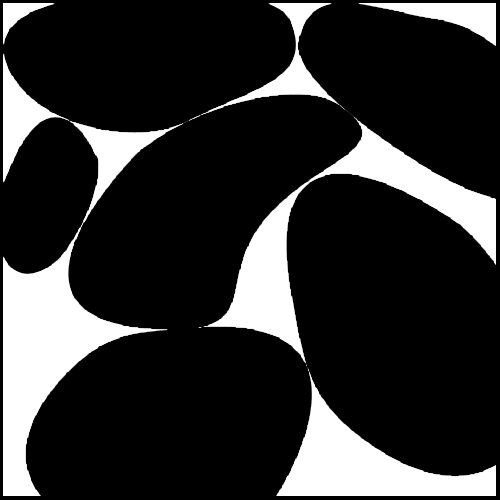
\includegraphics[width=0.7\textwidth]{figures/mineral_grains.png}
	\caption{Mineral grains} \label{fig:pore_void_space_mineral_grains}
\end{subfigure}
\begin{subfigure}[b]{0.49\textwidth}
	\centering
	
\includegraphics[width=0.7\textwidth]{figures/fractures.png}
	\caption{Fractures} \label{fig:pore_void_space_fractures}
\end{subfigure}
\caption{Illustration of volume between mineral grains and fracture voids in rocks. White color indicates void space where fluids can reside. Black color indicates mineral structures.}
\label{fig:pore_void_space}
\end{figure}

For so-called \emph{immiscible} (non-mixing) fluids the volume available for hydrocarbons, the \emph{hydrocarbon pore volume}, is limited by residual water in the pore space, called the \emph{irreducible water saturation} $S_{\text{wc}}$ of the rock \citep{dake_fundamentals_1978}. This water cannot be displaced by the hydrocarbon components, effectively reducing the available pore volume $\phi$ with a factor $S_{\text{wc}}$. Thus the hydrocarbon pore volume becomes $\vert V \vert \phi(1 - S_{wc})$. In the following it is assumed that the porosity is adjusted according to the irreducible water saturation, allowing us to use $\vert V \vert \phi$ for the hydrocarbon pore volume.

The porosity is obviously an essential parameter for a petroleum reservoir in that it limits the amount of space available for fluid components. What the porosity does not tell us about is the ease with which fluids flow through the formation. A rock with completely isolated pore spaces could in theory have a very high porosity, but without fluid flow between pore spaces oil and gas extraction would be impossible. Thus, the \emph{permeability} $\vec{K}$ of the rock is introduced \citep{jain_ch._2013}. $\vec{K}$ measures the degree of interconnectivity between the pore spaces. A high permeability indicates that it is easy for fluids to pass through the rock. As here, $\vec{K}$ is often given as a tensor since the media in which fluid flows can be anisotropic. That is, the permeability is directional dependent and varies between the different spatial directions. Table \ref{table:rock_permeabilities} shows a few typical absolute value permeability ranges, along with a classification and examples of rock types with the relevant properties. The table is modified from \citet{bear_dynamics_1972}.
\begin{table}
\caption{Typical permeability ranges for petroleum reservoir rock formations. Modified from source: Table 5.5.1 in \citep[p.~136]{bear_dynamics_1972}.} 
\label{table:rock_permeabilities}
\centering
\begin{tabular}{ M{2.5cm} | M{2.5cm} | M{4.5cm} N }
\bf{Permeability} 		      & \bf{Rocks} 			   & Range of $\log_{10}(K) [mD]$ &\\[1.1ex]\hline
Pervious 				      & Fracture rock 			   & $10^8$ to $10^4$   &\\[1.1ex]\hline
\multirow{2}{*}{Semipervious} & Oil Rock 	      			   & $10^4$ to $10$   &\\[1.1ex]\cline{2-3}
					      & \multirow{2}{*}{Sandstone}  & $10$ to $1$   &\\[1.1ex]\cline{1-1}\cline{3-3}
\multirow{3}{*}{Impervious}     & 					   & $1$ to $0.1$ &\\[1.1ex]\cline{2-3}
	 				      & Dolomite 				   & $0.1$ to $10^{-3}$ &\\[1.1ex]\cline{2-3}
 					      & Granite 				   & $10^{-3}$ to $10^{-5}$ &\\[1.1ex]\hline
\end{tabular}
\end{table}

The permeable regions where hydrocarbons flow are of little use if the valuable components escape to the surface. Laymen often think of oil and gas reservoirs as underground ``pools'' of fluids. The reality is not that far off, except that the geometry is inverses;  light petroleum components escape towards the surface and are trapped in an upside down pool by low-permeability geological formations, or in some cases by special hydrological phenomena \citep{jain_ch._2013}. Light components such as natural gas, if present, are found in the top layer, while the heavier oil is found just above the water aquifer in the bottom of the region.
%\begin{table}
%\centering
%\begin{tabular}{l | c | c | c | c | c | c}
%\bf{Permeability} & Pervious & \multicolumn{2}{ c | }{Semipervious} &  \multicolumn{3}{ c }{Impervious} \\
%\hline
%\bf{Rocks} & Fractured rock & Oil Rock &  \multicolumn{2}{ c | }{Sandstone} & Dolomite & Granite \\
%\hline
%$\log_{10}(K)$ [D] & [8,4] & [4,1] & [1,0] & [0,-1] & [-1,-3] & [-3,-5] \\
%\end{tabular}
%\caption{Typical permeability ranges for petroleum reservoir rock formations. Modified from source: Table 5.5.1 in \citep[p.~136]{bear_dynamics_1972}.} \label{table:rock_permeabilities}
%\end{table}
%%%%%%%%%%%%%%%% DRIVING MECHANISMS %%%%%%%%%%%%%%%%
\subsection{Driving Mechanisms of Production}
Petroleum components are harvested by drilling wells with perforations in the reservoir region, where pressure differences in the fluid drives it towards the surface. The natural pressure of the reservoir is often sufficient to drive the initial production. Continued production of hydrocarbon is driven by one or more of four mechanisms; solution gas drive, gas cap drive, natural water drive, and compaction drive \citep{dake_fundamentals_1978}. Removal of fluids from the reservoir causes a pressure drop. When the pressure is lowered compressible components expand and push the fluid components out of the rock formations. This is the cause of the three first drivers. In particular, gas drive is caused by expansion of oil and gas in solution. A lowering of pressure causes these components to precipitate and expand the volume of fluids, causing an evacuation of the rock formation. A gas cap or an aquifer, if present, will also expand under lowered pressure, again pushing down (or up in the case of water) on the oil strata and forcing it out of the reservoir region. The last driving mechanism, compaction drive, is caused by a collapse in the rock formation following the removal of supporting fluids. The collapse of the rock matrix forces remaining fluid out of the void space. All of these processes are part of the \emph{primary recovery} of the oil field. Primary recovery usually accounts for no more than $15\%$ of the oil in place \citep{tzimas_enhanced_2005}.

After the natural pressure drive of the reservoir weakens so called \emph{secondary recovery} is used. These techniques expend energy to increase the production potential of the reservoir. The most common secondary recovery technique is water injection, but other fluid types are also used. In the North Sea the primary and secondary oil recovery ranges between $45\%$ and $55 \%$ of original oil in place \citep{green_enhanced_2003}. 

The last category of the so called \emph{enhanced oil recovery} techniques, \emph{tertiary recovery}, seeks to alter the fluid and rock properties in the reservoir to improve the flow. These techniques are usually employed towards the end of the lifetime of a field, and are known to give an extra $5\%$ to $15\%$ of production \citep{tzimas_enhanced_2005}. It is worth noting that in modern petroleum reservoirs all three levels of recovery techniques are used in every part of the lifecycle of a field according to need, contrary to the hierarchical naming convention.

%%%%%%%%%%%%%%%% RESERVOIR MODELS %%%%%%%%%%%%%%%%
\section{Petroleum Reservoir Modeling}
\label{section:reservoir_modeling}
\begin{figure}
\centering
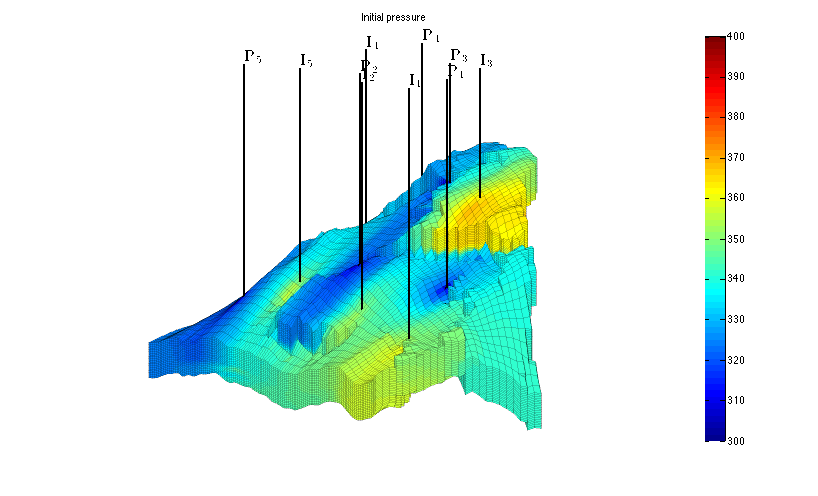
\includegraphics[trim=3cm 0cm 2cm 0cm,width=0.8\textwidth]{figures/saigup_field_pressure.png}
\caption{Example of a stratigraphic grid model of the Saigup field with wells and initial pressure data \citep{saigup_2003}.}
\label{fig:saigup_field_pressure}
\end{figure}
An oil reservoir is a complex and extensive structure. To run fluid simulations on the full scale model we need to identify and store the important properties of the rock formations together with information about the fluids contained within the hydrocarbon pore volume. These data points are gathered from the field by core samples, fluid samples, and seismic and electromagnetic geological exploration. The data gathered from field studies are compiled into a reservoir model containing all relevant parameters about the physical reservoir. Parameters like the permeability tensor $\vec{K}$, porosity $\phi$, phase saturation $S_l$ for phase $l$, and pressure $p$ are averaged and assigned to blocks representing subdomains of the model. This discrete version of the reservoir is closely connected to the discretized domain used when solving the fluid equations, as discussed in Section \ref{section:seq_splitting_method}. These static parameters represent the geological model, which (at least in our discussion) does not change throughout the lifetime of the field. The reservoir model also includes any injection or production wells and relevant well equations. An example of a grid on a rock formation is shown in Figure \ref{fig:saigup_field_pressure}. Here, the wells are shown as black lines and the pressure in each cell is indicated with color. This example uses a typical \emph{stratigraphic} grid, which allows for a semi-structured grid while retaining the layered nature of the rock formations. It is on such discrete versions of the domain we will develop the flow equations. The reservoir model also includes a \emph{fluid model}, a set of principles and equations chosen to model the hydrocarbon and water components present in the rock formations. Finally, the external interfaces of the reservoir are described. These include production and injection wells, and any fluxes across the outer boundaries of the reservoir, although \emph{no-flow boundaries} are usually assumed. We start by deriving a \emph{continuity equation} from the principle of \emph{mass conservation}.

%%%%%%%%%%%%%%%% THE CONTINUITY EQUATION %%%%%%%%%%%%%%%%
\subsection{The Continuity Equation}
\label{section:continuity_equation}
Conservation of mass is an important concept in fluid dynamics. It effectively states that mass can be neither created nor destroyed. This implies that the amount of mass in a closed system is constant. Here "closed" is taken to mean closed to mass and energy transfer, since thermodynamical processes also cause mass transfer according to the principle of \emph{mass-energy equivalence}.
%\citep{einstein_considerations_1940}
Even for thermodynamically open systems the conservation of mass is a relatively good approximation at reasonable energy levels. The continuity equation follows from conservation of mass by considering a \emph{control volume} $V \subset \mathbb{R}^d$, $d \in \{1,2,3\}$, over which we track mass exchange, see Figure \ref{fig:control_volume} for an example in two dimensions ($d = 2$). For a material with density $\rho$ we can compute the mass $m$ in the control volume at time $t$ by a volume integral of $\rho(\vec{x},t)$ over $V$, where $\vec{x} \in \mathbb{R}^d$ is a point in $V$:
\begin{equation*}
m = \int \limits_{V} \rho(\vec{x},t) \differential{V}.
\end{equation*}
If the concentration of some quantity in $V$ is measured by $\varphi$ we can do a similar integral and compute the amount in the control volume at time $t$ by
\begin{equation*}
\varphi_V(t) = \int \limits_{V} \varphi(\vec{x},t)\rho(\vec{x},t) \differential{V}.
\end{equation*}
This assumes that the conserved quantity is chemically inert, i.e., that there is no mass transfer between the conserved material and the other components in the control volume, and that no sources are present.
\tikzsetnextfilename{control_volume_V}
\begin{figure}[ht]
\centering
\begin{tikzpicture}
    \node[anchor=south west,inner sep=0] (image) at (0,0) {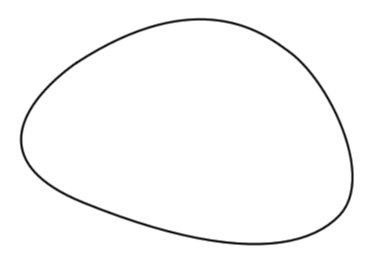
\includegraphics[width=0.5\textwidth]{figures/controlVolume.png}};
    \begin{scope}[x={(image.south east)},y={(image.north west)}]
        \node [left] at (0.5,0.5) {$V$};
        \node [right] at (0.85,0.79)  (normal) {$\vec{\nu}$};
        \draw [ultra thick, ->] (0.84,0.70) -- (0.95,0.80);
        \node [right] at (0.92,0.59) (flux) {$\vec{f}$};
        \draw [ultra thick, ->] (0.84,0.70) -- (1.07,0.65);
    \end{scope}
\end{tikzpicture}
\caption{A control volume $V \subset \mathbb{R}^2$ with boundary $\partial V$, unit surface normal $\vec{\nu}$ and a flux $\vec{f}$.}
\label{fig:control_volume}
\end{figure}
We now open the boundary $\partial V$ of $V$ and start tracking the mass transfer out of the control volume. The movement across $\partial V$ sets up a flux $\vec{f}$. Letting $\differential{\vec{v}}$ be an infinitesimal part of $\partial V$ with an outward facing unit normal $\vec{\nu}$ we can compute the mass transfer by
\begin{equation*}
 \int \limits_{\partial V} \vec{f} \cdot \vec{\nu} \differential{\vec{v}},
\end{equation*}
where $\vec{f} \cdot \vec{\nu}$ is the transport of the preserved quantity across $\differential{\vec{v}}$. Further, the change in the concentration of the preserved quantity within $V$ is measured by the temporal derivative of $\varphi_V(t)$:
\begin{equation*}
\frac{\partial \varphi_V(t)}{\partial t} = \text{change in $\varphi_V(t)$ during $\differential{t}$}.
\end{equation*}
Sources, either negative (sinks) or positive (sources), are introduced through a source term $q(\vec{x},t)$. Integrating over the control volume gives the total source term $q_{\text{tot}} = \int_V q(\vec{x},t) \differential{V}$. By convention, $q > 0$ is treated as an injection into the control volume. We now arrive at the complete conservation principle as applied to the control volume $V$:
\begin{equation} \label{eq:conservation_principle}
\frac{\partial \varphi_V(t)}{\partial t} = \int\limits_{V} q(x,t) \differential{V} - \int \limits_{\partial V} \vec{f} \cdot \vec{\nu} \differential{v}.
\end{equation}
We now use the \emph{divergence theorem}, see e.g. \citep[p.~68-69]{weber_essential_2003}, to relate the boundary flux to the divergence inside the control volume:
 \begin{equation} \label{eq:divergence_theorem}
 \int \limits_{\partial V} \vec{f} \cdot \vec{\nu} \differential{v} = \int \limits_{V} \nabla \cdot \vec{f} \differential{V}.
 \end{equation}
The boundary flux term now transforms directly to a control volume formulation, allowing us to gather the terms in the same integral, giving
\begin{equation*}
 \int \limits_{V} \left[ \frac{\partial{}}{\partial{t}} \left[ \varphi(x,t)\rho(x,t) \right] + \nabla \cdot \vec{f} - q(x,t) \right] \differential{V} = 0.
\end{equation*}
This works under the assumption of sufficient smoothness of the flux (for the divergence theorem) and the concentration and density (for the time derivative to move inside the integral), and by the linearity of the integral operation. Finally we arrive at the \emph{continuity equation} for the quantity of concentration $\varphi$:
\begin{equation} \label{eq:general_conservation_equation}
\frac{\partial{}}{\partial{t}} \left[ \varphi(x,t)\rho(x,t) \right] + \nabla \cdot \vec{f} = q(x,t).
\end{equation}
Here we have used the fact that the control volume $V$ is chosen arbitrarily, which implies that we can drop the integral sign without destroying the equality. If needed the source term can be modified to track mass transfer between components. The mass conservation relation results from Equation (\ref{eq:general_conservation_equation}) by setting $\varphi = 1$ and defining the mass flux $\vec{f} = \rho \vec{u}$, where $\vec{u}$ is the fluid velocity. Using a subscript for the time derivative we get the mass continuity equation:
\begin{equation} \label{eq:mass_conservation_equation}
\rho_t + \nabla \cdot \left( \rho \vec{u} \right) = q.
\end{equation}

So far we have assumed that the fluid phases can fill the control volume $V$ completely. As mentioned before, the porosity $\phi$ of the rock formations in the reservoir measures the available pore space. The porosity can be introduced into the continuity equation by letting it scale the total mass in the control volume, giving 
\begin{equation} \label{eq:mass_conservation_equation_porosity}
\left( \phi \rho \right)_t + \nabla \cdot \vec{f} = q.
\end{equation}
Here the temporal and spatial arguments are dropped for brevity. Equation (\ref{eq:mass_conservation_equation_porosity}) only models a single fluid \emph{phase}. A more advanced fluid description is introduced in the next section. 

%%%%%%%%%%%%%%%%  FLUID MODELS %%%%%%%%%%%%%%%%
\subsection{Fluid Models}
\label{section:fluid_models}
An important part of the reservoir model is the fluid description. The crude oil usually contains dissolved gas and the presence of a water phase is also common. A standard approach to fluid modeling is to use a compositional model where each hydrocarbon component, or at least a pseudo-component combining several chemical species, is subject to a mass balance equation. The fluid is described using three phases; the water, liquid and gas phase. In addition we introduce the mass fractions $C_{kg}$ and $C_{ko}$, that is, the mass fraction of component $k$ present in the gas and oil phase, respectively. Now the conditions $\sum_{k=1}^{n_c} C_{k \alpha} = 1, \alpha = \{g,o\},$ hold for a system with $n_c$ components. The mass-balance equations become
\begin{equation*}
( \phi (C_{kg} \rho_g S_g + C_{ko} \rho_o S_o) )_t + \nabla \cdot (C_{kg} \vec{f}_g + C_{ko} \vec{f}_o) = q_k,
\end{equation*}
for all components $k$, in addition to a standard continuity equation for water. The compositional fluid model will not be pursued further here.

At surface pressure and temperature the fluids from the reservoir separate into three phases; oil, gas, and water. The \emph{black-oil model} assumes that this holds in the reservoir too. Three pseudo-phases are assumed; a liquid phase, a gaseous phase, and a water phase. The black-oil model includes gas in solution through the \emph{solution gas-oil ratio}:
\begin{equation*}
R_{so} = \frac{\text{volume of gas evolved from oil at std. conditions}}{\text{volume of oil at std. conditions}}. 
\end{equation*}

$R_{so}$ is used to modify the density of the oil phase in order to account for the dissolved gas. Assuming three fluid phases implies three conservation laws, one for each phase. We model each of these phases by defining the \emph{phase saturation} $S_l$ of phase $l \in \{w,g,o\}$, denoting water, gas, and oil, respectively. The saturation of a phase measures the ratio of the amount of fluid of the given phase to the available hydrocarbon pore volume in the control volume $V$. The restriction 
\begin{equation} \label{eq:saturation_constraint}
\sum_l S_l = 1,
\end{equation} 
called the \emph{saturation constraint}, is rather obvious since we assume that the phases fill the entire available pore volume. In the two phase case the restriction becomes $S_w + S_o = 1$. Introducing the phase saturation into Equation (\ref{eq:mass_conservation_equation_porosity}) produces the phase continuity equation
\begin{equation} \label{eq:continuity_phase}
( \phi S_l \rho_l )_t + \nabla \cdot \vec{f}_l = q_l.
\end{equation}
Since the oil can contain gas in solution we need to modify the densities accordingly. Introducing the oil and gas density at standard condition, $\rho_{o}^{s}$ and $\rho_{g}^{s}$, respectively, the liquid oil density $\rho_{o}^{l}$ and the gaseous oil density $\rho_{o}^{g}$, we can express the reservoir density of oil as 
\begin{equation*}
\rho_o = \frac{\rho_o^s+\rho_g^s R_\text{so}}{B_o} = \rho_{o}^{l} + \rho_{o}^{g}, 
\end{equation*}
where $B_o$ is the \emph{formation volume factor}, the ratio of volume of oil at reservoir conditions to the volume of oil at standard (surface) conditions. That is,
\begin{equation*}
B_{o} = \frac{\text{volume of oil at reservoir conditions}}{\text{volume of oil at std. conditions}}. 
\end{equation*}
This gives the following set of black oil equations which we will use, where gas in solution is taken into account:
\begin{subequations}
\label{eq:black_oil_model}
\begin{align}
( \phi S_w \rho_w )_t + \nabla \cdot \vec{f}_w &= q_w, \\
( \phi S_o \rho_{o}^{l} )_t + \nabla \cdot \vec{f}_o &= q_o, \\
( \phi S_g \rho_g + \phi S_o \rho_{o}^{g} )_t + \nabla \cdot \vec{f}_l &= q_g.
\end{align}
\end{subequations}

%%%%%%%%%%%%%%%%%%%%%%%%%%%%%%%
%%%%%%%%%%%%%%%%  NUMERICAL METHODS %%%%%%%%%%%%%%%%%%%%%
\chapter{Numerical Methods} \thispagestyle{chapterpage}
\label{chapter:numerical_methods}
In practice we want to use the black oil model equations from Section \ref{section:fluid_models}  to predict fluid flow in the reservoirs. Closed form algebraic solutions are only available for the simplest problems, e.g. the Buckley-Leverett problem \citep{buckley_mechanism_1942}. For real life reservoirs we need to use \emph{numerical methods} to solve the system of equations. Different solution procedures have been proposed, and seen extensive use, throughout the years. Examples include, but are not limited to, the \emph{simultaneous solution method} \citep{aziz_petroleium_1979,molenaar_multigrid_1995}, the \emph{IMPES method} \citep{fagin_a-new_1966,coats_note_2000,aziz_petroleium_1979}, and the \emph{sequential implicit method}, also called the \emph{sequential splitting method} or the \emph{sequential solution method} \citep[chap. 5]{macdonald_methods_1970,spillette_a-high-stability_1973,aziz_petroleium_1979,aarnes_introduction_2007}. The latter method will be presented and used here.

The \emph{sequential splitting method} is presented in Section \ref{section:seq_splitting_method} before we introduce the \emph{finite volume method} in Section \ref{section:fvm} which we use to develop discrete fluid flow equations for the pressure in Section \ref{section:pressure_solver} and transport in Section \ref{section:transport_solver}. We conclude the chapter by presenting a number of numerical root finders used to solved the residual transport equations resulting from the discretization of the transport equation from Section \ref{section:transport_solver}.

%%%%%%%%%%%%%%%%  SEQUENTIAL SPLITTING %%%%%%%%%%%%%%%%
\section{Sequential Splitting}
\label{section:seq_splitting_method}
The black oil equations, Equation (\ref{eq:black_oil_model}), are coupled through the saturation constraint, Equation (\ref{eq:saturation_constraint}). In order to solve this coupled set of equations we want to rewrite the system to a form with a single unknown. To this end we introduce two tools; a per-phase version of \emph{Darcy's law}, 
\begin{equation} \label{eq:darcy}
\vec{u}_l = -\vec{K}\lambda_l(\nabla p_l - \rho_l\vec{g}),
\end{equation}
and the \emph{capillary pressure}
\begin{equation} \label{eq:capillary_pressure_definition}
p_{cow} = p_o - p_w.
\end{equation}
Darcy's law, first described by \citet{darcy_les_1856}, is a semi-empirical law relating pressure, gravity effects, and flow velocity of fluids in a porous medium. In this formulation we follow the velocity $\vec{u}_l$ and pressure $p_l$ of phase $l$. In Darcy's law, $\vec{K}$ is the absolute permeability tensor, and $\lambda_l$ the \emph{mobility}, defined by  
\begin{equation} \label{eq:mobility}
\lambda_l = \frac{ k_{rl} }{ \mu_{l} }.
\end{equation} 
$k_{rl}$ is the \emph{relative permeability} for phase $l$. $k_{rl}$ is modeled heuristically  according to the properties of the components in the reservoir. In the following $k_{rl} = S_l^2$ will be used. We also define the total mobility $\lambda = \sum_l \lambda_l$. The absolute and relative permeability defines the parameter $k_l = \vec{K}k_{rl}$, the permeability of phase $l$. This number quantifies the ease with which each phase moves through the rock formation. Here we will limit the discussion to a two phase immiscible incompressible black oil model. Thus we drop the gas equation and the $R_{\text{so}}$ part of the oil equation in Equation (\ref{eq:black_oil_model}).

Together with boundary conditions the multi phase continuity equation and Darcy's law model the dynamics of the fluids in a reservoir through a coupled system of partial differential equations. Additional effects like compressibility can be accounted for within this framework, see e.g. \citep{aziz_petroleium_1979}. The sequential splitting method works by decoupling the system of equations into a pressure equation and a saturation equation, also called the transport equation. The decoupling is done by using the saturation constraint from Equation (\ref{eq:saturation_constraint}) together with the Darcy law in Equation (\ref{eq:darcy}) and the capillary pressure defined in Equation (\ref{eq:capillary_pressure_definition}). These relations allow us to eliminate the oil variables $S_o$ and $p_o$ from the continuity equation and Darcy's law, giving two non-linear PDEs with the water saturation $S_w$ and water pressure $p_w$ as primary variables. Having obtained separate equations for the pressure and transport we can solve the two equations sequentially with separate implicit methods suited for each type of problem. We start out with an initial saturation in the reservoir, which is fed into the implicit pressure solver. This produces an updated velocity field $\vec{u}$. The transport solver uses this updated $\vec{u}$ to compute new saturations, after which the process is restarted. At each invocation of the transport solver (resp. pressure solver) the flux field (resp. saturation field) is assumed known. That is, the values are evaluated at the previous time step, making them explicit in nature. The primary unknowns in the equations are evaluated at the current time step, making them implicit. This makes the sequential splitting method semi-implicit. Algorithm \ref{algorithm:sequential_splitting} shows pseudo code for the sequential splitting method. One assumes that this splitting introduces only small errors for incompressible reservoir simulations \citep[chap. 5.6]{aziz_petroleium_1979}. In the next two sections we develop the pressure and transport equations in more detail.
\begin{algorithm}[ht]
 \SetAlgoLined
 \KwData{$s_0$, $t_{end}$, $\Delta t$, reservoir grid and parameters}
 \KwResult{s}
 \CommentSty{Initialize saturation field}\;
 $s = s_0$\;
\CommentSty{Solve for initial pressure}\; 
 $p$ = PRESSURE-SOLVER($s_0$)\;
 $t = 0$\;
 \While{time $t$ is less than $t_{end}$}{
 	\CommentSty{Solve transport equation with pressure assumed constant}\;
 	$s$ = TRANSPORT-SOLVER($s$,$p$,$\Delta t$)\;
	\CommentSty{Solve pressure equation with saturation assumed constant}\;
	$p$ = PRESSURE-SOLVER($s$)\;
	\CommentSty{Advance time step}\;
	$t = t + \Delta t$\;
 }
 \caption{Pseudo code implementing the sequential splitting scheme, see Section \ref{section:seq_splitting_method}}
 \label{algorithm:sequential_splitting}
\end{algorithm}

%%%%%%%%%%%%%%%%  THE PRESSURE EQUATION %%%%%%%%%%%%%%%%
\subsection{The Pressure Equation}
\label{section:pressure_equation}
The derivation of the pressure equation loosely follows the notation and procedure from \citet{aarnes_introduction_2007} and \citet{lie_mathematical_2013}, and starts by assuming that the porosity $\varphi$ and density $\rho$ are constant in time, that is, incompressibility of rock formations and fluids. Now, by Equation (\ref{eq:mass_conservation_equation_porosity}), we obtain
\begin{equation*}
\nabla \cdot (\rho_l\vec{u}_l) = q_l,
\end{equation*}
since the temporal derivative vanishes. The flux is defined to be a mass flux such that $\vec{f}_l = \rho_l \vec{u}_l$, with $\vec{u}_l$ being the velocity of the fluid. Note that the equation is taken to be per phase $l \in \{w,o\}$. Dividing by the density and substituting the velocity using the Darcy law in Equation (\ref{eq:darcy}) yields the pressure equation for a single phase:
\begin{equation*}
\nabla \cdot ( -\vec{K}\lambda_l(\nabla p_l - \rho_l\vec{g}) ) = \frac{q_l}{\rho_l}.
\end{equation*}
Now we define the global velocity $\vec{u} = \vec{u}_w + \vec{u}_o$, giving an equation relating the water and oil pressure:
\begin{equation} \label{eq:pressure_water_oil}
\nabla \cdot \vec{u} = - \nabla \cdot ( \vec{K}\left[ \lambda_w(\nabla p_w - \rho_w\vec{g}) + \lambda_o(\nabla p_o - \rho_o\vec{g}) \right] ) = q',
\end{equation}
with a modified source term
\begin{equation*}
q' = \frac{q_w\rho_o + q_o\rho_w}{\rho_w\rho_o}.
\end{equation*}
We still have both the oil and water pressure as unknowns. Following \citet{chavent_mathematical_1982} we define a saturation dependent complementary pressure $p_c$ by
\begin{equation} \label{eq:complementary_pressure}
p_c(s_w) = \int\limits_{s_\text{wc}}^{s_w} f_w(s) \frac{\partial p_\text{cow}}{\partial s_w}(s) \differential{s}.
\end{equation}
Here, $s_\text{wc}$ denotes the irreducible water saturation discussed in Section \ref{section:introduction_petroleum_reservoirs} and we have defined the \emph{fractional flow function} for phase $l$ by
\begin{equation} \label{eq:fractional_flow_function}
f_l = \frac{\lambda_l}{\lambda}.
\end{equation}
We note that in the two phase case the fractional flow function becomes 
\begin{equation} \label{eq:fractional_flow_function_expanded}
f_l = \frac{k_{rl}}{k_{rl} + M k_{rn}},
\end{equation}
where $n$ indicates the second phase and the \emph{viscosity ratio} $M$ is defined by
\begin{equation} \label{eq:viscosity_ratio}
M = \frac{\mu_l}{\mu_n} > 0.
\end{equation}
\begin{figure}[ht]
\tikzsetnextfilename{fractional_flow_wrt_viscosity_ratio}
\centering
\begin{tikzpicture}
\begin{axis}[
	width=0.5\textwidth,
	height=0.35\textwidth,
	xlabel={$S$},
	ylabel={$f_w(S)$},
	xmin = 0,
	xmax = 1,
	ymin = 0,
	ymax = 1,
	domain = 0:1,
	%samples = 100,
	grid = major,
	legend style={
		cells={anchor=west},
		legend pos=outer north east,
	}
	]
	\addplot {x^2/(x^2+0.01*(1-x)^2)};
	\addplot {x^2/(x^2+0.1*(1-x)^2)};
	\addplot {x^2/(x^2+1*(1-x)^2)};
	\addplot {x^2/(x^2+10*(1-x)^2)};
	\addplot {x^2/(x^2+100*(1-x)^2)};
	\legend{M=0.01,M=0.1,M=1,M=10,M=100}
\end{axis}
\end{tikzpicture}
\caption{The fractional water flow function $f_w$, Equation (\ref{eq:fractional_flow_function}), with quadratic $k_{rl}$ and viscosity ratio $M$, Equation (\ref{eq:viscosity_ratio}).}%
\label{fig:fractional_flow_wrt_viscosity_ratio}%
\end{figure}%%
Figure \ref{fig:fractional_flow_wrt_viscosity_ratio} shows $f_w$ under the influence of different viscosity ratios. Note that $M < 1$ increases the $f_w$-value on the left hand side, while $M > 1$ lowers the $f_w$-values in the same region. Even moderate deviations from $M=1$ causes significant changes in $f_w$. The complementary pressure equation in Equation (\ref{eq:complementary_pressure}) takes care of the saturation dependency of the capillary pressure, giving a looser coupling between the pressure and transport equation \citep{aarnes_introduction_2007}. Taking the gradient of $p_c$ yields
\begin{align} \label{eq:complementary_pressure_gradient}
\nabla p_c = \nabla \int\limits_{s_\text{wc}}^{s_w} f_w(s) \frac{\partial p_\text{cow}}{\partial s_w}(s) \differential{s} &= \left[ f_w\frac{\partial p_\text{cow}}{\partial s_w} \right](s_w) - \left[ f_w\frac{\partial p_\text{cow}}{\partial s_w} \right](s_\text{wc}) \nonumber \\
	&= \left[ f_w\frac{\partial p_\text{cow}}{\partial s_w} \right](s_w) = f_w\nabla p_\text{cow},
\end{align}
by the fundamental theorem of calculus and the fact that $f_w(s_\text{wc}) = 0$. The purpose of $p_c$ is to define a \emph{global pressure} $p$ by
\begin{equation} \label{eq:global_pressure_definition}
p = p_o - p_c
\end{equation}
in order to rewrite the pressure equation to be dependent on the global pressure and saturation only. Gathering the gradient pressure terms in Equation (\ref{eq:pressure_water_oil}), and since $p_\text{cow} = p_o - p_w$, we get
\begin{equation*}
\lambda_w \nabla p_w + \lambda_o \nabla p_o = \lambda_w (\nabla p_o - \nabla p_\text{cow}) + \lambda_o \nabla p_o = \lambda \nabla p_o - \lambda_w p_\text{cow}.
\end{equation*}
Using the relation from Equation (\ref{eq:complementary_pressure_gradient}) and the global pressure definition in Equation (\ref{eq:global_pressure_definition}) we are able to express the gradients in terms of the global pressure only:
\begin{equation*}
\lambda_w \nabla p_w + \lambda_o \nabla p_o = \lambda \nabla p_o - \lambda_w p_\text{cow} = \lambda \nabla p_o - \lambda_w \frac{\nabla p_c}{f_w} = \lambda (\nabla p_o - \nabla p_c) = \nabla p.
\end{equation*}
Inserting this relation into Equation (\ref{eq:pressure_water_oil}) gives the global pressure equation, an \emph{elliptic} equation for the global pressure $p$:
\begin{equation} \label{eq:pressure_equation}
- \nabla \cdot ( \vec{K}\left[ \lambda\nabla p - (\lambda_w \rho_w + \lambda_o\rho_o)\vec{g} \right] ) = q'.
\end{equation}
%%%%%%%%%%%%%%%%  THE TRANSPORT EQUATION %%%%%%%%%%%%%%%%
\subsection{The Transport Equation}
\label{section:transport_equation}
Having found a pressure equation we need to complete the model by introducing the transport equation. We start out with the phase continuity equations in the black oil model as stated in Equation (\ref{eq:black_oil_model}), but drop the gas terms. These equations already contain the time derivative of the saturation, but we have a flow velocity term which we need to remove in order to have a single unknown. We do this by using Darcy's law from Equation (\ref{eq:darcy}) and the capillary pressure defined in Equation (\ref{eq:capillary_pressure_definition}), as in \citet{aarnes_introduction_2007}, to obtain
\begin{equation*}
\vec{K} \nabla p_{cow} = \vec{K}( \nabla p_o - \nabla p_w) =  (\vec{K}\rho_o\vec{g} - \frac{\vec{u}_o}{\lambda_o}) - (\vec{K}\rho_w\vec{g} - \frac{\vec{u}_w}{\lambda_w})
\end{equation*}
Inserting the total velocity $\vec{u} = \vec{u}_w + \vec{u}_o$ for $\vec{u}_o$ and multiplying by the mobilities, we get
\begin{equation*}
\lambda_o \lambda_w \vec{K} \nabla p_{cow} =  (\vec{K}\lambda_o \lambda_w\rho_o\vec{g} - \lambda_w \vec{u} + \lambda_w \vec{u}_w) - (\vec{K}\lambda_o \lambda_w \rho_w\vec{g} - \lambda_o\vec{u}_w).
\end{equation*}
Gathering terms and dividing by the total mobility $\lambda$ yields the following expression for the water velocity vector $\vec{u}_w$:
\begin{equation*}
\vec{u}_w = f_w \vec{u} + \vec{K} \lambda_o f_w \nabla p_{cow} + \vec{K} \lambda_o f_w \vec{g} (\rho_w - \rho_o).
\end{equation*}
Here we have used the fractional flow function $f_w$, see Equation (\ref{eq:fractional_flow_function}). Inserting this relation into the continuity equation, Equation (\ref{eq:continuity_phase}), and assuming constant porosity and density gives the following equation for the water saturation, and in extension the oil saturation (by the saturation constraint in Equation  (\ref{eq:saturation_constraint})):
\begin{equation} \label{eq:two_phase_transport}
\phi \frac{\partial S_w}{\partial t} + \nabla \cdot \left(f_w [ \vec{u} + \vec{K} \lambda_o \nabla p_{cow} + \vec{K}\lambda_o \vec{g} (\rho_w - \rho_o) ] \right) = \frac{q_w}{\rho_w}.
\end{equation}
This equation has both hyperbolic and parabolic properties \citep{aziz_petroleium_1979}. The coupled pressure and transport equations are solved using the procedure outlined in Algorithm \ref{algorithm:sequential_splitting}.

%%%%%%%%%%%%%%%% MATHEMATICAL MODEL %%%%%%%%%%%%%%%%
\subsection{Mathematical Model}
The black oil model, and in extension the pressure and transport equations, describes the spatial and temporal variation of the properties of the fluids in the reservoir. We solve these equations on the spatial domain $\Omega \subset \mathbb{R}^d$, where $d \in \{2,3\}$, from time $t=0$ to the final time $t=T$, giving the domain $\Omega^+ \coloneqq \Omega \times [0,T]$ for the partial differential equations, as sketched in Figure \ref{fig:spatial_temporal_domain}. The boundaries of this domain is denoted by $\partial \Omega^+ \coloneqq \partial \Omega \times [0,T]$. 
\tikzsetnextfilename{spatial_temporal_domain}
\begin{figure}
\centering
\begin{tikzpicture}[scale=0.5]
% TEXT
\node at (-0.5,3) (domain_time) {$\Omega \times [0,T]$};
\node at (6.5,4) (domain_top) {$\Omega$};
\node at (10.5,1) (domain_boundary) {$\partial \Omega$};
\draw [thick, ->] (domain_boundary) -- (9.5,1.9);
\begin{scope} % Top domain
\draw[ultra thick]
(2,6) 
to [out=0,in=300] (10,11)
to [out=120,in=10] (5,14)
to [out=190,in=80] (4,10)
to [out=260,in=180] (2,6);
\end{scope}
\begin{scope} % Bottom domain - solid
\clip (4.5,0) rectangle (10.4,4);
\draw[ultra thick]
(2,0) 
to [out=0,in=300] (10,5)
to [out=120,in=10] (5,8)
to [out=190,in=80] (4,4)
to [out=260,in=180] (2,0);
\end{scope}
\begin{scope} % Bottom domain - solid
\clip (0,0.3) rectangle (6,-0.3);
\draw[ultra thick]
(2,0) 
to [out=0,in=300] (10,5)
to [out=120,in=10] (5,8)
to [out=190,in=80] (4,4)
to [out=260,in=180] (2,0);
\end{scope}
\begin{scope} % Bottom domain - dashed
\draw[ultra thick, dashed]
(2,0) 
to [out=0,in=300] (10,5)
to [out=120,in=10] (5,8)
to [out=190,in=80] (4,4)
to [out=260,in=180] (2,0);
\end{scope}
\draw[ultra thick] % Left straight line
(1.5,0.3)
to [out=90,in=270] (1.5,6.3);
\draw[ultra thick] % Right straight line
(10.33,4)
to [out=90,in=270] (10.33,10);
\draw[ultra thick, dashed] % Top straight line
(5,8)
to [out=90,in=270] (5,14);
\end{tikzpicture}
\caption{The spatial and temporal domain $\Omega^+ = \Omega \times [0,T]$ for the partial differential equations in the black oil model, Equation (\ref{eq:black_oil_model}). The spatial domain has border $\partial \Omega$.} \label{fig:spatial_temporal_domain}
\end{figure}
In order to have a well posed problem, we need \emph{initial} and \emph{boundary conditions}. That is, we have to know the initial value at time $t = 0$ of all variables and how the equations behave at the boundaries $\partial \Omega^+$ of the domain $\Omega^+$. The initial condition $S_w(\vec{x},0) = S_w^0(\vec{x})$, $S_0\colon \Omega \to [0,1]$, allows us to compute the corresponding initial pressure field $p(\vec{x},0)$ by the pressure equation in Equation (\ref{eq:pressure_equation}), giving a complete initial condition. Common boundary conditions for reservoir simulations includes flow rate (Neumann type) and pressure (Dirichlet type) conditions. The Dirichlet and Neumann part of the boundary is denoted by $\partial \Omega_D$ and $\partial \Omega_N$, respectively. Note that $\partial \Omega_D \cap \partial \Omega_N = \emptyset$. The pressure boundary condition becomes
\begin{equation*} %\label{eq:transport_dirichlet_condition}
p(\vec{x}) = p_D(\vec{x}),~\forall \vec{x} \in \partial \Omega_D
\end{equation*}
where $\partial \Omega_D \subset \partial \Omega$ and $p_D\colon\partial \Omega_D \to \mathbb{R}_+$ is some scalar pressure function . Rate conditions can be specified as
\begin{equation*} %\label{eq:transport_neumann_condition}
\vec{v}\cdot \vec{\nu} = [-\vec{K}\lambda(\nabla p - \rho \vec{g})](\vec{x}) \cdot \vec{\nu}= Q_{\partial \Omega_N}(\vec{x}),~\forall ~\vec{x} \in \partial \Omega_N,
\end{equation*}
using the unit surface normal $\vec{\nu}$ of $\partial \Omega$ and Darcy's law, see Equation (\ref{eq:darcy}). The magnitude of the rate at the Neumann part of the boundary, $\partial \Omega_N \subset \partial \Omega$, is defined by the function $Q_{\partial \Omega_N}\colon\partial \Omega_N\to \mathbb{R}$. The default rate boundary condition is a \emph{no-flow} condition, i.e. $\vec{v}\cdot \vec{\nu} = Q_{\partial \Omega_N} = 0$, indicating that no fluid particles will cross the domain boundary.

The transport and pressure equation over the domain $\Omega^+$, along with boundary conditions, combines to the following problem:
%\begin{subequations}
%\label{eq:transport_pressure_boundary_system}
\begin{align*}
\phi S_w(\vec{x},t)_t + \nabla \cdot \left(f_w \alpha(\vec{x},t) \right) &= q_w(\vec{x},t)\rho_w^{-1},~~(\vec{x},t) \in \Omega^+, \\
- \nabla \cdot ( \vec{K}(\vec{x})\left[ \lambda\nabla p(\vec{x},t) - (\lambda_w \rho_w + \lambda_o\rho_o)\vec{g} \right] ) &= q(\vec{x},t),~~(\vec{x},t) \in \Omega^+, \\
S_w(\vec{x},0) &= S_0(\vec{x}),~~\vec{x} \in \Omega, \\
[-\vec{K}\lambda(\nabla p - \rho \vec{g})](\vec{x},t) \cdot \vec{\nu} &= Q(\vec{x},t),~~(\vec{x},t) \in \partial \Omega^+,
\end{align*}
%\end{subequations}
where $\alpha(\vec{x},t) = [ \vec{u}(\vec{x},t) + \vec{K}(\vec{x}) ( \lambda_o \nabla p_{cow} + \lambda_o \vec{g} (\rho_w - \rho_o)) ]$ and we have used Neumann boundary conditions. In order to solve these equations we will use the \emph{finite volume method}, or FVM, as presented in the following section.

%%%%%%%%%%%%%%%% FVM %%%%%%%%%%%%%%%%
\section{The Finite Volume Method}
\label{section:fvm}
The finite volume method is a discretization technique for solving differential equations. It is well suited for elliptic, parabolic, and hyperbolic equations, and is a natural choice for conservation laws because of the control volume formulation of the method and the the fact that it lends itself to implementation on a wide range of grid types, including unstructured grids. The idea behind the method is to express a balance over each control volume, making the FVM \emph{conservative} in the sense that the numerical flux is conserved between neighboring control volumes. In other words, the conservation of quantities over any group of control volumes is exact \citep{patankar_numerical_1980}.
Another strength is the natural and intuitive formulation of the method.

The finite volume method is defined over discrete control volumes of the domain. We proceed by using the domain $\Omega$ from Figure \ref{fig:spatial_temporal_domain}. We let $\mathcal{T}$ be a mesh on $\Omega$ such that $\bigcup_{V \in \mathcal{T}} V = \Omega$, where $V$ is a control volume. The finite volume method expresses an integral flux balance for each such control volume $V$. In general the control volumes can be of any shape, but a usual choice is to let every $V$ be a polygonal convex subset of $\Omega$ such that $V \cap K = \emptyset, ~\forall (V,K) \in \mathcal{T}\times\mathcal{T}, V \neq K$ \citep{eymard_finite_2000}. The collection of sides $s$ of the polygon $V$ is denoted $E_V$. Note that the term "polygonal" is is used for both polygonal two-dimensional control volumes with $d=2$ and polyhedral three-dimensional control volumes with $d=3$. Figure \ref{fig:spatial_domain_mesh} shows an example of a polygonal mesh on the two dimensional domain $\Omega$. Notice that the mesh coverage of the domain is only partial due to the straight edges of the grid cells. The error introduced by this discrepancy is assumed to be negligible in the theoretical setup. In practice the domain, i.e. the reservoir, consists of grid cells taken from the geological model of the rock formations. Such a grid is typically of a polyhedral type, removing the partial coverage problem altogether. The precise formulation of the FVM is introduced by applying it to the pressure and transport equations.
\tikzsetnextfilename{spatial_domain_grid}
\begin{figure} [ht]
\centering
\begin{tikzpicture}[scale=0.6,every node/.style={draw,circle,fill=black,inner sep=0.05cm}]
\node [draw=none,fill=none] at (8.8,10.2) (control_colume) {$V_i$};
\node [draw=none,fill=none] at (3,10) (domain) {$\Omega$};

%%% MESH %%%
\node at (6.5,12) (i1) {};
\node at (7,10) (i2) {};
\node at (5,8) (i3) {};
\node at (3,6.9) (i4) {};

\node at (6,14.08) (o1) {};
\node at (4.07,13) (o2) {};
\node at (4.2,11) (o3) {};
\node at (4,9.5) (o4) {};
\node at (2.8,7.7) (o5) {};
\node at (2,7,) (o6) {};
\node at (2,6) (o7) {};
\node at (4,6.2) (o8) {};
\node at (8,7.3) (o9) {};
\node at (10.1,9) (o10) {};
\node at (9.6,11.6) (o11) {};
\node at (8,13.36) (o12) {};

\draw [thick] (i1) -- (i2);
\draw [thick] (i2) -- (i3);
\draw [thick] (i3) -- (i4);

\draw [thick] (i1) -- (o1);
\draw [thick] (i1) -- (o2);
\draw [thick] (i1) -- (o3);
\draw [thick] (i1) -- (o11);
\draw [thick] (i1) -- (o12);

\draw [thick] (i2) -- (o3);
\draw [thick] (i2) -- (o3);
\draw [thick] (i2) -- (o4);
\draw [thick] (i2) -- (o9);
\draw [thick] (i2) -- (o10);
\draw [thick] (i2) -- (o11);

\draw [thick] (i3) -- (o4);
\draw [thick] (i3) -- (o5);
\draw [thick] (i3) -- (o8);
\draw [thick] (i3) -- (o9);

\draw [thick] (i4) -- (o5);
\draw [thick] (i4) -- (o6);
\draw [thick] (i4) -- (o7);
\draw [thick] (i4) -- (o8);

\draw [thick] (o1) -- (o2);
\draw [thick] (o2) -- (o3);
\draw [thick] (o3) -- (o4);
\draw [thick] (o4) -- (o5);
\draw [thick] (o5) -- (o6);
\draw [thick] (o6) -- (o7);
\draw [thick] (o7) -- (o8);
\draw [thick] (o8) -- (o9);
\draw [thick] (o9) -- (o10);
\draw [thick] (o10) -- (o11);
\draw [thick] (o11) -- (o12);
\draw [thick] (o12) -- (o1);

%%% DOMAIN %%%
\begin{scope} % Top domain
\draw[ultra thick]
(2,6) 
to [out=0,in=300] (10,11)
to [out=120,in=10] (5,14)
to [out=190,in=80] (4,10)
to [out=260,in=180] (2,6);
\end{scope}
\end{tikzpicture}
\caption{The domain $\Omega$, see Figure \ref{fig:spatial_temporal_domain}, with a grid $\mathcal{T}$ consisting of triangular control volumes $V_i$.}
\label{fig:spatial_domain_mesh} 
\end{figure}

%%%%%%%%%%%%%%%%  PRESSURE SOLVER. %%%%%%%%%%%%%%%%
\section{Pressure Solver}
\label{section:pressure_solver}
The pressure equation in (\ref{eq:pressure_equation}) is solved by the FVM method. We start by integrating over a grid cell $V$:
\begin{equation*}
\int\limits_V - \nabla \cdot ( \vec{K}\left[ \lambda\nabla p - (\lambda_w \rho_w + \lambda_o\rho_o)\vec{g} \right] ) \differential{V} = \int\limits_V q' \differential{V}.
\end{equation*}
The left hand side integral is split into two parts, allowing us to isolate the pressure. Using the divergence theorem, and assuming that $\vec{K}\lambda\nabla p$ is smooth, we obtain
\begin{equation} \label{eq:pressure_integral_conservation_form}
-\int\limits_{\partial V} ( \vec{K}\lambda\nabla p ) \cdot \vec{\nu} \differential{v}  = \int\limits_{\partial V} (\vec{K}(\lambda_w \rho_w + \lambda_o\rho_o)\vec{g}) \cdot \vec{\nu} \differential{v} + q' \differential{V}.
\end{equation}
Exploiting the polygonal geometry of the grid cells we can write
\begin{equation*}
-\int\limits_{\partial V} ( \vec{K}\lambda\nabla p ) \cdot \vec{\nu} \differential{v} = -\sum\limits_{s \in E_V} \int\limits_{s} ( \vec{K}\lambda\nabla p ) \cdot \vec{\nu}_s \differential{v}.
\end{equation*}
Thus, our task reduces to approximating the integral $\int_{s} ( \lambda\vec{K}\nabla p ) \cdot \vec{\nu}_s \differential{v}$ on each edge $s$ of the cell. To this end we introduce a one-sided transmissibility $t_V^s$ defined by
\begin{equation*}
t_V^s = \frac{\vec{\nu}_s \vec{K}_V \Delta \vec{c}_V^s}{\lVert \Delta \vec{c}_V^s \rVert^2},
\end{equation*}
where $\vec{\nu}_s$ is the surface normal of $s$ with magnitude equal to $m(s)$, $\vec{K}_V$ is the permeability tensor for the current cell, and $\Delta\vec{c}_V^s = \vec{c}_s - \vec{c}_V$ is the face-to-cell centroid difference vector. Here $\vec{c}_V$ is the \emph{centroid} of cell $V$ while $\vec{c}_s$ is the centroid of face $s$. Further, the function $m\colon\mathcal{T}\to\mathbb{R}_+$ is the $d$-dimensional \emph{Lebesgue-measure}, which computes the ``size'' of the control volume, see e.g. \citep{eymard_finite_2000}. When $d=2$ this function gives the \emph{area} of the control volume $V$, while $d=3$ gives the \emph{volume}. We will also use the function $m\colon E\to \mathbb{R}_+$, the $d-1$-dimensional Lebesgue measure to be used on edges $s$ of $V$. No confusion should arise from this double definition of $m$ since the correct version should be apparent from the context. Now we can express the integral on the edge $s$ connecting $V$ and $K$ using the \emph{two-point flux approximation} scheme, the TPFA scheme, expressed as
\begin{equation*}
\int\limits_s (\vec{K}\nabla p_s) \cdot \vec{\nu} \differential{v} = (p_V - p_K)\left(\frac{1}{t_V^s} + \frac{1}{t_K^s}\right)^{-1} = \frac{t_V^s t_K^s}{t_V^s + t_K^s} (p_V - p_K).
\end{equation*}
A mobility weighted version becomes 
\begin{equation*}
\int\limits_s (\lambda\vec{K}\nabla p_s) \cdot \vec{\nu}\differential{v} = (p_V - p_K)\left(\frac{1}{\lambda_V t_V^s} + \frac{1}{\lambda_K t_K^s}\right)^{-1},
\end{equation*}
where $\lambda_V$ is the total mobility in $V$. This result is inserted into Equation (\ref{eq:pressure_integral_conservation_form}), such that we obtain
\begin{equation*}
-\sum\limits_{s \in E_V} (p_V - p_K)\left(\frac{1}{\lambda_V t_V^s} + \frac{1}{\lambda_K t_K^s}\right)^{-1} = \int\limits_{\partial V} (\vec{K}(\lambda_w \rho_w + \lambda_o\rho_o)\vec{g}) \cdot \vec{\nu} \differential{v} + \int\limits_V q' \differential{V}.
\end{equation*}
The right hand side of Equation (\ref{eq:pressure_integral_conservation_form}) is approximated in a similar manner. The integral of the gravity term over the boundary is approximated by the following relation:
\begin{equation*}
\int\limits_{\partial V} (\vec{K}(\lambda_w \rho_w + \lambda_o\rho_o)\vec{g}) \cdot \vec{\nu} \differential{v} = \sum\limits_{s \in E_V}  \vec{g} [\Delta \vec{c}_V^s \omega_V + \Delta \vec{c}_K^s \omega_K] \left(\frac{1}{\lambda_V t_V^s} + \frac{1}{\lambda_K t_K^s}\right)^{-1},
\end{equation*}
where $\omega_V = \frac{\lambda_{wV}\rho_w + \lambda_{oV}\rho_o}{\lambda_V}$. The source term $q'$ is simply integrated over the control volume and expressed as a discrete value $q_V'$ for each $V$. 
This results in the following linear system to be solved for the pressure in each control volume $V$:
\begin{equation*}
-\sum\limits_{s \in E_V} (p_V - p_K) T_s = \vec{g} [\Delta \vec{c}_V^s \omega_V + \Delta \vec{c}_K^s \omega_K] T_s + q_V',~\forall V \in \mathcal{T},
\end{equation*}
Here we have defined the \emph{mobility weighted transmissibility} $T_s$ by
\begin{equation*}
T_s = \left(\frac{1}{\lambda_V t_V^s} + \frac{1}{\lambda_K t_K^s}\right)^{-1},
\end{equation*}
where $K$ is the unique neighbor cell to $V$ such that $\partial V \cap \partial K = s$.

The next section introduces the finite volume method applied to the transport solver. Since the method essentially expresses a balance equation over the control volume at hand we will need to know the fluid fluxes across the boundary $\partial V$. One of the assumptions of the sequential splitting method is that these face fluxes can be computed based on the pressure field from the current iteration. The face fluxes $F_s$ for face $s$ are computed by
\begin{equation} \label{eq:pressure_face_fluxes}
F_s = T_s(p_V-p_K+F_s^g),~\forall s \in E, (V,K) \in \mathcal{T}\times\mathcal{T} : \partial V \cap \partial K = s,
\end{equation}
where the gravity flux $F_s^g$ is defined as
\begin{equation*}
F_s^g = (\Delta \vec{c}_V^s + \Delta \vec{c}_K^s)\vec{g}.
\end{equation*}

%%%%%%%%%%%%%%%%  TRANSPORT SOLVER %%%%%%%%%%%%%%%%
\section{Transport Solver}
\label{section:transport_solver}
The \opm code assumes that the transport problem can be solved in two steps by splitting Equation (\ref{eq:two_phase_transport}) into a buoyant and a viscous-capillary equation. That is, first
\begin{equation} \label{eq:two_phase_transport_visc_pc}
\phi \partial_t S_w + \nabla \cdot \left(f_w [ \vec{u} + \lambda_o \vec{K} \nabla p_{cow} ] \right) = q_w(\vec{x},t)\rho_w^{-1},~~(\vec{x},t) \in \Omega^+
\end{equation}
is solved for the saturation influenced by viscous and capillary forces, and sources before 
\begin{equation} \label{eq:two_phase_transport_gravity}
\phi \partial_t S_w + \nabla \cdot \left( f_w \lambda_o \vec{K} \vec{g} (\rho_w - \rho_o)  \right) = 0,~~(\vec{x},t) \in \Omega^+
\end{equation}
is solved for the gravity influenced saturation. The variables $\vec{x}$ and $t$ are dropped for brevity. We start by integrating the viscous-capillary transport equation from Equation (\ref{eq:two_phase_transport_visc_pc}) over each control volume $V \in \mathcal{T}$:
\begin{equation*}
\int\limits_V \phi \partial_t S_w(\vec{x},t)+ \nabla \cdot \left(f_w [ \vec{u} + \lambda_o \vec{K} \nabla p_{cow} ] \right) - \frac{q_w(\vec{x},t)}{\rho_w} \differential{V} = 0,~\forall V \in \mathcal{T}.
\end{equation*}
This gives
\begin{equation} \label{eq:transport_eq_fvm_raw}
\phi_V \frac{\partial }{\partial t} \int\limits_V S_w \differential{V} + \int\limits_{\partial V} \left(f_w [ \vec{u} + \lambda_o \vec{K} \nabla p_{cow} ] \right) \cdot \vec{\nu} \differential{v} - \int\limits_{V} \frac{q_w}{\rho_w } \differential{V} = 0,~\forall V \in \mathcal{T}
\end{equation}
by the divergence theorem and under the assumptions that $S_w$ is sufficiently smooth and that the porosity $\phi$ is a given constant $\phi_{V}$ for each grid cell. We now express the cell averaged water saturation $S_V$ for cell $V$ as
\begin{equation} \label{eq:cell_saturation_definition}
S_V = \frac{1}{m(V)} \int\limits_V S_w \differential{V}.
\end{equation}
$S_V$ will be used as a representation of the saturation in the cell and is one of the primary variables in the final system of equations. Now the source term is integrated over $V$, giving a discrete source
\begin{equation} \label{eq:cell_production_definition}
q_V = \int\limits_{V} q_w \differential{V}.
\end{equation}
This leaves only the treatment of the boundary integral term. Letting $s \in E_V$ be the edges of $V$ and $\vec{\nu}_s$ be the outward facing unit normal of the edge $s$, we can express the boundary integral as
\begin{equation*}
\int\limits_{\partial V} \left(f_w [ \vec{u} + \lambda_o \vec{K} \nabla p_{cow} ] \right) \cdot \vec{\nu} \differential{v} = \sum\limits_{s \in E_V} \left[ \int\limits_s \left(f_w [ \vec{u} + \lambda_o \vec{K} \nabla p_{cow} ] \right) \cdot \vec{\nu}_s \differential{v} \right],
\end{equation*}
since $\partial V = \bigcup_{s \in E_V} \bar{s}$.  $\bar{s}$ is the \emph{closure} of side $s$. The pressure solver handles each edge integral, see Section \ref{section:pressure_solver}, but a few comments are in order here regardless. The \emph{upwind method} will be used to compute the interface fluxes. That is, on each edge $s$ shared by two control volumes, say $V$ and $K$, a scalar approximation $F_s$ of the flux is chosen such that the information is gathered in the cell the flow is coming from. This flux was calculated by the pressure solver, and is shown in Equation (\ref{eq:pressure_face_fluxes}). The fluxes over $\partial V$ can be categorized as either incoming or outgoing fluxes. The set of edges with incoming fluxes for cell $V$ is denoted $E_V^+$, while the set of edges with outgoing fluxes is denoted $E_V^-$. The fractional flow value for the incoming fluxes are independent of the local cell saturation $S_V$ and distinct for each edge, and will be denoted by $f_s$. This allows us to denote the incoming flow as 
\begin{equation*}
Q_V^+ = \sum\limits_{s \in E_V^+} f_s F_s
\end{equation*}
and the outgoing flow as
\begin{equation*}
Q_V^- = \sum\limits_{s \in E_V^-} f_w(S_V) F_s = f_w(S_V) \sum\limits_{s \in E_V^-} F_s = f_w(S_V) F_V^-,
\end{equation*}
where $F_V^-$ is the total outgoing flux. Note that because of the upwind method only the flow out of cell $V$ is influenced by the local saturation $S_V$. Summing the flow terms over all edges of $V$ yields
\begin{equation*}
\sum\limits_{s \in E_V} \left[ \int\limits_s \left(f_w [ \vec{u} + \lambda_o \vec{K} \nabla p_{cow} ] \right) \cdot \vec{\nu}_s \differential{v} \right] = f_w(S_V)F_V^- + Q_V^+.
\end{equation*}
Inserting this into Equation (\ref{eq:transport_eq_fvm_raw}), using (\ref{eq:cell_saturation_definition}) and (\ref{eq:cell_production_definition}) and dividing by the cell "volume" $m(V)$ and the porosity $\phi_{V}$ we obtain
\begin{equation} \label{eq:transport_equation_semi_discrete}
\frac{\partial S_V}{\partial t} + \frac{1}{m(V)\phi_V} \left[ f_w(S_V)F_V^- + Q_V^+ \right] - \frac{q_V}{\rho_w \phi_V} = 0,~\forall V \in \mathcal{T}
\end{equation}
By averaging values over the control volume and using the upwind method we have arrived at a semi-discretized version of the transport equation. Now we must choose a technique for resolving the time derivative in the first term of the Equation (\ref{eq:transport_equation_semi_discrete}). We approximate the derivative by
\[ \frac{\partial S_V}{\partial t} = \frac{S_V^{n+1} - S_V^n}{\Delta t} + \mathcal{O}(\Delta t), \]
where the superscript $n$ denotes the current \emph{time level} corresponding to the chosen \emph{time step} $\Delta t$. That is, the current time is $t = n\Delta t,$ where $n \in [0,1,2,\dots,n_{\text{max}}]$ and $n_{\text{max}} = \ceil{\frac{T}{\Delta t}}$. Now we can choose between an \emph{explicit} and an \emph{implicit} scheme by setting the time level of the other terms in the equation. Explicit difference schemes put severe restrictions on the time step $\Delta t$, e.g. through a CFL condition, as first described in \citet{courant_uber_1928}, and becomes unstable for time steps exceeding this limit. Implicit schemes are much more robust and are known to give unconditional stability, see e.g. \citep{aziz_petroleium_1979}. We want to exploit the extra stability of the implicit scheme, and thus choose to evaluate the other $S_V$-dependent terms at the new time level, that is, $f_w = f_w(S_V^{n+1})$.

One remark is in order here. In writing out Equation (\ref{eq:transport_equation_semi_discrete}) we have made a few shortcuts by skipping the dependent variables of the various terms. The cell saturation is obviously time dependent, but the interface fluxes $F_s$ also have a saturation dependency. In a pure implicit approach these saturation values should also be taken at the new time level $n+1$, but the assumption of known interface fluxes implies $F_s = F_s(S_V^n)$, that is, the fluxes are evaluated at the current time level. This is an explicit approach. This mixing of implicit and explicit terms gives rise to the semi-implicit nature of the sequential splitting method (a similar approach is used in the IMPES method). Inserting the time derivative approximation and using the implicit scheme we arrive at the residual form of the discrete viscous-capillary transport equation, plotted for a single cell $V$ as a function of $\Delta t$ and $S_V^{n+1}$ in Figure \ref{fig:residual_two_phase_transport}:
\begin{align} \label{eq:residual_two_phase_transport}
R(S_i^{n+1};S_i^n, \Delta t) &\coloneqq S_V^{n+1} - S_V^n - \frac{\Delta t}{m(V)\phi_V} \left[ f_w(S_V^{n+1})F_V^- + Q_V^+ \right] - \frac{q_V \Delta t}{\rho_w \phi_V} \nonumber \\
&= 0,~\forall V \in \mathcal{T}.
\end{align}
\tikzsetnextfilename{residual}
\begin{figure}
\centering
\begin{tikzpicture}%
    \begin{axis}[
            view={-60}{30},
            width=0.6\textwidth,
            height=0.3\textheight,
            xlabel={$\Delta t$},
            ylabel={$S^{n+1}$},
            zlabel={$R(S^{n+1},\Delta t)$},
            xmajorgrids,
	    ymajorgrids,
	    zmajorgrids
            ]
        \addplot3[surf,shader=faceted] table[col sep=comma,trim cells=true,x=dt, y=snp, z=Rnp] {datafiles/one_cell_residual-s-1_000000.data};
    \end{axis}
\end{tikzpicture}%
\caption{The residual from Equation (\ref{eq:residual_two_phase_transport}) as a function of $\Delta t$ and $S^{n+1}$. }
\label{fig:residual_two_phase_transport}
\end{figure}

A similar approach is used on Equation (\ref{eq:two_phase_transport_gravity}), the gravity transport equation. The \opm code assumes that the grid for this problem is aligned in vertical columns, which holds for the stratigraphical grids often used in reservoir simulation packages, as discussed in Section \ref{section:introduction_petroleum_reservoirs}. Further it assumes that the gravity effects are only influencing the saturation in cells above or below a cell, allowing solution of the transport equations on a per column basis. The gravity terms on the interface to neighboring cells are approximated using the transmissibility and a centroid difference, as was the case for the viscous-capillary equation. These boundary fluxes are gathered in an edge flux variable, say $F_s^g$ for each edge $s \in E_V$, and are constant throughout a simulation since they only depend on permeabilities, constant densities, and the grid configuration. Note that the flux on edges in the $x$-$z$ and $y$-$z$ planes are zero, since the cells are assumed to be vertically aligned and the gravitational influence only works in the vertical direction. The FVM requires the mobilities $\lambda_l$ to be evaluated on each interface edge $s$, a task again accomplished by the upwind method. Since gravity causes the lightest phase to move upwards the mobility for this phase must be taken from the cell below the current edge. Likewise the mobility for the heavy phase is gathered from the cell above the current edge. Figure \ref{fig:mobility_upwind} illustrates this for a heavy water phase and a light oil phase. 
\tikzsetnextfilename{mobility_upwind}%
\begin{figure}[ht]%
\centering
\begin{tikzpicture}[scale=0.8]%
     \draw [step=2.0,very thick] (0,0) grid (2,6);
     \node at (1,3) (V) {V};
     \node at (1,1) (L) {L} edge[->,bend right] (V.south east) edge[<-,bend left] (V.south west);
     \node at (1,5) (K) {K} edge[->,bend right] (V.north west) edge[<-,bend left] (V.north east);
     
      \draw [thick, ->] (2.3,4.3) -- (2.3,3.7);
      \node [right] at (2.3,4) {$F_{s_t}^g \geq 0$};
      
      \draw [thick, ->] (2.3,2.3) -- (2.3,1.7);
      \node [right] at (2.3,2) {$F_{s_b}^g < 0$};
      
      \node at (0.26,2.33) {$w$};
      \node at (0.26,4.33) {$w$};
      \node at (1.72,1.69) {$o$};
      \node at (1.72,3.69) {$o$};
      
       \draw [thick, ->] (-0.4,3.3) -- (-0.4,2.7);
       \node [left] at (-0.4,3) {$\vec{g}$};
\end{tikzpicture}%%
\caption{The flow of a light oil phase $o$ and a heavy water phase $w$ in a grid with vertically aligned cells  $K,V,L$ and interface edges $s_t,s_b$. The gravitational force is directed downwards in the figure.}%
\label{fig:mobility_upwind}%
\end{figure}%
Denoting the top face of cell $V$ as $s_t$ and the bottom face as $s_b$, we arrive at the following residual equation to be solved:
\begin{align} \label{eq:residual_two_phase_transport_gravity}
R_g(S_i^{n+1}) &\coloneqq S_V^{n+1} - S_V^n  \nonumber \\
&- \frac{\Delta t}{m(V)\phi_V} \left[ \frac{\lambda_w(S_K^{n})\lambda_o(S_V^{n+1})}{\lambda_w(S_K^{n})+\lambda_o(S_V^{n+1})} F_{s_t}^g + \frac{\lambda_w(S_V^{n+1})\lambda_o(S_L^{n})}{\lambda_w(S_V^{n+1})+\lambda_o(S_L^{n})} F_{s_b}^g \right] \nonumber \\
&= 0,~(K,L) \in \mathcal{T}\times \mathcal{T} : K\cap V = s_t, L\cap V = s_b, ~\forall V \in \mathcal{T}.
\end{align}
Here the phase mobilities $\lambda_l$ are evaluated explicitly in the neighboring cells using the cell saturation $S_K^{n}$ and $S_L^{n}$ according to the configuration in Figure \ref{fig:mobility_upwind}. That is, $\lambda_w(S_K^n)$ and $\lambda_o(S_L^n)$ are known a priori when solving Equation \ref{eq:residual_two_phase_transport_gravity}. The single cell gravity residual is shown in Figure \ref{fig:residual_two_phase_transport_gravity}
\tikzsetnextfilename{residual_gravity}
\begin{figure}[ht]
\centering
\begin{tikzpicture}%
    \begin{axis}[
            view={-60}{30},
            width=0.6\textwidth,
            height=0.3\textheight,
            xlabel={$\Delta t$},
            ylabel={$S^{n+1}$},
            zlabel={$R_g(S^{n+1},\Delta t)$},
            xmajorgrids,
	    ymajorgrids,
	    zmajorgrids
            ]
        \addplot3[surf,shader=faceted] table[col sep=comma,trim cells=true,x=dt, y=snp, z=Rnp] {datafiles/one_cell_residual_grav.data};
    \end{axis}
\end{tikzpicture}%
\caption{The gravity residual from Equation (\ref{eq:residual_two_phase_transport_gravity}) as a function of $\Delta t$ and $S^{n+1}$. Here $s_0 = 0.5$, $\mu_w = \mu_o = \unit[1]{mD}$, $F_{s_t}^g = \unitfrac[10^{-5}]{m^3}{s}$, $F_{s_t}^g = \unitfrac[-10^{-5}]{m^3}{s}$, $m(V)\phi_V = \unit[500]{m^3}$, $\lambda_w(S_K^n) = \unit[500]{m^{-2}}$, and $\lambda_o(S_L^n) = \unit[150]{m^{-2}}$.}
\label{fig:residual_two_phase_transport_gravity}
\end{figure}

We now want to solve Equations (\ref{eq:residual_two_phase_transport}) and (\ref{eq:residual_two_phase_transport_gravity}) by finding roots of the residuals $R(S_V^{n+1})$ and $R_g(S_V^{n+1})$. Existence of solutions of these residual equations is hard to prove with rigor. Despite this a solution is assumed to exist for well-posed reservoir simulation residuals for every time step $\Delta t$ \citep{younis_adaptively_2010}. Further, if brackets $[a,b]_R$ and $[c,d]_{R_g}$ can be found according to Definition \ref{definition:bracket} we know that a solution exists by Theorem \ref{theorem:ivt} and the continuity of the residuals.

%%%%%%%%%%%%%%%%  REORDERING %%%%%%%%%%%%%%%%
\subsection{Reordering}
\label{section:reordering}
The upwind method is used for the discretization of the flow equations. This choice of discretization ensures that the state of a cell $i$ is only affected by the state in the upwind neighboring cells $U(i)$, creating a well defined domain of dependence for each cell. The upwind direction is based on the fluid flux on the border between neighboring cells. An example of a discretization with interface flux directions is shown in Figure \ref{fig:discretization_velocity_natural_numbering_sparsity_pattern} along with the sparsity pattern resulting from a standard numbering of the cells in the grid. The system of equations calls for a full matrix solve since the resultant matrix is in a non-triangular form even after using the upwind method, i.e. after removing all downwind cells from the matrix. This can be amended by \emph{reordering} the cells in the domain according to the flow direction.

The approach can be motivated by viewing the domain as a directed graph with the cells as nodes and the interface fluxes determining the edge directions between nodes. In computer science, a topological sort is an algorithm designed to order the nodes in a directed graph according to the direction of the interconnecting edges. The sorting algorithm provides a list of nodes such that all edges from every node points to nodes with a higher ordering in the list. In fluid flow terms this approach provides an ordering of the cells according to the domain of influence for each cell. A cell early in the ordering is independent of the subsequent cells in the list, allowing the state of each cell in the ordering to be computed sequentially.  
In other words, the new numbering gives a lower triangular matrix which indicates that the system of equations for the cell saturations can be solved sequentially by a forward substitution. Figure \ref{fig:discretization_velocity_topological_numbering_sparsity_pattern} shows the cell numbering and sparsity pattern resulting from a topological sort of the cells from the example domain in Figure \ref{fig:discretization_velocity_natural_numbering_sparsity_pattern}. Note the lower triangular structure of the matrix after removing all downwind cells.
\begin{figure}[ht]
\centering
\tikzsetnextfilename{3x3_grid_natural_numbering}
\begin{subfigure}[b]{0.43\textwidth}
\begin{tikzpicture}
    \node[anchor=south west,inner sep=0] (image) at (0,0) {
\includegraphics[width=\textwidth]{figures/3_by_3_grid.png}};
    \begin{scope}[x={(image.south east)},y={(image.north west)}]
        \draw [ultra thick, ->] (0.28,0.16) -- (0.38,0.16);
        \draw [ultra thick, ->] (0.62,0.16) -- (0.72,0.16);
        
        \draw [ultra thick, ->] (0.16,0.3) -- (0.16,0.4);
        \draw [ultra thick, ->] (0.5,0.3) -- (0.5,0.4);
        \draw [ultra thick, ->] (0.83,0.3) -- (0.83,0.4);
        
        \draw [ultra thick, ->] (0.38,0.49) -- (0.28,0.49);
        \draw [ultra thick, ->] (0.62,0.49) -- (0.72,0.49);
        
        \draw [ultra thick, ->] (0.16,0.63) -- (0.16,0.73);
        \draw [ultra thick, ->] (0.5,0.63) -- (0.5,0.73);
        \draw [ultra thick, ->] (0.83,0.63) -- (0.83,0.73);
        
        \draw [ultra thick, ->] (0.38,0.82) -- (0.28,0.82);
        \draw [ultra thick, ->] (0.72,0.82) -- (0.62,0.82);
        
        \node at (0.16,0.16)  (normal) {1};
        \node at (0.5,0.16)  (normal) {2};
        \node  at (0.83,0.16)  (normal) {3};
        
        \node at (0.16,0.49)  (normal) {4};
        \node  at (0.5,0.49)  (normal) {5};
        \node  at (0.83,0.49)  (normal) {6};
        
        \node  at (0.16,0.82)  (normal) {7};
        \node  at (0.5,0.82)  (normal) {8};
        \node  at (0.83,0.82)  (normal) {9};
    \end{scope}
\end{tikzpicture}
\caption{Cell numbering and fluid flow direction.}
\label{fig:discretization_velocity_natural_numbering}
\end{subfigure}%
~
\tikzsetnextfilename{3x3_array_natural_numbering}
\begin{subfigure}[b]{0.5\textwidth}
\centering
\begin{tikzpicture}
	\begin{axis}[%
	width=\textwidth,%
	height=\textwidth,%
	y dir=reverse,%
	xtick=data,%
	ytick=data]%
	\addplot[mark options={blue},only marks]%
	table[col sep=comma, trim cells=true,x=x, y=y] {datafiles/sparsity_pattern_normal_upwind.data};%
	\addplot[mark options={red},only marks]%
	table[col sep=comma, trim cells=true,x=x, y=y] {datafiles/sparsity_pattern_normal_downwind.data};%
	\end{axis}
\end{tikzpicture}
\caption{Sparsity pattern. Downwind cells are shown using red markers.}
\label{fig:sparsity_pattern_natural_numbering}
\end{subfigure}%
\caption{Domain with natural numbering}
\label{fig:discretization_velocity_natural_numbering_sparsity_pattern}
\end{figure}

The topological ordering can always be generated provided that the graph is cycle free. That is, after leaving a node along an edge that node will never be revisited. This node structure results from a circulation free flux field $\vec{v}$ \citep{natvig_fast_2006,lie_fast_2013}. For incompressible flow, see \citet{natvig_fast_2006}, and cases with negligible or no gravity and capillary forces, see \citet{kwok_potential-based_2007,lie_fast_2013}, zero circulation is typical, at least with careful choice of numerical methods \citep{natvig_fast_2006,lie_fast_2013}. When introducing significant gravity and capillary effects, see \citet{kwok_potential-based_2007}, or compressible flow, see \citet{lie_fast_2013}, circulation can occur in the velocity field. On the discrete domain circulation appear as cycles or \emph{strongly connected components} in the graph. A strongly connected component is a group of nodes such that every node is reachable from every other node. These types of problems are not unusual in practice and as such is a big problem for the reordering approach since these groups represents irreducible blocks in the system of equations. One possible solution is to redefine the strongly connected component as a single pseudo node in the topological ordering, and solving this region as a separate problem using e.g. a modified Newton method or Gauss-Seidel iterations. Cycles can be found in linear time $\mathcal{O}(n)$ by either Tarjan's algorithm or by using a double depth first search, where $n$ is the number of cells in the discretization \citep{natvig_fast_2008}. Algorithm \ref{algorithm:reordering} outlines the reordering procedure used to solve the transport equation, see Equation (\ref{eq:two_phase_transport}).
\begin{figure}[ht]
\centering
\tikzsetnextfilename{3x3_grid_topological_numbering}
\begin{subfigure}[b]{0.43\textwidth}
\begin{tikzpicture}
    \node[anchor=south west,inner sep=0] (image) at (0,0) {
\includegraphics[width=\textwidth]{figures/3_by_3_grid.png}};
    \begin{scope}[x={(image.south east)},y={(image.north west)}]
        \draw [ultra thick, ->] (0.28,0.16) -- (0.38,0.16);
        \draw [ultra thick, ->] (0.62,0.16) -- (0.72,0.16);
        
        \draw [ultra thick, ->] (0.16,0.3) -- (0.16,0.4);
        \draw [ultra thick, ->] (0.5,0.3) -- (0.5,0.4);
        \draw [ultra thick, ->] (0.83,0.3) -- (0.83,0.4);
        
        \draw [ultra thick, ->] (0.38,0.49) -- (0.28,0.49);
        \draw [ultra thick, ->] (0.62,0.49) -- (0.72,0.49);
        
        \draw [ultra thick, ->] (0.16,0.63) -- (0.16,0.73);
        \draw [ultra thick, ->] (0.5,0.63) -- (0.5,0.73);
        \draw [ultra thick, ->] (0.83,0.63) -- (0.83,0.73);
        
        \draw [ultra thick, ->] (0.38,0.82) -- (0.28,0.82);
        \draw [ultra thick, ->] (0.72,0.82) -- (0.62,0.82);
        
         \node at (0.16,0.16)  (normal) {1};
        \node at (0.5,0.16)  (normal) {2};
        \node  at (0.83,0.16)  (normal) {5};
        
        \node at (0.16,0.49)  (normal) {4};
        \node  at (0.5,0.49)  (normal) {3};
        \node  at (0.83,0.49)  (normal) {6};
        
        \node  at (0.16,0.82)  (normal) {9};
        \node  at (0.5,0.82)  (normal) {8};
        \node  at (0.83,0.82)  (normal) {7};
    \end{scope}
\end{tikzpicture}
\caption{Cell numbering and fluid flow direction.}
\label{fig:discretization_velocity_topological_numbering}
\end{subfigure}%
~
\tikzsetnextfilename{3x3_array_topological_numbering}
\begin{subfigure}[b]{0.5\textwidth}
\centering
\begin{tikzpicture}
	\begin{axis}[%
	width=\textwidth,%
	height=\textwidth,%
	y dir=reverse,%
	xtick=data,%
	ytick=data]%
	\addplot[mark options={blue},only marks]%
	table[col sep=comma, trim cells=true,x=x, y=y] {datafiles/sparsity_pattern_topological_upwind.data};%
	\addplot[mark options={red},only marks]%
	table[col sep=comma, trim cells=true,x=x, y=y] {datafiles/sparsity_pattern_topological_downwind.data};%
	\end{axis}
\end{tikzpicture}
\caption{Sparsity pattern. Downwind cells are shown using red markers.}
\label{fig:sparsity_pattern_topological_numbering}
\end{subfigure}%
\caption{Domain with topological numbering}
\label{fig:discretization_velocity_topological_numbering_sparsity_pattern}
\end{figure}

\begin{algorithm}[ht]
 \SetAlgoLined
 \SetKw{In}{in}
 \KwData{Saturations $S_V$ in all cells $V$, fluxes $F_s$ on all faces $s$.}
 \KwResult{Updated saturations $S_V$}
 generate a topological ordering $\mathcal{T}_{\text{order}}$ of (pseudo) cells $V_{\text{order}}$ based on the face fluxes $F_s$\;
 \ForEach{(pseudo) cell $V_{\text{order}}$ \In $\mathcal{T}_{\text{order}}$}{
     \uIf{$V_{\text{order}}$ contains multiple cells $V$ from $\mathcal{T}$}{
     	solve the non-linear system for $S_V$ using a vector procedure, e.g. Gauss-Seidel iterations\;
     }
     \Else {
     	solve the single cell problem for $S_V$ using a scalar root finder, e.g. Regula Falsi\;
     }
 }
 \Return updated cell saturations $S_V$
 \caption{Pseudo code showing the reordering procedure for solving a transport problem, as in Equation (\ref{eq:two_phase_transport})}
\label{algorithm:reordering}
\end{algorithm}

%\begin{comment} % Comment for reordering cycle notes
%Directedness:
%\begin{quote}
%To see this, we rewrite (7) as $S_i^{k+1} = S_i^k + Q_i(S_i^{k+1})-F_i^{+}(S_i^{k+1})+F_i^{-}(S_j^{k+1};j\in U(i))$, where $F_i^+$ and $F_i^-$ are terms representing �ow out of and into cell $G_i$ and $U(i) = \{j | v_{ij} < 0\}$ denotes the indexes of the neighboring cells on the upstream side of $G_i$. In a cell $G_i$ penetrated by an injection well, $U(i) = empty$ and the saturation can thus be computed by solving (7) locally using a Newton method.
%Having found $S_i^{k+1}$, we can immediately update the saturation in all cells having $G_i$ as their only �in�ow
%neighbor� (i.e., in all $G_j$ for which $U(j) ? \{i\}$) and so on. This process can be continued if we are able
%to �nd a sequence of cells $p = (p_1, . . . , p_n)$ such that if $G_{pi}$ is on the upstream side of $G_{pj}$, then $p_i < p_j$.
%\citep{aarnes_fast_2006}
%\end{quote}
%
%\begin{quote}
%In the absence of gravity and capillary forces, all phases will be flowing in the same direction, ...
%\citep{kwok_potential-based_2007}
%\end{quote}
%
%No saturation or pressure dependencies, a simple topological potential ordering can be used.
%
%\begin{quote}
%In the presence of gravity, buoyancy forces can cause different phases to flow in opposite directions. The upstream direction for each phase $p$ is determined by the sign of $\Phi_{p,i}-\Phi_{p,l}$, where $\Phi_{p,i} = p_i-\gamma_pz_i$.
%\citep{kwok_potential-based_2007}
%\end{quote}
%
%This can introduce pressure dependencies on downstream equations/variables. Two different orderings are needed for three phase case. Can order on only water potential in two phase case.
%
%\begin{quote}
%So far, in the absence of capillary effects, the saturation dependence in each equation is purely upstream; thus, for a given phase, saturations downstream from cell $i$ do not appear in equation $i$. In contrast, equation $i$ involves phase pressure from all neighboring cells, be they upstream or downstream from cell $i$. Since we can only choose one phase pressure as a primary variable, the other phase pressures must be expressed as $p_q = p_p +P_{cpq}(S),$ where $p_p$ is the primary pressure and $p_q$ is the pressure of another phase.
%\citep{kwok_potential-based_2007}
%\end{quote}
%
%This can introduce saturation dependencies on downstream equations/variables. Must choose $p_w$ as primary pressure variable. No valid ordering for the gas equations when present.
%
%\begin{quote}
%The fact that viscous flow is unidirectional along streamlines will be the key property ...
%\citep{natvig_fast_2008}
%\end{quote}
%
%\begin{quote}
%In the absence of gravity, most flow models are unidirectional in the sense that $f > 0$ for scalar equations or that the Jacobian of $f$ has distinct, positive eigenvalues.
%\citep{natvig_fast_2008}
%\end{quote}
%
%\begin{quote}
%By using a discontinuous Galerkin scheme combined with an upwind flux approximation on cell interfaces, the directedness of (1) is preserved in the discrete system in the sense that the solution in an element only depends on the solutions in its immediate neighbors on the upwind side.
%\citep{natvig_fast_2008}
%\end{quote}
%
%\begin{quote}
%For incompressible flow, the exact velocity field has zero circulation. A simple argument shows that the same is true for an approximate velocity field computed by a two-point pressure solver. A mixed finite-element solution, on the other hand, may give a velocity field with nonzero circulation. In compressible flow, we may also get nonzero circulation. In our experience, cycles that appear in velocity fields computed by the mixed finite-element method are small and sparse for incompressible and weakly compressible flows.
%\citep{natvig_fast_2006}
%\end{quote}
%
%\begin{quote}
%Cycles correspond to groups of elements that are made mutually dependent by a nonzero circulation in the velocity field $\vec{v}.$
%\citep{natvig_fast_2006}
%\end{quote}
%
%\begin{quote}
%The dynamics of the transport problem is generally determined by the balance between viscous and gravity forces. For heavy-oil systems, however, gravity segregation is typically a weak effect compared to viscous flow because of large injection rates and small differences in the densities of the oil and water phases. This means that the transport will mainly be co-current, giving a unidirectional flow property that can be exploited to develop efficient transport solvers.
%\citep{lie_fast_2013}
%\end{quote}
%
%\begin{quote}
%If gravity is neglected and a monotone method like the standard two-point flux-approximation scheme is used to discretize the pressure equation, the velocity field $\vec{v}$ has no loops.
%\citep{lie_fast_2013}
%\end{quote}
%\end{comment} % Comment for reordering cycle notes

%%%%%%%%%%%% ROOT FINDERS %%%%%%%%%%%%%%%%%%%%
\subsection{Root Finders}
\label{section:root_finders}
The reordering approach breaks the large system of equations into smaller subproblems. The single cell problems involves solving a univariate equation for the saturation in each cell $V$, namely Equation (\ref{eq:residual_two_phase_transport}). That is, we want to find the \emph{root} of the residual $R$. In more general terms, given a function $f\colon\mathbb{R}\to\mathbb{R}$ we want to find the numbers $x$ such that $f(x) = 0$. The literature contains a long list of numerical root finding algorithms for such problems, a few of which will be tested here for the single cell solver. 

%%%%%%%%%%%%%%% BISECTION %%%%%%%%%%%%%%%%%
\subsubsection{The Bisection Method}
\label{section:bisection_method}
The bisection method is a simple and robust \emph{bracketing method}. That is, the method works over a \emph{bracket} of the function $f$ on the real line, using the following definition
\begin{definition} \label{definition:bracket}
A bracket $[a,b]_f$ for $f: \mathbb{R} \rightarrow \mathbb{R}$ is a closed subset of $\mathbb{R}$, say $[a,b] = \{x \in \mathbb{R} : a \leq x \leq b, a < b, f(a)f(b) < 0 \}$.
\end{definition}
Now we state the \emph{intermediate value theorem}, which will help guarantee the existence of a root in a given bracket:
\begin{theorem} \label{theorem:ivt} \textbf{Intermediate Value Theorem:}
Let $f\colon[a,b] \rightarrow \mathbb{R}$ be a continuous function on the closed interval $[a,b] = \{x \in \mathbb{R} : a \leq x \leq b \}$. Then for every value $y$, $f(a) < y < f(b)$, there exists a number $c \in (a,b)$ such that $f(c) = y$.
\end{theorem}
The proof of this theorem can be found in e.g \citep{binmore_mathematical_1977}. Using a bracket $[a,b]_f$ in Theorem \ref{theorem:ivt} quickly leads to the following corollary:
\begin{corollary} \label{corollary:root_existence}
Let $f\colon\mathbb{R} \rightarrow \mathbb{R}$ be a continuous function with a \emph{bracket} $[a,b]$. Then by Theorem \ref{theorem:ivt} there exists at least one number $r \in (a,b)$ such that $f(r) = 0$.
\end{corollary}
The corollary follows since the end points of the bracket are such that $f(a) < 0, f(b) > 0$ or, conversely, $f(a) > 0, f(b) < 0$, thereby bracketing the value $y = 0$ from the statement of Theorem \ref{theorem:ivt}.

Now, starting with a bracket $[a,c]_f$ the next iterate $b$ is found by halving the interval (hence the name of the method):
\begin{equation*}
b = \frac{a+c}{2}.
\end{equation*}
A new starting bracket is chosen from the points $a,b,c$ according to Definition \ref{definition:bracket}. The new bracket is named $[a,c]_f$ and the process is restarted. This iteration continues until a precise root is found, or the bracket becomes smaller than some tolerance $\epsilon$. By Corollary \ref{corollary:root_existence}, and the fact that the size of the bracket always decreases, the bisection method is guaranteed to converge. This is true in general for bracketing methods, although the convergence speed will vary. A more formal convergence theorem with proof can be found in \citet{kincaid_ch._2002}.

%%%%%%%%%%%%%%% REGULA FALSI %%%%%%%%%%%%%%%%%
\subsubsection{Regula Falsi}
\label{section:regula_falsi}
Another bracketing method is the \emph{regula falsi}, also called the \emph{false position method}. Again we start with a bracket $[a,c]_f$. The method computes a secant line between the two end points of the bracket, as illustrated in Figure \ref{fig:regula_falsi_secant}, using the following equation:
\begin{equation*}
y(x) = \frac{f(c) - f(a)}{c-a}(x-a) + f(a).
\end{equation*}
In the following we will use the notation $f_x \coloneqq f(x)$ to simplify the equations. Since the secant line $y(x)$ is a continuous function the bracket $[a,b]_f$ can be used as a bracket for $y$ as well, giving $[a,b]_y$. This implies, by Corollary \ref{corollary:root_existence}, that $\exists b \in (a,b) : y(b) = 0$. $b$ is found by
\begin{equation} \label{eq:regula_falsi_update}
b = a - f_a\frac{c-a}{f_c - f_a},
\end{equation}
the \emph{regula falsi step}. Now $b$ is used to update the bracket $[a,c]_f$ according to Definition \ref{definition:bracket}. This iteration is continued until a root is found or the bracket size falls below some tolerance $\epsilon$. Note that efficient implementations of the regula falsi requires only one function evaluation every iteration, since only one new point in the bracket is computed. Algorithm \ref{algorithm:regula_falsi} shows pseudo code for the \opm implementation of Regula Falsi.
\tikzsetnextfilename{regula_falsi_secant}
\begin{figure}[ht]
\centering
\begin{tikzpicture}
    \node[anchor=south west,inner sep=0] (image) at (0,0) {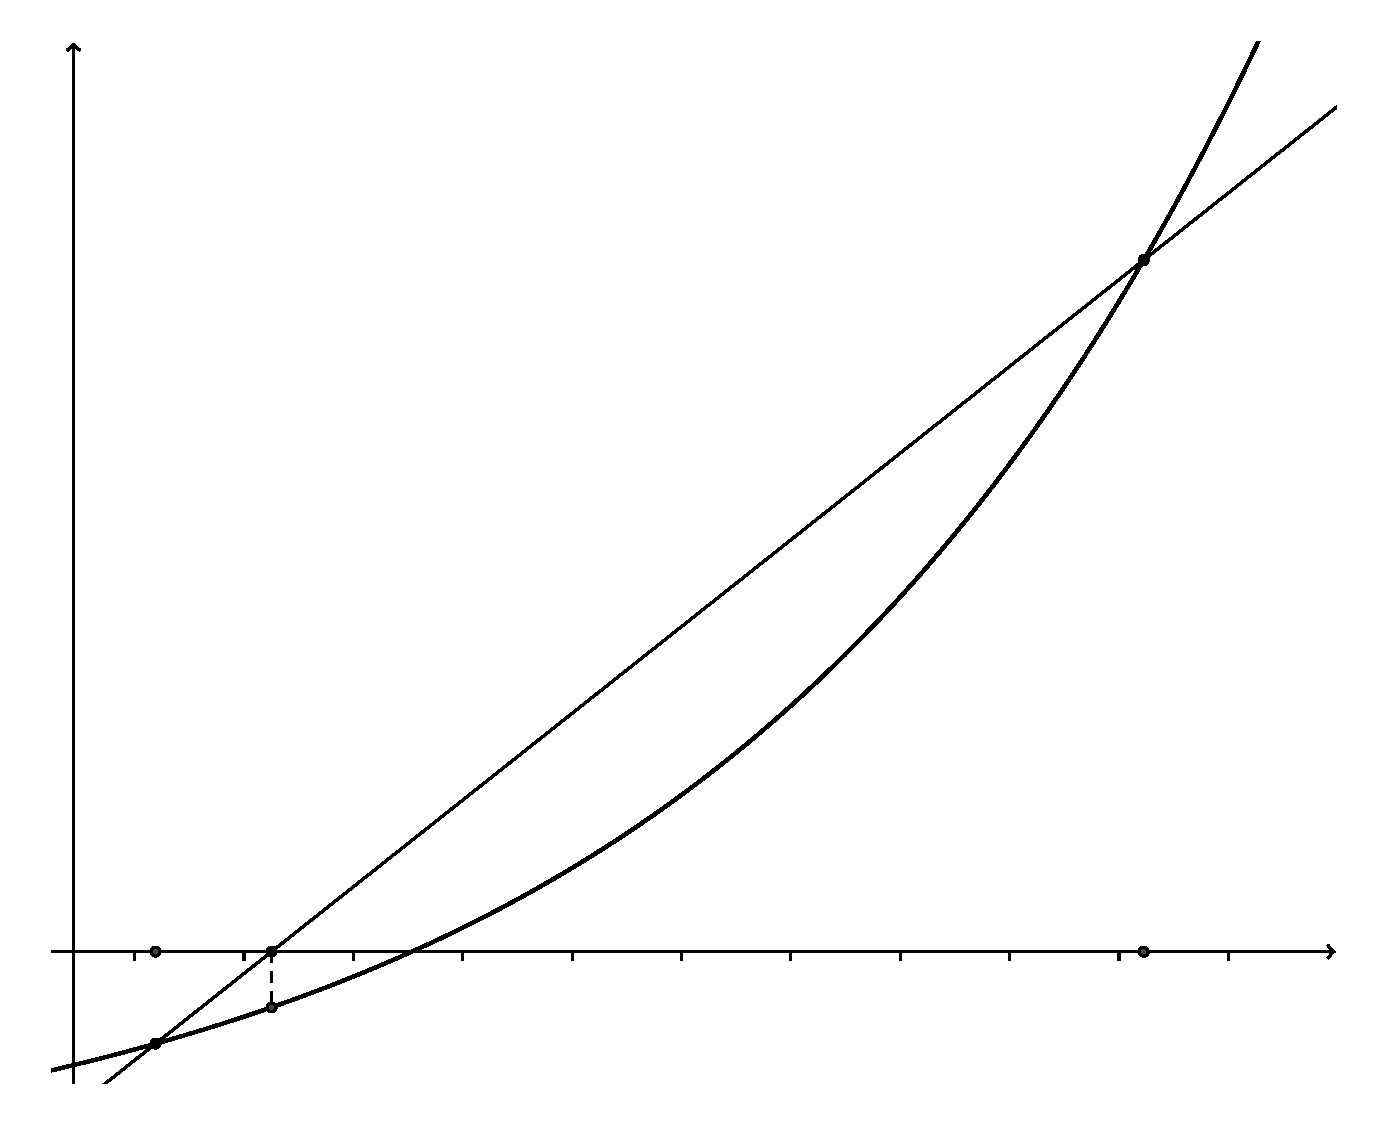
\includegraphics[width=0.6\textwidth]{figures/regula_falsi_secant.pdf}};
    \begin{scope}[x={(image.south east)},y={(image.north west)}]
        \node [right] at (0.6,0.4) {$f(x)$};
        \node [right] at (0.45,0.54) {$y(x)$};
        \node [right] at (0.8,0.73) {$f(c)$};
        \node [right] at (0.807,0.127) {$c$};
        \node [right] at (0.1,0.03) {$f(a)$};
        \node [right] at (0.092,0.127) {$a$};
        \node [right] at (0.16,0.188) {$b$};
    \end{scope}
\end{tikzpicture}
\caption{The secant line $y(x)$ is computed from the function $f(x)$ and a bracket $[a,c]_f$. $y(x) = 0$ is solved for the new update $b$ and used in the regula falsi method.}
\label{fig:regula_falsi_secant}
\end{figure}
\begin{algorithm}[ht]
 \SetAlgoLined
 \SetKw{And}{and}
 \KwData{Initial guess $x_i$, a bracket $[x_0,x_1]_f$ for the function $f(x)$, a tolerance $\epsilon$, and the iteration limit $n_{\text{max}}$}
 \KwResult{An approximate root of $f(x)$}
 $f_0 \coloneqq f(x_0)$\;
  $f_1 \coloneqq f(x_1)$\;
 \lIf{$x_i$ is a root}{\Return $x_0$}
 \lElse{Form a new bracket $[x_0,x_1]_f$ from $x_0$,$x_1$,$x_i$}
 \While{not converged \And iterations less than $n_{\text{max}}$}{
        \lIf{$[x_0,x_1]$ does not bracket the root}{handle the bracket error}
	$x_{n} \coloneqq \frac{x_1 f_0 - x_0 f_1}{f_0 - f_1}$\;
	$f_n \coloneqq f(x_n)$\;
	\lIf{$|f_n| < \epsilon$}{\Return $x_n$}
	\uIf{$f_n*f_0 < 0$}{
		$x_0 \coloneqq x_1$\;
		$f_0 \coloneqq f_1$\;
	}
	\Else{
	         $\gamma \coloneqq \frac{f_1}{f_1+f_n}$\;
	         $f_0 \coloneqq \gamma f_0$\;
	}
	$x_1 = x_n$\;
	$f_1 = f_n$\;
 }
 \Return the root approximation $\frac{x_0+x_1}{2}$
 \caption{Pseudo code implementing the Regula Falsi root finder, see Section \ref{section:regula_falsi}. The algorithm is modified with the \emph{Pegasus method}, due to \citet{dowell_the_1972}.}
\label{algorithm:regula_falsi}
\end{algorithm}
%%%%%%%%%%%%%%% RIDDER'S %%%%%%%%%%%%%%%%%
\subsubsection{Ridders' Method}
\label{section:ridders_method}
Ridders' method is another bracketing scheme, introduced by \citet{ridders_new_1979}. Again a bracket $[a,c]_f$ is chosen. A function $h(x)$ is defined by
\begin{equation*}
h(x) = f(x)\exp{\alpha x}.
\end{equation*}
Computing the midpoint $b$ of the bracket we want to find an $\alpha \in \mathbb{R}$ such that
\begin{equation*}
h(c) - 2h(b) + h(a) = 0.
\end{equation*}
Inserting $h(x)$ gives the following equation in $\alpha$:
\begin{equation*}
\exp{\alpha c}f_c - 2\exp{\alpha b}f_b + \exp{\alpha a}f_a = 0.
\end{equation*}
Multiplying this equation by $\exp{-\alpha a}$ gives
\begin{equation*}
\exp{\alpha (c-a)}f_c - 2\exp{\alpha (b-a)}f_b + \exp{\alpha (a-a)}f_a = \exp{\alpha 2\delta}f_c - 2\exp{\alpha \delta}f_b + f_a = 0,
\end{equation*}
since $c-a = 2(b-a)$ and $\delta \coloneqq b - a$. Thus we get a second order equation in $\exp{\alpha \delta}$. The solution of this equation can be found by 
\begin{equation} \label{eq:ridders_exp_sol}
\exp{\alpha \delta} = \frac{f_b \pm \sqrt{f_b^2 -  f_cf_a}}{f_c}.
\end{equation}
We now need to know under which restrictions this equation has a solution. Since $\exp{x} \geq 1,~\forall x \in \mathbb{R}$, we need the right hand side positive in order for the equation to have a solution. Definition \ref{definition:bracket} implies that $f_b^2 - f_cf_a \geq f_b^2 \geq 0$ and thus the square root always yields a real number. Since the square root is a monotonic and increasing function, this implies that $\sqrt{f_b^2 -  f_cf_a} \geq \vert f_b \vert$. Thus,
\begin{align*}
f_b + \sqrt{f_b^2 -  f_cf_a} &\geq 0, \nonumber \\
f_b - \sqrt{f_b^2 -  f_cf_a} &\leq 0 \nonumber,
\end{align*}
implying that the sign of the right hand side of Equation (\ref{eq:ridders_exp_sol}) is completely controlled by $\sgn{f_c}$. The solution $\exp{\alpha \delta}$ is then found by
\begin{equation} \label{eq:ridders_exp_sol_sgn}
\exp{\alpha \delta} = \frac{f_b + \sgn{f_c} \sqrt{f_b^2 -  f_cf_a}}{f_c} \coloneqq \sigma_{\alpha}.
\end{equation}
Now we find $\alpha$ by
\begin{equation*}
\alpha = \frac{\ln{\sigma_{\alpha}}}{\delta}.
\end{equation*}
Ridder's method proceeds by applying the Regula Falsi to $h(x)$ on the bracket $[b,c]_h$, using the regula falsi step in Equation (\ref{eq:regula_falsi_update}). This computes a new point $d$ by 
\begin{equation*}
d = b - h(b)\frac{c-b}{h(c) - h(b)}.
\end{equation*}
Inserting the definition for $h(x)$ gives
\begin{equation*}
d = b - \exp{\alpha b}f_b \frac{c-b}{\exp{\alpha c} f_c - \exp{\alpha b} f_b} = b - \frac{\delta f_b}{\exp{\alpha{c-b}}f_c - f_b}.
\end{equation*}
By Equation (\ref{eq:ridders_exp_sol_sgn}) $\exp{\alpha \delta}f_c$ is given by
\begin{equation*}
\exp{\alpha \delta}f_c = f_b + \sgn{f_c} \sqrt{f_b^2 -  f_cf_a},
\end{equation*}
and because $\delta = c-b$, we get
\begin{equation*}
d = b - \frac{\delta f_b}{f_b + \sgn{f_c} \sqrt{f_b^2 -  f_cf_a} - f_b} = b - \frac{\delta f_b}{\sgn{f_c} \sqrt{f_b^2 -  f_cf_a}}.
\end{equation*}
Now, by Definition \ref{definition:bracket}, $\sgn{f_c} = -\sgn{f_a}$. Using $\sgn{x} \coloneqq \frac{x}{\sqrt{{x}^2}}$ we arrive at Ridders' method:
\begin{equation} \label{eq:ridders_method}
d = b + \frac{\delta f_b}{\frac{f_a}{f_a^2} \sqrt{f_b^2 -  f_cf_a}} = b + \frac{ \delta \frac{f_b}{f_a}}{\sqrt{\left(\frac{f_b}{f_a}\right)^2 -  \frac{f_c}{f_a}}}.
\end{equation}
The final step involves selecting the smallest new starting bracket $[a,c]_f$ from the points $\{a,b,c\}$ in combination with point $d$, keeping with Definition \ref{definition:bracket}. Now the process is restarted, and continues until a root is found, or the size of the bracket falls below a tolerance $\epsilon$. Algorithm \ref{algorithm:ridders} shows the \opm implementation of Ridders' method.
\begin{algorithm}[ht]
 \SetAlgoLined
 \SetKw{And}{and}
 \KwData{Initial guess $x_i$, a highly unlikely answer $x_{\text{invalid}}$, a bracket $[x_0,x_1]_f$ for the function $f(x)$, a tolerance $\epsilon$, and the iteration limit $n_{\text{max}}$}
 \KwResult{An approximate root of $f(x)$}
 \lIf{$x_0$,$x_1$, or $x_i$ is a root}{\Return the root}
 \lElse{Form a new bracket $[x_0,x_1]_f$ from $x_0$,$x_1$,$x_i$}
  $f_0 \coloneqq f(x_0)$\;
  $f_1 \coloneqq f(x_1)$\;
  $x_r \coloneqq x_{\text{invalid}}$\;
 \While{not converged \And iterations less than $n_{\text{max}}$}{
        $x_m \coloneqq \frac{x_0+x_1}{2}$\;
        $f_m \coloneqq f(x_m)$\;
        $s \coloneqq \sqrt{f_m^2-f_0*f_1}$\;
        \lIf{$s$ is zero}{\Return $x_r$}
        \uIf{$f_0 \geq f_1$}{
        		$x_r \coloneqq x_m + (x_m-x_0)\frac{f_m}{s}$\;
        }
        \Else{
		$x_r \coloneqq x_m - (x_m-x_0)\frac{f_m}{s}$\;
        }
        \lIf{$x_r$ is converged under $\epsilon$}{\Return $x_r$}
        Form a new bracket $[x_0,x_1]_f$ from $x_0$, $x_1$, $x_m$, and $x_r$\;
 }
Error: The iteration limit $n_{\text{max}}$ is exceeded\;
 \caption{Pseudo code implementing Ridders' method, see Section \ref{section:ridders_method}.}
\label{algorithm:ridders}
\end{algorithm}
%\begin{figure}[ht]
%\begin{subfigure}[b]{0.49\textwidth}
%\centering
%\begin{tikzpicture}
%    \node[anchor=south west,inner sep=0] (image) at (0,0) {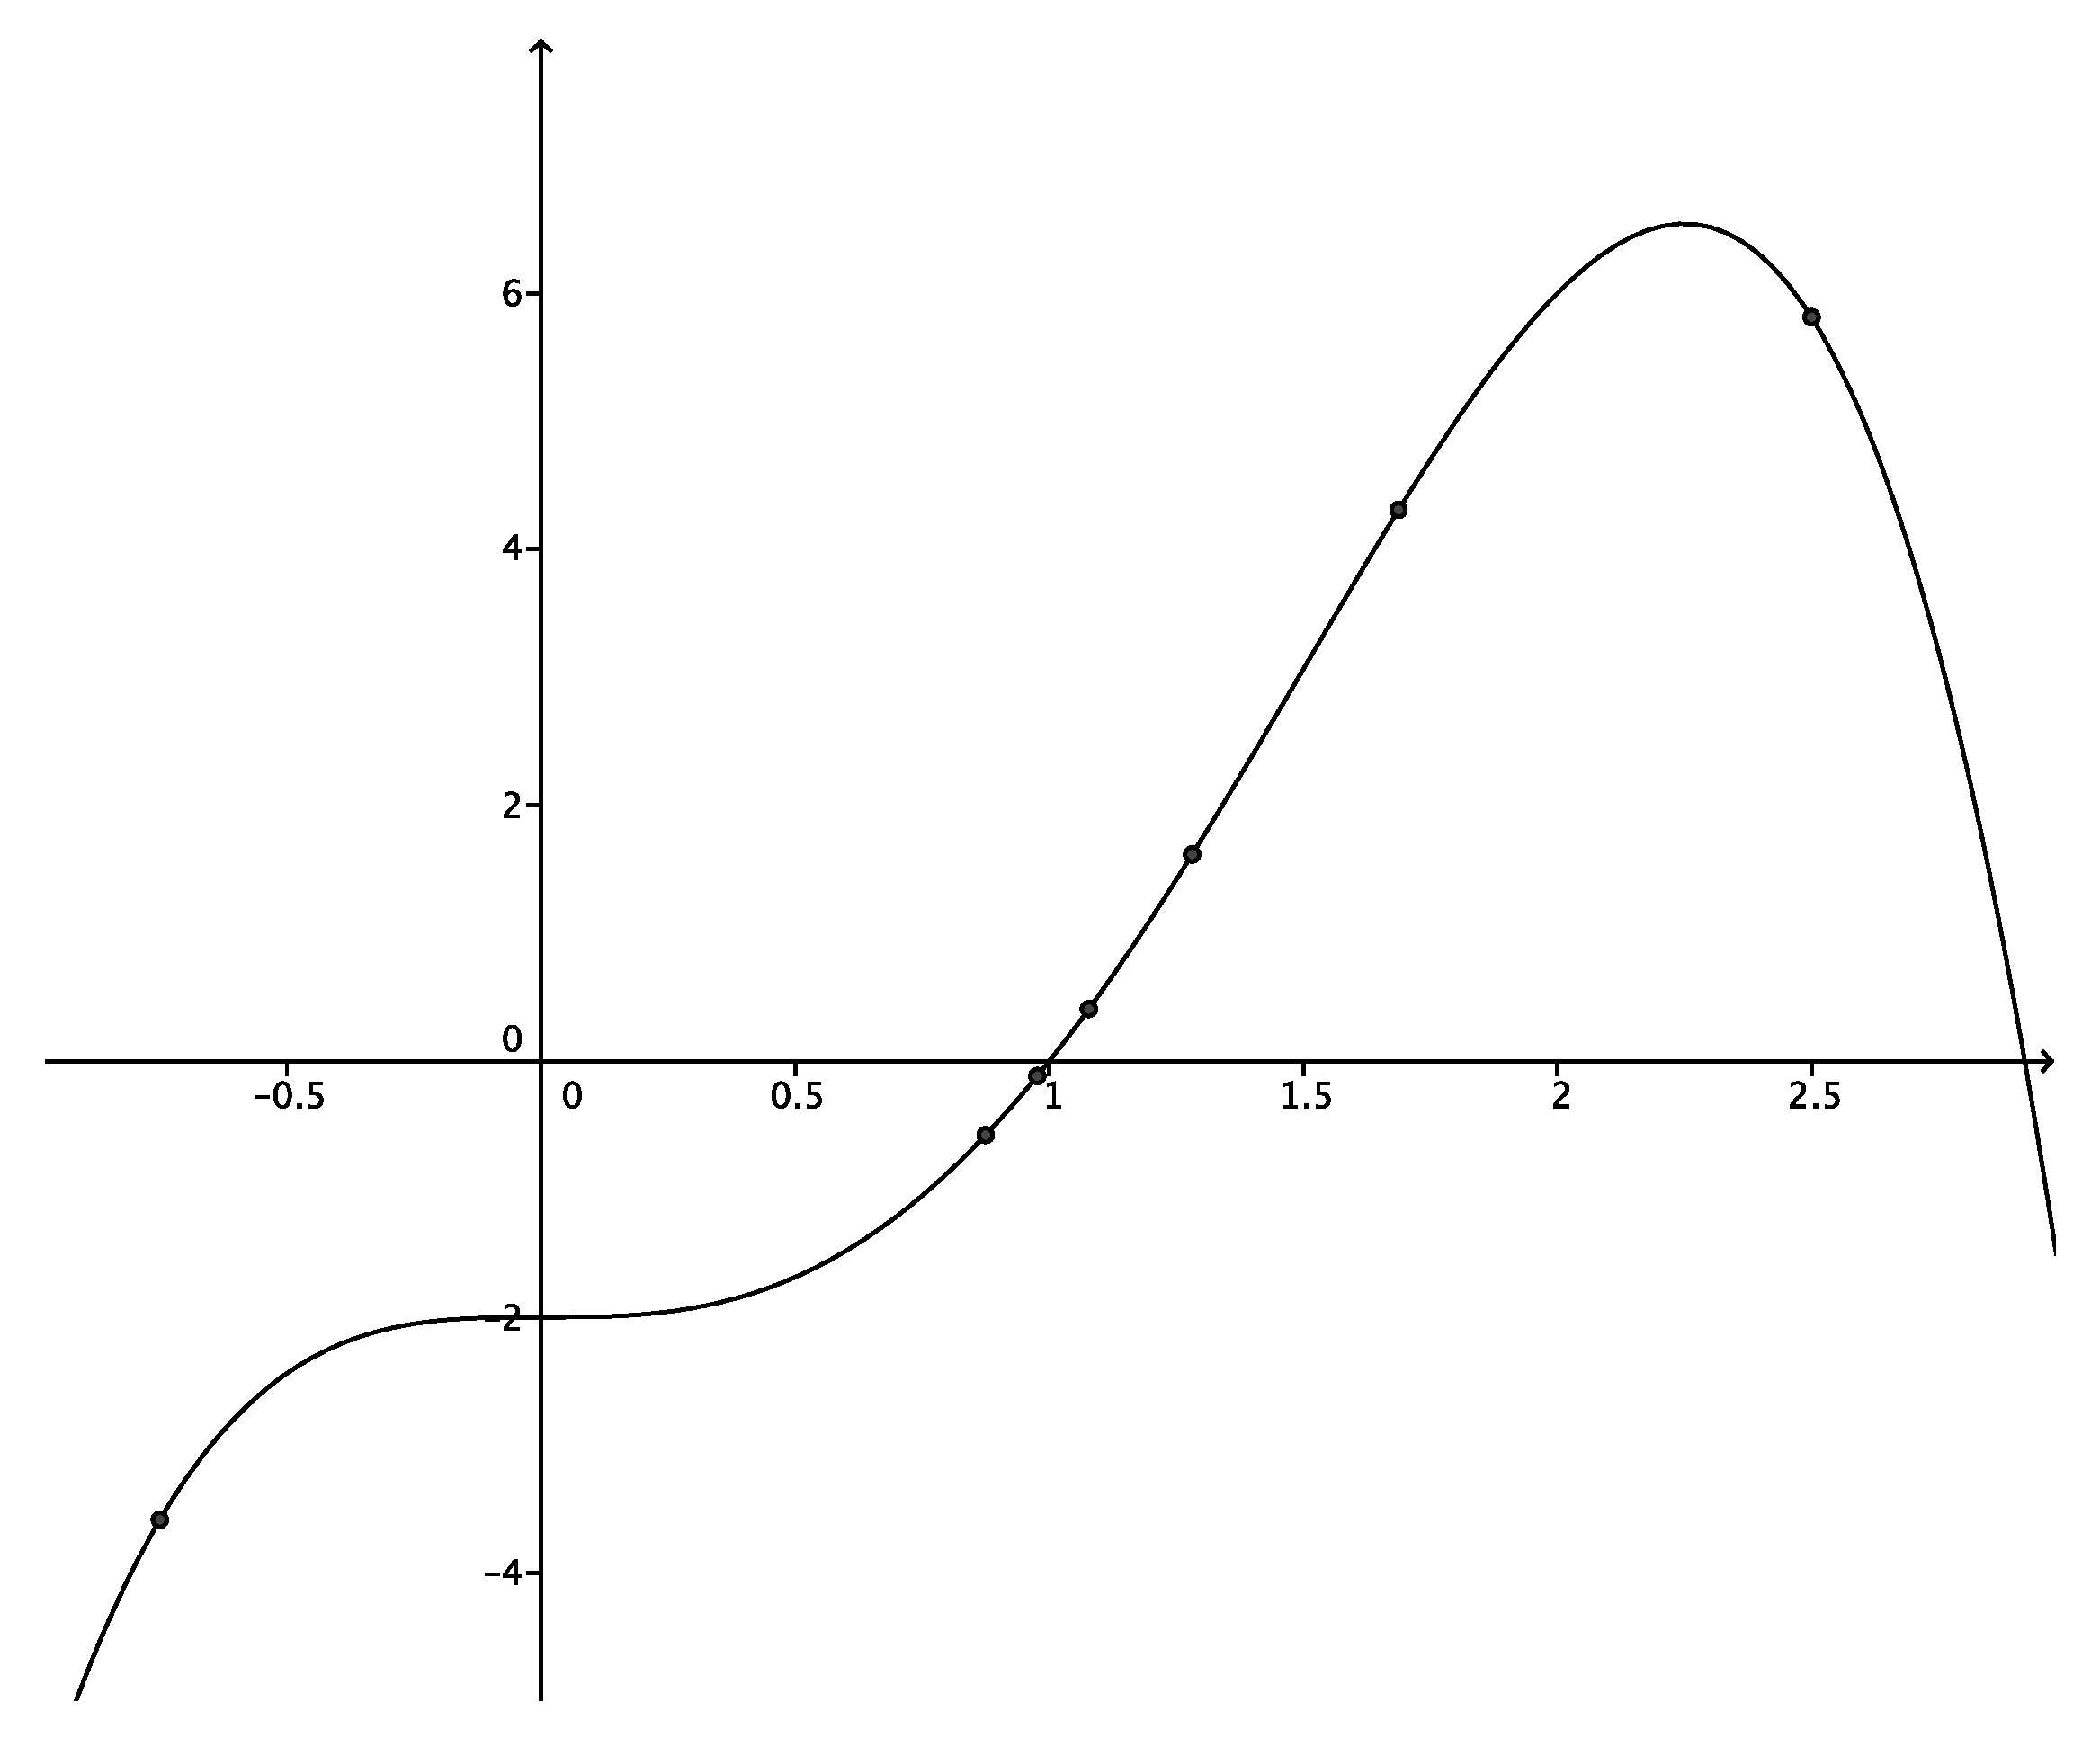
\includegraphics[width=0.9\textwidth]{figures/bisection.pdf}};
%    \begin{scope}[x={(image.south east)},y={(image.north west)}]
%        \node [right] at (0.08,0.1) {\scriptsize $a_0$};
%        \node [right] at (0.46,0.32) {\scriptsize $a_1 = b_0$};
%	\node [right] at (0.87,0.8) {\scriptsize $c_0$};
%
%        \node [right] at (0.66,0.69) {\scriptsize $c_2 = b_1$};
%        
%        \node [right] at (0.56,0.5) {\scriptsize $c_3 = b_2$};
%        
%        \node [right] at (0.52,0.42) {\scriptsize $c_4 = b_3$};
%        
%        \node [left] at (0.49,0.41) {\scriptsize $a_5 = b_4$};
%    \end{scope}
%\end{tikzpicture}
%\caption{Bisection} \label{fig:bisection}
%\end{subfigure}
%\begin{subfigure}[b]{0.49\textwidth}
%\centering
%\begin{tikzpicture}
%    \node[anchor=south west,inner sep=0] (image) at (0,0) {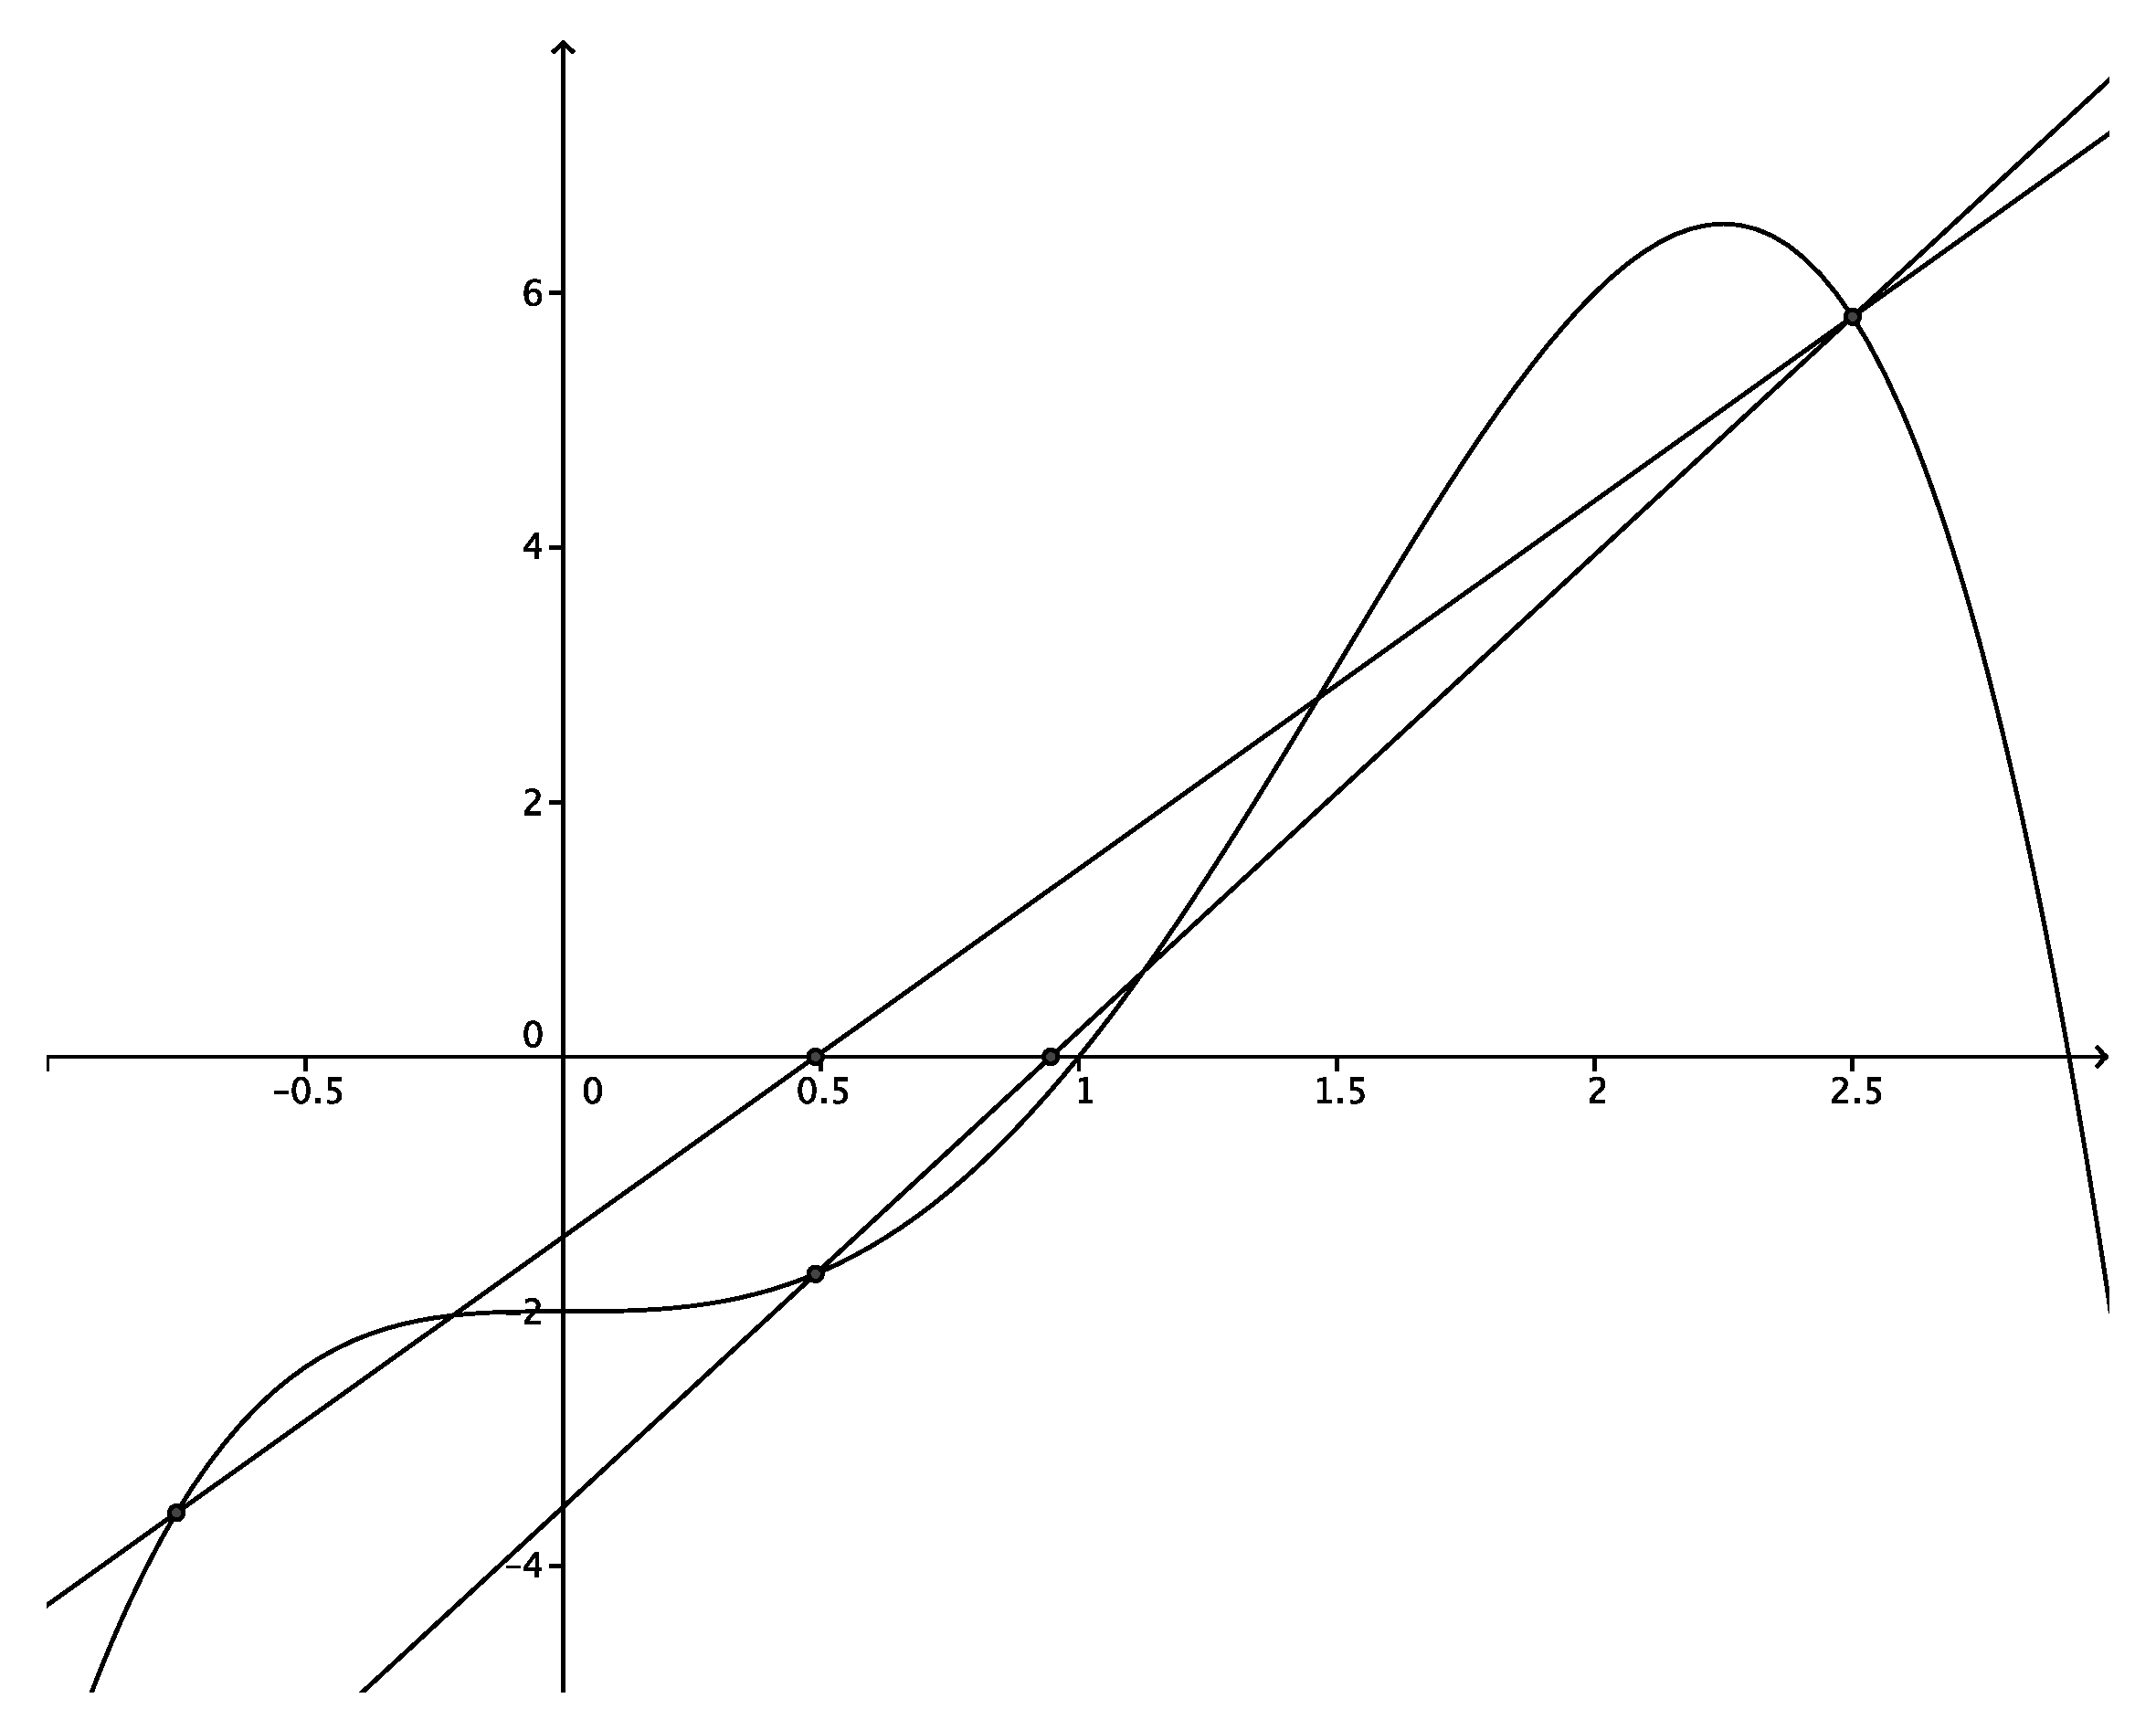
\includegraphics[width=0.9\textwidth]{figures/regula_falsi.pdf}};
%    \begin{scope}[x={(image.south east)},y={(image.north west)}]
%        \node [right] at (0.08,0.1) {\scriptsize $a_0$};
%        \node [right] at (0.36,0.25) {\scriptsize $a_1 = b_0$};
%	\node [right] at (0.87,0.8) {\scriptsize $c_0$};
%
%        \node [right] at (0.47,0.35) {\scriptsize $a_2 = b_1$};
%    \end{scope}
%\end{tikzpicture}
%\caption{Regula falsi}
%\label{fig:regula_falsi}
%\end{subfigure}
%\caption{Regula falsi and the bisection method solving $f(x) = -x^4 + 3x^3 - 2 = 0$.}
%\end{figure}

%\begin{figure}[ht]
%\begin{subfigure}[b]{0.49\textwidth}
%\centering
%\begin{tikzpicture}
%    \node[anchor=south west,inner sep=0] (image) at (0,0) {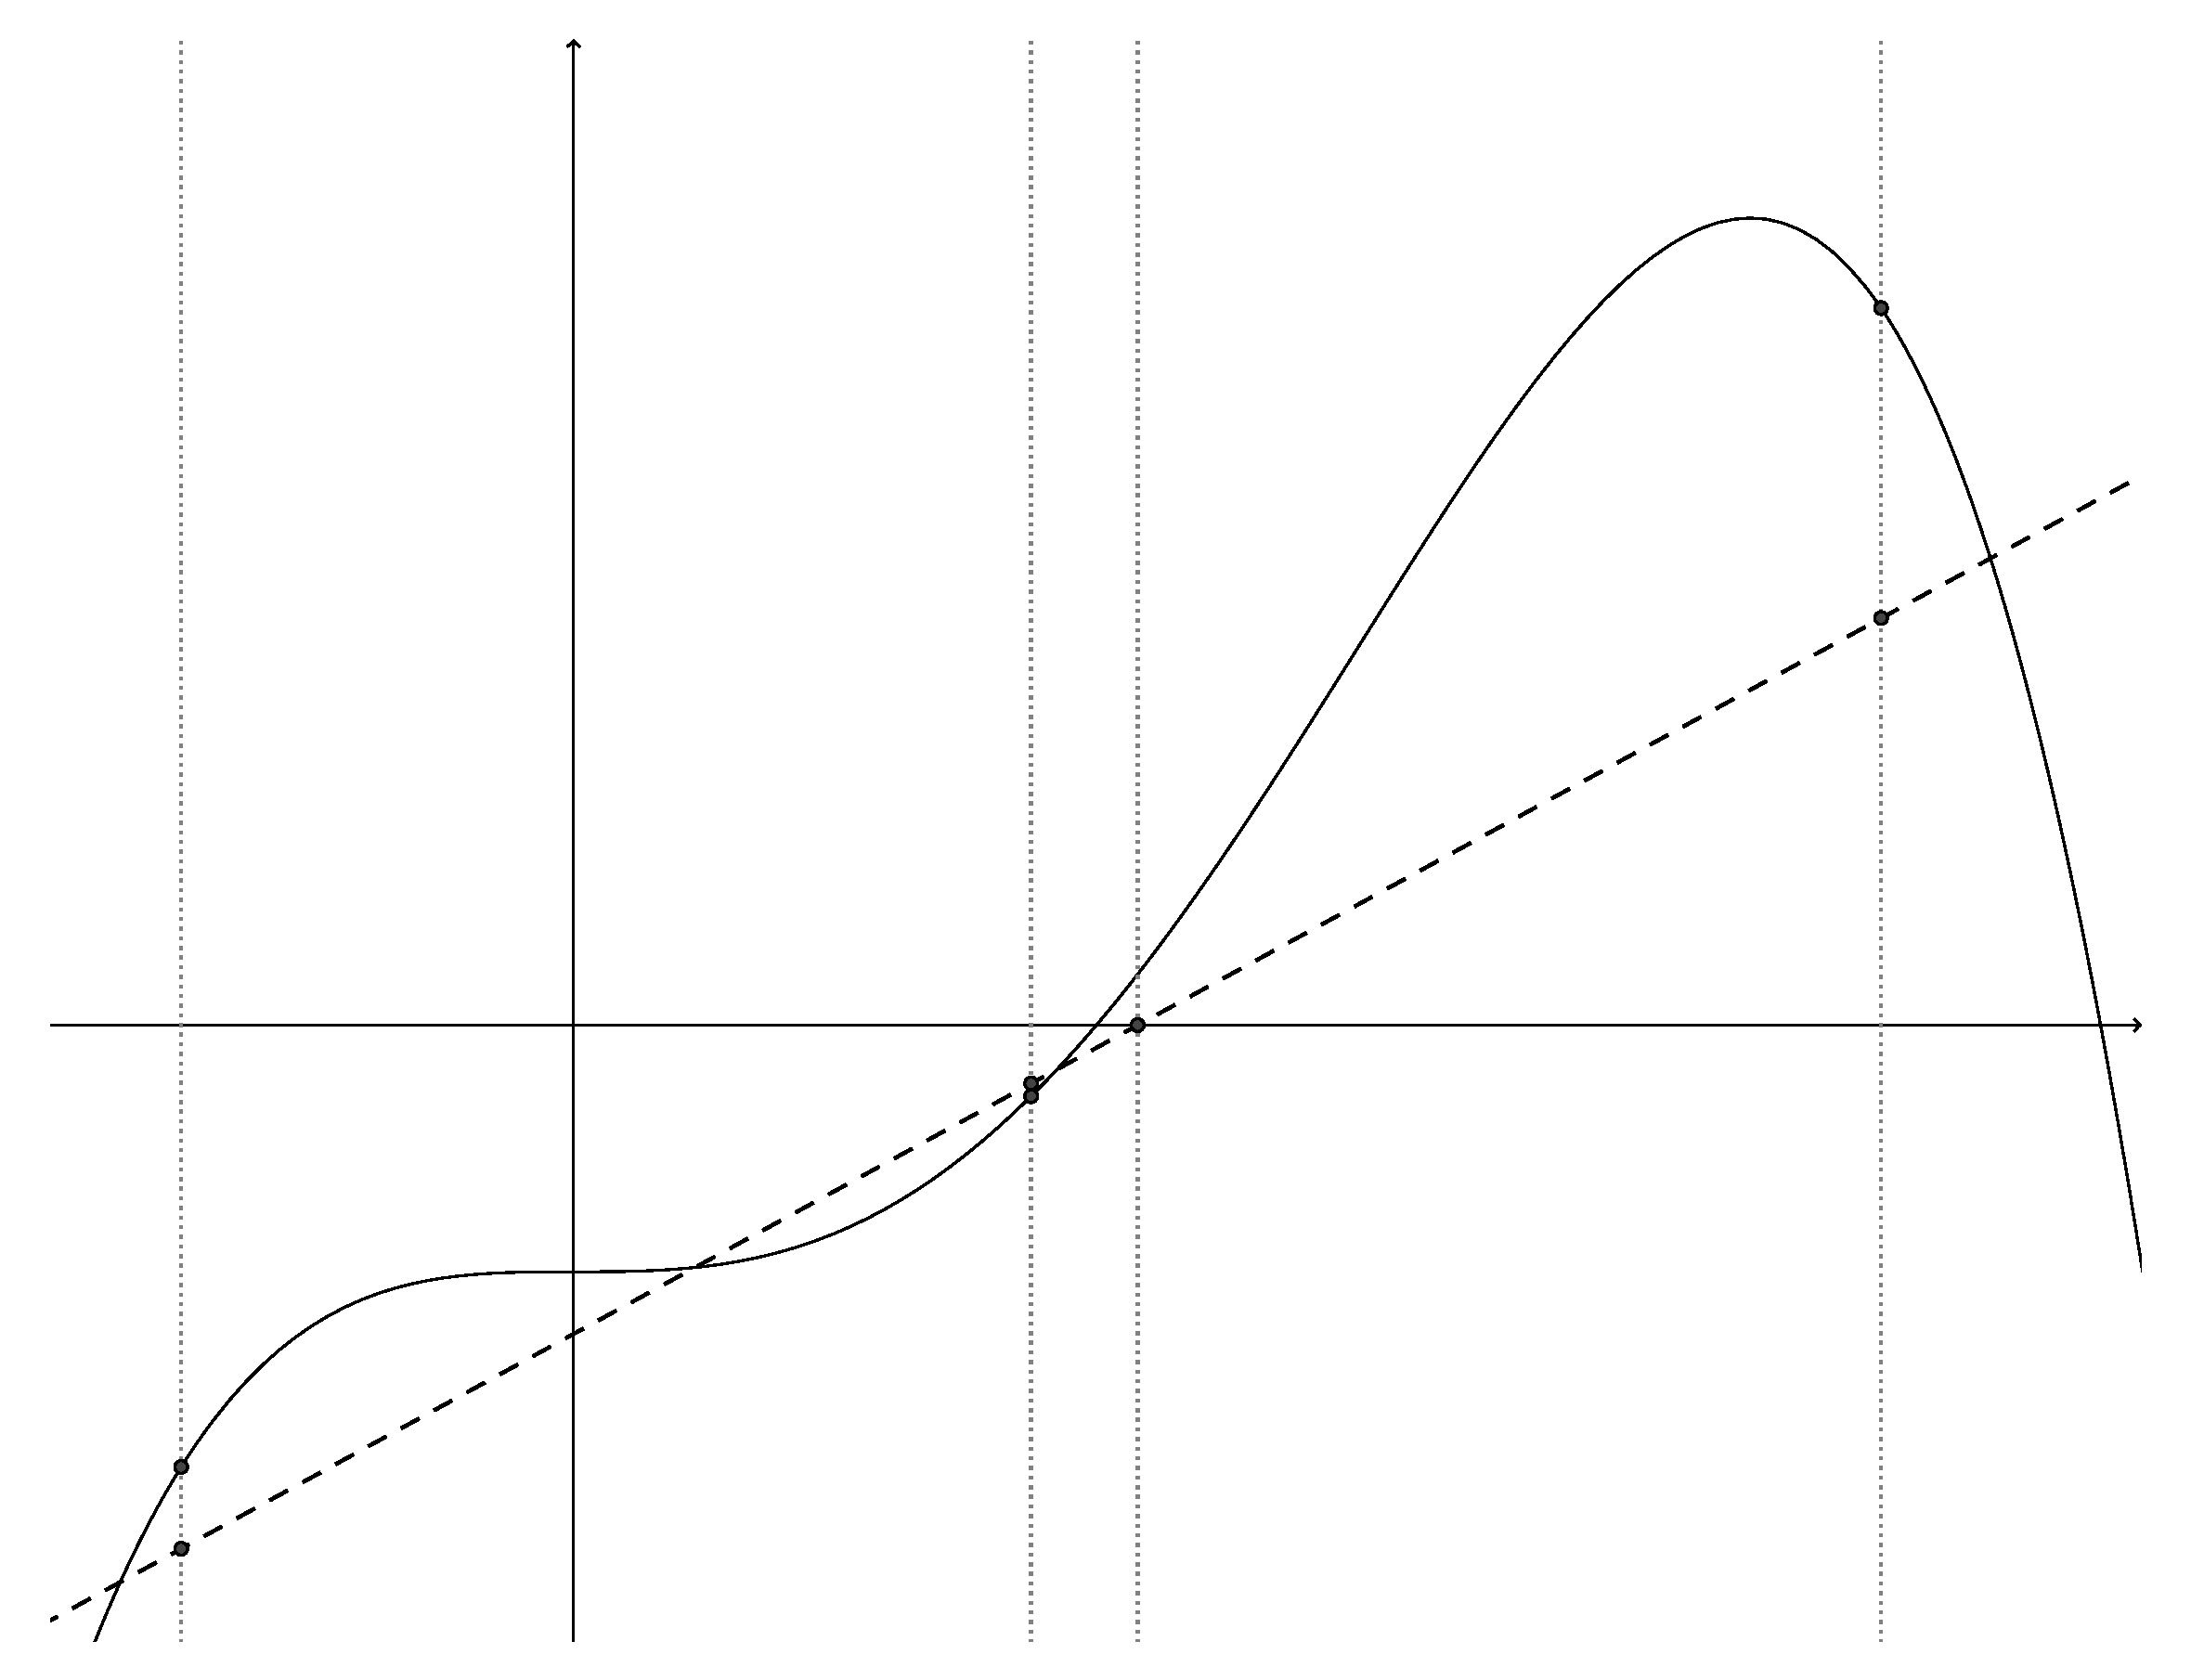
\includegraphics[width=0.9\textwidth]{figures/ridders_first_iteration.pdf}};
%    \begin{scope}[x={(image.south east)},y={(image.north west)}]
%        \node [right] at (0.07,0.06) {\scriptsize $a_0$};
%        \node [right] at (0.453,0.31) {\scriptsize $b_0$};
%        \node [right] at (0.505,0.34) {\scriptsize $d_0$};
%        \node [right] at (0.85,0.8) {\scriptsize $c_0$};
%    \end{scope}
%\end{tikzpicture}
%\caption{First iteration} \label{fig:ridders_first_iteration}
%\end{subfigure}
%\begin{subfigure}[b]{0.49\textwidth}
%\centering
%\begin{tikzpicture}
%    \node[anchor=south west,inner sep=0] (image) at (0,0) {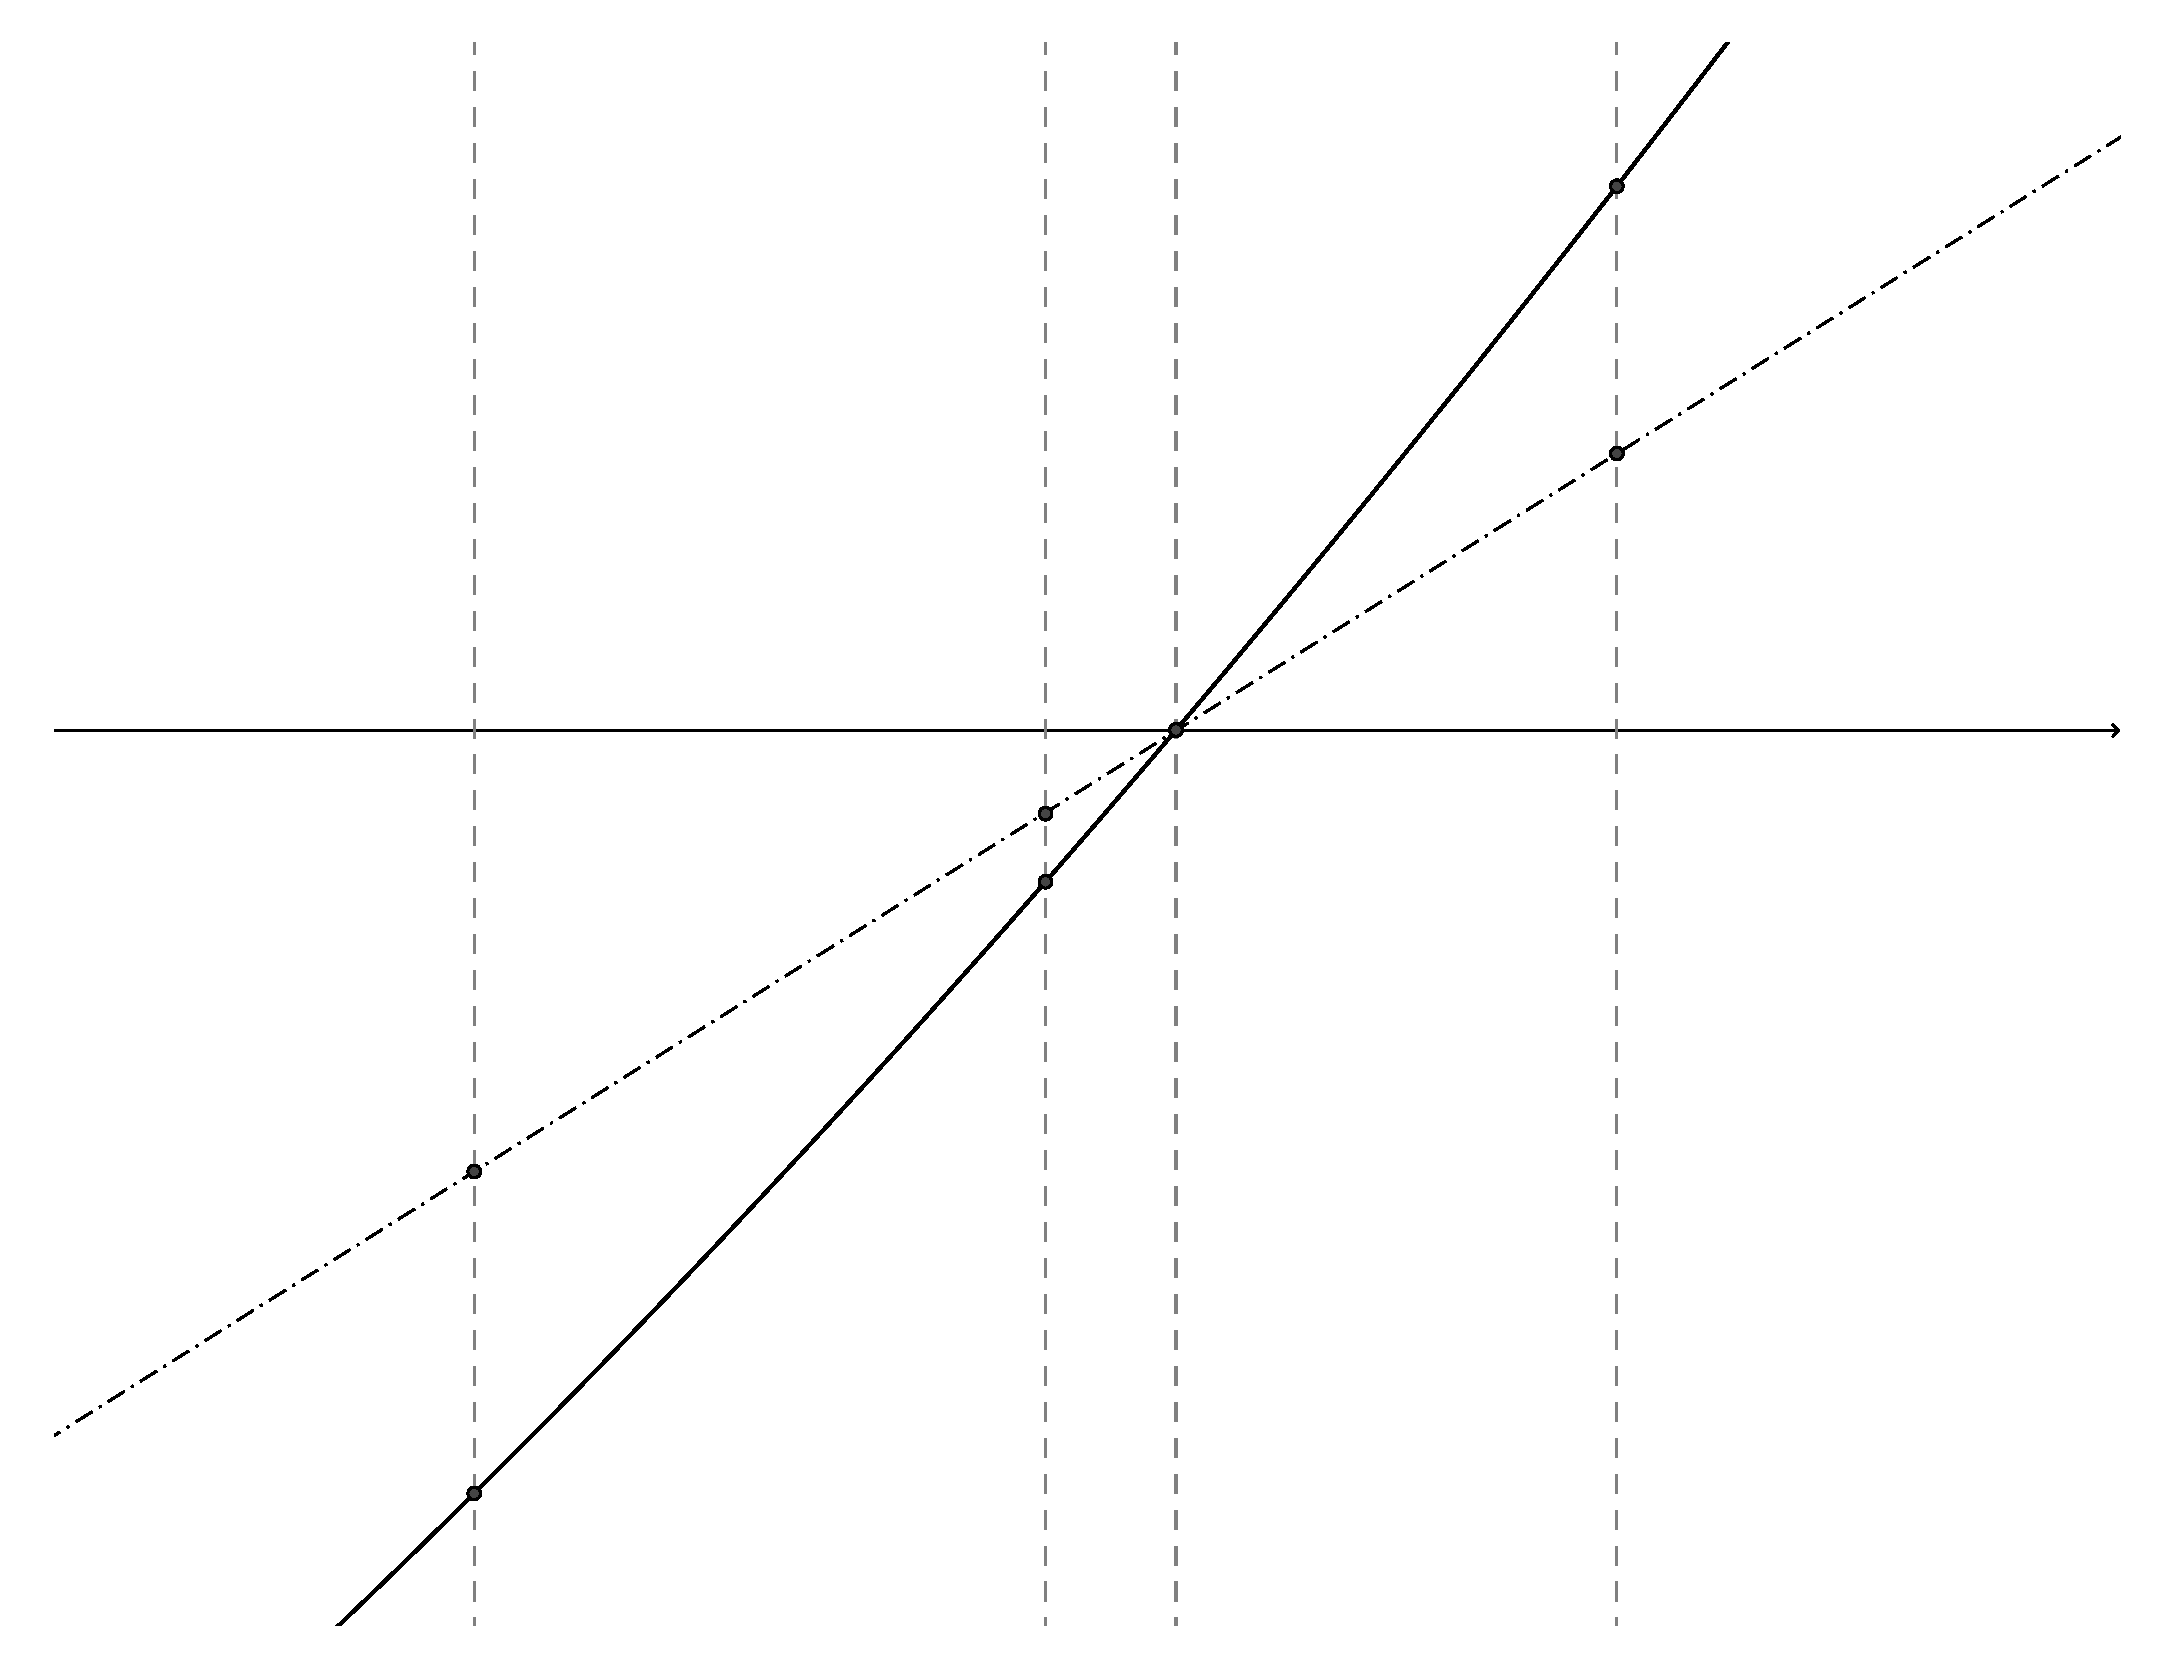
\includegraphics[width=0.9\textwidth]{figures/ridders_second_iteration_zoom.pdf}};
%    \begin{scope}[x={(image.south east)},y={(image.north west)}]
%        \node [right] at (0.22,0.08) {\scriptsize $a_1$};
%        \node [right] at (0.47,0.45) {\scriptsize $b_1$};
%        \node [right] at (0.53,0.53) {\scriptsize $d_1$};
%        \node [right] at (0.75,0.7) {\scriptsize $c_1$};
%    \end{scope}
%\end{tikzpicture}
%\caption{Second iteration, enlarged} \label{fig:ridders_second_iteration}
%\end{subfigure}
%\caption{Two iterations of Ridder's method solving $f(x) = -x^4 + 3x^3 - 2 = 0$. The initial bracket is $[-0.75,2.5]$. The midpoint $b_0$ and the root $d_0$ of the dashed $h(x)$ secant line  is chosen as bracket for the new iteration, i.e. $[a_1,c_1]  \coloneqq [b_0,d_0]$.} \label{fig:ridders}
%\end{figure}

%%%%%%%%%%%%%% BRENT'S METHOD %%%%%%%%%%%%%%%%%%
\subsubsection{Brent's Method} 
\label{section:brents_method}
Brent's method, due to \citet{brent_algorithms_1973}, combines the bisection method, see Section \ref{section:bisection_method}, the secant method, see Section \ref{section:secant_method} and \emph{inverse quadratic interpolation} and switches between the methods using a suitable heuristic. Brent's method is inspired by the older Dekker's method, see \citep{dekker_finding_1969}. We begin with a short presentation of inverse quadratic interpolation. 

Linear interpolation is used in for example the secant method (Section \ref{section:secant_method}) to approximate the function $f'(x)$ at two points $a,b$. Quadratic interpolation approximates $f(x)$ as a quadratic function, based on \emph{three} points $a,b,c$, possibly leading to complex roots. Similarly, inverse quadratic interpolation approximates $f^{-1}(y)$ by three points $f(a),f(b),f(c)$, that is
\begin{equation}
\label{eq:inverse_quadratic_interpolation}
f_*^{-1}(y) = \sum\limits_{i = 1}^3 f^{-1}(f_i) \prod\limits_{ \substack{j = 1 \\ j \neq i}}^3 \frac{y - f_j}{f_i - f_j}.
\end{equation}
Here $f_*^{-1}(y)$ denotes the interpolated function. Note that $f_i \coloneqq f(x_i)$, where $\ (x_1,x_2,x_3) \coloneqq (a,b,c,)$.The interpolated root is found by inserting $f(x_r) = 0$ into Equation (\ref{eq:inverse_quadratic_interpolation}). Since, by definition, $f^{-1}(f(x_r)) = x_r$ this gives an approximation for the root $x_r$ by the following equation (note the definition of an inverse quadratic interpolation function $\ell_{\text{iqi}}$):
\begin{equation}
\label{eq:inverse_quadratic_interpolation_root}
x_r \approx \sum\limits_{i = 1}^3 x_i \prod\limits_{ \substack{j = 1 \\ j \neq i}}^3 \frac{f_j}{f_i - f_j} \eqqcolon \ell_{\text{iqi}}(x_1,x_2,x_3).
\end{equation}

Brent's method starts with two points $a_k,b_k$ such that $f(a_k)f(b_k) < 0$ where $b_k$ is the current solution guess and $\vert f(a_k) \vert > \vert f(b_k) \vert$. At the initial step $k = 0$, we define $b_{-1} \coloneqq a_0$. A candidate update $s$ is found by
\begin{equation}
s = 
\begin{cases}
\ell_\text{iqi}(a_k,b_k,b_{k-1}),& \text{if $f(a_k) \neq f(b_{k-1})$ and $f(a_k) \neq f(b_{k-1})$}. \\
\ell_\text{s}(a_k,b_k),& \text{otherwise}.
\end{cases}
\end{equation}
The function $\ell_\text{s}$ implements the \emph{secant method} defined in Equation (\ref{eq:secant_method}). If $s \notin [\frac{3a_k+b_k}{4},b_k]$ a bisection step $s = \frac{a_k+b_k}{2}$ is used in this iteration. On the other hand, if $s \in [\frac{3a_k+b_k}{4},b_k]$ we define a number $\Delta$ such that
\begin{equation}
\Delta =
\begin{cases}
b_k - b_{k-1},& \text{if bisection was used in the previous iteration} \\
b_{k-1} - b_{k-2},& \text{if interpolation was used in the previous iteration}
\end{cases}
\end{equation}
Now, if $|s-b_k| \geq \frac{1}{2}\Delta$ or $\vert \Delta \vert \geq \delta$, for some tolerance $\delta > 0$, we fall back to the bisection method, such that $s = \frac{a_k+b_k}{2}$. If $f(a_k)f(s) < 0$, $b_{k+1} = s$ and $a_{k+1} = a_k$. If $f(a_k)f(s) \geq 0$, then $a_{k+1} = s$ and $b_{k+1} = b_k$. The final step is to ensure $|f(a_{k+1})| > |f(b_{k+1})|$ by swapping $a_{k+1}$ and $b_{k+1}$, if necessary. This iteration continues until the interval size is below a given tolerance $\epsilon$ or a root is found. Brent's method is shown in pseudo code in Algorithm \ref{algorithm:brents_method} following the implementation in the \opm code.
%\begin{algorithm}[ht]
% \SetAlgoLined
% \SetKw{And}{and}
% \KwData{Initial guess $x_i$, a bracket $[x_0,x_1]_f$ for the function $f(x)$, a tolerance $\epsilon$, the machine precision $\delta$, and the iteration limit $n_{\text{max}}$}
% \KwResult{An approximate root of $f(x)$}
% \lIf{$x_0$,$x_1$, or $x_i$ is a root}{\Return the root}
% \lElse{form a new bracket $[x_0,x_1]_f$ from $x_0$,$x_1$,$x_i$}
%  $f_0 \coloneqq f(x_0)$\;
%  $f_1 \coloneqq f(x_1)$\;
%  $f_2 \coloneqq f_1$\;
% \While{not converged \And iterations less than $n_{\text{max}}$}{
%	\lIf{$[x_1,x_2]_f$ is not a valid bracket}{define a new bracket $[x_1,x_2]$ with $|f_1| < |f_2|$ from points $x_0$ and $x_1$}
%	$x_m = \frac{x_2-x_1}{2}$\;
%	define a modified tolerance by $\epsilon_{\text{mod}} \coloneqq 2.0\delta|x_1| + 0.5\epsilon$\;
%	\lIf{If the solution $x_m$ is converged under $\epsilon_{\text{mod}}$}{\Return $x_1$}
%	\uIf{$|e| < \epsilon_{\text{mod}}$ \And $|f_0|>|f_1|$}{
%		Use inverse quadratic interpolation to find an update $d$\;
%		\lIf{the interpolation failed}{use a bisection step to find $d$}
%	}
%	\Else{
%		The interval bounds are decreasing too slowly: Use bisection to find an update $d$\;
%	}
%	Make a new bracket $[a,b]_f$\;
%	$f_b \coloneqq f(b)$\;
%}
%Error: The iteration limit $n_{\text{max}}$ is exceeded\;
% \caption{Pseudo code implementing Brent's method, see Section \ref{section:brents_method}.}
%\label{algorithm:brents_method}
%\end{algorithm}
\begin{algorithm}[ht]
 \SetAlgoLined
 \SetKw{And}{and}
  \SetKw{Or}{or}
 \KwData{Initial guess $x_i$, function $f(x)$, bracket $[x_0,x_1]_f$, tolerance $\epsilon$, iteration limit $n_{\text{max}}$}
 \KwResult{An approximate root of $f(x)$}
 \lIf{$x_0$,$x_1$, or $x_i$ is a root}{\Return the root}
 \lElse{form a new bracket $[x_0,x_1]_f$ from $x_0$,$x_1$,$x_i$}
  $f_0 \coloneqq f(x_0)$\;
  $f_1 \coloneqq f(x_1)$\;
 \While{not converged \And iterations less than $n_{\text{max}}$}{
	use inverse quadratic interpolation to find an update $x_n$\;
	\lIf{the interpolation failed}{use the secant method to find $x_n$}
	\lIf{iterate $x_n$ converged to slowly}{do a bisection step on $x_n$}
	form a new bracket from points $x_0,x_1,x_n$\;
}
\lIf{point $x_1$ or $x_n$ is a converged root}{\Return $x_1$ or $x_n$}
\lElse{the iteration limit $n_{\text{max}}$ is exceeded}
\caption{Pseudo code implementing Brent's method, see Section \ref{section:brents_method}.}
\label{algorithm:brents_method}
\end{algorithm}

%%%%%%%%%%%%% NEWTON'S METHOD %%%%%%%%%%%%%%%%%%%
\subsubsection{Newton's Method}
\label{section:newtons_method}
Unlike the bisection method, Regula Falsi, and Ridders' method, Newton's method is an \emph{open} method, meaning that it does not restrict the search to a closed interval. This important feature allows the iterates to take on any value $x \in \mathbb{R}$, opening up the possibility for divergence of the solution. The upside is that the method has quadratic local convergence, in contrast to the super-linear convergence of the previously mentioned methods \citep{kincaid_ch._2002}. Newton's method does not exhibit global convergence properties. 

To derive Newton's method for solving $f(x) = 0,~x\in\mathbb{R},f\colon\mathbb{R}\to\mathbb{R}$, we start with a Taylor expansion of $f(x)$ around an initial guess $x_0$:
\begin{equation*}
f(x) = f(x_0) + (x-x_0)f'(x_0) + \frac{(x-x_0)^2}{2!}f''(x_0) + \mathcal{O}((x-x_0)^3).
\end{equation*}
Evaluating this function at the root, say $x_r$, gives:
\begin{equation*}
f(x_r) = f(x_0) + \Delta x_0 f'(x_0) + \frac{\Delta x_0 ^2}{2!}f''(x_0) + \mathcal{O}(\Delta x_0^3) = 0,
\end{equation*}
where $\Delta x_0 = x-x_0$. Dropping all higher order terms in $\Delta x_0$ leads to the following approximate equation:
\begin{equation*}
0 = f(x_r) \approx f(x_0) + \Delta x_0 f'(x_0).
\end{equation*}
This relation implies that
\begin{equation*}
\Delta x_0 \approx -\frac{f(x_0)}{f'(x_0)} \implies x_r \approx x_0 - \frac{f(x_0)}{f'(x_0)} \coloneqq x_1.
\end{equation*}
for $f'(x_0) \neq 0$. Here $x_1$ is an updated guess for the root $x_r$. Iterating this equation leads to Newton's method for a univariate equation:
\begin{equation}
\label{eq:newtons_method}
x_{n+1} = x_n - \frac{f(x_n)}{f'(x_n)}. 
\end{equation}

Newton's method can also be derived from a geometric argument. The tangent $y(x;x_n)$ to a curve $f(x)$ at a point $x_n$ is given as
\begin{equation*}
y(x;x_n) = f'(x_n)(x-x_n)+f(x_n).
\end{equation*}
As long as $f'(x_n) \neq 0$ this tangent will cross the $x$-axis, i.e. we can find a root $x_{r_n}$ such that $y(x_{r_n};x_n) = 0$. The solution to this equation is given as
\begin{equation*}
x_{r_n} = x_n - \frac{f(x_n)}{f'(x_n)},
\end{equation*}
which when setting the new iterate $x_{n+1} = x_{r_n}$ is equivalent to Equation (\ref{eq:newtons_method}). Figure \ref{fig:newtons_method} illustrates the geometric interpretation and one step of Newton's method.
\tikzsetnextfilename{newton_tangent}
\begin{figure}[ht]
\centering
\begin{subfigure}[b]{0.49\textwidth}
\begin{tikzpicture}
    \node[anchor=south west,inner sep=0] (image) at (0,0) {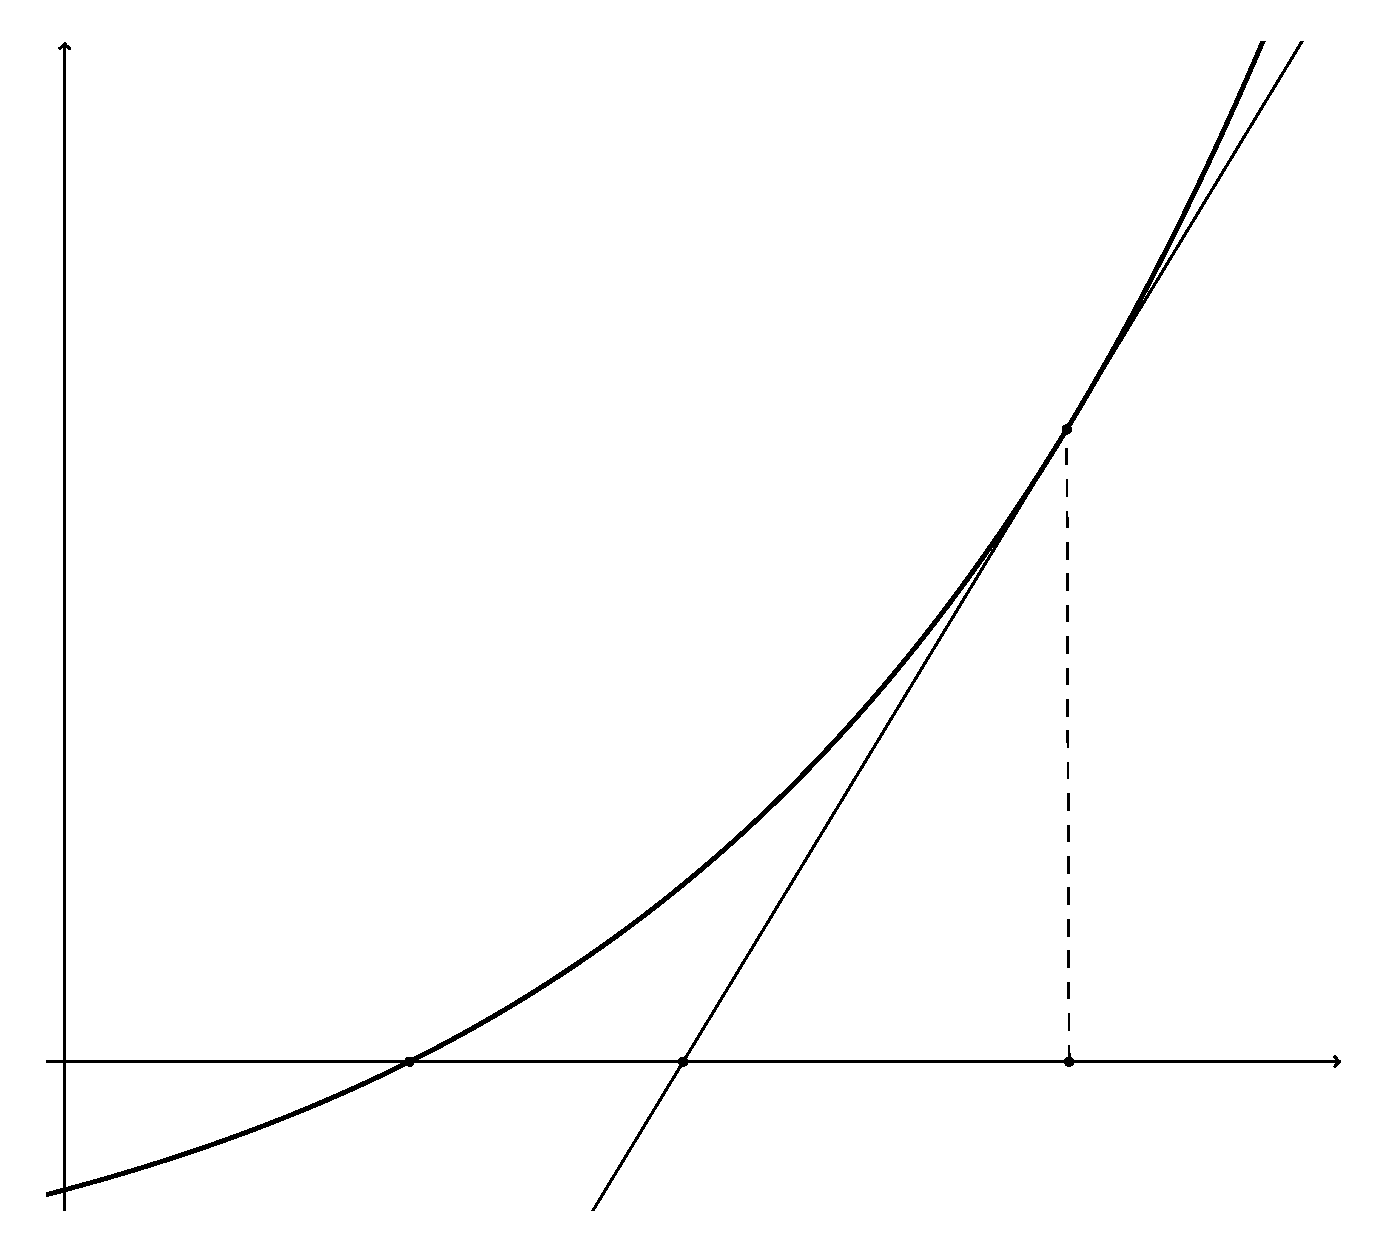
\includegraphics[width=1.0\textwidth]{figures/newtons_method_convergence.pdf}};
    \begin{scope}[x={(image.south east)},y={(image.north west)}]
        \node [right] at (0.3,0.3) {$f(x)$};
        \node [right] at (0.77,0.69) {$f(x_0)$};
        \node [right] at (0.78,0.1) {$x_0$};
        \node [right] at (0.47,0.1) {$x_1$};
        \node [right] at (0.24,0.1) {$x_r$};
        \node [right] at (0.56,0.25) {$y(x)$};
    \end{scope}
\end{tikzpicture}
\end{subfigure}
\caption{One step of Newton's method on the function $f(x)$ used to approximate the root $x_r$. The new iterate $x_1$ is found by computing the root of the tangent line $y(x)$ to $f(x)$ at the initial guess $x_0$.}
\label{fig:newtons_method}
\end{figure}
%%%%%%%%%%%% SECANT METHOD %%%%%%%%%%%%%%%%%%%%
\subsubsubsection{The Secant Method}
\label{section:secant_method}
The \emph{secant method} is a derivative free version of Newton's method obtained by approximating $f'(x_n)$ as
\begin{equation*}
f'(x_n) \approx \frac{ f(x_n) - f(x_{n-1}) }{ x_n - x_{n-1}}
\end{equation*}
Inserted into Equation (\ref{eq:newtons_method}) this yields
\begin{equation}
\label{eq:secant_method}
x_{n+1} = \ell_{\text{s}}(x_n,x_{n-1}) = x_n - f(x_n)\frac{ f(x_n) - f(x_{n-1}) }{ x_n - x_{n-1} } \eqqcolon \ell_{\text{s}}(x_n,x_{n-1}).
\end{equation}
Note that two initial guesses are required to start the method and that we have defined a secant method function $\ell_{\text{s}}$ for later use. The secant method has a super-linear convergence rate whereas Newton's method converges quadratically \citep{kincaid_ch._2002}.
%%%%%%%%%%%%%% TRUST REGIONS %%%%%%%%%%%%%%%%%%
\subsubsection{Trust Regions}
\label{section:trust_regions}
\todoinline{Explain how the inflection point is found for the trust region scheme}
As mentioned in Section \ref{section:newtons_method}, Newton's method can diverge for bad initial guesses. Despite this shortcoming we would like to exploit the nice convergence properties of the method. Several modifications have been proposed, among others the \emph{Appleyard Heuristic} and the \emph{Modified Appleyard Heuristic}, see e.g. \citep{younis_modern_2011}. These methods seeks to scale the Newton update $\frac{f(x_n)}{f'(x_n)}$ to stop the method from diverging or using too many iterations to converge. Since we want to solve Equation (\ref{eq:residual_two_phase_transport}) for the saturation $S_V^{n+1}$ we already have a well defined region of allowable values, namely $S_V^{n+1} \in [0,1]$. This fact obviously follows from the physics of the problem and allows us to limit the Newton updates to this interval, keeping the iterates from diverging. This is one example of an imposed heuristic. Another approach, used in optimization, is to define a region within which the iterative technique is trusted to compute valid results, a so called \emph{trust region}. \citet{jenny_unconditionally_2009} applies this to reservoir simulation residuals by identifying regions where the Newton method converges reliably. This can also be viewed as a globalization technique for Newton's method. In order to present the update scaling choices for the trust region methods we first introduce the \emph{dimensionless flux function}.
\begin{figure}[ht]
\tikzsetnextfilename{water_flux_viscosity}
\begin{subfigure}[b]{0.32\textwidth}
	\centering
    	\begin{tikzpicture} [scale=0.5]
	\begin{axis}[
		xlabel={$S$},
		ylabel={$F_w(S)$},
		xmin = 0,
		xmax = 1,
		ymin = 0,
		ymax = 1,
		domain = 0:1,
		samples = 100,
		grid = major
		]
	\addplot [mark=none, thick] {x^2/(x^2+0.1*(1-x)^2)};
	\addplot [black, mark = *, nodes near coords=$S_{\text{inflec}}$,every node near coord/.style={anchor=180}] coordinates {( 0.1859, 0.3427)};
	\end{axis}
	\end{tikzpicture}
	\caption{Viscosity} \label{fig:dimless_water_flux_viscosity}
\end{subfigure}
\tikzsetnextfilename{water_flux_buoyancy}
\begin{subfigure}[b]{0.32\textwidth}
	\centering
	\begin{tikzpicture} [scale=0.5]
	\begin{axis}[
		xlabel={$S$},
		ylabel={$F_w(S)$},
		xmin = 0,
		xmax = 1,
		ymin = 0,
		ymax = 1.2,
		domain = 0:1,
		samples = 100,
		grid = major
		]
	%\addplot [mark=none, thick] {(1-x)^2*x^2/(x^2+(1-x)^2) + (1-x)^2*x^2/(x^2+(1-x)^2)};
	%\addplot [black, mark = *, nodes near coords=$S_{\text{inflec}}$,every node near coord/.style={anchor=180}] coordinates {( 0.1325,0.1424)};
	%\addplot [black, mark = *, nodes near coords=$S_{\text{inflec}}$,every node near coord/.style={anchor=180}] coordinates {( 0.5278,0.2064)};
	%\addplot [black, mark = *, nodes near coords=$S_{\text{s}}$,every node near coord/.style={anchor=200}] coordinates {( 0.3170,0.3186)};
	\addplot [mark=none, thick] {x^2/(x^2+0.1*(1-x)^2) + (1-x)^2*x^2/(x^2+0.1*(1-x)^2)};
	\addplot [black, mark = *, nodes near coords=$S_{\text{inflec}}$,every node near coord/.style={anchor=180}] coordinates {( 0.160446,0.456081)};
	\addplot [black, mark = *, nodes near coords=$S_{\text{inflec}}$,every node near coord/.style={anchor=200}] coordinates {( 0.667646,1.083607)};
	\addplot [black, mark = *, nodes near coords=$S_{\text{s}}$,every node near coord/.style={anchor=90}] coordinates {(0.484458,1.137022)};
	\addplot [black, mark = *, nodes near coords=$S_{\text{f=1}}$,every node near coord/.style={anchor=330}] coordinates {(0.315,1.0)};
	\end{axis}
	\end{tikzpicture}
	\caption{Buoyancy} \label{fig:dimless_water_flux_buoyancy}
\end{subfigure}
\tikzsetnextfilename{water_flux_capillarity}
\begin{subfigure}[b]{0.32\textwidth}
	\centering
	\begin{tikzpicture} [scale=0.5]
	\begin{axis}[
		xlabel={$S$},
		ylabel={$F_w(S)$},
		xmin = 0,
		xmax = 1,
		ymin = 0,
		ymax = 1.5,
		domain = 0:1,
		samples = 100,
		grid = major
		]
	\addplot [mark=none, thick] {1.5*x^2/(x^2+0.1*(1-x)^2)};
	\addplot [black, mark = *, nodes near coords=$S_{\text{inflec}}$,every node near coord/.style={anchor=180}] coordinates {( 0.1859,0.5141)};
	\end{axis}
	\end{tikzpicture}
	\caption{Capillarity} \label{fig:dimless_water_flux_capillarity}
\end{subfigure}
\caption{Water flux function $F_w$ dominated by viscosity, buoyancy and capillarity. $S_{\text{inflec}}$ denotes inflection points and $S_{\text{s}}$ sonic points.}%
\label{fig:dimensionless_water_flux_function}%
\end{figure}%
%%%%%%%%%%%%%%%% DIM.LESS FLUX FUNCTION %%%%%%%%%%%%%%%%
\subsubsubsection{The Dimensionless Flux Function}
\citet{wang_trust-region_2013} defines a \emph{dimensionless water flux function} by
\begin{equation} \label{eq:water_flux_function}
F_w = \frac{u_w}{u} = f_w + \frac{K g \lambda_o f_w(\rho_w-\rho_o) \nabla h}{u_t} + \frac{f_w K \lambda_o \nabla p_c}{u_t}.
\end{equation}
Here the permeability and gravity are assumed to be scalar. This equation states the water flux as a product of three terms; the viscosity terms, the buoyancy term, and the capillarity term, in that order. The idea is that this function is the main contribution to the non-linearity of the transport residual, and that this fact can be used to develop efficient update heuristics for Newton's method \citep{jenny_unconditionally_2009}. Because the transport equation has been split into two equations, see Section \ref{section:transport_solver}, we operate with a slightly modified set of flux functions, the effects of which is most apparent in the buoyancy term. The flux functions for the three regimes are shown in Figure \ref{fig:dimensionless_water_flux_function}. It is apparent from the figure that the different regimes have qualitative differences, which will be exploited in two different trust region schemes.
\begin{algorithm}%
 \SetKw{And}{and}
 \SetAlgoLined
 \KwData{Initial guess $x_0$, function $f(x)$, tolerance $\epsilon$}
 \KwResult{A approximate root $x_r$}
 $x_n = x_0$\;
 \While{$f(x_n) > \epsilon$ \And $\Delta x_n > \epsilon$}{
 	$\Delta x_n \coloneqq \frac{f(x_n)}{f'(x_n)}$\;
	\If{$x_n + \Delta x_n$ has crossed an inflection point $x_{\text{inflec}}$}{
		$\Delta x_n \coloneqq x_{\text{inflec}} - x_n $\;
	}
	$x_n \coloneqq x_n + \Delta x_n$\;
 }
 $x_r \coloneqq x_n$\;
 \Return the root $x_r$
 \caption{Pseudo code implementing the JTR method, see Section \ref{section:numerical_methods_trust_region_jenny}.}%
\label{algorithm:jtr}%
\end{algorithm}%
%%%%%%%%%%%%% JENNY ET AL. %%%%%%%%%%%%%%%%%%%
\subsubsubsection{Jenny et al. Trust Region}
\label{section:numerical_methods_trust_region_jenny}
\citet{jenny_unconditionally_2009} presents an update heuristic for the Newton method in the viscosity dominated case, with the flux function shown in Figure \ref{fig:dimless_water_flux_viscosity}. This function is s-shaped and its qualitative features are governed by the fractional flow function $f_w$. A closer inspection of this function shows that the domain $[0,1]$ can be split into two subsets such that $F_w$ is concave on one and convex on the other. This is convenient, since Newton's method is known to converge regardless of starting point on convex or concave functions, see e.g. \citet{morris_computational_1983}. A smooth function making a transition from a concave to a convex region, or vice versa, must cross the so called \emph{inflection point}, here denoted $S_{\text{inflec}}$. The inflection point is exactly the point where the second derivative of the function at hand changes sign. The \emph{Jenny Trust Region} method, or the JTR, introduced in \citet{jenny_unconditionally_2009}, tries to exploit the convergence guarantee of the Newton-Raphson method on convex or concave regions by first doing a regular Newton solve and then restricting the saturation such that no update leaps between the two regions. That is, if a saturation update $\Delta S$ and the initial saturation $S$ is such that $(S-S_{\text{inflec}})(S+\Delta S - S_{\text{inflec}}) < 0$, then the new saturation is set to $S_{\text{inflec}}$. The inequality $f_w''(S)f_w''(S+\Delta S) < 0$ also holds if the inflection point has been crossed since the sign of the second derivative $f_w''(S)$ changes at $S_{\text{inflec}}$. This test is useful if the inflection point is not known \emph{a priori}. In that case \citet{jenny_unconditionally_2009} proposes to instead cut back the saturation update by some heuristic, for example setting the new saturation to $S+\frac{\Delta S}{2}$. We call this the \emph{approximate JTR scheme}. The \emph{precise JTR scheme} is summarized in Algorithm \ref{algorithm:jtr}.
\begin{figure}[ht]
\begin{subfigure}[b]{0.48\textwidth}
\centering
\tikzsetnextfilename{newton_divergence}
\begin{tikzpicture} [scale=0.8]
	\begin{axis}[
		xlabel={$S$},
		ylabel={$R(S)$},
		xmin = -5,
		xmax = 2,
		ymin = -7,
		ymax = 2,
		domain = -5:2,
		samples = 100,
		grid = major
		]
	\addplot [mark=none, thick] {x - 0.02 + 20000/500*(0.16*x^2/(x^2+0.1*(1-x)^2) - 0.16};
	\addplot[mark=*,style=dashed] coordinates {
		(0.02,-6.373455)
		(1.7437,1.6094)
		(-0.20277,-5.2064)
		(-0.84995,-2.9272)
		(-4.624,-5.4688)
		(1.1646,1.1318)
	};
	\draw [red, thick] (axis cs:0,-7) rectangle (axis cs:1,2);
	\node [right] at (axis cs:0.02,-6.373) {$s_0$};
	\end{axis}
\end{tikzpicture}
\caption{Regular Newton}
\label{fig:newton_divergence}
\end{subfigure}
\begin{subfigure}[b]{0.48\textwidth}
\centering
\tikzsetnextfilename{newton_jtr_convergence}
\begin{tikzpicture} [scale=0.8]
	\begin{axis}[
		xlabel={$S$},
		ylabel={$R(S)$},
		xmin = 0,
		xmax = 1,
		ymin = -7,
		ymax = 1.4,
		domain = 0:1,
		samples = 50,
		grid = major,
		clip mode = individual
		]
	\addplot [mark=none, thick] {x - 0.02 + 20000/500*(0.16*x^2/(x^2+0.1*(1-x)^2) - 0.16)};
	\addplot[mark=*,style=dashed] coordinates {
		(0.02,-6.373455)
		(0.18599,-4.0388)
		(0.38741,-0.91277)
		(0.48218,-0.19958)
		(0.51688,-0.017337)
		(0.5205,-0.00016236)
		(0.52053,-1.4564e-08)
	};
	\node [right] at (axis cs:0.02,-6.4) {$S_0$};
	\node [right] at (axis cs:0.18599,-4.0388) {$S_{\text{inflec}}$};
	
	\filldraw [red] (axis cs:0.18599,-4.0388) circle (2pt);
	
	\end{axis}
\end{tikzpicture}
\caption{JTR Newton} \label{fig:newton_jtr_convergence}
\end{subfigure}
\caption{Newton iterations showing the JTR scheme converging unlike the regular Newton updates on the residual in Equation (\ref{eq:residual_two_phase_transport}) with $\Delta t = \unit[20000]{s}$, $\phi_V = 0.5$, $m(V) = \unit[1]{m^3}$, $F_V^- = \unit[0.16]{m^3/s}$, and $Q_V^+ = \unit[-0.16]{m^3/s}$, $\frac{\mu_w}{\mu_o} = 10$, and using initial guess $S_0 = 0.02$. $S_{\text{inflec}}$ is the residual inflection point. The red rectangle marks the range of valid saturations.} \label{fig:newton_methods_viscosity}
\end{figure}

When solving the single cell residual in Equation (\ref{eq:residual_two_phase_transport}) the inflection point can be computed a priori when the fractional flow function $f_w$ is known. This follows since the second derivative of the residual becomes
\begin{align} \label{eq:two_phase_transport_residual_second_derivative}
\partial_{S_V^{n+1}}^2 R &= \partial_{S_V^{n+1}} \left[ 1 - \frac{\Delta t}{m(V)\phi_V}\partial_{S_V^{n+1}} f_w \right] \nonumber \\
				       &= - \frac{\Delta t}{m(V)\phi_V}\partial_{S_V^{n+1}}^2 f_w,
\end{align}
which holds because all the terms besides the fractional flow function terms are constants (or first order) in $S_V^{n+1}$. Now, because the second derivative is zero at the inflection point $S_{\text{inflec}}$, Equation (\ref{eq:two_phase_transport_residual_second_derivative}) implies that $S_{\text{inflec}}$ can be found by solving
\begin{equation} \label{eq:inflection_differential}
\frac{\partial^2 f_w}{{\partial S_w}^2}(S_w) = 0,
\end{equation}
where $f_w = f_w(S)$. Recalling that $f_w$ was defined in Equation (\ref{eq:fractional_flow_function}) as the ratio of the water mobility $\lambda_w$ and the total mobility $\lambda$ we observe that in our case Equation (\ref{eq:inflection_differential}) is uniquely defined by the fluid model chosen at at the beginning of the simulation. Thus the inflection points are constant and equal for every cell residual throughout the simulation. With favorable definitions of the relative permeabilities $k_{rl}$ Equation (\ref{eq:inflection_differential}) can be solved algebraically. In the more general case a simple numerical root finder can be used to find $S_{\text{inflec}}$. It is important to note that these considerations are valid only for the viscosity dominated transport residual in Equation (\ref{eq:residual_two_phase_transport}). The inflection points of the gravity residual, Equation (\ref{eq:residual_two_phase_transport_gravity}), are dependent on the mobility in neighbor cells, calling for a new algebraic or numerical solution for $S_{\text{inflec}}$ before every call to the transport solver. In practice this leaves the approximate JTR procedure as the only viable update scheme for the gravity residual.

Figure \ref{fig:newton_divergence} shows an example of a situation where the Newton method failed to converge and attained values outside the allowable range $[0,1]$. Figure \ref{fig:newton_jtr_convergence} shows the JTR method applied to the same problem. We observe that the method converges in a few iterations. Note especially the first step as compared to the first step in Figure \ref{fig:newton_divergence}. The pure Newton method computes and accepts a solution outside domain. When using the JTR, the algorithm detects that the solution update has crossed the inflection point and the solution is cut back to the inflection point $S_{\text{inflec}}$. The next update falls within the same concave region as the actual root, and the method converges in a few iterations.

%%%%%%%%%%% WANG-TCHELEPI %%%%%%%%%%%%%%%%%%%%%
\subsubsubsection{Wang-Tchelepi Trust Region}
\label{section:numerical_methods_trust_region_wang}

\citet{jenny_unconditionally_2009} only considered the viscosity dominated flux function, that is, all capillary and buoyant effects were removed from the flow equations. Building on the JTR method, \citet{wang_trust-region_2013}  present another trust region scheme in order to take the gravity and capillary forces into account. The strength of their new approach relative to the JTR method is based on the way the interface flux is computed. \citet{jenny_unconditionally_2009} uses a simple TPFA scheme with upwinding based on the phase velocity. The resulting residual is smooth and monotonic, with non-linearities caused by the fractional flow function $f_w$. In contrast, \citet{wang_trust-region_2013} includes the buoyancy term, as in Equation (\ref{eq:water_flux_function}), which can cause the water flux function to grow larger than one, i.e. $\exists S : F_w(S) > 1$. When this happens the flow of water is larger than the hydrocarbon pore volume and a back flow of the other phase, in our case oil, is implied by mass conservation. This is called \emph{counter current flow}. A phase based upwind method is then employed to evaluate these fluxes on the cell interfaces in a conservative manner. In practice this means that when the water flux crosses the \emph{unit flux point}, denoted $S_{F_w=1}$, the evaluation of the phase mobilities in the gravity flux term suddenly switches to the other cell, possibly causing a discontinuity in the resulting residual function. The residual is convex or concave on both sides of $S_{F_w=1}$, but the discontinuity can cause convergence problems for the ordinary Newton updates. To amend this, \citet{wang_trust-region_2013} presents a scheme where the unit flux point $S_{F_w=1}$ is handled in the same manner as the inflection points was by the JTR method; any solution updates crossing the inflection points or unit flux points are chopped back. This restricts the Newton updates to the regions where they are trusted to converge. Algorithm \ref{algorithm:wtr} presents the pseudo code for the \emph{Wang-Tchelepi trust region}, or WTR, method.
\begin{algorithm}[ht]%
 \SetAlgoLined
 \SetKw{And}{and}
 \KwData{$x_0$,$x_{\text{inflec}}$,$x_{f=1}$,$f(x)$,$\epsilon$,$n_{\text{max}}$}
 \KwResult{$x_n$}
 \CommentSty{Initial guess}\;
 $x_n = x_0$\;
 \While{not converged \And iterations less than $n_{\text{max}}$}{
	$x_{n+1} \coloneqq x_n - \frac{f(x_n)}{f'(x_n)}$\;
	\lIf{$x_{n+1} > 1$}{$x_{n+1} \coloneqq 1$}
	\lElseIf{$x_{n+1} < 0$}{$x_{n+1} \coloneqq 0$}
	\If{$x_{n+1},x_n$ has crossed the unit flux point point $x_{f=1}$}{
		$x_{n+1} \coloneqq x_{f=1}$\;
	}
	\If{$x_{n+1},x_n$ has crossed an inflection point $x_{\text{inflec}}$}{
		$x_{n+1} \coloneqq x_{\text{inflec}}$\;
	}
	$x_n \coloneqq x_{n+1}$\;
 }
 \Return the root approximation $x_n$
 \caption{Pseudo code implementing the WTR method in a Newton iteration, see Section \ref{section:numerical_methods_trust_region_wang}.}%
\label{algorithm:wtr}%
\end{algorithm}%

The preceding discussion indicates that the WTR method will not present any advantage over the simpler JTR when used to solve the residuals in Equations (\ref{eq:residual_two_phase_transport}) and (\ref{eq:residual_two_phase_transport_gravity}). This is caused by the gravity splitting scheme described in Section \ref{section:transport_solver} and the way the phase based upwind method is applied. Specifically, the upwind method used by \citet{wang_trust-region_2013} evaluates the dimensionless fractional flow function from Equation (\ref{eq:water_flux_function}) as a function of the updated cell saturation $S_V^{n+1}$. Thus, when the unit flux point is crossed the upwind method makes the interface flux a function of the oil mobility $\lambda_o$ in the neighbor cell, producing the discontinuity at $S_{F_w=1}$ in the residual as shown in Figure \ref{fig:wang_tchelepi_residual}. In contrast, the numerical method presented in Section \ref{section:transport_solver} evaluates the upwind method based on a flux field generated in the pressure solver. During the transport step this flux field is constant with respect to $S_V^{n+1}$, rendering the unit flux point check in the WTR method superfluous.
\tikzsetnextfilename{wang_tchelepi_residual}
\begin{figure}[!ht]
\centering
\begin{tikzpicture}
    \begin{axis}[
            width=0.97\textwidth,
            height=0.26\textheight,
            xlabel={$S_V^{n+1}$},
            ylabel={$R(S_V^{n+1})$},
            grid=major,
            ]
        \addplot [black] table[mark=none,col sep=comma, trim cells=true,x=s, y=Rs] {datafiles/wang_tchelepi_residual.data};
        \addplot [black, mark = *, nodes near coords=$S_{F_w=1}$,every node near coord/.style={anchor=300}] coordinates{(0.4,0.98)};
    \end{axis}
\end{tikzpicture}%
\caption{A transport equation residual with a discontinuity at $S_{F_w=1}$ caused by the upwind method as described in \citet{wang_trust-region_2013}.}
\label{fig:wang_tchelepi_residual}
\end{figure}

%\begin{figure}[ht]
%\begin{subfigure} [b] {0.49\textwidth}
%\centering
%\tikzsetnextfilename{newton_jtr_divergence}
%\begin{tikzpicture} [scale=0.8]
%	\begin{axis}[
%		xlabel={$s$},
%		ylabel={$R(s)$},
%		xmin = 0,
%		xmax = 1,
%		domain = 0:1,
%		samples = 50,
%		grid = major,
%		clip mode = individual
%		]
%	\addplot [mark=none, thick] {x - 0.8 + 20*(1-x)^2*x^2/(x^2+10*(1-x)^2)};
%	\addplot[mark=*,style=dashed] coordinates {
%		(0.8,0.49231)
%		(1,0.2)
%		(0.8,0.49231)
%		(1,0.2)
%		(0.8,0.49231)
%		(1,0.2)
%	};
%
%	\node [right] at (axis cs:0.8,0.492307692307692) {$S_0$};
%	\node [right] at (axis cs:0.47219467,0.085083605) {$S_{\text{inflec}}$};
%	\node [left] at (axis cs:0.867499351501465,0.352207893209490) {$S_{\text{inflec}}$};
%	
%	\filldraw [red] (axis cs:0.47219467,0.085083605) circle (2pt);
%	\filldraw [red] (axis cs:0.867499351501465,0.352207893209490) circle (2pt);
%	
%	\end{axis}
%\end{tikzpicture}
%\caption{JTR Newton}
%\label{fig:newton_jtr_divergence}
%\end{subfigure}
%\begin{subfigure} [b] {0.49\textwidth}
%\centering
%\tikzsetnextfilename{newton_wtr_convergence}
%\begin{tikzpicture} [scale=0.8]
%	\begin{axis}[
%		xlabel={$s$},
%		ylabel={$R(s)$},
%		xmin = 0,
%		xmax = 1,
%		domain = 0:1,
%		samples = 50,
%		grid = major,
%		clip mode = individual
%		]
%	\addplot [mark=none, thick] {x - 0.8 + 20*(1-x)^2*x^2/(x^2+10*(1-x)^2)};
%	\addplot[mark=*,style=dashed] coordinates {
%		(0.8,0.49231)
%		(0.8675,0.35221)
%		(1,0.2)
%		(0.8675,0.35221)
%		(0.47219,0.085084)
%		(0.43821,0.00022798)
%		(0.43811,4.6479e-09)
%	};
%	\node [right] at (axis cs:0.8,0.492307692307692) {$S_0$};
%	\node [right] at (axis cs:0.47219467,0.085083605) {$S_{\text{inflec}}$};
%	\node [right] at (axis cs:0.867499351501465,0.352207893209490) {$S_{\text{inflec}}$};
%	
%	\filldraw [red] (axis cs:0.47219467,0.085083605) circle (2pt);
%	\filldraw [red] (axis cs:0.867499351501465,0.352207893209490) circle (2pt);
%	
%	\end{axis}
%\end{tikzpicture}
%\caption{WTR Newton}
%\label{fig:newton_wtr_convergence}
%\end{subfigure}
%\caption{Newton iterations using the JTR and WTR updates on the residual in Equation (\ref{eq:residual_two_phase_transport_gravity}) with $\Delta t = \unit[10000]{s}$, $\phi_V = 0.5$, $m(V) = \unit[1]{m^3}$, $F_V^g = \unit[1]{m^3/s}$, $\frac{\mu_w}{\mu_o} = 10$ and using initial guess $S_0 = 0.8$. $S_{\text{inflec}}$ is the inflection point of the residual. Note that the WTR method converges unlike the JTR procedure which jumps between two iterates.} \label{fig:newton_methods_buoyancy}
%\end{figure}

%%%%%%%%%%%%%%%%%%%%%%%%%%%%%%%
%%%%%%%%%%%%%%%%  NUMERICAL RESULTS %%%%%%%%%%%%%%%%%%%%%
\chapter{Numerical Results} \thispagestyle{chapterpage}
\label{chapter:numerical_results}

\todoinline{Run tests with lower tolerance. Might favor Newton/JTR}

Reservoir simulation packages are large and complex programs since input of well specifications, grid parameters, fluid definitions, etc., must be supported by the code base, along with all kinds of utility functions. In order to test the numerical methods described in Chapter \ref{chapter:numerical_methods} we use the open source simulator supplied by the Open Porous Media initiative, or \opm, see \citet{opm_2014}. Section \ref{section:opm_package} starts this chapter with a brief overview of the \opm transport solver classes used as a basis for the new root finder implementations (see Section \ref{section:root_finders}). Section \ref{section:test_cases} presents a number of tests cases and the corresponding numerical results from running the cases with the root finders from Section \ref{section:root_finders}.

%%%%%%%%%%%%%%%%  THE OPM PACKAGE %%%%%%%%%%%%%%%%%%%%%
\section{The OPM Package}
\label{section:opm_package}
\todoinline{Fix the over/underfull lines}
The \opm package provides a range of modules for grid handling, polymer injection, upscaling methods, and more. The \code{opm-core} module contains basic grid and well handling, and IO utilities, along with pressure and transport solvers for solving the porous media fluid flow problems described in Section \ref{section:fluid_models}. In fact, the \opm package implements the exact numerical methods described in Section \ref{section:seq_splitting_method} through the \code{Opm::IncompTpfa} pressure solver and the \code{Opm::TransportSolverTwophaseReorder} transport solver classes using the Regula Falsi, see Section \ref{section:regula_falsi}, for the single cell problems resulting from  reordering as described in Section \ref{section:reordering}. The class \code{Opm::TransportSolverTwophaseReorder} implements the functionality needed to solve the residual equations in Equation (\ref{eq:residual_two_phase_transport}) and (\ref{eq:residual_two_phase_transport_gravity}). The class is instantiated with the static properties of the simulation, such as a grid specification and a fluid model. At each iteration of the sequential splitting method, as outlined in Algorithm \ref{algorithm:sequential_splitting}, a new saturation field is computed by calling the method \code{solve(\dots)} on a persistent \code{Opm::TransportSolverTwophaseReorder} object. The arguments to the solve method includes the time step $\Delta t$, and an instance of the class \code{TwophaseState} containing the saturation, flux, and other state information for every cell $V \in \mathcal{T}$. The \code{solve} method proceeds to computes the ordering of the flux graph based on the flux values obtained by solving the pressure equation. This ordering leads to a set of pseudo cells consisting of one or more regular cells, as described in Section \ref{section:reordering}. The new saturation field is finally obtained by iterating over all the pseudo cells and solving each subproblem by either the single cell root finders or the multi cell solver depending on the number of grid cells in each pseudo cell. The single cell root finders are the main focus of this work. The transport equation residuals are implemented by two structs, Equation (\ref{eq:residual_two_phase_transport}) in the struct \code{Residual} and Equation (\ref{eq:residual_two_phase_transport_gravity}) in the struct \code{GravityResidual}. These structs are supplied with an ()-operator taking the update saturation $S_V^{n+1}$ as an argument and returning the residual value. The following section walks through a simple reservoir simulation setup using the \opm library.
\begin{figure}[ht]%
\centering%
\tikzsetnextfilename{spe10_perm_tarbert}
\begin{subfigure}[b]{0.49\textwidth}%
\centering%
\begin{tikzpicture}%
    \node[anchor=south west,inner sep=0] (image) at (0,0) {\includegraphics[width=\textwidth]{figures/spe10_tarbert_view.eps}};%
\end{tikzpicture}%
\caption{Top view}%
\label{fig:tarbert}%
\end{subfigure}%
\centering%
\tikzsetnextfilename{spe10_perm_upperness}
\begin{subfigure}[b]{0.49\textwidth}%
\centering%
\begin{tikzpicture}%
    \node[anchor=south west,inner sep=0] (image) at (0,0) {\includegraphics[width=\textwidth]{figures/spe10_upperness_view.eps}};%
\end{tikzpicture}%
\caption{Bottom view}%
\label{fig:upper_ness}%
\end{subfigure}%
\caption{Inhomogeneous permeability data from the second SPE10 data set \citep{spe10_2000}. The top 35 layers are part of the Tarbert formation. The lower 50 are part of the Upper Ness formation. The model dimension is  $\unit[1200]{ft} \times \unit[2200]{ft} \times \unit[170]{ft}$, approximately $\unit[335]{m} \times \unit[670]{m} \times \unit[52]{m}$, with $60\times220\times85$ cells.}%
\label{fig:spe10_perm}%
\end{figure}

%%%%%%%%%%%%  TEST CASES  %%%%%%%%%%
\section{Test Cases}
\label{section:test_cases}
%%%%%%%%%%%%  TEST PROCEDURE  %%%%%%%%%%
\subsection{Test Procedure}
\label{section:test_procedure}
In order to test the efficiency of the single cell solvers the \opm library was installed on a server with Intel\textregistered{}  Xeon\textregistered{}  X7542 CPUs running at \unit[2.67]{GHz} with a \unit[18432]{kB} cache size. The server has \unit[252]{GB} of available ram. All 2D test have been run using the C++ driver program included in Listing \ref{listing:test_driver_2D} Appendix \ref{appendix:test_driver}. For the 3D tests the code in Listing \ref{listing:test_driver_3D} was used. Further, all test cases are are checked against the reference Regula Falsi solver, see Section \ref{section:regula_falsi}, to ensure that the same solution is found. The iteration count for each solver is also recorded along with the solution updates to determine the  convergence speed versus iteration for each method. Finally, the CPU time averaged over the number of cells in the grid is reported to check the overall performance of each root finder. In the following we will test these methods for solving the single cell residual: Brent (B), Regula Falsi (RF), Ridders (R), Approximate Jenny Trust Region (TR*),  Globalized Newton (GN), and Jenny Trust Region (TR). Note the method name abbreviations in the parentheses.
\tikzsetnextfilename{sat_hist_hom}
\begin{figure}[ht]
\centering
\begin{tikzpicture}
    \node[anchor=south west,inner sep=0] (image) at (0,0) {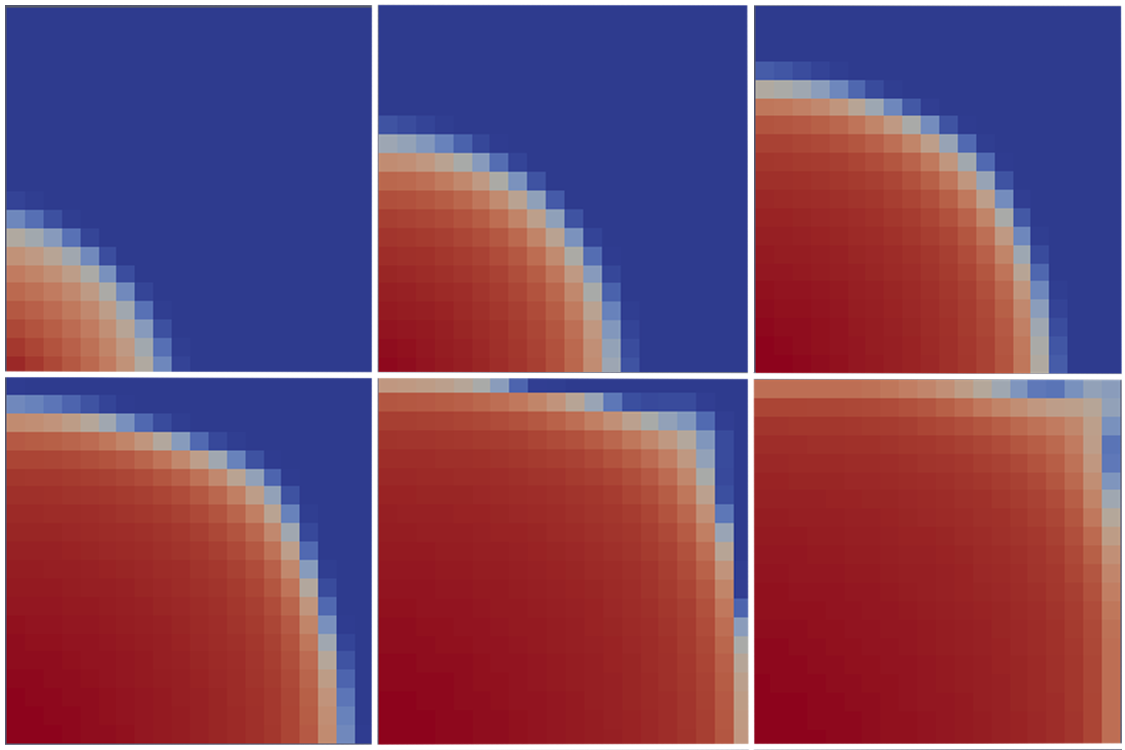
\includegraphics[width=0.6\textwidth]{figures/sat-hist-s-i-T-300-t-30-perm-10.png}};
\end{tikzpicture}
\caption{$S_w$ profile when solving the Q5 problem on a 20x20 grid with $t_{\text{end}} = \unit[300]{d}$ and $\Delta t = \unit[60]{d}$. The region has a homogeneous permeability of $\unit[10]{mD}$. Blue is oil, red is water.}
\label{fig:sat_hist_hom}
\end{figure}

%%%%%%%%%%%%  QUARTER FIVE SPOT %%%%%%%%%%
\subsection{Case A: Quarter Five Spot}
\label{section:caseA}
\todoinline{Error plot against reference solver for hom. Q5}
The \emph{quarter five spot}, abbreviated Q5, is a quadratic 2D domain with a source in one corner and a sink in the opposite corner along the diagonal. Here the domain has dimensions $\unit[120]{m}\times\unit[120]{m}\times\unit[10]{m}$. The fluid density is set to $\unitfrac[1000]{kg}{m^3}$, porosity $\unit[0.5]{}$ and the formation has homogeneous permeability $\unit[10]{mD}$. The simulation is run on a $20\times 20$ grid with a strong source in one corner cell and a sink in the diagonally opposite corner, both of magnitude $\unitfrac[180]{m^3}{s}$. The viscosity is varied through three cases; $\mu_w = \unit[1]{cP}$ and $\mu_o= \unit[1]{cP}$, $\mu_w = \unit[1]{cP}$ and $\mu_o= \unit[10]{cP}$, and $\mu_w = \unit[10]{cP}$ and $\mu_o= \unit[1]{cP}$. Figure \ref{fig:sat_hist_hom} shows an example of an advancing saturation profile from a simulation of the homogeneous Q5 problem. Because of the uniform permeability and the quadratic geometry the saturation profile is symmetric around the diagonal between the source and sink.

%%%%% 120 by 120 %%%%%%%
\subsubsection{120 m by 120 m comments}
The total iteration count spent when solving the Q5 problem is presented in Figures \ref{fig:caseA_iterations_t_5} and \ref{fig:caseA_iterations_t_5} for all root finders. We include the viscosity ratio because of the significant influence it has on the shape of $f_w$, as indicated by Figure \ref{fig:fractional_flow_wrt_viscosity_ratio}. The trend in the data is that Brent's method uses the highest number of iterations, while the trust region scheme needs significantly fewer iterations than all other methods. The data also indicates that the average iteration count is lower for larger $M$-values, and that the differences between the methods are smaller.

The total CPU running times are shown as a function of the time step $\Delta t$ for three different viscosity ratios $M$ in Figure \ref{fig:q5_homperm_10}. Again we include different $M$ values. With $M = 0.1$ all methods have similar performance up to around $\Delta t = \unit[20]{d}$, as shown in Figure \ref{fig:q5_cputime_perm_h_10_m_1_10_i_4}. At this point the regula falsi method, and a little later also the approximate trust region scheme, starts to spend more CPU time than the other methods. This trend is consistent over all subsequent time step sizes. We note that the other methods has equal performance for all time steps.
Next, Figure \ref{fig:q5_cputime_perm_h_10_m_1_1_i_4} shows the results for $M = 1$. Here all the root finders uses equal CPU time over the whole range of time steps.
Finally, $M = 10$ gives the results in Figure \ref{fig:q5_cputime_perm_h_10_m_10_1_i_4}. In this case the regula falsi is faster than all the other methods for $\Delta t \gtrapprox \unit[20]{d}$. Further we observe that the Ridders and Brent methods break of last at $\Delta t \approx \unit[20]{d}$, while the trust region scheme breaks of at $\Delta t \approx \unit[5]{d}$, and the approximate trust region scheme does the same at $\Delta t \approx \unit[10]{d}$.

\begin{figure}[!ht]
\centering
\tikzsetnextfilename{q5_hom_m-0_1}
\begin{subfigure}[b]{0.8\textwidth}
\begin{tikzpicture}
    \begin{semilogyaxis}[
            width=0.97\textwidth,
            height=0.26\textheight,
            xlabel={dt~[days]},
            ylabel={CPU time~[s]},
            grid=major,
            ]
        \addplot table[col sep=comma, trim cells=true,x=dt, y=cputime] {datafiles/q5-cputvsdt-s-r-T-300-m-1-10-dim-120-120-20-20-perm-h-10-i-180.data};
        \addplot table[col sep=comma, trim cells=true,x=dt, y=cputime] {datafiles/q5-cputvsdt-s-t-T-300-m-1-10-dim-120-120-20-20-perm-h-10-i-180.data};
        \addplot table[col sep=comma, trim cells=true,x=dt, y=cputime] {datafiles/q5-cputvsdt-s-a-T-300-m-1-10-dim-120-120-20-20-perm-h-10-i-180.data};
        \addplot table[col sep=comma, trim cells=true,x=dt, y=cputime] {datafiles/q5-cputvsdt-s-b-T-300-m-1-10-dim-120-120-20-20-perm-h-10-i-180.data};
        \addplot table[col sep=comma, trim cells=true,x=dt, y=cputime] {datafiles/q5-cputvsdt-s-i-T-300-m-1-10-dim-120-120-20-20-perm-h-10-i-180.data};
                \addplot table[col sep=comma, trim cells=true,x=dt, y=cputime] {datafiles/q5-cputvsdt-s-g-T-300-m-1-10-dim-120-120-20-20-perm-h-10-i-180.data};
        \legend{RF,TR,TR*,B,R,GN}
    \end{semilogyaxis}
\end{tikzpicture}%
\caption{$M =0.1$} \label{fig:q5_homperm_viscrat_0_1}
\end{subfigure}%
\vspace{0.3cm}
\centering
\tikzsetnextfilename{q5_hom_m-1_0}
\begin{subfigure}[b]{0.8\textwidth}
\begin{tikzpicture}
    \begin{semilogyaxis}[
            width=0.97\textwidth,
            height=0.26\textheight,
            xlabel={dt~[days]},
            ylabel={CPU time~[s]},
            grid=major,
            ]
         \addplot table[col sep=comma, trim cells=true,x=dt, y=cputime] {datafiles/q5-cputvsdt-s-r-T-300-m-1-1-dim-120-120-20-20-perm-h-10-i-180.data};
        \addplot table[col sep=comma, trim cells=true,x=dt, y=cputime] {datafiles/q5-cputvsdt-s-t-T-300-m-1-1-dim-120-120-20-20-perm-h-10-i-180.data};
        \addplot table[col sep=comma, trim cells=true,x=dt, y=cputime] {datafiles/q5-cputvsdt-s-a-T-300-m-1-1-dim-120-120-20-20-perm-h-10-i-180.data};
        \addplot table[col sep=comma, trim cells=true,x=dt, y=cputime] {datafiles/q5-cputvsdt-s-b-T-300-m-1-1-dim-120-120-20-20-perm-h-10-i-180.data};
        \addplot table[col sep=comma, trim cells=true,x=dt, y=cputime] {datafiles/q5-cputvsdt-s-i-T-300-m-1-1-dim-120-120-20-20-perm-h-10-i-180.data};
                \addplot table[col sep=comma, trim cells=true,x=dt, y=cputime] {datafiles/q5-cputvsdt-s-g-T-300-m-1-1-dim-120-120-20-20-perm-h-10-i-180.data};
        \legend{RF,TR,TR*,B,R,GN}
    \end{semilogyaxis}
\end{tikzpicture}%
\caption{$M =1$} \label{fig:q5_homperm_viscrat_1}
\end{subfigure}%
\vspace{0.3cm}
\centering
\tikzsetnextfilename{q5_hom_m-10_0}
\begin{subfigure}[b]{0.8\textwidth}
\begin{tikzpicture}
    \begin{semilogyaxis}[
            width=0.97\textwidth,
            height=0.26\textheight,
            xlabel={dt~[days]},
            ylabel={CPU time~[s]},
            grid=major,
            ]
         \addplot table[col sep=comma, trim cells=true,x=dt, y=cputime] {datafiles/q5-cputvsdt-s-r-T-300-m-10-1-dim-120-120-20-20-perm-h-10-i-180.data};
        \addplot table[col sep=comma, trim cells=true,x=dt, y=cputime] {datafiles/q5-cputvsdt-s-t-T-300-m-10-1-dim-120-120-20-20-perm-h-10-i-180.data};
        \addplot table[col sep=comma, trim cells=true,x=dt, y=cputime] {datafiles/q5-cputvsdt-s-a-T-300-m-10-1-dim-120-120-20-20-perm-h-10-i-180.data};
        \addplot table[col sep=comma, trim cells=true,x=dt, y=cputime] {datafiles/q5-cputvsdt-s-b-T-300-m-10-1-dim-120-120-20-20-perm-h-10-i-180.data};
        \addplot table[col sep=comma, trim cells=true,x=dt, y=cputime] {datafiles/q5-cputvsdt-s-i-T-300-m-10-1-dim-120-120-20-20-perm-h-10-i-180.data};
                \addplot table[col sep=comma, trim cells=true,x=dt, y=cputime] {datafiles/q5-cputvsdt-s-g-T-300-m-10-1-dim-120-120-20-20-perm-h-10-i-180.data};
        \legend{RF,TR,TR*,B,R,GN}
    \end{semilogyaxis}
\end{tikzpicture}%
\caption{$M =10$} \label{fig:q5_homperm_viscrat_10}
\end{subfigure}%
\caption{CPU time used to solve the Q5 problem, Section \ref{section:caseA}, for varying root finders, time steps and viscosity ratios.}
\label{fig:q5_homperm_10}
\end{figure}
\begin{figure}[!ht]
\tikzsetnextfilename{q5_iterations_perm_h_10_m_1_10_i_180_dt_1to30}
\begin{subfigure}[b]{0.49\textwidth} %%%%%%%%%%% M = 0.1 %%%%%%%%%%%%%%
\begin{tikzpicture}
    \pgfplotstablegetrowsof{datafiles/q5-iterations-s-r-T-300-m-1-10-dim-120-120-20-20-perm-h-10-i-180.data}
    \pgfmathsetmacro\yfin{\pgfmathresult}
    \pgfmathsetmacro\yini{5}
    \begin{semilogyaxis}[
            width=0.97\textwidth,
            height=0.26\textheight,
            ymin=9999,
            ymax=600000,
            xlabel={dt~[d]},
            ylabel={\#iterations},
            grid=both,
            skip coords between index={\yini}{\yfin}
            ]
        \addplot table[col sep=comma, trim cells=true,x=dt, y=iterations] {datafiles/q5-iterations-s-r-T-300-m-1-10-dim-120-120-20-20-perm-h-10-i-180.data};
        \addplot table[col sep=comma, trim cells=true,x=dt, y=iterations] {datafiles/q5-iterations-s-t-T-300-m-1-10-dim-120-120-20-20-perm-h-10-i-180.data};
        \addplot table[col sep=comma, trim cells=true,x=dt, y=iterations] {datafiles/q5-iterations-s-a-T-300-m-1-10-dim-120-120-20-20-perm-h-10-i-180.data};
        \addplot table[col sep=comma, trim cells=true,x=dt, y=iterations] {datafiles/q5-iterations-s-b-T-300-m-1-10-dim-120-120-20-20-perm-h-10-i-180.data};
        \addplot table[col sep=comma, trim cells=true,x=dt, y=iterations] {datafiles/q5-iterations-s-i-T-300-m-1-10-dim-120-120-20-20-perm-h-10-i-180.data};
        \legend{RF,TR,TR*,B,R}
    \end{semilogyaxis}
\end{tikzpicture}%
\caption{$M =0.1$} \label{fig:q5_iterations_perm_h_10_m_1_10_i_180_dt_1to30}
\end{subfigure}%
~
\tikzsetnextfilename{q5_iterations_perm_h_10_m_1_10_i_180_dt_40to150}
\begin{subfigure}[b]{0.49\textwidth}
\begin{tikzpicture}
    \pgfplotstablegetrowsof{datafiles/q5-iterations-s-r-T-300-m-1-10-dim-120-120-20-20-perm-h-10-i-180.data}
    \pgfmathsetmacro\yfin{5}
    \pgfmathsetmacro\yini{0}
    \begin{semilogyaxis}[
            width=0.97\textwidth,
            height=0.26\textheight,
            ymin=999,
            ymax=20000,
            xlabel={dt~[d]},
            ylabel={\#iterations},
            grid=both,
            skip coords between index={\yini}{\yfin}
            ]
        \addplot table[col sep=comma, trim cells=true,x=dt, y=iterations] {datafiles/q5-iterations-s-r-T-300-m-1-10-dim-120-120-20-20-perm-h-10-i-180.data};
        \addplot table[col sep=comma, trim cells=true,x=dt, y=iterations] {datafiles/q5-iterations-s-t-T-300-m-1-10-dim-120-120-20-20-perm-h-10-i-180.data};
        \addplot table[col sep=comma, trim cells=true,x=dt, y=iterations] {datafiles/q5-iterations-s-a-T-300-m-1-10-dim-120-120-20-20-perm-h-10-i-180.data};
        \addplot table[col sep=comma, trim cells=true,x=dt, y=iterations] {datafiles/q5-iterations-s-b-T-300-m-1-10-dim-120-120-20-20-perm-h-10-i-180.data};
        \addplot table[col sep=comma, trim cells=true,x=dt, y=iterations] {datafiles/q5-iterations-s-i-T-300-m-1-10-dim-120-120-20-20-perm-h-10-i-180.data};
        %\legend{RF,TR,TR*,B,R}
    \end{semilogyaxis}
\end{tikzpicture}%
\caption{$M =0.1$} \label{fig:q5_iterations_perm_h_10_m_1_10_i_180_dt_40to150}
\end{subfigure}%
\vspace{0.3cm} %%%%%%%%%%% M = 1 %%%%%%%%%%%%%%
\tikzsetnextfilename{q5_iterations_perm_h_10_m_1_1_i_180_dt_1to30}
\begin{subfigure}[b]{0.49\textwidth}
\begin{tikzpicture}
    \pgfplotstablegetrowsof{datafiles/q5-iterations-s-r-T-300-m-1-10-dim-120-120-20-20-perm-h-10-i-180.data}
    \pgfmathsetmacro\yfin{\pgfmathresult}
    \pgfmathsetmacro\yini{5}
    \begin{semilogyaxis}[
            width=0.97\textwidth,
            height=0.26\textheight,
            ymin=9999,
            ymax=600000,
            xlabel={dt~[d]},
            ylabel={\#iterations},
            grid=both,
            skip coords between index={\yini}{\yfin}
            ]
         \addplot table[col sep=comma, trim cells=true,x=dt, y=iterations] {datafiles/q5-iterations-s-r-T-300-m-1-1-dim-120-120-20-20-perm-h-10-i-180.data};
        \addplot table[col sep=comma, trim cells=true,x=dt, y=iterations] {datafiles/q5-iterations-s-t-T-300-m-1-1-dim-120-120-20-20-perm-h-10-i-180.data};
        \addplot table[col sep=comma, trim cells=true,x=dt, y=iterations] {datafiles/q5-iterations-s-a-T-300-m-1-1-dim-120-120-20-20-perm-h-10-i-180.data};
        \addplot table[col sep=comma, trim cells=true,x=dt, y=iterations] {datafiles/q5-iterations-s-b-T-300-m-1-1-dim-120-120-20-20-perm-h-10-i-180.data};
        \addplot table[col sep=comma, trim cells=true,x=dt, y=iterations] {datafiles/q5-iterations-s-i-T-300-m-1-1-dim-120-120-20-20-perm-h-10-i-180.data};
        \legend{RF,TR,TR*,B,R}
    \end{semilogyaxis}
\end{tikzpicture}%
\caption{$M =1$} \label{fig:q5_iterations_perm_h_10_m_1_1_i_180_dt_1to30}
\end{subfigure}%
~
\tikzsetnextfilename{q5_iterations_perm_h_10_m_1_1_i_180_dt_40to150}
\begin{subfigure}[b]{0.49\textwidth}
\begin{tikzpicture}
    \pgfplotstablegetrowsof{datafiles/q5-iterations-s-r-T-300-m-1-10-dim-120-120-20-20-perm-h-10-i-180.data}
    \pgfmathsetmacro\yfin{5}
    \pgfmathsetmacro\yini{0}
    \begin{semilogyaxis}[
            width=0.97\textwidth,
            height=0.26\textheight,
            ymin=999,
            ymax=20000,
            xlabel={dt~[d]},
            ylabel={\#iterations},
            grid=both,
            skip coords between index={\yini}{\yfin}
            ]
         \addplot table[col sep=comma, trim cells=true,x=dt, y=iterations] {datafiles/q5-iterations-s-r-T-300-m-1-1-dim-120-120-20-20-perm-h-10-i-180.data};
        \addplot table[col sep=comma, trim cells=true,x=dt, y=iterations] {datafiles/q5-iterations-s-t-T-300-m-1-1-dim-120-120-20-20-perm-h-10-i-180.data};
        \addplot table[col sep=comma, trim cells=true,x=dt, y=iterations] {datafiles/q5-iterations-s-a-T-300-m-1-1-dim-120-120-20-20-perm-h-10-i-180.data};
        \addplot table[col sep=comma, trim cells=true,x=dt, y=iterations] {datafiles/q5-iterations-s-b-T-300-m-1-1-dim-120-120-20-20-perm-h-10-i-180.data};
        \addplot table[col sep=comma, trim cells=true,x=dt, y=iterations] {datafiles/q5-iterations-s-i-T-300-m-1-1-dim-120-120-20-20-perm-h-10-i-180.data};
        %\legend{RF,TR,TR*,B,R}
    \end{semilogyaxis}
\end{tikzpicture}%
\caption{$M =1$} \label{fig:q5_iterations_perm_h_10_m_1_1_i_180_dt_40to150}
\end{subfigure}%
\vspace{0.3cm} %%%%%%%%%%% M = 10 %%%%%%%%%%%%%%
\tikzsetnextfilename{q5_iterations_perm_h_10_m_10_1_i_180_dt_1to30}
\begin{subfigure}[b]{0.49\textwidth}
\begin{tikzpicture}
    \pgfplotstablegetrowsof{datafiles/q5-iterations-s-r-T-300-m-1-10-dim-120-120-20-20-perm-h-10-i-180.data}
    \pgfmathsetmacro\yfin{\pgfmathresult}
    \pgfmathsetmacro\yini{5}
    \begin{semilogyaxis}[
            width=0.97\textwidth,
            height=0.26\textheight,
            ymin=8000,
            ymax=600000,
            xlabel={dt~[d]},
            ylabel={\#iterations},
            grid=both,
            skip coords between index={\yini}{\yfin}
            ]
         \addplot table[col sep=comma, trim cells=true,x=dt, y=iterations] {datafiles/q5-iterations-s-r-T-300-m-10-1-dim-120-120-20-20-perm-h-10-i-180.data};
        \addplot table[col sep=comma, trim cells=true,x=dt, y=iterations] {datafiles/q5-iterations-s-t-T-300-m-10-1-dim-120-120-20-20-perm-h-10-i-180.data};
        \addplot table[col sep=comma, trim cells=true,x=dt, y=iterations] {datafiles/q5-iterations-s-a-T-300-m-10-1-dim-120-120-20-20-perm-h-10-i-180.data};
        \addplot table[col sep=comma, trim cells=true,x=dt, y=iterations] {datafiles/q5-iterations-s-b-T-300-m-10-1-dim-120-120-20-20-perm-h-10-i-180.data};
        \addplot table[col sep=comma, trim cells=true,x=dt, y=iterations] {datafiles/q5-iterations-s-i-T-300-m-10-1-dim-120-120-20-20-perm-h-10-i-180.data};
        \legend{RF,TR,TR*,B,R}
    \end{semilogyaxis}
\end{tikzpicture}%
\caption{$M =10$} \label{fig:q5_iterations_perm_h_10_m_10_1_i_180_dt_1to30}
\end{subfigure}%
~
\tikzsetnextfilename{q5_iterations_perm_h_10_m_10_1_i_180_dt_40to150}
\begin{subfigure}[b]{0.49\textwidth}
\begin{tikzpicture}
    \pgfplotstablegetrowsof{datafiles/q5-iterations-s-r-T-300-m-1-10-dim-120-120-20-20-perm-h-10-i-180.data}
    \pgfmathsetmacro\yfin{5}
    \pgfmathsetmacro\yini{0}
    \begin{semilogyaxis}[
            width=0.97\textwidth,
            height=0.26\textheight,
            ymin=999,
            ymax=20000,
            xlabel={dt~[d]},
            ylabel={\#iterations},
            grid=both,
            skip coords between index={\yini}{\yfin}
            ]
         \addplot table[col sep=comma, trim cells=true,x=dt, y=iterations] {datafiles/q5-iterations-s-r-T-300-m-10-1-dim-120-120-20-20-perm-h-10-i-180.data};
        \addplot table[col sep=comma, trim cells=true,x=dt, y=iterations] {datafiles/q5-iterations-s-t-T-300-m-10-1-dim-120-120-20-20-perm-h-10-i-180.data};
        \addplot table[col sep=comma, trim cells=true,x=dt, y=iterations] {datafiles/q5-iterations-s-a-T-300-m-10-1-dim-120-120-20-20-perm-h-10-i-180.data};
        \addplot table[col sep=comma, trim cells=true,x=dt, y=iterations] {datafiles/q5-iterations-s-b-T-300-m-10-1-dim-120-120-20-20-perm-h-10-i-180.data};
        \addplot table[col sep=comma, trim cells=true,x=dt, y=iterations] {datafiles/q5-iterations-s-i-T-300-m-10-1-dim-120-120-20-20-perm-h-10-i-180.data};
        %\legend{RF,TR,TR*,B,R}
    \end{semilogyaxis}
\end{tikzpicture}%
\caption{$M =10$} \label{fig:q5_iterations_perm_h_10_m_10_1_i_180_dt_40to150}
\end{subfigure}%
\caption{\#iterations used to solve a modified Q5 problem, Section \ref{section:caseA}, for varying root finders, time steps and viscosity ratios. Note that $\unit[120]{m} \times \unit[120]{m}$ cells are used here.}
\label{fig:q5_iterations_perm_h_10_i_180}
\end{figure}%
%
%\begin{figure}[!ht]
%\centering
%\tikzsetnextfilename{q5_iterations_perm_h_10_m_1_10_i_180}
%\begin{subfigure}[b]{0.8\textwidth}
%\begin{tikzpicture}
%    \pgfplotstablegetrowsof{datafiles/q5-iterations-s-r-T-300-m-1-10-dim-120-120-20-20-perm-h-10-i-180.data}
%    \pgfmathsetmacro\yfin{\pgfmathresult - 4}
%    \pgfmathsetmacro\yini{0}
%    \begin{semilogyaxis}[
%            width=0.97\textwidth,
%            height=0.26\textheight,
%            ymin=1000,
%            ymax=1000000,
%            xlabel={dt~[d]},
%            ylabel={\#iterations},
%            grid=both,
%            ]
%        \addplot table[col sep=comma, trim cells=true,x=dt, y=iterations] {datafiles/q5-iterations-s-r-T-300-m-1-10-dim-120-120-20-20-perm-h-10-i-180.data};
%        \addplot table[col sep=comma, trim cells=true,x=dt, y=iterations] {datafiles/q5-iterations-s-t-T-300-m-1-10-dim-120-120-20-20-perm-h-10-i-180.data};
%        \addplot table[col sep=comma, trim cells=true,x=dt, y=iterations] {datafiles/q5-iterations-s-a-T-300-m-1-10-dim-120-120-20-20-perm-h-10-i-180.data};
%        \addplot table[col sep=comma, trim cells=true,x=dt, y=iterations] {datafiles/q5-iterations-s-b-T-300-m-1-10-dim-120-120-20-20-perm-h-10-i-180.data};
%        \addplot table[col sep=comma, trim cells=true,x=dt, y=iterations] {datafiles/q5-iterations-s-i-T-300-m-1-10-dim-120-120-20-20-perm-h-10-i-180.data};
%                %\addplot table[col sep=comma, trim cells=true,x=dt, y=iterations] {datafiles/q5-iterations-s-g-T-300-m-1-10-dim-120-120-20-20-perm-h-10-i-180.data};
%        \legend{RF,TR,TR*,B,R}
%    \end{semilogyaxis}
%\end{tikzpicture}%
%\caption{$M =0.1$} \label{fig:q5_iterations_perm_h_10_m_1_10_i_180}
%\end{subfigure}%
%\vspace{0.3cm}
%\centering
%\tikzsetnextfilename{q5_iterations_perm_h_10_m_1_1_i_180}
%\begin{subfigure}[b]{0.8\textwidth}
%\begin{tikzpicture}
%    \begin{semilogyaxis}[
%            width=0.97\textwidth,
%            height=0.26\textheight,
%            ymin=1000,
%            ymax=1000000,
%            xlabel={dt~[d]},
%            ylabel={\#iterations},
%            grid=both,
%            ]
%         \addplot table[col sep=comma, trim cells=true,x=dt, y=iterations] {datafiles/q5-iterations-s-r-T-300-m-1-1-dim-120-120-20-20-perm-h-10-i-180.data};
%        \addplot table[col sep=comma, trim cells=true,x=dt, y=iterations] {datafiles/q5-iterations-s-t-T-300-m-1-1-dim-120-120-20-20-perm-h-10-i-180.data};
%        \addplot table[col sep=comma, trim cells=true,x=dt, y=iterations] {datafiles/q5-iterations-s-a-T-300-m-1-1-dim-120-120-20-20-perm-h-10-i-180.data};
%        \addplot table[col sep=comma, trim cells=true,x=dt, y=iterations] {datafiles/q5-iterations-s-b-T-300-m-1-1-dim-120-120-20-20-perm-h-10-i-180.data};
%        \addplot table[col sep=comma, trim cells=true,x=dt, y=iterations] {datafiles/q5-iterations-s-i-T-300-m-1-1-dim-120-120-20-20-perm-h-10-i-180.data};
%                %\addplot table[col sep=comma, trim cells=true,x=dt, y=iterations] {datafiles/q5-iterations-s-g-T-300-m-1-1-dim-120-120-20-20-perm-h-10-i-180.data};
%        \legend{RF,TR,TR*,B,R}
%    \end{semilogyaxis}
%\end{tikzpicture}%
%\caption{$M =1$} \label{fig:q5_iterations_perm_h_10_m_1_1_i_180}
%\end{subfigure}%
%\vspace{0.3cm}
%\centering
%\tikzsetnextfilename{q5_iterations_perm_h_10_m_10_1_i_180}
%\begin{subfigure}[b]{0.8\textwidth}
%\begin{tikzpicture}
%    \begin{semilogyaxis}[
%            width=0.97\textwidth,
%            height=0.26\textheight,
%            ymin=1000,
%            ymax=1000000,
%            xlabel={dt~[d]},
%            ylabel={\#iterations},
%            grid=both,
%            ]
%         \addplot table[col sep=comma, trim cells=true,x=dt, y=iterations] {datafiles/q5-iterations-s-r-T-300-m-10-1-dim-120-120-20-20-perm-h-10-i-180.data};
%        \addplot table[col sep=comma, trim cells=true,x=dt, y=iterations] {datafiles/q5-iterations-s-t-T-300-m-10-1-dim-120-120-20-20-perm-h-10-i-180.data};
%        \addplot table[col sep=comma, trim cells=true,x=dt, y=iterations] {datafiles/q5-iterations-s-a-T-300-m-10-1-dim-120-120-20-20-perm-h-10-i-180.data};
%        \addplot table[col sep=comma, trim cells=true,x=dt, y=iterations] {datafiles/q5-iterations-s-b-T-300-m-10-1-dim-120-120-20-20-perm-h-10-i-180.data};
%        \addplot table[col sep=comma, trim cells=true,x=dt, y=iterations] {datafiles/q5-iterations-s-i-T-300-m-10-1-dim-120-120-20-20-perm-h-10-i-180.data};
%                %\addplot table[col sep=comma, trim cells=true,x=dt, y=iterations] {datafiles/q5-iterations-s-g-T-300-m-10-1-dim-120-120-20-20-perm-h-10-i-180.data};
%        \legend{RF,TR,TR*,B,R}
%    \end{semilogyaxis}
%\end{tikzpicture}%
%\caption{$M =10$} \label{fig:q5_iterations_perm_h_10_m_10_1_i_180}
%\end{subfigure}%
%\caption{\#iterations used to solve the Q5 problem, Section \ref{section:caseA}, for varying root finders, time steps and viscosity ratios.}
%\label{fig:q5_iterations_perm_h_10_i_180}
%\end{figure}

\subsubsubsection{Discussion}
A comparison of the iteration count and total CPU time results for test case A, shown in Figure \ref{fig:caseA_iterations_t_5} and \ref{fig:q5_cputime_perm_h_10_i_4}, respectively, highlights the differences in computational complexity for the different root finders. That is, even with the quite significant variation in total amount of iterations the CPU time is comparable for all root finders over the range of tested parameters. For instance, the trust region methods, which are essentially Newton methods, converge fast in terms of number of iterations due to the quadratic convergence of the Newton-Raphson scheme. But, since each iteration requires two function evaluations, one for the function itself and one for the derivative, the gains in iterations are balanced by a high overhead in each iteration. Similarly, the Brent method has ``only'' superlinear convergence and thus uses a very high number of iterations, but since it requires just one function evaluation per iteration the total CPU time spent is again normalized. Similar considerations can be used to explain the iteration count versus CPU time results for the other root finders.

\begin{itemize}
\item NB: The following observations are from simulation with $\Delta t = \unit[50]{d}$, 120 by 120 m!
\item $M = 0.1$: $\mu_{e_r} = 0.0814, \sigma_{e_r} = 0.0677$, $\mu_{S_r} = 0.3549, \sigma_{S_r} = 0.1832$
\item $M = 1$: $\mu_{e_r} = 0.1219, \sigma_{e_r} = 0.1242$, $\mu_{S_r} = 0.4815, \sigma_{S_r} = 0.3104$
\item $M = 10$: $\mu_{e_r} = 0.1474, \sigma_{e_r} = 0.2192$, $\mu_{S_r} = 0.5224, \sigma_{S_r} = 0.4210$
\item Large $M$ gives small $f_w$, i.e. lower flow of water out of cell. This gives higher water saturation on average.
\end{itemize}

Figure \ref{fig:q5_root_saturations_t_50} shows the distribution of the cell saturations $S_V^{n+1}$ for all time steps $\Delta t$ and three different viscosity ratios. The mean and standard deviation of the distributions, shown in Table \ref{table:q5_saturations_statisitcs_t_50}, indicates that the viscosity ratio $M$ has significant impact on the final saturation distribution in the domain. It seems that a large $M$ gives a larger average water saturation in the cells, while smaller $M$ gives smaller average saturation values. The trend in the shape of the distribution is even clearer, with larger values of $M$ pushing the distribution to the right and leaving a larger fraction of saturations near zero. These observations are readily explained by again noting that small $M$ gives values of the fractional water flow function $f_w$ closer to one, while larger $M$ keeps $f_w$ close to zero, as shown in Figure \ref{fig:fractional_flow_wrt_viscosity_ratio}. The $f_w$ measures the water flow, and scales the outgoing flux in the transport residual, Equation (\ref{eq:residual_two_phase_transport_simple}). Thus, large $f_w$ values gives a large flow of water out of the cell, while small gives a small flow. A large outflow of water will lead to smaller saturation values in the cell, and vice versa, which is exactly what we observe in Figure \ref{fig:q5_root_saturations_t_50}.

\begin{table}%
\caption{Standard deviation $\sigma$ and mean $\mu$ of the converged cell saturations $S^{n+1}$ in Figure \ref{fig:q5_root_saturations_t_50_i_180} and the initial guess error $e_{S_0} = \lvert S^{n+1} - S^n \rvert$. The Q5 problem, Section \ref{section:caseA}, was solved with $\Delta t = \unit[50]{d}$ and viscosity ratio $M$.}%
\label{table:q5_saturations_statisitcs_t_50_i_180}%
\centering%
\begin{tabular}{ ccc cc }%
\hline
$M$ & $\mu_{S}$ & $\sigma_{S}$ & $\mu_{e}$ & $\sigma_{e}$ \\
\hline
0.1 & 0.3549 & 0.1832 & 0.0814 & 0.0677 \\
1 & 0.4815 & 0.3104 & 0.1219 & 0.1242 \\
10 & 0.5224 & 0.4210 & 0.1474 & 0.2192 \\
\hline
\end{tabular}%
\end{table}%

\textbf{The results from the saturation statistics indicates that the initial guess errors are significant for large $M$, i.e. $f_w$ small. Small outflow gives large saturation values, i.e. large M gives large saturation values. A sharp front, since the flow enters the cell easily but leaves slowly. Causes a large percentage of zero cells. Small M gives more equal flow in and out of the cell, causing a smeared front and more uniform saturation values. NB: Does small M imply flux values of comparable size in and out of the cell?  How does this correlate with the discussion from the convergence tests?}

\tikzsetnextfilename{q5_root_saturations_i_180}
\begin{figure}[!ht]
\centering
\begin{tikzpicture}
    \begin{axis}[
            width=0.97\textwidth,
            height=0.26\textheight,
            xmin=0,
            xmax=2400,
            xlabel={},
            ylabel={S},
            grid=major,
            xticklabels={,,},
            legend pos=north west,
            ]
        \addplot table[mark=none,header=false,x expr=\coordindex+1,y index=0] {datafiles/q5-sr-T-300-t-50-m-1-10-dim-120-120-10-20-20-1-perm-h-10-i-180.data};
        \addplot table[mark=none,header=false,x expr=\coordindex+1,y index=0] {datafiles/q5-sr-T-300-t-50-m-1-1-dim-120-120-10-20-20-1-perm-h-10-i-180.data};
        \addplot table[mark=none,header=false,x expr=\coordindex+1,y index=0] {datafiles/q5-sr-T-300-t-50-m-10-1-dim-120-120-10-20-20-1-perm-h-10-i-180.data};
        
        \addplot [blue, mark = *, nodes near coords=$\mu_{S_r}$,every node near coord/.style={anchor=100}] coordinates{(1560,0.3549)};
        \addplot [red, mark = *, nodes near coords=$\mu_{S_r}$,every node near coord/.style={anchor=120}] coordinates{(1400,0.4815)};
        \addplot [brown, mark = *, nodes near coords=$\mu_{S_r}$,every node near coord/.style={anchor=310}] coordinates{(1420,0.5224)};
        \legend{M=0.1,M=1,M=10}
    \end{axis}
\end{tikzpicture}%
\caption{Sorted cell saturations, 2400 in total, from all time steps for the solution of the Q5 problem in Section \ref{section:caseA} with $\Delta t = \unit[50]{d}$. Values for viscosity ratios $M=0.1$, $M=1$, and $M=10$ are reported with corresponding mean values $\mu_{S_r}$ at $0.3549$, $0.4815$, and $0.5224$, respectively.}
\label{fig:q5_root_saturations_t_50_i_180}
\end{figure}%
\tikzsetnextfilename{q5_initial_guess_errors_i_180}
\begin{figure}[!ht]
\centering
\begin{tikzpicture}
    \begin{axis}[
            width=0.97\textwidth,
            height=0.26\textheight,
            xmin=0,
            xmax=2400,
            xlabel={},
            ylabel={error},
            grid=both,
            xticklabels={,,},
            legend pos=north west,
            ]
        \addplot table[mark=none,header=false,x expr=\coordindex+1,y index=0] {datafiles/q5-s0error-T-300-t-50-m-1-10-dim-120-120-10-20-20-1-perm-h-10-i-180.data};
        \addplot table[mark=none,header=false,x expr=\coordindex+1,y index=0] {datafiles/q5-s0error-T-300-t-50-m-1-1-dim-120-120-10-20-20-1-perm-h-10-i-180.data};
        \addplot table[mark=none,header=false,x expr=\coordindex+1,y index=0] {datafiles/q5-s0error-T-300-t-50-m-10-1-dim-120-120-10-20-20-1-perm-h-10-i-180.data};
        \legend{M=0.1,M=1,M=10}
    \end{axis}
\end{tikzpicture}%
\caption{The initial root guess error $\lvert S_r - S^{n} \rvert,~S_r\colon R(S_r) = 0$ for each single cell problem, 2400 in total, for all time steps for the solution of the Q5 problem in Section \ref{section:caseA} with $\Delta t = \unit[50]{d}$. Values for viscosity ratios $M=0.1$, $M=1$, and $M=10$ are reported. Note that $\unit[120]{m} \times \unit[120]{m}$ cells are used here.}
\label{fig:q5_initial_guess_errors_t_50_i_180}
\end{figure}%

\clearpage
%%%%% 10 by 10 %%%%%%%
\subsubsection{10 m by 10 m comments}
The total number of iterations spent by each root finder when solving the Q5 problem is shown as a function of $\Delta t$ and the viscosity ratio $M$ in Figure \ref{fig:q5_iterations_perm_h_10_i_4}. The Brent methods spends the most iterations, while the regula falsi is a close second. Ridders method needs more iterations than the two trust region schemes. For $\Delta t \lessapprox 60$ the precise trust region scheme is the most efficient with the approximate trust region scheme a close second, while $\Delta t \gtrapprox 60$ favours the approximate trust region scheme. Qualitatively these observations are consistent for all tested viscosity ratios. Note however that the quantitative difference between the number of iterations spent by the various root finders is influenced by $M$. The qualitative difference between the methods are about as expected based on their theoretical convergence rates. The trust region schemes benefit from the quadratic local convergence of the underlying Newton scheme, while the other methods with only superlinear convergence need more iterations to obtain the desired precision. The advantage of the trust region schemes over the other methods seem quite significant.

\begin{figure}[!ht]
\tikzsetnextfilename{q5_iterations_perm_h_10_m_1_10_i_4_dt_1to30}
\begin{subfigure}[b]{0.49\textwidth} %%%%%%%%%%% M = 0.1 %%%%%%%%%%%%%%
\begin{tikzpicture}
    \pgfplotstablegetrowsof{datafiles/q5-iterations-s-r-T-300-m-1-10-dim-10-10-20-20-perm-h-10-i-4.data}
    \pgfmathsetmacro\yfin{\pgfmathresult}
    \pgfmathsetmacro\yini{5}
    \begin{semilogyaxis}[
            width=0.97\textwidth,
            height=0.26\textheight,
            ymin=10000,
            ymax=600000,
            xlabel={dt~[days]},
            ylabel={\#iterations},
            grid=major,
            skip coords between index={\yini}{\yfin}
            ]
        \addplot table[col sep=comma, trim cells=true,x=dt, y=iterations] {datafiles/q5-iterations-s-r-T-300-m-1-10-dim-10-10-20-20-perm-h-10-i-4.data};
        \addplot table[col sep=comma, trim cells=true,x=dt, y=iterations] {datafiles/q5-iterations-s-t-T-300-m-1-10-dim-10-10-20-20-perm-h-10-i-4.data};
        \addplot table[col sep=comma, trim cells=true,x=dt, y=iterations] {datafiles/q5-iterations-s-a-T-300-m-1-10-dim-10-10-20-20-perm-h-10-i-4.data};
        \addplot table[col sep=comma, trim cells=true,x=dt, y=iterations] {datafiles/q5-iterations-s-b-T-300-m-1-10-dim-10-10-20-20-perm-h-10-i-4.data};
        \addplot table[col sep=comma, trim cells=true,x=dt, y=iterations] {datafiles/q5-iterations-s-i-T-300-m-1-10-dim-10-10-20-20-perm-h-10-i-4.data};
        \legend{RF,TR,TR*,B,R}
    \end{semilogyaxis}
\end{tikzpicture}%
\caption{$M =0.1$} \label{fig:q5_iterations_perm_h_10_m_1_10_i_4_dt_1to30}
\end{subfigure}%
~
\tikzsetnextfilename{q5_iterations_perm_h_10_m_1_10_i_4_dt_40to150}
\begin{subfigure}[b]{0.49\textwidth}
\begin{tikzpicture}
    \pgfplotstablegetrowsof{datafiles/q5-iterations-s-r-T-300-m-1-10-dim-10-10-20-20-perm-h-10-i-4.data}
    \pgfmathsetmacro\yfin{5}
    \pgfmathsetmacro\yini{0}
    \begin{semilogyaxis}[
            width=0.97\textwidth,
            height=0.26\textheight,
            ymin=1000,
            ymax=20000,
            xlabel={dt~[days]},
            ylabel={\#iterations},
            grid=major,
            skip coords between index={\yini}{\yfin}
            ]
        \addplot table[col sep=comma, trim cells=true,x=dt, y=iterations] {datafiles/q5-iterations-s-r-T-300-m-1-10-dim-10-10-20-20-perm-h-10-i-4.data};
        \addplot table[col sep=comma, trim cells=true,x=dt, y=iterations] {datafiles/q5-iterations-s-t-T-300-m-1-10-dim-10-10-20-20-perm-h-10-i-4.data};
        \addplot table[col sep=comma, trim cells=true,x=dt, y=iterations] {datafiles/q5-iterations-s-a-T-300-m-1-10-dim-10-10-20-20-perm-h-10-i-4.data};
        \addplot table[col sep=comma, trim cells=true,x=dt, y=iterations] {datafiles/q5-iterations-s-b-T-300-m-1-10-dim-10-10-20-20-perm-h-10-i-4.data};
        \addplot table[col sep=comma, trim cells=true,x=dt, y=iterations] {datafiles/q5-iterations-s-i-T-300-m-1-10-dim-10-10-20-20-perm-h-10-i-4.data};
        %\legend{RF,TR,TR*,B,R}
    \end{semilogyaxis}
\end{tikzpicture}%
\caption{$M =0.1$} \label{fig:q5_iterations_perm_h_10_m_1_10_i_4_dt_40to150}
\end{subfigure}%
\vspace{0.3cm} %%%%%%%%%%% M = 1 %%%%%%%%%%%%%%
\tikzsetnextfilename{q5_iterations_perm_h_10_m_1_1_i_4_dt_1to30}
\begin{subfigure}[b]{0.49\textwidth}
\begin{tikzpicture}
    \pgfplotstablegetrowsof{datafiles/q5-iterations-s-r-T-300-m-1-10-dim-10-10-20-20-perm-h-10-i-4.data}
    \pgfmathsetmacro\yfin{\pgfmathresult}
    \pgfmathsetmacro\yini{5}
    \begin{semilogyaxis}[
            width=0.97\textwidth,
            height=0.26\textheight,
            ymin=10000,
            ymax=600000,
            xlabel={dt~[days]},
            ylabel={\#iterations},
            grid=major,
            skip coords between index={\yini}{\yfin}
            ]
         \addplot table[col sep=comma, trim cells=true,x=dt, y=iterations] {datafiles/q5-iterations-s-r-T-300-m-1-1-dim-10-10-20-20-perm-h-10-i-4.data};
        \addplot table[col sep=comma, trim cells=true,x=dt, y=iterations] {datafiles/q5-iterations-s-t-T-300-m-1-1-dim-10-10-20-20-perm-h-10-i-4.data};
        \addplot table[col sep=comma, trim cells=true,x=dt, y=iterations] {datafiles/q5-iterations-s-a-T-300-m-1-1-dim-10-10-20-20-perm-h-10-i-4.data};
        \addplot table[col sep=comma, trim cells=true,x=dt, y=iterations] {datafiles/q5-iterations-s-b-T-300-m-1-1-dim-10-10-20-20-perm-h-10-i-4.data};
        \addplot table[col sep=comma, trim cells=true,x=dt, y=iterations] {datafiles/q5-iterations-s-i-T-300-m-1-1-dim-10-10-20-20-perm-h-10-i-4.data};
        \legend{RF,TR,TR*,B,R}
    \end{semilogyaxis}
\end{tikzpicture}%
\caption{$M =1$} \label{fig:q5_iterations_perm_h_10_m_1_1_i_4_dt_1to30}
\end{subfigure}%
~
\tikzsetnextfilename{q5_iterations_perm_h_10_m_1_1_i_4_dt_40to150}
\begin{subfigure}[b]{0.49\textwidth}
\begin{tikzpicture}
    \pgfplotstablegetrowsof{datafiles/q5-iterations-s-r-T-300-m-1-10-dim-10-10-20-20-perm-h-10-i-4.data}
    \pgfmathsetmacro\yfin{5}
    \pgfmathsetmacro\yini{0}
    \begin{semilogyaxis}[
            width=0.97\textwidth,
            height=0.26\textheight,
            ymin=1000,
            ymax=20000,
            xlabel={dt~[days]},
            ylabel={\#iterations},
            grid=major,
            skip coords between index={\yini}{\yfin}
            ]
         \addplot table[col sep=comma, trim cells=true,x=dt, y=iterations] {datafiles/q5-iterations-s-r-T-300-m-1-1-dim-10-10-20-20-perm-h-10-i-4.data};
        \addplot table[col sep=comma, trim cells=true,x=dt, y=iterations] {datafiles/q5-iterations-s-t-T-300-m-1-1-dim-10-10-20-20-perm-h-10-i-4.data};
        \addplot table[col sep=comma, trim cells=true,x=dt, y=iterations] {datafiles/q5-iterations-s-a-T-300-m-1-1-dim-10-10-20-20-perm-h-10-i-4.data};
        \addplot table[col sep=comma, trim cells=true,x=dt, y=iterations] {datafiles/q5-iterations-s-b-T-300-m-1-1-dim-10-10-20-20-perm-h-10-i-4.data};
        \addplot table[col sep=comma, trim cells=true,x=dt, y=iterations] {datafiles/q5-iterations-s-i-T-300-m-1-1-dim-10-10-20-20-perm-h-10-i-4.data};
        %\legend{RF,TR,TR*,B,R}
    \end{semilogyaxis}
\end{tikzpicture}%
\caption{$M =1$} \label{fig:q5_iterations_perm_h_10_m_1_1_i_4_dt_40to150}
\end{subfigure}%
\vspace{0.3cm} %%%%%%%%%%% M = 10 %%%%%%%%%%%%%%
\tikzsetnextfilename{q5_iterations_perm_h_10_m_10_1_i_4_dt_1to30}
\begin{subfigure}[b]{0.49\textwidth}
\begin{tikzpicture}
    \pgfplotstablegetrowsof{datafiles/q5-iterations-s-r-T-300-m-1-10-dim-10-10-20-20-perm-h-10-i-4.data}
    \pgfmathsetmacro\yfin{\pgfmathresult}
    \pgfmathsetmacro\yini{5}
    \begin{semilogyaxis}[
            width=0.97\textwidth,
            height=0.26\textheight,
            ymin=8000,
            ymax=600000,
            xlabel={dt~[days]},
            ylabel={\#iterations},
            grid=major,
            skip coords between index={\yini}{\yfin}
            ]
         \addplot table[col sep=comma, trim cells=true,x=dt, y=iterations] {datafiles/q5-iterations-s-r-T-300-m-10-1-dim-10-10-20-20-perm-h-10-i-4.data};
        \addplot table[col sep=comma, trim cells=true,x=dt, y=iterations] {datafiles/q5-iterations-s-t-T-300-m-10-1-dim-10-10-20-20-perm-h-10-i-4.data};
        \addplot table[col sep=comma, trim cells=true,x=dt, y=iterations] {datafiles/q5-iterations-s-a-T-300-m-10-1-dim-10-10-20-20-perm-h-10-i-4.data};
        \addplot table[col sep=comma, trim cells=true,x=dt, y=iterations] {datafiles/q5-iterations-s-b-T-300-m-10-1-dim-10-10-20-20-perm-h-10-i-4.data};
        \addplot table[col sep=comma, trim cells=true,x=dt, y=iterations] {datafiles/q5-iterations-s-i-T-300-m-10-1-dim-10-10-20-20-perm-h-10-i-4.data};
        \legend{RF,TR,TR*,B,R}
    \end{semilogyaxis}
\end{tikzpicture}%
\caption{$M =10$} \label{fig:q5_iterations_perm_h_10_m_10_1_i_4_dt_1to30}
\end{subfigure}%
~
\tikzsetnextfilename{q5_iterations_perm_h_10_m_10_1_i_4_dt_40to150}
\begin{subfigure}[b]{0.49\textwidth}
\begin{tikzpicture}
    \pgfplotstablegetrowsof{datafiles/q5-iterations-s-r-T-300-m-1-10-dim-10-10-20-20-perm-h-10-i-4.data}
    \pgfmathsetmacro\yfin{5}
    \pgfmathsetmacro\yini{0}
    \begin{semilogyaxis}[
            width=0.97\textwidth,
            height=0.26\textheight,
            ymin=1000,
            ymax=20000,
            xlabel={dt~[days]},
            ylabel={\#iterations},
            grid=major,
            skip coords between index={\yini}{\yfin}
            ]
         \addplot table[col sep=comma, trim cells=true,x=dt, y=iterations] {datafiles/q5-iterations-s-r-T-300-m-10-1-dim-10-10-20-20-perm-h-10-i-4.data};
        \addplot table[col sep=comma, trim cells=true,x=dt, y=iterations] {datafiles/q5-iterations-s-t-T-300-m-10-1-dim-10-10-20-20-perm-h-10-i-4.data};
        \addplot table[col sep=comma, trim cells=true,x=dt, y=iterations] {datafiles/q5-iterations-s-a-T-300-m-10-1-dim-10-10-20-20-perm-h-10-i-4.data};
        \addplot table[col sep=comma, trim cells=true,x=dt, y=iterations] {datafiles/q5-iterations-s-b-T-300-m-10-1-dim-10-10-20-20-perm-h-10-i-4.data};
        \addplot table[col sep=comma, trim cells=true,x=dt, y=iterations] {datafiles/q5-iterations-s-i-T-300-m-10-1-dim-10-10-20-20-perm-h-10-i-4.data};
        %\legend{RF,TR,TR*,B,R}
    \end{semilogyaxis}
\end{tikzpicture}%
\caption{$M =10$} \label{fig:q5_iterations_perm_h_10_m_10_1_i_4_dt_40to150}
\end{subfigure}%
\caption{\#iterations used to solve the Q5 problem, Section \ref{section:caseA}, for varying root finders, time steps and viscosity ratios.}
\label{fig:q5_iterations_perm_h_10_i_4}
\end{figure}%
%
%\begin{figure}[!ht]
%\centering
%\tikzsetnextfilename{q5_iterations_perm_h_10_m_1_10_i_4}
%\begin{subfigure}[b]{0.8\textwidth}
%\begin{tikzpicture}
%    \pgfplotstablegetrowsof{datafiles/q5-iterations-s-r-T-300-m-1-10-dim-10-10-20-20-perm-h-10-i-4.data}
%    \pgfmathsetmacro\yfin{\pgfmathresult - 4}
%    \pgfmathsetmacro\yini{0}
%    \begin{semilogyaxis}[
%            width=0.97\textwidth,
%            height=0.26\textheight,
%            ymin=1000,
%            ymax=1000000,
%            xlabel={dt~[days]},
%            ylabel={\#iterations},
%            grid=major,
%            ]
%        \addplot table[col sep=comma, trim cells=true,x=dt, y=iterations] {datafiles/q5-iterations-s-r-T-300-m-1-10-dim-10-10-20-20-perm-h-10-i-4.data};
%        \addplot table[col sep=comma, trim cells=true,x=dt, y=iterations] {datafiles/q5-iterations-s-t-T-300-m-1-10-dim-10-10-20-20-perm-h-10-i-4.data};
%        \addplot table[col sep=comma, trim cells=true,x=dt, y=iterations] {datafiles/q5-iterations-s-a-T-300-m-1-10-dim-10-10-20-20-perm-h-10-i-4.data};
%        \addplot table[col sep=comma, trim cells=true,x=dt, y=iterations] {datafiles/q5-iterations-s-b-T-300-m-1-10-dim-10-10-20-20-perm-h-10-i-4.data};
%        \addplot table[col sep=comma, trim cells=true,x=dt, y=iterations] {datafiles/q5-iterations-s-i-T-300-m-1-10-dim-10-10-20-20-perm-h-10-i-4.data};
%                %\addplot table[col sep=comma, trim cells=true,x=dt, y=iterations] {datafiles/q5-iterations-s-g-T-300-m-1-10-dim-10-10-20-20-perm-h-10-i-4.data};
%        \legend{RF,TR,TR*,B,R}
%    \end{semilogyaxis}
%\end{tikzpicture}%
%\caption{$M =0.1$} \label{fig:q5_iterations_perm_h_10_m_1_10_i_4}
%\end{subfigure}%
%\vspace{0.3cm}
%\centering
%\tikzsetnextfilename{q5_iterations_perm_h_10_m_1_1_i_4}
%\begin{subfigure}[b]{0.8\textwidth}
%\begin{tikzpicture}
%    \begin{semilogyaxis}[
%            width=0.97\textwidth,
%            height=0.26\textheight,
%            ymin=1000,
%            ymax=1000000,
%            xlabel={dt~[days]},
%            ylabel={\#iterations},
%            grid=major,
%            ]
%         \addplot table[col sep=comma, trim cells=true,x=dt, y=iterations] {datafiles/q5-iterations-s-r-T-300-m-1-1-dim-10-10-20-20-perm-h-10-i-4.data};
%        \addplot table[col sep=comma, trim cells=true,x=dt, y=iterations] {datafiles/q5-iterations-s-t-T-300-m-1-1-dim-10-10-20-20-perm-h-10-i-4.data};
%        \addplot table[col sep=comma, trim cells=true,x=dt, y=iterations] {datafiles/q5-iterations-s-a-T-300-m-1-1-dim-10-10-20-20-perm-h-10-i-4.data};
%        \addplot table[col sep=comma, trim cells=true,x=dt, y=iterations] {datafiles/q5-iterations-s-b-T-300-m-1-1-dim-10-10-20-20-perm-h-10-i-4.data};
%        \addplot table[col sep=comma, trim cells=true,x=dt, y=iterations] {datafiles/q5-iterations-s-i-T-300-m-1-1-dim-10-10-20-20-perm-h-10-i-4.data};
%                %\addplot table[col sep=comma, trim cells=true,x=dt, y=iterations] {datafiles/q5-iterations-s-g-T-300-m-1-1-dim-10-10-20-20-perm-h-10-i-4.data};
%        \legend{RF,TR,TR*,B,R}
%    \end{semilogyaxis}
%\end{tikzpicture}%
%\caption{$M =1$} \label{fig:q5_iterations_perm_h_10_m_1_1_i_4}
%\end{subfigure}%
%\vspace{0.3cm}
%\centering
%\tikzsetnextfilename{q5_iterations_perm_h_10_m_10_1_i_4}
%\begin{subfigure}[b]{0.8\textwidth}
%\begin{tikzpicture}
%    \begin{semilogyaxis}[
%            width=0.97\textwidth,
%            height=0.26\textheight,
%            ymin=1000,
%            ymax=1000000,
%            xlabel={dt~[days]},
%            ylabel={\#iterations},
%            grid=major,
%            ]
%         \addplot table[col sep=comma, trim cells=true,x=dt, y=iterations] {datafiles/q5-iterations-s-r-T-300-m-10-1-dim-10-10-20-20-perm-h-10-i-4.data};
%        \addplot table[col sep=comma, trim cells=true,x=dt, y=iterations] {datafiles/q5-iterations-s-t-T-300-m-10-1-dim-10-10-20-20-perm-h-10-i-4.data};
%        \addplot table[col sep=comma, trim cells=true,x=dt, y=iterations] {datafiles/q5-iterations-s-a-T-300-m-10-1-dim-10-10-20-20-perm-h-10-i-4.data};
%        \addplot table[col sep=comma, trim cells=true,x=dt, y=iterations] {datafiles/q5-iterations-s-b-T-300-m-10-1-dim-10-10-20-20-perm-h-10-i-4.data};
%        \addplot table[col sep=comma, trim cells=true,x=dt, y=iterations] {datafiles/q5-iterations-s-i-T-300-m-10-1-dim-10-10-20-20-perm-h-10-i-4.data};
%                %\addplot table[col sep=comma, trim cells=true,x=dt, y=iterations] {datafiles/q5-iterations-s-g-T-300-m-10-1-dim-10-10-20-20-perm-h-10-i-4.data};
%        \legend{RF,TR,TR*,B,R}
%    \end{semilogyaxis}
%\end{tikzpicture}%
%\caption{$M =10$} \label{fig:q5_iterations_perm_h_10_m_10_1_i_4}
%\end{subfigure}%
%\caption{\#iterations used to solve the Q5 problem, Section \ref{section:caseA}, for varying root finders, time steps and viscosity ratios.}
%\label{fig:q5_iterations_perm_h_10_i_4}
%\end{figure}

The total CPU time spent when solving the Q5 problem is shown in Figure \ref{fig:q5_cputime_perm_h_10_i_4} for all root finders and different viscosity ratios. Starting with Figure \ref{fig:q5_cputime_perm_h_10_m_1_10_i_4} for $M = 0.1$ we see that the CPU times for all methods are practically indistinguishable up to $\Delta t \approx \unit[20]{d}$. At this point the precise trust region method becomes faster than the rest. This holds until $\Delta t \approx \unit[50]{d}$ where the regula falsi method also lowers its CPU time. Finally, the Brent method speeds up somewhere between $\Delta t = \unit[50]{d}$ and $\unit[50]{d}$. The Ridders method and the approximate trust region method have similar, and the lowest, performance for all time steps. The exception is the very last time step where the approximate trust region scheme jumps to the level of the fastest algorithms.

The timing results with $M = 1$ are shown in Figure \ref{fig:q5_cputime_perm_h_10_m_1_1_i_4}. The results in this case are less clear cut than with $M = 0.1$, with run times jumping up and down between time steps. We note a few trends though; First, the Ridders and approximate trust region methods have fairly consistent low timing results. Second, the regula falsi and precise trust region schemes perform worse than the two aforementioned methods for the mid range of time step values, between $\Delta t \approx \unit[20]{d}$ and $\Delta t \approx \unit[100]{d}$. After that they have good performance.

Finally, Figure \ref{fig:q5_cputime_perm_h_10_m_10_1_i_4} shows the results with viscosity ratio $M = 10$. Here the precise trust region method is consistently the most efficient method after all other methods break away between $\Delta t = \unit[20]{d}$ and $\unit[20]{d}$. The other methods have similar performance for the rest of the tested time steps.

A general observation is that all methods seems to have similar performance for the smallest time steps, up until around $\Delta t \approx \unit[20]{d}$.

\begin{itemize}
\item General impression from watching $M=0.1$ residuals: Root often close to inflection point.
\item -> Maybe check number of inflection point crossings?
\item $M=0.1$: Last time step has lots of relatively linear residuals
\item -> Perhaps trust region is comparably slow on linear residuals?
\end{itemize}

\begin{figure}[!ht]
\centering
\tikzsetnextfilename{q5_cputime_perm_h_10_m_1_10_i_4}
\begin{subfigure}[b]{0.8\textwidth}
\begin{tikzpicture}
    \begin{semilogyaxis}[
            width=0.97\textwidth,
            height=0.26\textheight,
            xlabel={dt~[d]},
            ylabel={CPU time~[s]},
            grid=both,
            ]
        \addplot table[col sep=comma, trim cells=true,x=dt, y=cputime] {datafiles/q5-cputvsdt-s-r-T-300-m-1-10-dim-10-10-20-20-perm-h-10-i-4.data};
        \addplot table[col sep=comma, trim cells=true,x=dt, y=cputime] {datafiles/q5-cputvsdt-s-t-T-300-m-1-10-dim-10-10-20-20-perm-h-10-i-4.data};
        \addplot table[col sep=comma, trim cells=true,x=dt, y=cputime] {datafiles/q5-cputvsdt-s-a-T-300-m-1-10-dim-10-10-20-20-perm-h-10-i-4.data};
        \addplot table[col sep=comma, trim cells=true,x=dt, y=cputime] {datafiles/q5-cputvsdt-s-b-T-300-m-1-10-dim-10-10-20-20-perm-h-10-i-4.data};
        \addplot table[col sep=comma, trim cells=true,x=dt, y=cputime] {datafiles/q5-cputvsdt-s-i-T-300-m-1-10-dim-10-10-20-20-perm-h-10-i-4.data};
                %\addplot table[col sep=comma, trim cells=true,x=dt, y=cputime] {datafiles/q5-cputvsdt-s-g-T-300-m-1-10-dim-10-10-20-20-perm-h-10-i-4.data};
        \legend{RF,TR,TR*,B,R}
    \end{semilogyaxis}
\end{tikzpicture}%
\caption{$M =0.1$} \label{fig:q5_cputime_perm_h_10_m_1_10_i_4}
\end{subfigure}%
\vspace{0.3cm}
\centering
\tikzsetnextfilename{q5_cputime_perm_h_10_m_1_1_i_4}
\begin{subfigure}[b]{0.8\textwidth}
\begin{tikzpicture}
    \begin{semilogyaxis}[
            width=0.97\textwidth,
            height=0.26\textheight,
            xlabel={dt~[d]},
            ylabel={CPU time~[s]},
            grid=both,
            ]
         \addplot table[col sep=comma, trim cells=true,x=dt, y=cputime] {datafiles/q5-cputvsdt-s-r-T-300-m-1-1-dim-10-10-20-20-perm-h-10-i-4.data};
        \addplot table[col sep=comma, trim cells=true,x=dt, y=cputime] {datafiles/q5-cputvsdt-s-t-T-300-m-1-1-dim-10-10-20-20-perm-h-10-i-4.data};
        \addplot table[col sep=comma, trim cells=true,x=dt, y=cputime] {datafiles/q5-cputvsdt-s-a-T-300-m-1-1-dim-10-10-20-20-perm-h-10-i-4.data};
        \addplot table[col sep=comma, trim cells=true,x=dt, y=cputime] {datafiles/q5-cputvsdt-s-b-T-300-m-1-1-dim-10-10-20-20-perm-h-10-i-4.data};
        \addplot table[col sep=comma, trim cells=true,x=dt, y=cputime] {datafiles/q5-cputvsdt-s-i-T-300-m-1-1-dim-10-10-20-20-perm-h-10-i-4.data};
                %\addplot table[col sep=comma, trim cells=true,x=dt, y=cputime] {datafiles/q5-cputvsdt-s-g-T-300-m-1-1-dim-10-10-20-20-perm-h-10-i-4.data};
        \legend{RF,TR,TR*,B,R}
    \end{semilogyaxis}
\end{tikzpicture}%
\caption{$M =1$} \label{fig:q5_cputime_perm_h_10_m_1_1_i_4}
\end{subfigure}%
\vspace{0.3cm}
\centering
\tikzsetnextfilename{q5_cputime_perm_h_10_m_10_1_i_4}
\begin{subfigure}[b]{0.8\textwidth}
\begin{tikzpicture}
    \begin{semilogyaxis}[
            width=0.97\textwidth,
            height=0.26\textheight,
            xlabel={dt~[d]},
            ylabel={CPU time~[s]},
            grid=both,
            ]
         \addplot table[col sep=comma, trim cells=true,x=dt, y=cputime] {datafiles/q5-cputvsdt-s-r-T-300-m-10-1-dim-10-10-20-20-perm-h-10-i-4.data};
        \addplot table[col sep=comma, trim cells=true,x=dt, y=cputime] {datafiles/q5-cputvsdt-s-t-T-300-m-10-1-dim-10-10-20-20-perm-h-10-i-4.data};
        \addplot table[col sep=comma, trim cells=true,x=dt, y=cputime] {datafiles/q5-cputvsdt-s-a-T-300-m-10-1-dim-10-10-20-20-perm-h-10-i-4.data};
        \addplot table[col sep=comma, trim cells=true,x=dt, y=cputime] {datafiles/q5-cputvsdt-s-b-T-300-m-10-1-dim-10-10-20-20-perm-h-10-i-4.data};
        \addplot table[col sep=comma, trim cells=true,x=dt, y=cputime] {datafiles/q5-cputvsdt-s-i-T-300-m-10-1-dim-10-10-20-20-perm-h-10-i-4.data};
                %\addplot table[col sep=comma, trim cells=true,x=dt, y=cputime] {datafiles/q5-cputvsdt-s-g-T-300-m-10-1-dim-10-10-20-20-perm-h-10-i-4.data};
        \legend{RF,TR,TR*,B,R}
    \end{semilogyaxis}
\end{tikzpicture}%
\caption{$M =10$} \label{fig:q5_cputime_perm_h_10_m_10_1_i_4}
\end{subfigure}%
\caption{CPU time used to solve the Q5 problem, Section \ref{section:caseA}, for varying root finders, time steps and viscosity ratios.}
\label{fig:q5_cputime_perm_h_10_i_4}
\end{figure}

\begin{table}%
\caption{Standard deviation $\sigma$ and mean $\mu$ of the converged cell saturations $S^{n+1}$ in Figure \ref{fig:q5_root_saturations_t_50_i_4} and the initial guess error $e_{S_0} = \lvert S^{n+1} - S^n \rvert$. The Q5 problem, Section \ref{section:caseA}, was solved with $\Delta t = \unit[50]{d}$ and viscosity ratio $M$.}%
\label{table:q5_saturations_statisitcs_t_50_i_4}%
\centering%
\begin{tabular}{ ccc cc }%
\hline
$M$ & $\mu_{S}$ & $\sigma_{S}$ & $\mu_{e}$ & $\sigma_{e}$  \\
\hline
0.1 & 0.3765 & 0.1811 & 0.0849 & 0.0711 \\
1 & 0.5234 & 0.2982 & 0.1266 & 0.1275 \\
10 & 0.5849 & 0.4092 & 0.1548 & 0.2233 \\
\hline
\end{tabular}%
\end{table}%
\tikzsetnextfilename{q5_root_saturations_i_4}
\begin{figure}[!ht]
\centering
\begin{tikzpicture}
    \begin{axis}[
            width=0.97\textwidth,
            height=0.26\textheight,
            xmin=0,
            xmax=2400,
            xlabel={},
            ylabel={S},
            grid=major,
            xticklabels={,,},
            legend pos=north west,
            ]
        \addplot table[mark=none,header=false,x expr=\coordindex+1,y index=0] {datafiles/q5-sr-T-300-t-50-m-1-10-dim-10-10-10-20-20-1-perm-h-10-i-4.data};
        \addplot table[mark=none,header=false,x expr=\coordindex+1,y index=0] {datafiles/q5-sr-T-300-t-50-m-1-1-dim-10-10-10-20-20-1-perm-h-10-i-4.data};
        \addplot table[mark=none,header=false,x expr=\coordindex+1,y index=0] {datafiles/q5-sr-T-300-t-50-m-10-1-dim-10-10-10-20-20-1-perm-h-10-i-4.data};
        
        \addplot [blue, mark = *, nodes near coords=$\mu_{S_r}$,every node near coord/.style={anchor=100}] coordinates{(1180,0.3765)};
        \addplot [red, mark = *, nodes near coords=$\mu_{S_r}$,every node near coord/.style={anchor=100}] coordinates{(960,0.5234)};
        \addplot [brown, mark = *, nodes near coords=$\mu_{S_r}$,every node near coord/.style={anchor=300}] coordinates{(905,0.5849)};
        \legend{M=0.1,M=1,M=10}
    \end{axis}
\end{tikzpicture}%
\caption{Sorted cell saturations, 2400 in total, from all time steps for the solution of the Q5 problem in Section \ref{section:caseA} with $\Delta t = \unit[50]{d}$. Values for viscosity ratios $M=0.1$, $M=1$, and $M=10$ are reported with corresponding mean values $\mu_{S_r}$ at $0.3765$, $0.5234$, and $0.5849$, respectively.}
\label{fig:q5_root_saturations_t_50_i_4}
\end{figure}%
\tikzsetnextfilename{q5_initial_guess_errors_i_4}
\begin{figure}[!ht]
\centering
\begin{tikzpicture}
    \begin{axis}[
            width=0.97\textwidth,
            height=0.26\textheight,
            xmin=0,
            xmax=2400,
            xlabel={},
            ylabel={error},
            grid=both,
            xticklabels={,,},
            legend pos=north west,
            ]
        \addplot table[mark=none,header=false,x expr=\coordindex+1,y index=0] {datafiles/q5-s0error-T-300-t-50-m-1-10-dim-10-10-10-20-20-1-perm-h-10-i-4.data};
        \addplot table[mark=none,header=false,x expr=\coordindex+1,y index=0] {datafiles/q5-s0error-T-300-t-50-m-1-1-dim-10-10-10-20-20-1-perm-h-10-i-4.data};
        \addplot table[mark=none,header=false,x expr=\coordindex+1,y index=0] {datafiles/q5-s0error-T-300-t-50-m-10-1-dim-10-10-10-20-20-1-perm-h-10-i-4.data};
        \legend{M=0.1,M=1,M=10}
    \end{axis}
\end{tikzpicture}%
\caption{The initial root guess error $\lvert S_r - S^{n} \rvert,~S_r\colon R(S_r) = 0$, for each single cell problem, 2400 in total, for all time steps for the solution of the Q5 problem in Section \ref{section:caseA} with $\Delta t = \unit[50]{d}$. Values for viscosity ratios $M=0.1$, $M=1$, and $M=10$ are reported.}
\label{fig:q5_initial_guess_errors_t_50_i_4}
\end{figure}%

\clearpage
%%%%%%%%%%%%%%  TARBERT 2D  %%%%%%%%%%%%%%%%%%%
\subsection{Case B: Tarbert 2D}
\label{section:caseB}
\todoinline{Comment the results from Tarbert 2D}
The Q5 problem is used again but with a more realistic inhomogeneous permeability distribution taken from the second SPE10 data set \citep{spe10_2000}. The residuals resulting from such permeability distributions typically have different characteristics than the ``homogeneous residuals'' some of which might favor different root finders. The second SPE10 data set consists of scalar permeabilities in the $x$-, $y$- and $z$-directions on a three dimensional grid with $60\times 220\times 85$ cells, with the top 35 layers being part of the Tarbert formation and the bottom 50 the Upper Ness formation.The fine scale permeability grid cells are $\unit[20]{ft}\times \unit[10]{ft}\times \unit[2]{ft}$ in size. Figure \ref{fig:spe10_perm} shows the logarithm of the x-direction permeabilities for the entire domain, from which the $\unit[120]{m}\times \unit[120]{m}$ region starting at $(x,y) = (0,0)$ in the first layer of the Tarbert formation is chosen for the numerical tests. Since this case has $220\times 60 = 13200$ cells versus the $400$ cells in case A we expect the iteration and CPU times to be significantly larger for case B.

\begin{figure}[ht]
\centering
\begin{subfigure}{0.49\textwidth}

\includegraphics[width=\textwidth]{figures/saturation_tarbert_layer-0.png}
\caption{Saturation at $T = \unit[30]{d}$}
\label{fig:saturation_tarbert_layer-0}
\end{subfigure}
~
\begin{subfigure}{0.49\textwidth}
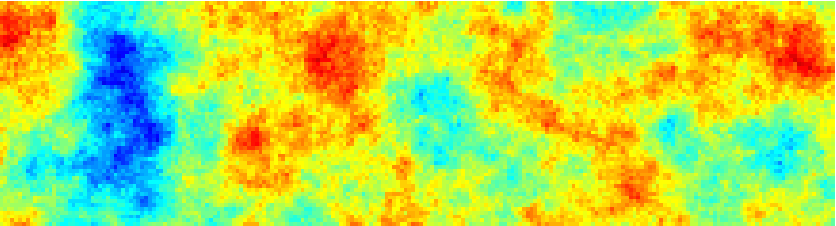
\includegraphics[width=\textwidth]{figures/perm_tarbert_layer-0.png}
\caption{Permeability}
\label{fig:perm_tarbert_layer-0}
\end{subfigure}
\caption{}
\label{fig:tarbert_layer-0}
\end{figure}

%%%%% 60 by 60 %%%%%%%
\subsubsection{60 m by 60 m comments}

\begin{figure}[!ht]
\centering
\tikzsetnextfilename{tarbert_2D_m-0_1}
\begin{subfigure}[b]{0.8\textwidth}
\begin{tikzpicture}
    \begin{semilogyaxis}[
            width=0.97\textwidth,
            height=0.26\textheight,
            xlabel={dt~[d]},
            ylabel={CPU time~[s]},
            grid=both,
            ]
        \addplot table[col sep=comma, trim cells=true,x=dt, y expr= \thisrow{cputime}] {datafiles/spe10-cputvsdt-s-r-T-30-m-1-10-dim-60-60-10-60-220-1-perm-i-0-0-0-i-50.data};
        \addplot table[col sep=comma, trim cells=true,x=dt, y expr=\thisrow{cputime}] {datafiles/spe10-cputvsdt-s-t-T-30-m-1-10-dim-60-60-10-60-220-1-perm-i-0-0-0-i-50.data};
        \addplot table[col sep=comma, trim cells=true,x=dt, y expr=\thisrow{cputime}] {datafiles/spe10-cputvsdt-s-a-T-30-m-1-10-dim-60-60-10-60-220-1-perm-i-0-0-0-i-50.data};
        \addplot table[col sep=comma, trim cells=true,x=dt, y expr=\thisrow{cputime}] {datafiles/spe10-cputvsdt-s-b-T-30-m-1-10-dim-60-60-10-60-220-1-perm-i-0-0-0-i-50.data};
        \addplot table[col sep=comma, trim cells=true,x=dt, y expr=\thisrow{cputime}] {datafiles/spe10-cputvsdt-s-i-T-30-m-1-10-dim-60-60-10-60-220-1-perm-i-0-0-0-i-50.data};
        %\addplot table[col sep=comma, trim cells=true,x=dt, y expr=\thisrow{cputime}] {datafiles/spe10-cputvsdt-s-g-T-30-m-1-10-dim-60-60-10-60-220-1-perm-i-0-0-0-i-50.data};
        \legend{RF,TR,TR*,B,R}
    \end{semilogyaxis}
\end{tikzpicture}%
\label{fig:tarbert_2d_viscrat_0_1}
\caption{Viscosity ratio 0.1}
\end{subfigure}%
\vspace{0.3cm}
\tikzsetnextfilename{tarbert_2D_m-1_0}
\begin{subfigure}[b]{0.8\textwidth}
\begin{tikzpicture}
    \begin{semilogyaxis}[
            width=0.97\textwidth,
            height=0.26\textheight,
            xlabel={dt~[d]},
            ylabel={CPU time~[s]},
            grid=both,
            ]
         \addplot table[col sep=comma, trim cells=true,x=dt, y expr= \thisrow{cputime}] {datafiles/spe10-cputvsdt-s-r-T-30-m-1-1-dim-60-60-10-60-220-1-perm-i-0-0-0-i-50.data};
        \addplot table[col sep=comma, trim cells=true,x=dt, y expr= \thisrow{cputime}] {datafiles/spe10-cputvsdt-s-t-T-30-m-1-1-dim-60-60-10-60-220-1-perm-i-0-0-0-i-50.data};
        \addplot table[col sep=comma, trim cells=true,x=dt, y expr= \thisrow{cputime}] {datafiles/spe10-cputvsdt-s-a-T-30-m-1-1-dim-60-60-10-60-220-1-perm-i-0-0-0-i-50.data};
        \addplot table[col sep=comma, trim cells=true,x=dt, y expr= \thisrow{cputime}] {datafiles/spe10-cputvsdt-s-b-T-30-m-1-1-dim-60-60-10-60-220-1-perm-i-0-0-0-i-50.data};
        \addplot table[col sep=comma, trim cells=true,x=dt, y expr= \thisrow{cputime}] {datafiles/spe10-cputvsdt-s-i-T-30-m-1-1-dim-60-60-10-60-220-1-perm-i-0-0-0-i-50.data};
         %\addplot table[col sep=comma, trim cells=true,x=dt, y expr= \thisrow{cputime}] {datafiles/spe10-cputvsdt-s-g-T-30-m-1-1-dim-60-60-10-60-220-1-perm-i-0-0-0-i-50.data};
        \legend{RF,TR,TR*,B,R}
    \end{semilogyaxis}
\end{tikzpicture}%
\label{fig:tarbert_2d_viscrat_1}
\caption{Viscosity ratio 1}
\end{subfigure}%
\vspace{0.3cm}
\tikzsetnextfilename{tarbert_2D_m-10_0}
\begin{subfigure}[b]{0.8\textwidth}
\begin{tikzpicture}
    \begin{semilogyaxis}[
            width=0.97\textwidth,
            height=0.26\textheight,%
            xlabel={dt~[d]},%
            ylabel={CPU time~[s]},
            grid=both,
            ]
         \addplot table[col sep=comma, trim cells=true,x=dt, y expr= \thisrow{cputime}] {datafiles/spe10-cputvsdt-s-r-T-30-m-10-1-dim-60-60-10-60-220-1-perm-i-0-0-0-i-50.data};
        \addplot table[col sep=comma, trim cells=true,x=dt, y expr= \thisrow{cputime}] {datafiles/spe10-cputvsdt-s-t-T-30-m-10-1-dim-60-60-10-60-220-1-perm-i-0-0-0-i-50.data};
        \addplot table[col sep=comma, trim cells=true,x=dt, y expr= \thisrow{cputime}] {datafiles/spe10-cputvsdt-s-a-T-30-m-10-1-dim-60-60-10-60-220-1-perm-i-0-0-0-i-50.data};
        \addplot table[col sep=comma, trim cells=true,x=dt, y expr= \thisrow{cputime}] {datafiles/spe10-cputvsdt-s-b-T-30-m-10-1-dim-60-60-10-60-220-1-perm-i-0-0-0-i-50.data};
        \addplot table[col sep=comma, trim cells=true,x=dt, y expr= \thisrow{cputime}] {datafiles/spe10-cputvsdt-s-i-T-30-m-10-1-dim-60-60-10-60-220-1-perm-i-0-0-0-i-50.data};
        %\addplot table[col sep=comma, trim cells=true,x=dt, y expr= \thisrow{cputime}] {datafiles/spe10-cputvsdt-s-g-T-30-m-10-1-dim-60-60-10-60-220-1-perm-i-0-0-0-i-50.data};
        \legend{RF,TR,TR*,B,R}
    \end{semilogyaxis}
\end{tikzpicture}%
\label{fig:tarbert_2d_viscrat_10}
\caption{Viscosity ratio 10}
\end{subfigure}%
\label{fig:tarbert_2d}
\caption{CPU time per cell versus time step size $\Delta t$. Inhomogeneous permeabilities from the top layer of the Tarbert formation, as shown in Figure \ref{fig:tarbert_layer-0}.}
\end{figure}

\clearpage
%%%%% 10 by 10 %%%%%%%
\subsubsection{10 m by 10 m comments}

Figure \ref{fig:spe10_iterations_perm_i_0_0_0_i_50} shows the total iteration count used when solving case B using the different root finders and for varying $M$. As noted, the iteration count is orders of magnitude larger than for case A with a range from around $9\times 10^4$ up to around $1.5\times 10^7$ iterations. Again the lowest iteration count is obtained by the trust region schemes, with an advantage to the precise trust region method. The other methods also follow the pattern observed in case A, with the Brent method using the most iterations, and the regula falsi and Ridders methods slightly lower. We note that for $\Delta t \lessapprox \unit[30]{d}$ the regula falsi method has a slight advantage, while the Ridders method is better for larger time steps. 

\begin{figure}[!ht]
\tikzsetnextfilename{spe10_iterations_perm_i_0_0_0_m_1_10_i_50_dt_1to30}
\begin{subfigure}[b]{0.49\textwidth} %%%%%%%%%%% M = 0.1 %%%%%%%%%%%%%%
\begin{tikzpicture}
    \pgfplotstablegetrowsof{datafiles/spe10-iterations-s-r-T-400-m-1-10-dim-10-10-60-220-perm-i-0-0-0-i-50.data}
    \pgfmathsetmacro\yfin{\pgfmathresult}
    \pgfmathsetmacro\yini{5}
    \begin{semilogyaxis}[
            width=0.97\textwidth,
            height=0.26\textheight,
            ymin=300000,
            ymax=15600000,
            xlabel={dt~[d]},
            ylabel={\#iterations},
            grid=both,
            skip coords between index={\yini}{\yfin}
            ]
        \addplot table[col sep=comma, trim cells=true,x=dt, y=iterations] {datafiles/spe10-iterations-s-r-T-400-m-1-10-dim-10-10-60-220-perm-i-0-0-0-i-50.data};
        \addplot table[col sep=comma, trim cells=true,x=dt, y=iterations] {datafiles/spe10-iterations-s-t-T-400-m-1-10-dim-10-10-60-220-perm-i-0-0-0-i-50.data};
        \addplot table[col sep=comma, trim cells=true,x=dt, y=iterations] {datafiles/spe10-iterations-s-a-T-400-m-1-10-dim-10-10-60-220-perm-i-0-0-0-i-50.data};
        \addplot table[col sep=comma, trim cells=true,x=dt, y=iterations] {datafiles/spe10-iterations-s-b-T-400-m-1-10-dim-10-10-60-220-perm-i-0-0-0-i-50.data};
        \addplot table[col sep=comma, trim cells=true,x=dt, y=iterations] {datafiles/spe10-iterations-s-i-T-400-m-1-10-dim-10-10-60-220-perm-i-0-0-0-i-50.data};
        \legend{RF,TR,TR*,B,R}
    \end{semilogyaxis}
\end{tikzpicture}%
\caption{$M =0.1$} \label{fig:spe10_iterations_perm_i_0_0_0_m_1_10_i_50_dt_1to30}
\end{subfigure}%
~
\tikzsetnextfilename{spe10_iterations_perm_i_0_0_0_m_1_10_i_50_dt_40to150}
\begin{subfigure}[b]{0.49\textwidth}
\begin{tikzpicture}
    \pgfplotstablegetrowsof{datafiles/spe10-iterations-s-r-T-400-m-1-10-dim-10-10-60-220-perm-i-0-0-0-i-50.data}
    \pgfmathsetmacro\yfin{5}
    \pgfmathsetmacro\yini{0}
    \begin{semilogyaxis}[
            width=0.97\textwidth,
            height=0.26\textheight,
            ymin=90000,
            ymax=1000000,
            xlabel={dt~[d]},
            ylabel={\#iterations},
            grid=both,
            skip coords between index={\yini}{\yfin}
            ]
        \addplot table[col sep=comma, trim cells=true,x=dt, y=iterations] {datafiles/spe10-iterations-s-r-T-400-m-1-10-dim-10-10-60-220-perm-i-0-0-0-i-50.data};
        \addplot table[col sep=comma, trim cells=true,x=dt, y=iterations] {datafiles/spe10-iterations-s-t-T-400-m-1-10-dim-10-10-60-220-perm-i-0-0-0-i-50.data};
        \addplot table[col sep=comma, trim cells=true,x=dt, y=iterations] {datafiles/spe10-iterations-s-a-T-400-m-1-10-dim-10-10-60-220-perm-i-0-0-0-i-50.data};
        \addplot table[col sep=comma, trim cells=true,x=dt, y=iterations] {datafiles/spe10-iterations-s-b-T-400-m-1-10-dim-10-10-60-220-perm-i-0-0-0-i-50.data};
        \addplot table[col sep=comma, trim cells=true,x=dt, y=iterations] {datafiles/spe10-iterations-s-i-T-400-m-1-10-dim-10-10-60-220-perm-i-0-0-0-i-50.data};
        %\legend{RF,TR,TR*,B,R}
    \end{semilogyaxis}
\end{tikzpicture}%
\caption{$M =0.1$} \label{fig:spe10_iterations_perm_i_0_0_0_m_1_10_i_50_dt_40to150}
\end{subfigure}%
\vspace{0.3cm} %%%%%%%%%%% M = 1 %%%%%%%%%%%%%%
\tikzsetnextfilename{spe10_iterations_perm_i_0_0_0_m_1_1_i_50_dt_1to30}
\begin{subfigure}[b]{0.49\textwidth}
\begin{tikzpicture}
    \pgfplotstablegetrowsof{datafiles/spe10-iterations-s-r-T-400-m-1-10-dim-10-10-60-220-perm-i-0-0-0-i-50.data}
    \pgfmathsetmacro\yfin{\pgfmathresult}
    \pgfmathsetmacro\yini{5}
    \begin{semilogyaxis}[
            width=0.97\textwidth,
            height=0.26\textheight,
            ymin=190000,
            ymax=11500000,
            xlabel={dt~[d]},
            ylabel={\#iterations},
            grid=both,
            skip coords between index={\yini}{\yfin}
            ]
         \addplot table[col sep=comma, trim cells=true,x=dt, y=iterations] {datafiles/spe10-iterations-s-r-T-400-m-1-1-dim-10-10-60-220-perm-i-0-0-0-i-50.data};
        \addplot table[col sep=comma, trim cells=true,x=dt, y=iterations] {datafiles/spe10-iterations-s-t-T-400-m-1-1-dim-10-10-60-220-perm-i-0-0-0-i-50.data};
        \addplot table[col sep=comma, trim cells=true,x=dt, y=iterations] {datafiles/spe10-iterations-s-a-T-400-m-1-1-dim-10-10-60-220-perm-i-0-0-0-i-50.data};
        \addplot table[col sep=comma, trim cells=true,x=dt, y=iterations] {datafiles/spe10-iterations-s-b-T-400-m-1-1-dim-10-10-60-220-perm-i-0-0-0-i-50.data};
        \addplot table[col sep=comma, trim cells=true,x=dt, y=iterations] {datafiles/spe10-iterations-s-i-T-400-m-1-1-dim-10-10-60-220-perm-i-0-0-0-i-50.data};
        \legend{RF,TR,TR*,B,R}
    \end{semilogyaxis}
\end{tikzpicture}%
\caption{$M =1$} \label{fig:spe10_iterations_perm_i_0_0_0_m_1_1_i_50_dt_1to30}
\end{subfigure}%
~
\tikzsetnextfilename{spe10_iterations_perm_i_0_0_0_m_1_1_i_50_dt_40to150}
\begin{subfigure}[b]{0.49\textwidth}
\begin{tikzpicture}
    \pgfplotstablegetrowsof{datafiles/spe10-iterations-s-r-T-400-m-1-10-dim-10-10-60-220-perm-i-0-0-0-i-50.data}
    \pgfmathsetmacro\yfin{5}
    \pgfmathsetmacro\yini{0}
    \begin{semilogyaxis}[
            width=0.97\textwidth,
            height=0.26\textheight,
            ymin=86000,
            ymax=1000000,
            xlabel={dt~[d]},
            ylabel={\#iterations},
            grid=both,
            skip coords between index={\yini}{\yfin}
            ]
         \addplot table[col sep=comma, trim cells=true,x=dt, y=iterations] {datafiles/spe10-iterations-s-r-T-400-m-1-1-dim-10-10-60-220-perm-i-0-0-0-i-50.data};
        \addplot table[col sep=comma, trim cells=true,x=dt, y=iterations] {datafiles/spe10-iterations-s-t-T-400-m-1-1-dim-10-10-60-220-perm-i-0-0-0-i-50.data};
        \addplot table[col sep=comma, trim cells=true,x=dt, y=iterations] {datafiles/spe10-iterations-s-a-T-400-m-1-1-dim-10-10-60-220-perm-i-0-0-0-i-50.data};
        \addplot table[col sep=comma, trim cells=true,x=dt, y=iterations] {datafiles/spe10-iterations-s-b-T-400-m-1-1-dim-10-10-60-220-perm-i-0-0-0-i-50.data};
        \addplot table[col sep=comma, trim cells=true,x=dt, y=iterations] {datafiles/spe10-iterations-s-i-T-400-m-1-1-dim-10-10-60-220-perm-i-0-0-0-i-50.data};
        %\legend{RF,TR,TR*,B,R}
    \end{semilogyaxis}
\end{tikzpicture}%
\caption{$M =1$} \label{fig:spe10_iterations_perm_i_0_0_0_m_1_1_i_50_dt_40to150}
\end{subfigure}%
\vspace{0.3cm} %%%%%%%%%%% M = 10 %%%%%%%%%%%%%%
\tikzsetnextfilename{spe10_iterations_perm_i_0_0_0_m_10_1_i_50_dt_1to30}
\begin{subfigure}[b]{0.49\textwidth}
\begin{tikzpicture}
    \pgfplotstablegetrowsof{datafiles/spe10-iterations-s-r-T-400-m-1-10-dim-10-10-60-220-perm-i-0-0-0-i-50.data}
    \pgfmathsetmacro\yfin{\pgfmathresult}
    \pgfmathsetmacro\yini{5}
    \begin{semilogyaxis}[
            width=0.97\textwidth,
            height=0.26\textheight,
            ymin=200000,
            ymax=10000000,
            xlabel={dt~[d]},
            ylabel={\#iterations},
            grid=both,
            skip coords between index={\yini}{\yfin}
            ]
         \addplot table[col sep=comma, trim cells=true,x=dt, y=iterations] {datafiles/spe10-iterations-s-r-T-400-m-10-1-dim-10-10-60-220-perm-i-0-0-0-i-50.data};
        \addplot table[col sep=comma, trim cells=true,x=dt, y=iterations] {datafiles/spe10-iterations-s-t-T-400-m-10-1-dim-10-10-60-220-perm-i-0-0-0-i-50.data};
        \addplot table[col sep=comma, trim cells=true,x=dt, y=iterations] {datafiles/spe10-iterations-s-a-T-400-m-10-1-dim-10-10-60-220-perm-i-0-0-0-i-50.data};
        \addplot table[col sep=comma, trim cells=true,x=dt, y=iterations] {datafiles/spe10-iterations-s-b-T-400-m-10-1-dim-10-10-60-220-perm-i-0-0-0-i-50.data};
        \addplot table[col sep=comma, trim cells=true,x=dt, y=iterations] {datafiles/spe10-iterations-s-i-T-400-m-10-1-dim-10-10-60-220-perm-i-0-0-0-i-50.data};
        \legend{RF,TR,TR*,B,R}
    \end{semilogyaxis}
\end{tikzpicture}%
\caption{$M =10$} \label{fig:spe10_iterations_perm_i_0_0_0_m_10_1_i_50_dt_1to30}
\end{subfigure}%
~
\tikzsetnextfilename{spe10_iterations_perm_i_0_0_0_m_10_1_i_50_dt_40to150}
\begin{subfigure}[b]{0.49\textwidth}
\begin{tikzpicture}
    \pgfplotstablegetrowsof{datafiles/spe10-iterations-s-r-T-400-m-1-10-dim-10-10-60-220-perm-i-0-0-0-i-50.data}
    \pgfmathsetmacro\yfin{5}
    \pgfmathsetmacro\yini{0}
    \begin{semilogyaxis}[
            width=0.97\textwidth,
            height=0.26\textheight,
            ymin=64000,
            ymax=1000000,
            xlabel={dt~[d]},
            ylabel={\#iterations},
            grid=both,
            skip coords between index={\yini}{\yfin}
            ]
         \addplot table[col sep=comma, trim cells=true,x=dt, y=iterations] {datafiles/spe10-iterations-s-r-T-400-m-10-1-dim-10-10-60-220-perm-i-0-0-0-i-50.data};
        \addplot table[col sep=comma, trim cells=true,x=dt, y=iterations] {datafiles/spe10-iterations-s-t-T-400-m-10-1-dim-10-10-60-220-perm-i-0-0-0-i-50.data};
        \addplot table[col sep=comma, trim cells=true,x=dt, y=iterations] {datafiles/spe10-iterations-s-a-T-400-m-10-1-dim-10-10-60-220-perm-i-0-0-0-i-50.data};
        \addplot table[col sep=comma, trim cells=true,x=dt, y=iterations] {datafiles/spe10-iterations-s-b-T-400-m-10-1-dim-10-10-60-220-perm-i-0-0-0-i-50.data};
        \addplot table[col sep=comma, trim cells=true,x=dt, y=iterations] {datafiles/spe10-iterations-s-i-T-400-m-10-1-dim-10-10-60-220-perm-i-0-0-0-i-50.data};
        %\legend{RF,TR,TR*,B,R}
    \end{semilogyaxis}
\end{tikzpicture}%
\caption{$M =10$} \label{fig:spe10_iterations_perm_i_0_0_0_m_10_1_i_50_dt_40to150}
\end{subfigure}%
\caption{\#iterations used to solve case B, Section \ref{section:caseB}, for varying root finders, time steps and viscosity ratios.}
\label{fig:spe10_iterations_perm_i_0_0_0_i_50}
\end{figure}%
%
%\begin{figure}[!ht]
%\centering
%\tikzsetnextfilename{spe10_iterations_perm_i_0_0_0_m_1_10_i_50}
%\begin{subfigure}[b]{0.8\textwidth}
%\begin{tikzpicture}
%    \pgfplotstablegetrowsof{datafiles/spe10-iterations-s-r-T-400-m-1-10-dim-10-10-60-220-perm-i-0-0-0-i-50.data}
%    \pgfmathsetmacro\yfin{\pgfmathresult - 4}
%    \pgfmathsetmacro\yini{0}
%    \begin{semilogyaxis}[
%            width=0.97\textwidth,
%            height=0.26\textheight,
%            ymin=40000,
%            ymax=30000000,
%            xlabel={dt~[d]},
%            ylabel={\#iterations},
%            grid=both,
%            ]
%        \addplot table[col sep=comma, trim cells=true,x=dt, y=iterations] {datafiles/spe10-iterations-s-r-T-400-m-1-10-dim-10-10-60-220-perm-i-0-0-0-i-50.data};
%        \addplot table[col sep=comma, trim cells=true,x=dt, y=iterations] {datafiles/spe10-iterations-s-t-T-400-m-1-10-dim-10-10-60-220-perm-i-0-0-0-i-50.data};
%        \addplot table[col sep=comma, trim cells=true,x=dt, y=iterations] {datafiles/spe10-iterations-s-a-T-400-m-1-10-dim-10-10-60-220-perm-i-0-0-0-i-50.data};
%        \addplot table[col sep=comma, trim cells=true,x=dt, y=iterations] {datafiles/spe10-iterations-s-b-T-400-m-1-10-dim-10-10-60-220-perm-i-0-0-0-i-50.data};
%        \addplot table[col sep=comma, trim cells=true,x=dt, y=iterations] {datafiles/spe10-iterations-s-i-T-400-m-1-10-dim-10-10-60-220-perm-i-0-0-0-i-50.data};
%                %\addplot table[col sep=comma, trim cells=true,x=dt, y=iterations] {datafiles/spe10-iterations-s-g-T-400-m-1-10-dim-10-10-60-220-perm-i-0-0-0-i-50.data};
%        \legend{RF,TR,TR*,B,R}
%    \end{semilogyaxis}
%\end{tikzpicture}%
%\caption{$M =0.1$} \label{fig:spe10_iterations_perm_i_0_0_0_m_1_10_i_50}
%\end{subfigure}%
%\vspace{0.3cm}
%\centering
%\tikzsetnextfilename{spe10_iterations_perm_i_0_0_0_m_1_1_i_50}
%\begin{subfigure}[b]{0.8\textwidth}
%\begin{tikzpicture}
%    \begin{semilogyaxis}[
%            width=0.97\textwidth,
%            height=0.26\textheight,
%            ymin=40000,
%            ymax=30000000,
%            xlabel={dt~[d]},
%            ylabel={\#iterations},
%            grid=both,
%            ]
%         \addplot table[col sep=comma, trim cells=true,x=dt, y=iterations] {datafiles/spe10-iterations-s-r-T-400-m-1-1-dim-10-10-60-220-perm-i-0-0-0-i-50.data};
%        \addplot table[col sep=comma, trim cells=true,x=dt, y=iterations] {datafiles/spe10-iterations-s-t-T-400-m-1-1-dim-10-10-60-220-perm-i-0-0-0-i-50.data};
%        \addplot table[col sep=comma, trim cells=true,x=dt, y=iterations] {datafiles/spe10-iterations-s-a-T-400-m-1-1-dim-10-10-60-220-perm-i-0-0-0-i-50.data};
%        \addplot table[col sep=comma, trim cells=true,x=dt, y=iterations] {datafiles/spe10-iterations-s-b-T-400-m-1-1-dim-10-10-60-220-perm-i-0-0-0-i-50.data};
%        \addplot table[col sep=comma, trim cells=true,x=dt, y=iterations] {datafiles/spe10-iterations-s-i-T-400-m-1-1-dim-10-10-60-220-perm-i-0-0-0-i-50.data};
%                %\addplot table[col sep=comma, trim cells=true,x=dt, y=iterations] {datafiles/spe10-iterations-s-g-T-400-m-1-1-dim-10-10-60-220-perm-i-0-0-0-i-50.data};
%        \legend{RF,TR,TR*,B,R}
%    \end{semilogyaxis}
%\end{tikzpicture}%
%\caption{$M =1$} \label{fig:spe10_iterations_perm_i_0_0_0_m_1_1_i_50}
%\end{subfigure}%
%\vspace{0.3cm}
%\centering
%\tikzsetnextfilename{spe10_iterations_perm_i_0_0_0_m_10_1_i_50}
%\begin{subfigure}[b]{0.8\textwidth}
%\begin{tikzpicture}
%    \begin{semilogyaxis}[
%            width=0.97\textwidth,
%            height=0.26\textheight,
%            ymin=40000,
%            ymax=30000000,
%            xlabel={dt~[d]},
%            ylabel={\#iterations},
%            grid=both,
%            ]
%         \addplot table[col sep=comma, trim cells=true,x=dt, y=iterations] {datafiles/spe10-iterations-s-r-T-400-m-10-1-dim-10-10-60-220-perm-i-0-0-0-i-50.data};
%        \addplot table[col sep=comma, trim cells=true,x=dt, y=iterations] {datafiles/spe10-iterations-s-t-T-400-m-10-1-dim-10-10-60-220-perm-i-0-0-0-i-50.data};
%        \addplot table[col sep=comma, trim cells=true,x=dt, y=iterations] {datafiles/spe10-iterations-s-a-T-400-m-10-1-dim-10-10-60-220-perm-i-0-0-0-i-50.data};
%        \addplot table[col sep=comma, trim cells=true,x=dt, y=iterations] {datafiles/spe10-iterations-s-b-T-400-m-10-1-dim-10-10-60-220-perm-i-0-0-0-i-50.data};
%        \addplot table[col sep=comma, trim cells=true,x=dt, y=iterations] {datafiles/spe10-iterations-s-i-T-400-m-10-1-dim-10-10-60-220-perm-i-0-0-0-i-50.data};
%                %\addplot table[col sep=comma, trim cells=true,x=dt, y=iterations] {datafiles/spe10-iterations-s-g-T-400-m-10-1-dim-10-10-60-220-perm-i-0-0-0-i-50.data};
%        \legend{RF,TR,TR*,B,R}
%    \end{semilogyaxis}
%\end{tikzpicture}%
%\caption{$M =10$} \label{fig:spe10_iterations_perm_i_0_0_0_m_10_1_i_50}
%\end{subfigure}%
%\caption{\#iterations used to solve the Q5 problem, Section \ref{section:caseA}, for varying root finders, time steps and viscosity ratios.}
%\label{fig:spe10_iterations_perm_i_0_0_0_i_50}
%\end{figure}
%\begin{figure}[!ht]
\centering
\tikzsetnextfilename{spe10_cputime_perm_i_0_0_0_m_1_10_i_50}
\begin{subfigure}[b]{0.8\textwidth}
\begin{tikzpicture}
    \begin{semilogyaxis}[
            width=0.97\textwidth,
            height=0.26\textheight,
            xlabel={dt~[d]},
            ylabel={CPU time~[s]},
            grid=both,
            ]
        \addplot table[col sep=comma, trim cells=true,x=dt, y=cputime] {datafiles/spe10-cputvsdt-s-r-T-400-m-1-10-dim-10-10-60-220-perm-i-0-0-0-i-50.data};
        \addplot table[col sep=comma, trim cells=true,x=dt, y=cputime] {datafiles/spe10-cputvsdt-s-t-T-400-m-1-10-dim-10-10-60-220-perm-i-0-0-0-i-50.data};
        \addplot table[col sep=comma, trim cells=true,x=dt, y=cputime] {datafiles/spe10-cputvsdt-s-a-T-400-m-1-10-dim-10-10-60-220-perm-i-0-0-0-i-50.data};
        \addplot table[col sep=comma, trim cells=true,x=dt, y=cputime] {datafiles/spe10-cputvsdt-s-b-T-400-m-1-10-dim-10-10-60-220-perm-i-0-0-0-i-50.data};
        \addplot table[col sep=comma, trim cells=true,x=dt, y=cputime] {datafiles/spe10-cputvsdt-s-i-T-400-m-1-10-dim-10-10-60-220-perm-i-0-0-0-i-50.data};                
        \legend{RF,TR,TR*,B,R}
    \end{semilogyaxis}
\end{tikzpicture}%
\caption{$M =0.1$} \label{fig:spe10_cputime_perm_i_0_0_0_m_1_10_i_50}
\end{subfigure}%
\vspace{0.3cm}
\centering
\tikzsetnextfilename{spe10_cputime_perm_i_0_0_0_m_1_1_i_50}
\begin{subfigure}[b]{0.8\textwidth}
\begin{tikzpicture}
    \begin{semilogyaxis}[
            width=0.97\textwidth,
            height=0.26\textheight,
            xlabel={dt~[d]},
            ylabel={CPU time~[s]},
            grid=both,
            ]
         \addplot table[col sep=comma, trim cells=true,x=dt, y=cputime] {datafiles/spe10-cputvsdt-s-r-T-400-m-1-1-dim-10-10-60-220-perm-i-0-0-0-i-50.data};
        \addplot table[col sep=comma, trim cells=true,x=dt, y=cputime] {datafiles/spe10-cputvsdt-s-t-T-400-m-1-1-dim-10-10-60-220-perm-i-0-0-0-i-50.data};
        \addplot table[col sep=comma, trim cells=true,x=dt, y=cputime] {datafiles/spe10-cputvsdt-s-a-T-400-m-1-1-dim-10-10-60-220-perm-i-0-0-0-i-50.data};
        \addplot table[col sep=comma, trim cells=true,x=dt, y=cputime] {datafiles/spe10-cputvsdt-s-b-T-400-m-1-1-dim-10-10-60-220-perm-i-0-0-0-i-50.data};
        \addplot table[col sep=comma, trim cells=true,x=dt, y=cputime] {datafiles/spe10-cputvsdt-s-i-T-400-m-1-1-dim-10-10-60-220-perm-i-0-0-0-i-50.data};
        \legend{RF,TR,TR*,B,R}
    \end{semilogyaxis}
\end{tikzpicture}%
\caption{$M =1$} \label{fig:spe10_cputime_perm_i_0_0_0_m_1_1_i_50}
\end{subfigure}%
\vspace{0.3cm}
\centering
\tikzsetnextfilename{spe10_cputime_perm_i_0_0_0_m_10_1_i_50}
\begin{subfigure}[b]{0.8\textwidth}
\begin{tikzpicture}
    \begin{semilogyaxis}[
            width=0.97\textwidth,
            height=0.26\textheight,
            xlabel={dt~[d]},
            ylabel={CPU time~[s]},
            grid=both,
            ]
         \addplot table[col sep=comma, trim cells=true,x=dt, y=cputime] {datafiles/spe10-cputvsdt-s-r-T-400-m-10-1-dim-10-10-60-220-perm-i-0-0-0-i-50.data};
        \addplot table[col sep=comma, trim cells=true,x=dt, y=cputime] {datafiles/spe10-cputvsdt-s-t-T-400-m-10-1-dim-10-10-60-220-perm-i-0-0-0-i-50.data};
        \addplot table[col sep=comma, trim cells=true,x=dt, y=cputime] {datafiles/spe10-cputvsdt-s-a-T-400-m-10-1-dim-10-10-60-220-perm-i-0-0-0-i-50.data};
        \addplot table[col sep=comma, trim cells=true,x=dt, y=cputime] {datafiles/spe10-cputvsdt-s-b-T-400-m-10-1-dim-10-10-60-220-perm-i-0-0-0-i-50.data};
        \addplot table[col sep=comma, trim cells=true,x=dt, y=cputime] {datafiles/spe10-cputvsdt-s-i-T-400-m-10-1-dim-10-10-60-220-perm-i-0-0-0-i-50.data};
        \legend{RF,TR,TR*,B,R}
    \end{semilogyaxis}
\end{tikzpicture}%
\caption{$M =10$} \label{fig:spe10_cputime_perm_i_0_0_0_m_10_1_i_50}
\end{subfigure}%
\caption{CPU time used to solve case B, Section \ref{section:caseB}, for varying root finders, time steps and viscosity ratios.}
\label{fig:spe10_cputime_perm_i_0_0_0_i_50}
\end{figure}

\clearpage
%%%%%%%%%%%%%%%%  UPPER NESS 2D %%%%%%%%%%%%%%%%%%%
\subsection{Case C: Upper Ness 2D}
\label{section:caseC}
\todoinline{Comment the results from Upper Ness 2D}
Figure \ref{fig:spe10_perm} indicates that the Upper Ness formation has more severe local permeability variations compared to the Tarbert formation. These large local variations appear as \todo{show the effects of large local perm. gradients on the residual.}. Again we want to investigate how the various root finders perform on this special case, choosing the $\unit[360]{m}\times \unit[180]{m}$ region starting at $(x,y) = (0,0)$ in layer 45 of the SPE10 data set for the permeabilities.

\begin{figure}[ht]
\centering
\begin{subfigure}{0.49\textwidth}
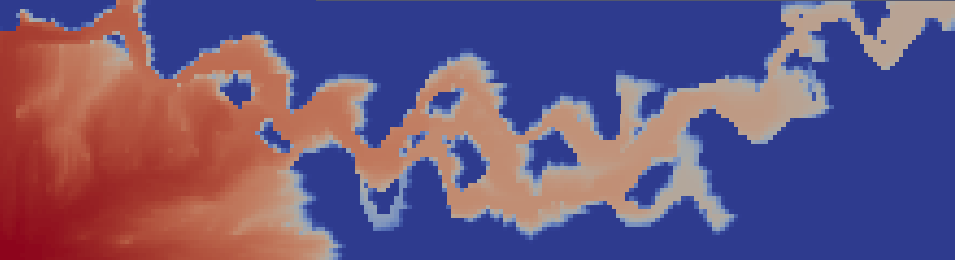
\includegraphics[width=\textwidth]{figures/saturation_upperness_layer-35.png}
\caption{Saturation at $T = \unit[30]{d}$}
\label{fig:saturation_upperness_layer-35}
\end{subfigure}
~
\begin{subfigure}{0.49\textwidth}
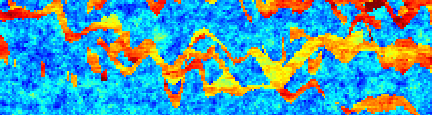
\includegraphics[width=\textwidth]{figures/perm_upperness_layer-35.png}
\caption{Permeability}
\label{fig:perm_upperness_layer-35}
\end{subfigure}
\caption{}
\label{fig:upperness_layer-35}
\end{figure}

%%%%% 60 by 60 %%%%%%%
\subsubsection{60 m by 60 m comments}

\begin{figure}[!ht]
\centering
\tikzsetnextfilename{upperness_2D_m-0_1}
\begin{subfigure}[b]{0.8\textwidth}
\begin{tikzpicture}
    \begin{semilogyaxis}[
            width=0.97\textwidth,
            height=0.26\textheight,
            xlabel={dt~[d]},
            ylabel={CPU time~[s]},
            grid=both,
            ]
        \addplot table[col sep=comma, trim cells=true,x=dt, y expr= \thisrow{cputime}] {datafiles/spe10-cputvsdt-s-r-T-30-m-1-10-dim-60-60-10-60-220-1-perm-i-36-0-0-i-50.data};
        \addplot table[col sep=comma, trim cells=true,x=dt, y expr= \thisrow{cputime}] {datafiles/spe10-cputvsdt-s-t-T-30-m-1-10-dim-60-60-10-60-220-1-perm-i-36-0-0-i-50.data};
        \addplot table[col sep=comma, trim cells=true,x=dt, y expr= \thisrow{cputime}] {datafiles/spe10-cputvsdt-s-a-T-30-m-1-10-dim-60-60-10-60-220-1-perm-i-36-0-0-i-50.data};
        \addplot table[col sep=comma, trim cells=true,x=dt, y expr= \thisrow{cputime}] {datafiles/spe10-cputvsdt-s-b-T-30-m-1-10-dim-60-60-10-60-220-1-perm-i-36-0-0-i-50.data};
        \addplot table[col sep=comma, trim cells=true,x=dt, y expr= \thisrow{cputime}] {datafiles/spe10-cputvsdt-s-i-T-30-m-1-10-dim-60-60-10-60-220-1-perm-i-36-0-0-i-50.data};
                \addplot table[col sep=comma, trim cells=true,x=dt, y expr= \thisrow{cputime}] {datafiles/spe10-cputvsdt-s-g-T-30-m-1-10-dim-60-60-10-60-220-1-perm-i-36-0-0-i-50.data};
        \legend{RF,TR,TR*,B,R,GN}
    \end{semilogyaxis}
\end{tikzpicture}%
\label{fig:tarbert_2d_viscrat_0_1}
\caption{Viscosity ratio 0.1}
\end{subfigure}%
\vspace{0.3cm}
\tikzsetnextfilename{upperness_2D_m-1_0}
\begin{subfigure}[b]{0.8\textwidth}
\begin{tikzpicture}
    \begin{semilogyaxis}[
            width=0.97\textwidth,
            height=0.26\textheight,
            xlabel={dt~[d]},
            ylabel={CPU time~[s]},
            grid=both,
            ]
         \addplot table[col sep=comma, trim cells=true,x=dt, y expr= \thisrow{cputime}] {datafiles/spe10-cputvsdt-s-r-T-30-m-1-1-dim-60-60-10-60-220-1-perm-i-36-0-0-i-50.data};
        \addplot table[col sep=comma, trim cells=true,x=dt, y expr= \thisrow{cputime}] {datafiles/spe10-cputvsdt-s-t-T-30-m-1-1-dim-60-60-10-60-220-1-perm-i-36-0-0-i-50.data};
        \addplot table[col sep=comma, trim cells=true,x=dt, y expr= \thisrow{cputime}] {datafiles/spe10-cputvsdt-s-a-T-30-m-1-1-dim-60-60-10-60-220-1-perm-i-36-0-0-i-50.data};
        \addplot table[col sep=comma, trim cells=true,x=dt, y expr= \thisrow{cputime}] {datafiles/spe10-cputvsdt-s-b-T-30-m-1-1-dim-60-60-10-60-220-1-perm-i-36-0-0-i-50.data};
        \addplot table[col sep=comma, trim cells=true,x=dt, y expr= \thisrow{cputime}] {datafiles/spe10-cputvsdt-s-i-T-30-m-1-1-dim-60-60-10-60-220-1-perm-i-36-0-0-i-50.data};
                \addplot table[col sep=comma, trim cells=true,x=dt, y expr= \thisrow{cputime}] {datafiles/spe10-cputvsdt-s-g-T-30-m-1-1-dim-60-60-10-60-220-1-perm-i-36-0-0-i-50.data};
        \legend{RF,TR,TR*,B,R,GN}
    \end{semilogyaxis}
\end{tikzpicture}%
\label{fig:tarbert_2d_viscrat_1}
\caption{Viscosity ratio 1}
\end{subfigure}%
\vspace{0.3cm}
\tikzsetnextfilename{upperness_2D_m-10_0}
\begin{subfigure}[b]{0.8\textwidth}
\begin{tikzpicture}
    \begin{semilogyaxis}[
            width=0.97\textwidth,
            height=0.26\textheight,%
            xlabel={dt~[d]},%
            ylabel={CPU time~[s]},
            grid=both,
            ]
         \addplot table[col sep=comma, trim cells=true,x=dt, y expr= \thisrow{cputime}] {datafiles/spe10-cputvsdt-s-r-T-30-m-10-1-dim-60-60-10-60-220-1-perm-i-36-0-0-i-50.data};
        \addplot table[col sep=comma, trim cells=true,x=dt, y expr= \thisrow{cputime}] {datafiles/spe10-cputvsdt-s-t-T-30-m-10-1-dim-60-60-10-60-220-1-perm-i-36-0-0-i-50.data};
        \addplot table[col sep=comma, trim cells=true,x=dt, y expr= \thisrow{cputime}] {datafiles/spe10-cputvsdt-s-a-T-30-m-10-1-dim-60-60-10-60-220-1-perm-i-36-0-0-i-50.data};
        \addplot table[col sep=comma, trim cells=true,x=dt, y expr= \thisrow{cputime}] {datafiles/spe10-cputvsdt-s-b-T-30-m-10-1-dim-60-60-10-60-220-1-perm-i-36-0-0-i-50.data};
        \addplot table[col sep=comma, trim cells=true,x=dt, y expr= \thisrow{cputime}] {datafiles/spe10-cputvsdt-s-i-T-30-m-10-1-dim-60-60-10-60-220-1-perm-i-36-0-0-i-50.data};
        \addplot table[col sep=comma, trim cells=true,x=dt, y expr= \thisrow{cputime}] {datafiles/spe10-cputvsdt-s-g-T-30-m-10-1-dim-60-60-10-60-220-1-perm-i-36-0-0-i-50.data};
        \legend{RF,TR,TR*,B,R,GN}
    \end{semilogyaxis}
\end{tikzpicture}%
\label{fig:tarbert_2d_viscrat_10}
\caption{Viscosity ratio 10}
\end{subfigure}%
\label{fig:tarbert_2d}
\caption{CPU time per cell versus time step size $\Delta t$. Inhomogeneous permeabilities from the top layer of the Tarbert formation, as shown in Figure \ref{fig:tarbert_layer-0}.}
\end{figure}
\begin{figure}[!ht]
\centering
\tikzsetnextfilename{upperness_2D_m-0_1}
\begin{subfigure}[b]{0.8\textwidth}
\begin{tikzpicture}
    \begin{semilogyaxis}[
            width=0.97\textwidth,
            height=0.26\textheight,
            xlabel={dt~[d]},
            ylabel={CPU time~[s]},
            grid=both,
            ]
        \addplot table[col sep=comma, trim cells=true,x=dt, y expr= \thisrow{cputime}] {datafiles/spe10-cputvsdt-s-r-T-30-m-1-10-dim-60-60-10-60-220-1-perm-i-36-0-0-i-50.data};
        \addplot table[col sep=comma, trim cells=true,x=dt, y expr= \thisrow{cputime}] {datafiles/spe10-cputvsdt-s-t-T-30-m-1-10-dim-60-60-10-60-220-1-perm-i-36-0-0-i-50.data};
        \addplot table[col sep=comma, trim cells=true,x=dt, y expr= \thisrow{cputime}] {datafiles/spe10-cputvsdt-s-a-T-30-m-1-10-dim-60-60-10-60-220-1-perm-i-36-0-0-i-50.data};
        \addplot table[col sep=comma, trim cells=true,x=dt, y expr= \thisrow{cputime}] {datafiles/spe10-cputvsdt-s-b-T-30-m-1-10-dim-60-60-10-60-220-1-perm-i-36-0-0-i-50.data};
        \addplot table[col sep=comma, trim cells=true,x=dt, y expr= \thisrow{cputime}] {datafiles/spe10-cputvsdt-s-i-T-30-m-1-10-dim-60-60-10-60-220-1-perm-i-36-0-0-i-50.data};
                \addplot table[col sep=comma, trim cells=true,x=dt, y expr= \thisrow{cputime}] {datafiles/spe10-cputvsdt-s-g-T-30-m-1-10-dim-60-60-10-60-220-1-perm-i-36-0-0-i-50.data};
        \legend{RF,TR,TR*,B,R,GN}
    \end{semilogyaxis}
\end{tikzpicture}%
\label{fig:tarbert_2d_viscrat_0_1}
\caption{Viscosity ratio 0.1}
\end{subfigure}%
\vspace{0.3cm}
\tikzsetnextfilename{upperness_2D_m-1_0}
\begin{subfigure}[b]{0.8\textwidth}
\begin{tikzpicture}
    \begin{semilogyaxis}[
            width=0.97\textwidth,
            height=0.26\textheight,
            xlabel={dt~[d]},
            ylabel={CPU time~[s]},
            grid=both,
            ]
         \addplot table[col sep=comma, trim cells=true,x=dt, y expr= \thisrow{cputime}] {datafiles/spe10-cputvsdt-s-r-T-30-m-1-1-dim-60-60-10-60-220-1-perm-i-36-0-0-i-50.data};
        \addplot table[col sep=comma, trim cells=true,x=dt, y expr= \thisrow{cputime}] {datafiles/spe10-cputvsdt-s-t-T-30-m-1-1-dim-60-60-10-60-220-1-perm-i-36-0-0-i-50.data};
        \addplot table[col sep=comma, trim cells=true,x=dt, y expr= \thisrow{cputime}] {datafiles/spe10-cputvsdt-s-a-T-30-m-1-1-dim-60-60-10-60-220-1-perm-i-36-0-0-i-50.data};
        \addplot table[col sep=comma, trim cells=true,x=dt, y expr= \thisrow{cputime}] {datafiles/spe10-cputvsdt-s-b-T-30-m-1-1-dim-60-60-10-60-220-1-perm-i-36-0-0-i-50.data};
        \addplot table[col sep=comma, trim cells=true,x=dt, y expr= \thisrow{cputime}] {datafiles/spe10-cputvsdt-s-i-T-30-m-1-1-dim-60-60-10-60-220-1-perm-i-36-0-0-i-50.data};
                \addplot table[col sep=comma, trim cells=true,x=dt, y expr= \thisrow{cputime}] {datafiles/spe10-cputvsdt-s-g-T-30-m-1-1-dim-60-60-10-60-220-1-perm-i-36-0-0-i-50.data};
        \legend{RF,TR,TR*,B,R,GN}
    \end{semilogyaxis}
\end{tikzpicture}%
\label{fig:tarbert_2d_viscrat_1}
\caption{Viscosity ratio 1}
\end{subfigure}%
\vspace{0.3cm}
\tikzsetnextfilename{upperness_2D_m-10_0}
\begin{subfigure}[b]{0.8\textwidth}
\begin{tikzpicture}
    \begin{semilogyaxis}[
            width=0.97\textwidth,
            height=0.26\textheight,%
            xlabel={dt~[d]},%
            ylabel={CPU time~[s]},
            grid=both,
            ]
         \addplot table[col sep=comma, trim cells=true,x=dt, y expr= \thisrow{cputime}] {datafiles/spe10-cputvsdt-s-r-T-30-m-10-1-dim-60-60-10-60-220-1-perm-i-36-0-0-i-50.data};
        \addplot table[col sep=comma, trim cells=true,x=dt, y expr= \thisrow{cputime}] {datafiles/spe10-cputvsdt-s-t-T-30-m-10-1-dim-60-60-10-60-220-1-perm-i-36-0-0-i-50.data};
        \addplot table[col sep=comma, trim cells=true,x=dt, y expr= \thisrow{cputime}] {datafiles/spe10-cputvsdt-s-a-T-30-m-10-1-dim-60-60-10-60-220-1-perm-i-36-0-0-i-50.data};
        \addplot table[col sep=comma, trim cells=true,x=dt, y expr= \thisrow{cputime}] {datafiles/spe10-cputvsdt-s-b-T-30-m-10-1-dim-60-60-10-60-220-1-perm-i-36-0-0-i-50.data};
        \addplot table[col sep=comma, trim cells=true,x=dt, y expr= \thisrow{cputime}] {datafiles/spe10-cputvsdt-s-i-T-30-m-10-1-dim-60-60-10-60-220-1-perm-i-36-0-0-i-50.data};
        \addplot table[col sep=comma, trim cells=true,x=dt, y expr= \thisrow{cputime}] {datafiles/spe10-cputvsdt-s-g-T-30-m-10-1-dim-60-60-10-60-220-1-perm-i-36-0-0-i-50.data};
        \legend{RF,TR,TR*,B,R,GN}
    \end{semilogyaxis}
\end{tikzpicture}%
\label{fig:tarbert_2d_viscrat_10}
\caption{Viscosity ratio 10}
\end{subfigure}%
\label{fig:tarbert_2d}
\caption{CPU time per cell versus time step size $\Delta t$. Inhomogeneous permeabilities from the top layer of the Tarbert formation, as shown in Figure \ref{fig:tarbert_layer-0}.}
\end{figure}

\clearpage
%%%%% 10 by 10 %%%%%%%
\subsubsection{10 m by 10 m comments}

\begin{figure}[!ht]
\tikzsetnextfilename{spe10_iterations_perm_i_36_0_0_m_1_10_i_50_dt_1to30}
\begin{subfigure}[b]{0.49\textwidth} %%%%%%%%%%% M = 0.1 %%%%%%%%%%%%%%
\begin{tikzpicture}
    \pgfplotstablegetrowsof{datafiles/spe10-iterations-s-r-T-400-m-1-10-dim-10-10-60-220-perm-i-36-0-0-i-50.data}
    \pgfmathsetmacro\yfin{\pgfmathresult}
    \pgfmathsetmacro\yini{5}
    \begin{semilogyaxis}[
            width=0.97\textwidth,
            height=0.26\textheight,
            ymin=300000,
            ymax=15600000,
            xlabel={dt~[days]},
            ylabel={\#iterations},
            grid=major,
            skip coords between index={\yini}{\yfin}
            ]
        \addplot table[col sep=comma, trim cells=true,x=dt, y=iterations] {datafiles/spe10-iterations-s-r-T-400-m-1-10-dim-10-10-60-220-perm-i-36-0-0-i-50.data};
        \addplot table[col sep=comma, trim cells=true,x=dt, y=iterations] {datafiles/spe10-iterations-s-t-T-400-m-1-10-dim-10-10-60-220-perm-i-36-0-0-i-50.data};
        \addplot table[col sep=comma, trim cells=true,x=dt, y=iterations] {datafiles/spe10-iterations-s-a-T-400-m-1-10-dim-10-10-60-220-perm-i-36-0-0-i-50.data};
        \addplot table[col sep=comma, trim cells=true,x=dt, y=iterations] {datafiles/spe10-iterations-s-b-T-400-m-1-10-dim-10-10-60-220-perm-i-36-0-0-i-50.data};
        \addplot table[col sep=comma, trim cells=true,x=dt, y=iterations] {datafiles/spe10-iterations-s-i-T-400-m-1-10-dim-10-10-60-220-perm-i-36-0-0-i-50.data};
        \legend{RF,TR,TR*,B,R}
    \end{semilogyaxis}
\end{tikzpicture}%
\caption{$M =0.1$} \label{fig:spe10_iterations_perm_i_36_0_0_m_1_10_i_50_dt_1to30}
\end{subfigure}%
~
\tikzsetnextfilename{spe10_iterations_perm_i_36_0_0_m_1_10_i_50_dt_40to150}
\begin{subfigure}[b]{0.49\textwidth}
\begin{tikzpicture}
    \pgfplotstablegetrowsof{datafiles/spe10-iterations-s-r-T-400-m-1-10-dim-10-10-60-220-perm-i-36-0-0-i-50.data}
    \pgfmathsetmacro\yfin{5}
    \pgfmathsetmacro\yini{0}
    \begin{semilogyaxis}[
            width=0.97\textwidth,
            height=0.26\textheight,
            ymin=70000,
            ymax=1000000,
            xlabel={dt~[days]},
            ylabel={\#iterations},
            grid=major,
            skip coords between index={\yini}{\yfin}
            ]
        \addplot table[col sep=comma, trim cells=true,x=dt, y=iterations] {datafiles/spe10-iterations-s-r-T-400-m-1-10-dim-10-10-60-220-perm-i-36-0-0-i-50.data};
        \addplot table[col sep=comma, trim cells=true,x=dt, y=iterations] {datafiles/spe10-iterations-s-t-T-400-m-1-10-dim-10-10-60-220-perm-i-36-0-0-i-50.data};
        \addplot table[col sep=comma, trim cells=true,x=dt, y=iterations] {datafiles/spe10-iterations-s-a-T-400-m-1-10-dim-10-10-60-220-perm-i-36-0-0-i-50.data};
        \addplot table[col sep=comma, trim cells=true,x=dt, y=iterations] {datafiles/spe10-iterations-s-b-T-400-m-1-10-dim-10-10-60-220-perm-i-36-0-0-i-50.data};
        \addplot table[col sep=comma, trim cells=true,x=dt, y=iterations] {datafiles/spe10-iterations-s-i-T-400-m-1-10-dim-10-10-60-220-perm-i-36-0-0-i-50.data};
        %\legend{RF,TR,TR*,B,R}
    \end{semilogyaxis}
\end{tikzpicture}%
\caption{$M =0.1$} \label{fig:spe10_iterations_perm_i_36_0_0_m_1_10_i_50_dt_40to150}
\end{subfigure}%
\vspace{0.3cm} %%%%%%%%%%% M = 1 %%%%%%%%%%%%%%
\tikzsetnextfilename{spe10_iterations_perm_i_36_0_0_m_1_1_i_50_dt_1to30}
\begin{subfigure}[b]{0.49\textwidth}
\begin{tikzpicture}
    \pgfplotstablegetrowsof{datafiles/spe10-iterations-s-r-T-400-m-1-10-dim-10-10-60-220-perm-i-36-0-0-i-50.data}
    \pgfmathsetmacro\yfin{\pgfmathresult}
    \pgfmathsetmacro\yini{5}
    \begin{semilogyaxis}[
            width=0.97\textwidth,
            height=0.26\textheight,
            ymin=190000,
            ymax=11500000,
            xlabel={dt~[days]},
            ylabel={\#iterations},
            grid=major,
            skip coords between index={\yini}{\yfin}
            ]
         \addplot table[col sep=comma, trim cells=true,x=dt, y=iterations] {datafiles/spe10-iterations-s-r-T-400-m-1-1-dim-10-10-60-220-perm-i-36-0-0-i-50.data};
        \addplot table[col sep=comma, trim cells=true,x=dt, y=iterations] {datafiles/spe10-iterations-s-t-T-400-m-1-1-dim-10-10-60-220-perm-i-36-0-0-i-50.data};
        \addplot table[col sep=comma, trim cells=true,x=dt, y=iterations] {datafiles/spe10-iterations-s-a-T-400-m-1-1-dim-10-10-60-220-perm-i-36-0-0-i-50.data};
        \addplot table[col sep=comma, trim cells=true,x=dt, y=iterations] {datafiles/spe10-iterations-s-b-T-400-m-1-1-dim-10-10-60-220-perm-i-36-0-0-i-50.data};
        \addplot table[col sep=comma, trim cells=true,x=dt, y=iterations] {datafiles/spe10-iterations-s-i-T-400-m-1-1-dim-10-10-60-220-perm-i-36-0-0-i-50.data};
        \legend{RF,TR,TR*,B,R}
    \end{semilogyaxis}
\end{tikzpicture}%
\caption{$M =1$} \label{fig:spe10_iterations_perm_i_36_0_0_m_1_1_i_50_dt_1to30}
\end{subfigure}%
~
\tikzsetnextfilename{spe10_iterations_perm_i_36_0_0_m_1_1_i_50_dt_40to150}
\begin{subfigure}[b]{0.49\textwidth}
\begin{tikzpicture}
    \pgfplotstablegetrowsof{datafiles/spe10-iterations-s-r-T-400-m-1-10-dim-10-10-60-220-perm-i-36-0-0-i-50.data}
    \pgfmathsetmacro\yfin{5}
    \pgfmathsetmacro\yini{0}
    \begin{semilogyaxis}[
            width=0.97\textwidth,
            height=0.26\textheight,
            ymin=60000,
            ymax=1000000,
            xlabel={dt~[days]},
            ylabel={\#iterations},
            grid=major,
            skip coords between index={\yini}{\yfin}
            ]
         \addplot table[col sep=comma, trim cells=true,x=dt, y=iterations] {datafiles/spe10-iterations-s-r-T-400-m-1-1-dim-10-10-60-220-perm-i-36-0-0-i-50.data};
        \addplot table[col sep=comma, trim cells=true,x=dt, y=iterations] {datafiles/spe10-iterations-s-t-T-400-m-1-1-dim-10-10-60-220-perm-i-36-0-0-i-50.data};
        \addplot table[col sep=comma, trim cells=true,x=dt, y=iterations] {datafiles/spe10-iterations-s-a-T-400-m-1-1-dim-10-10-60-220-perm-i-36-0-0-i-50.data};
        \addplot table[col sep=comma, trim cells=true,x=dt, y=iterations] {datafiles/spe10-iterations-s-b-T-400-m-1-1-dim-10-10-60-220-perm-i-36-0-0-i-50.data};
        \addplot table[col sep=comma, trim cells=true,x=dt, y=iterations] {datafiles/spe10-iterations-s-i-T-400-m-1-1-dim-10-10-60-220-perm-i-36-0-0-i-50.data};
        %\legend{RF,TR,TR*,B,R}
    \end{semilogyaxis}
\end{tikzpicture}%
\caption{$M =1$} \label{fig:spe10_iterations_perm_i_36_0_0_m_1_1_i_50_dt_40to150}
\end{subfigure}%
\vspace{0.3cm} %%%%%%%%%%% M = 10 %%%%%%%%%%%%%%
\tikzsetnextfilename{spe10_iterations_perm_i_36_0_0_m_10_1_i_50_dt_1to30}
\begin{subfigure}[b]{0.49\textwidth}
\begin{tikzpicture}
    \pgfplotstablegetrowsof{datafiles/spe10-iterations-s-r-T-400-m-1-10-dim-10-10-60-220-perm-i-36-0-0-i-50.data}
    \pgfmathsetmacro\yfin{\pgfmathresult}
    \pgfmathsetmacro\yini{5}
    \begin{semilogyaxis}[
            width=0.97\textwidth,
            height=0.26\textheight,
            ymin=200000,
            ymax=10000000,
            xlabel={dt~[days]},
            ylabel={\#iterations},
            grid=major,
            skip coords between index={\yini}{\yfin}
            ]
         \addplot table[col sep=comma, trim cells=true,x=dt, y=iterations] {datafiles/spe10-iterations-s-r-T-400-m-10-1-dim-10-10-60-220-perm-i-36-0-0-i-50.data};
        \addplot table[col sep=comma, trim cells=true,x=dt, y=iterations] {datafiles/spe10-iterations-s-t-T-400-m-10-1-dim-10-10-60-220-perm-i-36-0-0-i-50.data};
        \addplot table[col sep=comma, trim cells=true,x=dt, y=iterations] {datafiles/spe10-iterations-s-a-T-400-m-10-1-dim-10-10-60-220-perm-i-36-0-0-i-50.data};
        \addplot table[col sep=comma, trim cells=true,x=dt, y=iterations] {datafiles/spe10-iterations-s-b-T-400-m-10-1-dim-10-10-60-220-perm-i-36-0-0-i-50.data};
        \addplot table[col sep=comma, trim cells=true,x=dt, y=iterations] {datafiles/spe10-iterations-s-i-T-400-m-10-1-dim-10-10-60-220-perm-i-36-0-0-i-50.data};
        \legend{RF,TR,TR*,B,R}
    \end{semilogyaxis}
\end{tikzpicture}%
\caption{$M =10$} \label{fig:spe10_iterations_perm_i_36_0_0_m_10_1_i_50_dt_1to30}
\end{subfigure}%
~
\tikzsetnextfilename{spe10_iterations_perm_i_36_0_0_m_10_1_i_50_dt_40to150}
\begin{subfigure}[b]{0.49\textwidth}
\begin{tikzpicture}
    \pgfplotstablegetrowsof{datafiles/spe10-iterations-s-r-T-400-m-1-10-dim-10-10-60-220-perm-i-36-0-0-i-50.data}
    \pgfmathsetmacro\yfin{5}
    \pgfmathsetmacro\yini{0}
    \begin{semilogyaxis}[
            width=0.97\textwidth,
            height=0.26\textheight,
            ymin=64000,
            ymax=1000000,
            xlabel={dt~[days]},
            ylabel={\#iterations},
            grid=major,
            skip coords between index={\yini}{\yfin}
            ]
         \addplot table[col sep=comma, trim cells=true,x=dt, y=iterations] {datafiles/spe10-iterations-s-r-T-400-m-10-1-dim-10-10-60-220-perm-i-36-0-0-i-50.data};
        \addplot table[col sep=comma, trim cells=true,x=dt, y=iterations] {datafiles/spe10-iterations-s-t-T-400-m-10-1-dim-10-10-60-220-perm-i-36-0-0-i-50.data};
        \addplot table[col sep=comma, trim cells=true,x=dt, y=iterations] {datafiles/spe10-iterations-s-a-T-400-m-10-1-dim-10-10-60-220-perm-i-36-0-0-i-50.data};
        \addplot table[col sep=comma, trim cells=true,x=dt, y=iterations] {datafiles/spe10-iterations-s-b-T-400-m-10-1-dim-10-10-60-220-perm-i-36-0-0-i-50.data};
        \addplot table[col sep=comma, trim cells=true,x=dt, y=iterations] {datafiles/spe10-iterations-s-i-T-400-m-10-1-dim-10-10-60-220-perm-i-36-0-0-i-50.data};
        %\legend{RF,TR,TR*,B,R}
    \end{semilogyaxis}
\end{tikzpicture}%
\caption{$M =10$} \label{fig:spe10_iterations_perm_i_36_0_0_m_10_1_i_50_dt_40to150}
\end{subfigure}%
\caption{\#iterations used to solve case B, Section \ref{section:caseB}, for varying root finders, time steps and viscosity ratios.}
\label{fig:spe10_iterations_perm_i_36_0_0_i_50}
\end{figure}%
%
%\begin{figure}[!ht]
%\centering
%\tikzsetnextfilename{spe10_iterations_perm_i_36_0_0_m_1_10_i_50}
%\begin{subfigure}[b]{0.8\textwidth}
%\begin{tikzpicture}
%    \pgfplotstablegetrowsof{datafiles/spe10-iterations-s-r-T-400-m-1-10-dim-10-10-60-220-perm-i-36-0-0-i-50.data}
%    \pgfmathsetmacro\yfin{\pgfmathresult - 4}
%    \pgfmathsetmacro\yini{0}
%    \begin{semilogyaxis}[
%            width=0.97\textwidth,
%            height=0.26\textheight,
%            ymin=40000,
%            ymax=30000000,
%            xlabel={dt~[days]},
%            ylabel={\#iterations},
%            grid=major,
%            ]
%        \addplot table[col sep=comma, trim cells=true,x=dt, y=iterations] {datafiles/spe10-iterations-s-r-T-400-m-1-10-dim-10-10-60-220-perm-i-36-0-0-i-50.data};
%        \addplot table[col sep=comma, trim cells=true,x=dt, y=iterations] {datafiles/spe10-iterations-s-t-T-400-m-1-10-dim-10-10-60-220-perm-i-36-0-0-i-50.data};
%        \addplot table[col sep=comma, trim cells=true,x=dt, y=iterations] {datafiles/spe10-iterations-s-a-T-400-m-1-10-dim-10-10-60-220-perm-i-36-0-0-i-50.data};
%        \addplot table[col sep=comma, trim cells=true,x=dt, y=iterations] {datafiles/spe10-iterations-s-b-T-400-m-1-10-dim-10-10-60-220-perm-i-36-0-0-i-50.data};
%        \addplot table[col sep=comma, trim cells=true,x=dt, y=iterations] {datafiles/spe10-iterations-s-i-T-400-m-1-10-dim-10-10-60-220-perm-i-36-0-0-i-50.data};
%                %\addplot table[col sep=comma, trim cells=true,x=dt, y=iterations] {datafiles/spe10-iterations-s-g-T-400-m-1-10-dim-10-10-60-220-perm-i-36-0-0-i-50.data};
%        \legend{RF,TR,TR*,B,R}
%    \end{semilogyaxis}
%\end{tikzpicture}%
%\caption{$M =0.1$} \label{fig:spe10_iterations_perm_i_36_0_0_m_1_10_i_50}
%\end{subfigure}%
%\vspace{0.3cm}
%\centering
%\tikzsetnextfilename{spe10_iterations_perm_i_36_0_0_m_1_1_i_50}
%\begin{subfigure}[b]{0.8\textwidth}
%\begin{tikzpicture}
%    \begin{semilogyaxis}[
%            width=0.97\textwidth,
%            height=0.26\textheight,
%            ymin=40000,
%            ymax=30000000,
%            xlabel={dt~[days]},
%            ylabel={\#iterations},
%            grid=major,
%            ]
%         \addplot table[col sep=comma, trim cells=true,x=dt, y=iterations] {datafiles/spe10-iterations-s-r-T-400-m-1-1-dim-10-10-60-220-perm-i-36-0-0-i-50.data};
%        \addplot table[col sep=comma, trim cells=true,x=dt, y=iterations] {datafiles/spe10-iterations-s-t-T-400-m-1-1-dim-10-10-60-220-perm-i-36-0-0-i-50.data};
%        \addplot table[col sep=comma, trim cells=true,x=dt, y=iterations] {datafiles/spe10-iterations-s-a-T-400-m-1-1-dim-10-10-60-220-perm-i-36-0-0-i-50.data};
%        \addplot table[col sep=comma, trim cells=true,x=dt, y=iterations] {datafiles/spe10-iterations-s-b-T-400-m-1-1-dim-10-10-60-220-perm-i-36-0-0-i-50.data};
%        \addplot table[col sep=comma, trim cells=true,x=dt, y=iterations] {datafiles/spe10-iterations-s-i-T-400-m-1-1-dim-10-10-60-220-perm-i-36-0-0-i-50.data};
%                %\addplot table[col sep=comma, trim cells=true,x=dt, y=iterations] {datafiles/spe10-iterations-s-g-T-400-m-1-1-dim-10-10-60-220-perm-i-36-0-0-i-50.data};
%        \legend{RF,TR,TR*,B,R}
%    \end{semilogyaxis}
%\end{tikzpicture}%
%\caption{$M =1$} \label{fig:spe10_iterations_perm_i_36_0_0_m_1_1_i_50}
%\end{subfigure}%
%\vspace{0.3cm}
%\centering
%\tikzsetnextfilename{spe10_iterations_perm_i_36_0_0_m_10_1_i_50}
%\begin{subfigure}[b]{0.8\textwidth}
%\begin{tikzpicture}
%    \begin{semilogyaxis}[
%            width=0.97\textwidth,
%            height=0.26\textheight,
%            ymin=40000,
%            ymax=30000000,
%            xlabel={dt~[days]},
%            ylabel={\#iterations},
%            grid=major,
%            ]
%         \addplot table[col sep=comma, trim cells=true,x=dt, y=iterations] {datafiles/spe10-iterations-s-r-T-400-m-10-1-dim-10-10-60-220-perm-i-36-0-0-i-50.data};
%        \addplot table[col sep=comma, trim cells=true,x=dt, y=iterations] {datafiles/spe10-iterations-s-t-T-400-m-10-1-dim-10-10-60-220-perm-i-36-0-0-i-50.data};
%        \addplot table[col sep=comma, trim cells=true,x=dt, y=iterations] {datafiles/spe10-iterations-s-a-T-400-m-10-1-dim-10-10-60-220-perm-i-36-0-0-i-50.data};
%        \addplot table[col sep=comma, trim cells=true,x=dt, y=iterations] {datafiles/spe10-iterations-s-b-T-400-m-10-1-dim-10-10-60-220-perm-i-36-0-0-i-50.data};
%        \addplot table[col sep=comma, trim cells=true,x=dt, y=iterations] {datafiles/spe10-iterations-s-i-T-400-m-10-1-dim-10-10-60-220-perm-i-36-0-0-i-50.data};
%                %\addplot table[col sep=comma, trim cells=true,x=dt, y=iterations] {datafiles/spe10-iterations-s-g-T-400-m-10-1-dim-10-10-60-220-perm-i-36-0-0-i-50.data};
%        \legend{RF,TR,TR*,B,R}
%    \end{semilogyaxis}
%\end{tikzpicture}%
%\caption{$M =10$} \label{fig:spe10_iterations_perm_i_36_0_0_m_10_1_i_50}
%\end{subfigure}%
%\caption{\#iterations used to solve the Q5 problem, Section \ref{section:caseA}, for varying root finders, time steps and viscosity ratios.}
%\label{fig:spe10_iterations_perm_i_36_0_0_i_50}
%\end{figure}
%\begin{figure}[!ht]
\centering
\tikzsetnextfilename{spe10_cputime_perm_i_36_0_0_m_1_10_i_50}
\begin{subfigure}[b]{0.8\textwidth}
\begin{tikzpicture}
    \begin{semilogyaxis}[
            width=0.97\textwidth,
            height=0.26\textheight,
            xlabel={dt~[d]},
            ylabel={CPU time~[s]},
            grid=both,
            ]
        \addplot table[col sep=comma, trim cells=true,x=dt, y=cputime] {datafiles/spe10-cputvsdt-s-r-T-400-m-1-10-dim-10-10-60-220-perm-i-36-0-0-i-50.data};
        \addplot table[col sep=comma, trim cells=true,x=dt, y=cputime] {datafiles/spe10-cputvsdt-s-t-T-400-m-1-10-dim-10-10-60-220-perm-i-36-0-0-i-50.data};
        \addplot table[col sep=comma, trim cells=true,x=dt, y=cputime] {datafiles/spe10-cputvsdt-s-a-T-400-m-1-10-dim-10-10-60-220-perm-i-36-0-0-i-50.data};
        \addplot table[col sep=comma, trim cells=true,x=dt, y=cputime] {datafiles/spe10-cputvsdt-s-b-T-400-m-1-10-dim-10-10-60-220-perm-i-36-0-0-i-50.data};
        \addplot table[col sep=comma, trim cells=true,x=dt, y=cputime] {datafiles/spe10-cputvsdt-s-i-T-400-m-1-10-dim-10-10-60-220-perm-i-36-0-0-i-50.data};
        \legend{RF,TR,TR*,B,R}
    \end{semilogyaxis}
\end{tikzpicture}%
\caption{$M =0.1$} \label{fig:spe10_cputime_perm_i_36_0_0_m_1_10_i_50}
\end{subfigure}%
\vspace{0.3cm}
\centering
\tikzsetnextfilename{spe10_cputime_perm_i_36_0_0_m_1_1_i_50}
\begin{subfigure}[b]{0.8\textwidth}
\begin{tikzpicture}
    \begin{semilogyaxis}[
            width=0.97\textwidth,
            height=0.26\textheight,
            xlabel={dt~[d]},
            ylabel={CPU time~[s]},
            grid=both,
            ]
         \addplot table[col sep=comma, trim cells=true,x=dt, y=cputime] {datafiles/spe10-cputvsdt-s-r-T-400-m-1-1-dim-10-10-60-220-perm-i-36-0-0-i-50.data};
        \addplot table[col sep=comma, trim cells=true,x=dt, y=cputime] {datafiles/spe10-cputvsdt-s-t-T-400-m-1-1-dim-10-10-60-220-perm-i-36-0-0-i-50.data};
        \addplot table[col sep=comma, trim cells=true,x=dt, y=cputime] {datafiles/spe10-cputvsdt-s-a-T-400-m-1-1-dim-10-10-60-220-perm-i-36-0-0-i-50.data};
        \addplot table[col sep=comma, trim cells=true,x=dt, y=cputime] {datafiles/spe10-cputvsdt-s-b-T-400-m-1-1-dim-10-10-60-220-perm-i-36-0-0-i-50.data};
        \addplot table[col sep=comma, trim cells=true,x=dt, y=cputime] {datafiles/spe10-cputvsdt-s-i-T-400-m-1-1-dim-10-10-60-220-perm-i-36-0-0-i-50.data};
        \legend{RF,TR,TR*,B,R}
    \end{semilogyaxis}
\end{tikzpicture}%
\caption{$M =1$} \label{fig:spe10_cputime_perm_i_36_0_0_m_1_1_i_50}
\end{subfigure}%
\vspace{0.3cm}
\centering
\tikzsetnextfilename{spe10_cputime_perm_i_36_0_0_m_10_1_i_50}
\begin{subfigure}[b]{0.8\textwidth}
\begin{tikzpicture}
    \begin{semilogyaxis}[
            width=0.97\textwidth,
            height=0.26\textheight,
            xlabel={dt~[d]},
            ylabel={CPU time~[s]},
            grid=both,
            ]
         \addplot table[col sep=comma, trim cells=true,x=dt, y=cputime] {datafiles/spe10-cputvsdt-s-r-T-400-m-10-1-dim-10-10-60-220-perm-i-36-0-0-i-50.data};
        \addplot table[col sep=comma, trim cells=true,x=dt, y=cputime] {datafiles/spe10-cputvsdt-s-t-T-400-m-10-1-dim-10-10-60-220-perm-i-36-0-0-i-50.data};
        \addplot table[col sep=comma, trim cells=true,x=dt, y=cputime] {datafiles/spe10-cputvsdt-s-a-T-400-m-10-1-dim-10-10-60-220-perm-i-36-0-0-i-50.data};
        \addplot table[col sep=comma, trim cells=true,x=dt, y=cputime] {datafiles/spe10-cputvsdt-s-b-T-400-m-10-1-dim-10-10-60-220-perm-i-36-0-0-i-50.data};
        \addplot table[col sep=comma, trim cells=true,x=dt, y=cputime] {datafiles/spe10-cputvsdt-s-i-T-400-m-10-1-dim-10-10-60-220-perm-i-36-0-0-i-50.data};
        \legend{RF,TR,TR*,B,R}
    \end{semilogyaxis}
\end{tikzpicture}%
\caption{$M =10$} \label{fig:spe10_cputime_perm_i_36_0_0_m_10_1_i_50}
\end{subfigure}%
\caption{CPU time used to solve case C, Section \ref{section:caseC}, for varying root finders, time steps and viscosity ratios.}
\label{fig:spe10_cputime_perm_i_36_0_0_i_50}
\end{figure}

\clearpage
%%%%%%%%%%%%%%%% TARBERT - 3D %%%%%%%%%%%%%%%%%%%
\subsection{Case D: Tarbert 3D}
\label{section:caseD}

\todoinline{Permeability/saturation plot for Tarbert 3D}
\todoinline{Run Tarbert 3D with gravity - cputime}
\todoinline{Run Tarbert 3D with gravity - iterations}

\clearpage
%%%%%%%%%%%%%%%%  UPPER NESS - 3D %%%%%%%%%%%%%%%%%%%
\subsection{Case E: Upper Ness 3D}
\label{section:caseE}

\todoinline{Permeability/saturation plot for Upper Ness 3D}
\todoinline{Run Upper Ness 3D with gravity - cputime}
\todoinline{Run Upper Ness 3D with gravity - iterations}

\clearpage
%%%%%%%%%%%%%%%% CONVERGENCE TESTS %%%%%%%%%%%%%%%%%%
\section{Convergence Tests}
\label{section:numerical_results_convergence_tests}
The efficiency of the numerical methods in terms of convergence speed can highlight the properties of the numerical procedures. We again \todo{Comment briefly on the properties of the viscosity residual when it is introduced.} observe that the form of the viscosity dominated residual from Equation (\ref{eq:residual_two_phase_transport}) is determined by five parameters; the initial saturation in the cell, $S_V^{n}$, the time step to pore volume ratio $\tau = \frac{\Delta t}{m(V)\phi_V}$, the flux out of the cell $q_o$, the flux into the cell $q_i$, and finally the viscosity ratio $M$ as defined in Equation (\ref{eq:viscosity_ratio}), held constant at $M = 1$. Note that the cell saturation from the previous time step is used as initial guess for the root finders. Figures \ref{fig:conv_res_in_0_05_out_0_05} through \ref{fig:conv_res_in_0_5_out_0_8} shows a number of different convergence and residual plots obtained by varying these parameters. 

Figure \ref{fig:conv_res_in_0_05_out_0_05} is obtained with incoming flux at $\unitfrac[0.05]{m^3}{s}$ and outgoing flux at $\unitfrac[0.05]{m^3}{s}$. Note that $\tau = \unitfrac[6]{s}{m^3}$. Under the circumstances the residuals are fairly linear, and the initial guess $S_0$ is close to the root. The number of iterations for all tested root finders decreases when $S_0$ is increased. We also note that the Newton-like methods converge faster than the other methods. This plot indicates that for small flux values the initial guess strongly influences the residual bringing the root close to $S_0$. with a stronger effect for larger $S_0$. 

Setting the incoming flux to $\unitfrac[0.35]{m^3}{s}$ and the outgoing flux to $\unitfrac[0.35]{m^3}{s}$ we obtain Figure \ref{fig:conv_res_in_0_35_out_0_35}. The residual plots shown a stronger non-linear influence, a fact reflected in the increased iteration count. $S_0$ still influences the residual, but to a lesser extent. Again we observe that large initial guesses generally leads to a lower iteration count. The Newton-like method are, together with Ridders, the best performers.

Moving on the even larger flux values, we set the incoming flux to $\unitfrac[0.5]{m^3}{s}$ and the outgoing flux to $\unitfrac[0.8]{m^3}{s}$. Figure \ref{fig:conv_res_in_0_5_out_0_8} shows the resulting plots. The trend from the previous plots continues, in that the initial guess has less influence on the performance of the root finders, on average. Interesting exceptions are the Newton-like methods. They perform significantly better in terms of iteration count when the initial guess is close, in contrast with the other methods. We also note that the initial has very little influence on the position of the root.

\begin{figure}[!ht]
\centering
\begin{subfigure}[b]{0.49\textwidth}
\begin{tikzpicture}
    \begin{semilogyaxis}[
            width=0.97\textwidth,
            height=0.3\textheight,
            xlabel={\#steps},
            ylabel={error},
            grid=both,
            legend pos=south west,
            ]
        \addplot table[col sep=comma, trim cells=true,x=iter, y=y] {testcasedatafiles/convergence2-s-r-M-1_000000-dtpv-6_000000-in--0_050000-out-0_050000-s0-0_100000.data};
        \addplot table[col sep=comma, trim cells=true,x=iter, y=y] {testcasedatafiles/convergence2-s-t-M-1_000000-dtpv-6_000000-in--0_050000-out-0_050000-s0-0_100000.data};
        \addplot table[col sep=comma, trim cells=true,x=iter, y=y] {testcasedatafiles/convergence2-s-a-M-1_000000-dtpv-6_000000-in--0_050000-out-0_050000-s0-0_100000.data};
        \addplot table[col sep=comma, trim cells=true,x=iter, y=y] {testcasedatafiles/convergence2-s-b-M-1_000000-dtpv-6_000000-in--0_050000-out-0_050000-s0-0_100000.data};
        \addplot table[col sep=comma, trim cells=true,x=iter, y=y] {testcasedatafiles/convergence2-s-i-M-1_000000-dtpv-6_000000-in--0_050000-out-0_050000-s0-0_100000.data};
        \addplot table[col sep=comma, trim cells=true,x=iter, y=y] {testcasedatafiles/convergence2-s-g-M-1_000000-dtpv-6_000000-in--0_050000-out-0_050000-s0-0_100000.data};
        \legend{RF,TR,TR*,B,R,GN}
    \end{semilogyaxis}
\end{tikzpicture}%
\caption{$S_0 = 0.1$}
\label{fig:convergence_in_0_05_out_0_05_s0_0_1}
\end{subfigure}%
\begin{subfigure}[b]{0.49\textwidth}
\begin{tikzpicture}
    \begin{axis}[
            width=0.97\textwidth,
            height=0.3\textheight,
            xlabel={S~[d]},
            ylabel={R(S)},
            grid=both,
            legend pos=north west,
            ]
        \addplot table[mark=none, col sep=comma, trim cells=true,x=s, y=Rs] {testcasedatafiles/residual-convergence2-s-r-M-1_000000-dtpv-6_000000-in--0_050000-out-0_050000-s0-0_100000.data};
        \addplot table[mark=none, col sep=comma, trim cells=true,x=s, y=dRs] {testcasedatafiles/residual-convergence2-s-r-M-1_000000-dtpv-6_000000-in--0_050000-out-0_050000-s0-0_100000.data};
            \legend{$R(S)$,$\partial_S R(S)$}
    \end{axis}
\end{tikzpicture}%
\caption{$S_0 = 0.1$}
\label{fig:residual_in_0_05_out_0_05_s0_0_1}
\end{subfigure}%
\vspace{0.4cm}
\begin{subfigure}[b]{0.49\textwidth}
\begin{tikzpicture}
    \begin{semilogyaxis}[
            width=0.97\textwidth,
            height=0.3\textheight,
            xlabel={\#steps},
            ylabel={error},
            grid=both,
            legend pos=south west,
            ]
        \addplot table[col sep=comma, trim cells=true,x=iter, y=y] {testcasedatafiles/convergence2-s-r-M-1_000000-dtpv-6_000000-in--0_050000-out-0_050000-s0-0_500000.data};
        \addplot table[col sep=comma, trim cells=true,x=iter, y=y] {testcasedatafiles/convergence2-s-t-M-1_000000-dtpv-6_000000-in--0_050000-out-0_050000-s0-0_500000.data};
        \addplot table[col sep=comma, trim cells=true,x=iter, y=y] {testcasedatafiles/convergence2-s-a-M-1_000000-dtpv-6_000000-in--0_050000-out-0_050000-s0-0_500000.data};
        \addplot table[col sep=comma, trim cells=true,x=iter, y=y] {testcasedatafiles/convergence2-s-b-M-1_000000-dtpv-6_000000-in--0_050000-out-0_050000-s0-0_500000.data};
        \addplot table[col sep=comma, trim cells=true,x=iter, y=y] {testcasedatafiles/convergence2-s-i-M-1_000000-dtpv-6_000000-in--0_050000-out-0_050000-s0-0_500000.data};
        \addplot table[col sep=comma, trim cells=true,x=iter, y=y] {testcasedatafiles/convergence2-s-g-M-1_000000-dtpv-6_000000-in--0_050000-out-0_050000-s0-0_500000.data};
        \legend{RF,TR,TR*,B,R,GN}
    \end{semilogyaxis}
\end{tikzpicture}%
\caption{$S_0 = 0.5$}
\label{fig:convergence_in_0_05_out_0_05_s0_0_5}
\end{subfigure}%
\begin{subfigure}[b]{0.49\textwidth}
\begin{tikzpicture}
    \begin{axis}[
            width=0.97\textwidth,
            height=0.3\textheight,
            xlabel={S},
            ylabel={$R(S)$},
            grid=both,
            legend pos=north west,
            ]
        \addplot table[mark=none, col sep=comma, trim cells=true,x=s, y=Rs] {testcasedatafiles/residual-convergence2-s-r-M-1_000000-dtpv-6_000000-in--0_050000-out-0_050000-s0-0_500000.data};
        \addplot table[mark=none, col sep=comma, trim cells=true,x=s, y=dRs] {testcasedatafiles/residual-convergence2-s-r-M-1_000000-dtpv-6_000000-in--0_050000-out-0_050000-s0-0_500000.data};
            \legend{$R(S)$,$\partial_S R(S)$}
    \end{axis}
\end{tikzpicture}%
\caption{$S_0 = 0.5$}
\label{fig:residual_in_0_05_out_0_05_s0_0_5}
\end{subfigure}%
\vspace{0.4cm}
\begin{subfigure}[b]{0.49\textwidth}
\begin{tikzpicture}
    \begin{semilogyaxis}[
            width=0.97\textwidth,
            height=0.3\textheight,
            xlabel={\#steps},
            ylabel={error},
            grid=both,
            legend pos=south west,
            ]
        \addplot table[col sep=comma, trim cells=true,x=iter, y=y] {testcasedatafiles/convergence2-s-r-M-1_000000-dtpv-6_000000-in--0_050000-out-0_050000-s0-0_900000.data};
        \addplot table[col sep=comma, trim cells=true,x=iter, y=y] {testcasedatafiles/convergence2-s-t-M-1_000000-dtpv-6_000000-in--0_050000-out-0_050000-s0-0_900000.data};
        \addplot table[col sep=comma, trim cells=true,x=iter, y=y] {testcasedatafiles/convergence2-s-a-M-1_000000-dtpv-6_000000-in--0_050000-out-0_050000-s0-0_900000.data};
        \addplot table[col sep=comma, trim cells=true,x=iter, y=y] {testcasedatafiles/convergence2-s-b-M-1_000000-dtpv-6_000000-in--0_050000-out-0_050000-s0-0_900000.data};
        \addplot table[col sep=comma, trim cells=true,x=iter, y=y] {testcasedatafiles/convergence2-s-i-M-1_000000-dtpv-6_000000-in--0_050000-out-0_050000-s0-0_900000.data};
        \addplot table[col sep=comma, trim cells=true,x=iter, y=y] {testcasedatafiles/convergence2-s-g-M-1_000000-dtpv-6_000000-in--0_050000-out-0_050000-s0-0_900000.data};
        \legend{RF,TR,TR*,B,R,GN}
    \end{semilogyaxis}
\end{tikzpicture}%
\caption{$S_0 = 0.9$}
\label{fig:convergence_in_0_05_out_0_05_s0_0_9}
\end{subfigure}%
\begin{subfigure}[b]{0.49\textwidth}
\begin{tikzpicture}
    \begin{axis}[
            width=0.97\textwidth,
            height=0.3\textheight,
            xlabel={S},
            ylabel={$R(S)$},
            grid=both,
            legend pos=north west,
            ]
        \addplot table[mark=none, col sep=comma, trim cells=true,x=s, y=Rs] {testcasedatafiles/residual-convergence2-s-r-M-1_000000-dtpv-6_000000-in--0_050000-out-0_050000-s0-0_900000.data};
        \addplot table[mark=none, col sep=comma, trim cells=true,x=s, y=dRs] {testcasedatafiles/residual-convergence2-s-r-M-1_000000-dtpv-6_000000-in--0_050000-out-0_050000-s0-0_900000.data};
            \legend{$R(S)$,$\partial_S R(S)$}
    \end{axis}
\end{tikzpicture}%
\caption{$S_0 = 0.9$}
\label{fig:residual_in_0_05_out_0_05_s0_0_9}
\end{subfigure}%
\caption{M = 1, dtpv = 6, influx = -0.05, outflux = 0.05}
\label{fig:conv_res_in_0_05_out_0_05}
\end{figure}

\begin{figure}[!ht]
\centering
\begin{subfigure}[b]{0.49\textwidth}
\begin{tikzpicture}
    \begin{semilogyaxis}[
            width=0.97\textwidth,
            height=0.3\textheight,
            xlabel={\#steps},
            ylabel={error},
            grid=both,
            legend pos=south west,
            ]
        \addplot table[col sep=comma, trim cells=true,x=iter, y=y] {testcasedatafiles/convergence2-s-r-M-1_000000-dtpv-6_000000-in--0_350000-out-0_350000-s0-0_100000.data};
        \addplot table[col sep=comma, trim cells=true,x=iter, y=y] {testcasedatafiles/convergence2-s-t-M-1_000000-dtpv-6_000000-in--0_350000-out-0_350000-s0-0_100000.data};
        \addplot table[col sep=comma, trim cells=true,x=iter, y=y] {testcasedatafiles/convergence2-s-a-M-1_000000-dtpv-6_000000-in--0_350000-out-0_350000-s0-0_100000.data};
        \addplot table[col sep=comma, trim cells=true,x=iter, y=y] {testcasedatafiles/convergence2-s-b-M-1_000000-dtpv-6_000000-in--0_350000-out-0_350000-s0-0_100000.data};
        \addplot table[col sep=comma, trim cells=true,x=iter, y=y] {testcasedatafiles/convergence2-s-i-M-1_000000-dtpv-6_000000-in--0_350000-out-0_350000-s0-0_100000.data};
        \addplot table[col sep=comma, trim cells=true,x=iter, y=y] {testcasedatafiles/convergence2-s-g-M-1_000000-dtpv-6_000000-in--0_350000-out-0_350000-s0-0_100000.data};
        \legend{RF,TR,TR*,B,R,GN}
    \end{semilogyaxis}
\end{tikzpicture}%
\caption{$S_0 = 0.1$}
\label{fig:convergence_in_0_35_out_0_35_s0_0_1}
\end{subfigure}%
\begin{subfigure}[b]{0.49\textwidth}
\begin{tikzpicture}
    \begin{axis}[
            width=0.97\textwidth,
            height=0.3\textheight,
            xlabel={S},
            ylabel={$R(S)$},
            grid=both,
            legend pos=north west,
            ]
        \addplot table[mark=none, col sep=comma, trim cells=true,x=s, y=Rs] {testcasedatafiles/residual-convergence2-s-r-M-1_000000-dtpv-6_000000-in--0_350000-out-0_350000-s0-0_100000.data};
        \addplot table[mark=none, col sep=comma, trim cells=true,x=s, y=dRs] {testcasedatafiles/residual-convergence2-s-r-M-1_000000-dtpv-6_000000-in--0_350000-out-0_350000-s0-0_100000.data};
            \legend{$R(S)$,$\partial_S R(S)$}
    \end{axis}
\end{tikzpicture}%
\caption{$S_0 = 0.1$}
\label{fig:residual_in_0_35_out_0_35_s0_0_1}
\end{subfigure}%
\vspace{0.4cm}
\begin{subfigure}[b]{0.49\textwidth}
\begin{tikzpicture}
    \begin{semilogyaxis}[
            width=0.97\textwidth,
            height=0.3\textheight,
            xlabel={\#steps},
            ylabel={error},
            grid=both,
            legend pos=south west,
            ]
        \addplot table[col sep=comma, trim cells=true,x=iter, y=y] {testcasedatafiles/convergence2-s-r-M-1_000000-dtpv-6_000000-in--0_350000-out-0_350000-s0-0_500000.data};
        \addplot table[col sep=comma, trim cells=true,x=iter, y=y] {testcasedatafiles/convergence2-s-t-M-1_000000-dtpv-6_000000-in--0_350000-out-0_350000-s0-0_500000.data};
        \addplot table[col sep=comma, trim cells=true,x=iter, y=y] {testcasedatafiles/convergence2-s-a-M-1_000000-dtpv-6_000000-in--0_350000-out-0_350000-s0-0_500000.data};
        \addplot table[col sep=comma, trim cells=true,x=iter, y=y] {testcasedatafiles/convergence2-s-b-M-1_000000-dtpv-6_000000-in--0_350000-out-0_350000-s0-0_500000.data};
        \addplot table[col sep=comma, trim cells=true,x=iter, y=y] {testcasedatafiles/convergence2-s-i-M-1_000000-dtpv-6_000000-in--0_350000-out-0_350000-s0-0_500000.data};
        \addplot table[col sep=comma, trim cells=true,x=iter, y=y] {testcasedatafiles/convergence2-s-g-M-1_000000-dtpv-6_000000-in--0_350000-out-0_350000-s0-0_500000.data};
        \legend{RF,TR,TR*,B,R,GN}
    \end{semilogyaxis}
\end{tikzpicture}%
\caption{$S_0 = 0.5$}
\label{fig:convergence_in_0_35_out_0_35_s0_0_5}
\end{subfigure}%
\begin{subfigure}[b]{0.49\textwidth}
\begin{tikzpicture}
    \begin{axis}[
            width=0.97\textwidth,
            height=0.3\textheight,
            xlabel={S},
            ylabel={$R(S)$},
            grid=both,
            legend pos=north west,
            ]
        \addplot table[mark=none, col sep=comma, trim cells=true,x=s, y=Rs] {testcasedatafiles/residual-convergence2-s-r-M-1_000000-dtpv-6_000000-in--0_350000-out-0_350000-s0-0_500000.data};
        \addplot table[mark=none, col sep=comma, trim cells=true,x=s, y=dRs] {testcasedatafiles/residual-convergence2-s-r-M-1_000000-dtpv-6_000000-in--0_350000-out-0_350000-s0-0_500000.data};
            \legend{$R(S)$,$\partial_S R(S)$}
    \end{axis}
\end{tikzpicture}%
\caption{$S_0 = 0.5$}
\label{fig:residual_in_0_35_out_0_35_s0_0_5}
\end{subfigure}%
\vspace{0.4cm}
\begin{subfigure}[b]{0.49\textwidth}
\begin{tikzpicture}
    \begin{semilogyaxis}[
            width=0.97\textwidth,
            height=0.3\textheight,
            xlabel={\#steps},
            ylabel={error},
            grid=both,
            legend pos=south west,
            ]
        \addplot table[col sep=comma, trim cells=true,x=iter, y=y] {testcasedatafiles/convergence2-s-r-M-1_000000-dtpv-6_000000-in--0_350000-out-0_350000-s0-0_900000.data};
        \addplot table[col sep=comma, trim cells=true,x=iter, y=y] {testcasedatafiles/convergence2-s-t-M-1_000000-dtpv-6_000000-in--0_350000-out-0_350000-s0-0_900000.data};
        \addplot table[col sep=comma, trim cells=true,x=iter, y=y] {testcasedatafiles/convergence2-s-a-M-1_000000-dtpv-6_000000-in--0_350000-out-0_350000-s0-0_900000.data};
        \addplot table[col sep=comma, trim cells=true,x=iter, y=y] {testcasedatafiles/convergence2-s-b-M-1_000000-dtpv-6_000000-in--0_350000-out-0_350000-s0-0_900000.data};
        \addplot table[col sep=comma, trim cells=true,x=iter, y=y] {testcasedatafiles/convergence2-s-i-M-1_000000-dtpv-6_000000-in--0_350000-out-0_350000-s0-0_900000.data};
        \addplot table[col sep=comma, trim cells=true,x=iter, y=y] {testcasedatafiles/convergence2-s-g-M-1_000000-dtpv-6_000000-in--0_350000-out-0_350000-s0-0_900000.data};
        \legend{RF,TR,TR*,B,R,GN}
    \end{semilogyaxis}
\end{tikzpicture}%
\caption{$S_0 = 0.9$}
\label{fig:convergence_in_0_35_out_0_35_s0_0_9}
\end{subfigure}%
\begin{subfigure}[b]{0.49\textwidth}
\begin{tikzpicture}
    \begin{axis}[
            width=0.97\textwidth,
            height=0.3\textheight,
            xlabel={S},
            ylabel={$R(S)$},
            grid=both,
            legend pos=north west,
            ]
        \addplot table[mark=none, col sep=comma, trim cells=true,x=s, y=Rs] {testcasedatafiles/residual-convergence2-s-r-M-1_000000-dtpv-6_000000-in--0_350000-out-0_350000-s0-0_900000.data};
        \addplot table[mark=none, col sep=comma, trim cells=true,x=s, y=dRs] {testcasedatafiles/residual-convergence2-s-r-M-1_000000-dtpv-6_000000-in--0_350000-out-0_350000-s0-0_900000.data};
            \legend{$R(S)$,$\partial_S R(S)$}
    \end{axis}
\end{tikzpicture}%
\caption{$S_0 = 0.9$}
\label{fig:residual_in_0_35_out_0_35_s0_0_9}
\end{subfigure}%
\caption{M = 1, dtpv = 6, influx = -0.35, outflux = 0.35}
\label{fig:conv_res_in_0_35_out_0_35}
\end{figure}

\begin{figure}[!ht]
\centering
\begin{subfigure}[b]{0.49\textwidth}
\begin{tikzpicture}
    \begin{semilogyaxis}[
            width=0.97\textwidth,
            height=0.3\textheight,
            xlabel={\#steps},
            ylabel={error},
            grid=both,
            legend pos=south west
            ]
        \addplot table[col sep=comma, trim cells=true,x=iter, y=y] {testcasedatafiles/convergence2-s-r-M-1_000000-dtpv-6_000000-in--0_500000-out-0_800000-s0-0_100000.data};
        \addplot table[col sep=comma, trim cells=true,x=iter, y=y] {testcasedatafiles/convergence2-s-t-M-1_000000-dtpv-6_000000-in--0_500000-out-0_800000-s0-0_100000.data};
        \addplot table[col sep=comma, trim cells=true,x=iter, y=y] {testcasedatafiles/convergence2-s-a-M-1_000000-dtpv-6_000000-in--0_500000-out-0_800000-s0-0_100000.data};
        \addplot table[col sep=comma, trim cells=true,x=iter, y=y] {testcasedatafiles/convergence2-s-b-M-1_000000-dtpv-6_000000-in--0_500000-out-0_800000-s0-0_100000.data};
        \addplot table[col sep=comma, trim cells=true,x=iter, y=y] {testcasedatafiles/convergence2-s-i-M-1_000000-dtpv-6_000000-in--0_500000-out-0_800000-s0-0_100000.data};
        \addplot table[col sep=comma, trim cells=true,x=iter, y=y] {testcasedatafiles/convergence2-s-g-M-1_000000-dtpv-6_000000-in--0_500000-out-0_800000-s0-0_100000.data};
        \legend{RF,TR,TR*,B,R,GN}
    \end{semilogyaxis}
\end{tikzpicture}%
\caption{$S_0 = 0.1$}
\label{fig:convergence_in_0_5_out_0_8_s0_0_1}
\end{subfigure}%
\begin{subfigure}[b]{0.49\textwidth}
\begin{tikzpicture}
    \begin{axis}[
            width=0.97\textwidth,
            height=0.3\textheight,
            xlabel={S},
            ylabel={$R(S)$},
            grid=both,
            legend pos=north west,
            ]
        \addplot table[mark=none, col sep=comma, trim cells=true,x=s, y=Rs] {testcasedatafiles/residual-convergence2-s-r-M-1_000000-dtpv-6_000000-in--0_500000-out-0_800000-s0-0_100000.data};
        \addplot table[mark=none, col sep=comma, trim cells=true,x=s, y=dRs] {testcasedatafiles/residual-convergence2-s-r-M-1_000000-dtpv-6_000000-in--0_500000-out-0_800000-s0-0_100000.data};
            \legend{$R(S)$,$\partial_S R(S)$}
    \end{axis}
\end{tikzpicture}%
\caption{$S_0 = 0.1$}
\label{fig:residual_in_0_5_out_0_8_s0_0_1}
\end{subfigure}%
\vspace{0.4cm}
\begin{subfigure}[b]{0.49\textwidth}
\begin{tikzpicture}
    \begin{semilogyaxis}[
            width=0.97\textwidth,
            height=0.3\textheight,
            xlabel={\#steps},
            ylabel={error},
            grid=both,
            legend pos=south west
            ]
        \addplot table[col sep=comma, trim cells=true,x=iter, y=y] {testcasedatafiles/convergence2-s-r-M-1_000000-dtpv-6_000000-in--0_500000-out-0_800000-s0-0_500000.data};
        \addplot table[col sep=comma, trim cells=true,x=iter, y=y] {testcasedatafiles/convergence2-s-t-M-1_000000-dtpv-6_000000-in--0_500000-out-0_800000-s0-0_500000.data};
        \addplot table[col sep=comma, trim cells=true,x=iter, y=y] {testcasedatafiles/convergence2-s-a-M-1_000000-dtpv-6_000000-in--0_500000-out-0_800000-s0-0_500000.data};
        \addplot table[col sep=comma, trim cells=true,x=iter, y=y] {testcasedatafiles/convergence2-s-b-M-1_000000-dtpv-6_000000-in--0_500000-out-0_800000-s0-0_500000.data};
        \addplot table[col sep=comma, trim cells=true,x=iter, y=y] {testcasedatafiles/convergence2-s-i-M-1_000000-dtpv-6_000000-in--0_500000-out-0_800000-s0-0_500000.data};
        \addplot table[col sep=comma, trim cells=true,x=iter, y=y] {testcasedatafiles/convergence2-s-g-M-1_000000-dtpv-6_000000-in--0_500000-out-0_800000-s0-0_500000.data};
        \legend{RF,TR,TR*,B,R,GN}
    \end{semilogyaxis}
\end{tikzpicture}%
\caption{$S_0 = 0.5$}
\label{fig:convergence_in_0_5_out_0_8_s0_0_5}
\end{subfigure}%
\begin{subfigure}[b]{0.49\textwidth}
\begin{tikzpicture}
    \begin{axis}[
            width=0.97\textwidth,
            height=0.3\textheight,
            xlabel={S},
            ylabel={$R(S)$},
            grid=both,
            legend pos=north west,
            ]
        \addplot table[mark=none, col sep=comma, trim cells=true,x=s, y=Rs] {testcasedatafiles/residual-convergence2-s-r-M-1_000000-dtpv-6_000000-in--0_500000-out-0_800000-s0-0_500000.data};
        \addplot table[mark=none, col sep=comma, trim cells=true,x=s, y=dRs] {testcasedatafiles/residual-convergence2-s-r-M-1_000000-dtpv-6_000000-in--0_500000-out-0_800000-s0-0_500000.data};
            \legend{$R(S)$,$\partial_S R(S)$}
    \end{axis}
\end{tikzpicture}%
\caption{$S_0 = 0.5$}
\label{fig:residual_in_0_5_out_0_8_s0_0_5}
\end{subfigure}%
\vspace{0.4cm}
\begin{subfigure}[b]{0.49\textwidth}
\begin{tikzpicture}
    \begin{semilogyaxis}[
            width=0.97\textwidth,
            height=0.3\textheight,
            xlabel={\#steps},
            ylabel={error},
            grid=both,
            legend pos=south west
            ]
        \addplot table[col sep=comma, trim cells=true,x=iter, y=y] {testcasedatafiles/convergence2-s-r-M-1_000000-dtpv-6_000000-in--0_500000-out-0_800000-s0-0_900000.data};
        \addplot table[col sep=comma, trim cells=true,x=iter, y=y] {testcasedatafiles/convergence2-s-t-M-1_000000-dtpv-6_000000-in--0_500000-out-0_800000-s0-0_900000.data};
        \addplot table[col sep=comma, trim cells=true,x=iter, y=y] {testcasedatafiles/convergence2-s-a-M-1_000000-dtpv-6_000000-in--0_500000-out-0_800000-s0-0_900000.data};
        \addplot table[col sep=comma, trim cells=true,x=iter, y=y] {testcasedatafiles/convergence2-s-b-M-1_000000-dtpv-6_000000-in--0_500000-out-0_800000-s0-0_900000.data};
        \addplot table[col sep=comma, trim cells=true,x=iter, y=y] {testcasedatafiles/convergence2-s-i-M-1_000000-dtpv-6_000000-in--0_500000-out-0_800000-s0-0_900000.data};
        \addplot table[col sep=comma, trim cells=true,x=iter, y=y] {testcasedatafiles/convergence2-s-g-M-1_000000-dtpv-6_000000-in--0_500000-out-0_800000-s0-0_900000.data};
        \legend{RF,TR,TR*,B,R,GN}
    \end{semilogyaxis}
\end{tikzpicture}%
\caption{$S_0 = 0.9$}
\label{fig:convergence_in_0_5_out_0_8_s0_0_9}
\end{subfigure}%
\begin{subfigure}[b]{0.49\textwidth}
\begin{tikzpicture}
    \begin{axis}[
            width=0.97\textwidth,
            height=0.3\textheight,
            xlabel={S},
            ylabel={$R(S)$},
            grid=both,
            legend pos=north west,
            ]
        \addplot table[mark=none, col sep=comma, trim cells=true,x=s, y=Rs] {testcasedatafiles/residual-convergence2-s-r-M-1_000000-dtpv-6_000000-in--0_500000-out-0_800000-s0-0_900000.data};
        \addplot table[mark=none, col sep=comma, trim cells=true,x=s, y=dRs] {testcasedatafiles/residual-convergence2-s-r-M-1_000000-dtpv-6_000000-in--0_500000-out-0_800000-s0-0_900000.data};
            \legend{$R(S)$,$\partial_S R(S)$}
    \end{axis}
\end{tikzpicture}%
\caption{$S_0 = 0.9$}
\label{fig:residual_in_0_5_out_0_8_s0_0_9}
\end{subfigure}%
\caption{M = 1, dtpv = 6, influx = -0.5, outflux = 0.8}
\label{fig:conv_res_in_0_5_out_0_8}
\end{figure}


%%%%%%%%%%%%%%%%%%%%%%%%%%%%%%%
%%%%%%%%%%%%%%%%  DISCUSSION  %%%%%%%%%%%%%%%%%%%%%
\chapter{Discussion} \thispagestyle{chapterpage}
\label{chapter:discussion}

\section{Convergence tests}
\label{section:discussion_convergence_tests}
We restate the viscosity residual from Equation (\ref{eq:residual_two_phase_transport}) with simplified notation:
\begin{equation} \label{eq:residual_two_phase_transport_simple}
R(S^{n+1};q_i,q_o,M,\tau) = S^{n+1} - S^{n} + \tau \left(q_o f_w(S^{n+1}) + q_i\right) = 0
\end{equation}
Here $\tau$ is defined by
\begin{equation*}
\tau = \frac{\Delta t}{m(V) \phi_V}.
\end{equation*}
The dynamics of the fluid flow is embedded in the last term of the Equation (\ref{eq:residual_two_phase_transport_simple}), i.e. $\tau \left(q_o f_w(S^{n+1}) + q_i\right)$. We call this the \emph{flow term} of the transport equation. The observations from the convergence tests in Section \ref{section:numerical_results_convergence_tests} indicates that the cell saturation from the previous transport step can be a determining factor for the root placement. We now seek to investigate under which circumstances this is the case. Since the saturation $S^n \in [0,1]$, we have a well defined range for the size of the two first terms in Equation (\ref{eq:residual_two_phase_transport_simple}). This implies that the old cell saturation $S^n$ is significant when $\tau \left(q_o f_w(S^{n+1}) + q_i\right) \approx 1$, in the sense that the size of the flow term is of the same order of magnitude as the number $1$. Of course, $S^{n+1} = S^n$ when $\tau \left(q_o f_w(S^{n+1}) + q_i\right) = 0$. Likewise, when the flow term is much larger than $1$, the solution $S^{n+1}$ is completely dominated by the fractional flow function $f_w$ and the flux terms $q_i$ and $q_o$. These facts explains the observations made based on the convergence plots in Section \ref{section:numerical_results_convergence_tests}. As stated, the size of the flow term in Equation (\ref{eq:residual_two_phase_transport_simple}) is determined by the incoming and outgoing fluxes, and the factor $\tau$. The fluxes measure the magnitude of flow in and out of the current cell, while $\tau$ gives the time-volume scale of the flow. That is, $\tau$ measures the number of seconds the fluxes $q_i$ and $q_o$ are allowed to move across the cell boundaries per volume unit of the cell. In practice this leads to small cells being drained faster than larger cells, and a larger flow in each iteration for large time steps.

It is of interest to know \emph{a priori} under which circumstances the old saturation value is a good starting guess for the root finders. We investigate this by assuming $q_o, q_i \gg 1$. Then, dividing Equation (\ref{eq:residual_two_phase_transport_simple}) by $q_o$ we obtain
\begin{equation*}
\frac{S^{n+1}}{q_o} - \frac{S^n}{q_o} + \tau f_w(S^{n+1}) + \tau \frac{q_i}{q_o} = 0.
\end{equation*}
Since $q_0 \gg 1$, $\frac{S^{n+1}}{q_o} \ll 0$ and $\frac{S^n}{q_o} \ll 1$. Having assumed quadratic relative permeabilities $k_{rl}$ the shape of the fractional flow function $f_w(S;M)$ is as shown in Figure \ref{fig:fractional_flow_wrt_viscosity_ratio} for varying viscosity ratios $M$. 
\begin{figure}[ht]
\tikzsetnextfilename{fractional_flow_wrt_viscosity_ratio}
\centering
\begin{tikzpicture}
\begin{axis}[
	width=0.5\textwidth,
	height=0.35\textwidth,
	xlabel={$S$},
	ylabel={$f_w(S)$},
	xmin = 0,
	xmax = 1,
	ymin = 0,
	ymax = 1,
	domain = 0:1,
	%samples = 100,
	grid = major,
	legend style={
		cells={anchor=west},
		legend pos=outer north east,
	}
	]
	\addplot {x^2/(x^2+0.01*(1-x)^2)};
	\addplot {x^2/(x^2+0.1*(1-x)^2)};
	\addplot {x^2/(x^2+1*(1-x)^2)};
	\addplot {x^2/(x^2+10*(1-x)^2)};
	\addplot {x^2/(x^2+100*(1-x)^2)};
	\legend{M=0.01,M=0.1,M=1,M=10,M=100}
\end{axis}
\end{tikzpicture}
\caption{The fractional water flow function $f_w$, Equation (\ref{eq:fractional_flow_function}), with quadratic $k_{rl}$ and viscosity ratio $M$, Equation (\ref{eq:viscosity_ratio}).}%
\label{fig:fractional_flow_wrt_viscosity_ratio}%
\end{figure}%
We observe that $M > 1$  gives $f_w$-values closer to unity on the left hand side, while $M < 1$ brings the left hand side values of $f_w$ close to zero, leaving a smaller region close to unity for $S > \frac{1}{2}$. Still, $f_w(S = 0;M) = 0$ for all $M > 0$. Thus, if 
\begin{equation*}
\lvert \tau \frac{q_i}{q_o} \rvert \approx  1,
\end{equation*} 
and since $\tau f_w \ll 1$ for ``small enough'' $S^{n+1}$, the old cell saturation $S^n$ is significant for determining the root. On the other hand, if 
\begin{equation*}
\lvert \tau \frac{q_i}{q_o} \rvert \gg 1,
\end{equation*}
we expect the root to be invariant under $S^n$ since this term will dominate the $S^n$ influence even for small $\tau f_w$.


%%%%%%%%%%%%%%%%%%%%%%%%%%%%%%%
\chapter*{Conclusion} \thispagestyle{chapterpage}
\addcontentsline{toc}{chapter}{Conclusion}
Lorem ipsum dolor sit amet, consectetur adipiscing elit. Vivamus rutrum ornare varius. Duis quis malesuada turpis. Curabitur accumsan tincidunt lectus, sit amet volutpat justo blandit a. Class aptent taciti sociosqu ad litora torquent per conubia nostra, per inceptos himenaeos. Donec porta est a nisi congue, ut porttitor felis cursus. Curabitur malesuada massa nec nibh tincidunt, at malesuada neque bibendum. Praesent at bibendum justo, at varius magna. Vivamus nec nibh sapien. Vestibulum sodales, dui non commodo commodo, nisl magna porttitor metus, et eleifend arcu arcu at diam. Cras placerat, nibh sed pharetra pulvinar, sem mauris vulputate urna, sit amet faucibus erat mauris vel tortor. In placerat nisi nec volutpat bibendum. Nunc fermentum vulputate faucibus. Nunc varius quam et enim dignissim aliquet.

Pellentesque vehicula vulputate mi, sed scelerisque lacus consectetur viverra. Duis in tellus dignissim, tincidunt augue at, consectetur purus. Ut odio orci, fringilla vel facilisis ac, tincidunt in sem. Vestibulum vestibulum metus sit amet aliquam gravida. Proin sollicitudin sem urna, vitae posuere velit dapibus ac. Phasellus dolor risus, aliquet dignissim molestie vitae, adipiscing vel diam. Integer placerat mauris augue, in adipiscing lectus molestie eu. Aenean faucibus pretium libero, et volutpat orci sodales quis. Maecenas bibendum justo sit amet ligula hendrerit, in consectetur metus dignissim. Integer in fermentum tellus. Aliquam erat volutpat. Nulla facilisi.

Nulla et aliquam est. Proin lectus est, tristique ut dolor eget, bibendum pellentesque mi. Curabitur venenatis hendrerit elit ut egestas. Nam hendrerit at dolor quis mattis. In vestibulum volutpat augue, in cursus neque volutpat vel. Morbi interdum tortor elit, eget pulvinar nisi ultricies bibendum. Vestibulum eget neque arcu. Integer ut nibh in tellus vestibulum elementum sit amet faucibus nisl. Aenean ipsum massa, ultricies et laoreet at, consectetur vitae mi. Curabitur dignissim laoreet fermentum. Sed porta tempor ultricies. Aliquam sit amet sem venenatis, vehicula mauris at, pellentesque dolor. Vivamus nec augue odio. Mauris interdum orci nec cursus faucibus. Fusce elementum, magna nec placerat dignissim, neque quam fringilla dolor, a mollis metus risus sed augue.

Aliquam dapibus semper nibh. Phasellus non diam vestibulum, accumsan elit sed, ornare orci. Integer placerat libero ac orci aliquet egestas. Nulla hendrerit dolor porta eros blandit, a ornare mi congue. Cras dignissim turpis at felis consequat aliquet vel ut eros. Nulla elit nibh, hendrerit vitae sapien a, tempor auctor magna. Duis ultrices accumsan tortor vitae semper. Fusce erat tellus, ultricies laoreet ultrices ut, interdum eu erat. Quisque ultricies hendrerit risus, ut faucibus augue sodales nec. Curabitur ac metus id velit malesuada sollicitudin non commodo dui. Nullam dignissim nunc tortor, faucibus rhoncus ante faucibus quis. Nunc feugiat velit ut mauris lacinia ultricies.

Ut sed consequat dui, ut malesuada odio. Vivamus euismod, leo sed congue porttitor, turpis libero tincidunt nunc, at semper justo erat at nisi. Fusce sed vulputate augue. Fusce venenatis laoreet ligula. Cum sociis natoque penatibus et magnis dis parturient montes, nascetur ridiculus mus. Nulla sagittis mi ac turpis aliquam, vel blandit lectus ultrices. Aenean ut pretium sapien. Vivamus vitae lorem consequat, bibendum mauris nec, ultricies leo. Duis interdum neque at nibh viverra, ut malesuada elit pellentesque.

%%%%%%%%%%%%%%%%%%%%%%%%%%%%%%%
\begin{appendices}
\chapter{Test Drivers}
\label{appendix:test_driver}

\begin{lstlisting}[caption={The C++ program used to run the 2D numerical tests in Chapter \ref{chapter:numerical_results}},label={listing:test_driver_2D}]
(...) // Includes are omitted for brevity
int main (int argc, char ** argv)
try
{
  int nx = 20, ny = 20, nz = 1, layer = 0;
  int nxperm = 60, nyperm = 220;
  int nprint = 100;
  double xpos = 0, ypos = 0;
  double dxperm = 365.76, dyperm = 670.56;
  double dx = 10.0, dy = 10.0, dz = 10.0;
  double perm_mD = 10;
  double muw = 1, muo = 1;
  double time_step_days = 0.1, comp_length_days = 2;
  double srcVol = 0.2, sinkVol = -srcVol;
  double grav_x = 0, grav_y = 0, grav_z = 0;
  bool verbose = false, printIterations = false, is_inhom_perm = false;
  Opm::RootFinderType solver_type = Opm::RegulaFalsiType;
  std::string perm_file_name = "spe_perm.dat";
  std::string execName = boost::filesystem::path(std::string(argv[0])).stem().string();
  
  using namespace Opm;
  
  if(argc > 1)
  parseArguments(argc, argv, muw, muo, verbose, time_step_days, comp_length_days, dx, dy, dz, nx, ny, nz, solver_type, printIterations, nprint, print_points_file_name, perm_file_name, layer, xpos, ypos, perm_mD, is_inhom_perm, srcVol, sinkVol, grav_x, grav_y, grav_z);
  
  std::vector<double> perm;
  if(is_inhom_perm)
  buildPermData(perm_file_name, perm, layer, xpos, ypos, dx, dy, nx, ny, dxperm, dyperm, nxperm, nyperm, verbose);
  
  GridManager grid_manager(nx, ny, nz, dx, dy, dz);
  const UnstructuredGrid& grid = *grid_manager.c_grid();
  int num_cells = grid.number_of_cells;
  
  int num_phases = 2;
  using namespace Opm::unit;
  using namespace Opm::prefix;
  std::vector<double> density(num_phases, 1000.0); density[1] = 800.0;
  double visc_arr[] = {muw*centi*Poise, muo*centi*Poise};
  std::vector<double> viscosity(visc_arr, visc_arr + sizeof(visc_arr)/sizeof(double));
  double porosity = 0.5;
  double permeability = perm_mD*milli*darcy;
  SaturationPropsBasic::RelPermFunc rel_perm_func = SaturationPropsBasic::Quadratic;
  
  IncompPropertiesBasic props(num_phases, rel_perm_func, density, viscosity, porosity, permeability, grid.dimensions, num_cells);
  IncompPropertiesShadow shadow_props(props);
  
  const double grav_arr [] = {grav_x, grav_y, grav_z};
  const double *grav = &grav_arr[0];
  std::vector<double> omega;

  double injectedFluidAbsolute = srcVol; // m^3
  double poreVolume = dz*dx*dy*porosity/(nx*ny);
  double injectedFluidPoreVol = injectedFluidAbsolute/poreVolume;
  
  std::vector<double> src(num_cells, 0.0);
  src[0] = injectedFluidPoreVol; 
  src[num_cells-1] = -injectedFluidPoreVol;

  FlowBCManager bcs;

  LinearSolverUmfpack linsolver;
  IncompPropertiesInterface * prop_pointer;
  if(is_inhom_perm)
  prop_pointer = (IncompPropertiesInterface *) &shadow_props.usePermeability(&perm[0]);
  else
  prop_pointer = (IncompPropertiesInterface *) &props;
  IncompTpfa psolver(grid, *prop_pointer, linsolver, grav, NULL, src, bcs.c_bcs());
  
  WellState well_state;
  
  std::vector<double> porevol;
  Opm::computePorevolume(grid, props.porosity(), porevol);
  
  const double tolerance = 1e-9;
  const int max_iterations = 50;
  Opm::TransportSolverTwophaseReorder transport_solver(grid, *prop_pointer, grav, tolerance, max_iterations, solver_type, verbose);

  const double comp_length = comp_length_days*day;
  const double dt = time_step_days*day;
  const int num_time_steps = comp_length/dt;
  std::cout << "Time step length: " << dt << std::endl;
  
  TwophaseState state; state.init(grid, 2);
  
  std::vector<int> allcells(num_cells);
  for (int cell = 0; cell < num_cells; ++cell)
    allcells[cell] = cell;
  state.setFirstSat(allcells, *prop_pointer, TwophaseState::MinSat);

  time::StopWatch clock; clock.start();
  for (int i = 0; i < num_time_steps; ++i) {
    psolver.solve(dt, state, well_state);
    transport_solver.solve(&porevol[0], &src[0], dt, state);
  }
  clock.stop();
  std::cout << "Problem solved in " << clock.secsSinceStart() << " seconds \n";
}
catch (const std::exception &e) {
  std::cerr << "Program threw an exception: " << e.what() << "\n";
  throw;
}
\end{lstlisting}
\newpage
\begin{lstlisting}[caption={The C++ program used to run the 3D numerical tests in Chapter \ref{chapter:numerical_results}},label={listing:test_driver_3D}]
(...) // Includes are omitted for brevity
int main (int argc, char ** argv)
try
{
  int nx = 20, ny = 20, nz = 1,xpos = 0, ypos = 0, zpos = 0;
  const int NPRINT = 100;
  int nprint = NPRINT;
  double xpos_double = 0.0, ypos_double = 0.0;
  double dx = 10.0, dy = 10.0, dz = 10.0;
  double muw = 1, muo = 1;
  double time_step_days = 0.1, comp_length_days = 2;
  double srcVol = 0.2, sinkVol = -srcVol;
  double grav_x = 0,grav_y = 0,grav_z = 0;
  double tol = 1e-9;
  bool verbose = false, printIterations = false, solve_gravity_column = false;
  Opm::RootFinderType solver_type = Opm::RegulaFalsiType;
  string perm_file_name = "spe_perm.dat";
  string print_points_file_name = "print_points.dat";
  string execName = boost::filesystem::path(std::string(argv[0])).stem().string();
  
  using namespace Opm;
  
  double ddummy; bool bdummy;
  if(argc > 1)
  parseArguments(argc, argv, muw, muo, verbose, time_step_days, comp_length_days, dx, dy, dz, nx, ny, nz, solver_type, printIterations, nprint, print_points_file_name, perm_file_name, zpos, xpos_double, ypos_double, ddummy,bdummy,srcVol, sinkVol, grav_x, grav_y, grav_z, tol, bdummy, bdummy);
  xpos = (int)xpos_double;
  ypos = (int)ypos_double;
  
  std::vector<double> perm;
  buildPermData(perm_file_name,perm,xpos,nx,ypos,ny,zpos,nz,verbose);
  
  GridManager grid_manager(nx, ny, nz, dx, dy, dz);
  const UnstructuredGrid& grid = *grid_manager.c_grid();
  int num_cells = grid.number_of_cells;

  int num_phases = 2;
  using namespace Opm::unit;
  using namespace Opm::prefix;
  std::vector<double> density(num_phases, 1000.0);
  density[1] = 800.0;
  double visc_arr[] = {muw*centi*Poise, muo*centi*Poise};
  std::vector<double> viscosity(visc_arr, visc_arr + sizeof(visc_arr)/sizeof(double));
  double porosity = 0.5;
  SaturationPropsBasic::RelPermFunc rel_perm_func = SaturationPropsBasic::Quadratic;
  
  IncompPropertiesBasic props(num_phases, rel_perm_func, density, viscosity,porosity, 1*milli*darcy, grid.dimensions, num_cells);
  IncompPropertiesShadow shadow_props(props);
  
  const double grav_arr [] = {grav_x, grav_y, grav_z};
  const double *grav = &grav_arr[0];
  solve_gravity_column = ( fabs(density[1]-density[0]) > 0.0 ) && ( fabs(grav_x)+fabs(grav_y)+fabs(grav_z) > 0.0 );
  std::vector<double> omega;

  double injectedFluidAbsolute = srcVol;
  double poreVolume = dz*dx*dy*porosity/(nx*ny*nz);
  double injectedFluidPoreVol = injectedFluidAbsolute/poreVolume;
  std::vector<double> src(num_cells, 0.0);
  src[0] = injectedFluidPoreVol;
  src[num_cells-1] = -injectedFluidPoreVol;

  FlowBCManager bcs;
  
  LinearSolverUmfpack linsolver;
  IncompPropertiesInterface * prop_pointer;
  prop_pointer = (IncompPropertiesInterface *) &shadow_props.usePermeability(&perm[0]);
  IncompTpfa psolver(grid, *prop_pointer, linsolver, grav, NULL, src, bcs.c_bcs());
  
  WellState well_state;
  
  std::vector<double> porevol;
  Opm::computePorevolume(grid, props.porosity(), porevol);
  
  const double tolerance = tol;
  const int max_iterations = 50;
  Opm::TransportSolverTwophaseReorder transport_solver(grid, *prop_pointer, grav, tolerance, max_iterations, solver_type, verbose);

  const double comp_length = comp_length_days*day;
  const double dt = time_step_days*day;
  const int num_time_steps = comp_length/dt;
  nprint = std::min(nprint,num_time_steps);
  
  TwophaseState state; state.init(grid, 2);
  
  std::vector<int> allcells(num_cells);
  for (int cell = 0; cell < num_cells; ++cell) {
    allcells[cell] = cell;
  }
  state.setFirstSat(allcells, *prop_pointer, TwophaseState::MinSat);

  std::vector<int> print_points;
  if(printIterations) {
    if(nprint == NPRINT) nprint = num_time_steps;
    initPrintPointVector(print_points, num_time_steps, nprint, print_points_file_name);
  }  
  
  std::ostringstream vtkfilename;
  std::vector<int>::iterator it = print_points.begin();
  time::StopWatch clock;
  clock.start();
  for (int i = 0; i < num_time_steps; ++i) {
    psolver.solve(dt, state, well_state);
    transport_solver.solve(&porevol[0], &src[0], dt, state);
    if(solve_gravity_column) transport_solver.solveGravity(&porevol[0], dt, state);
    
    if(printIterations && it != print_points.end() && *it == i) {
      it++;
      printIterationsFromVector(execName, transport_solver, i, num_cells, solver_type, comp_length_days,time_step_days, viscosity[0]/viscosity[1]);
      printStateDataToVTKFile(execName, vtkfilename, state, grid, solver_type, comp_length_days, time_step_days, i);
    }
  }
  clock.stop();
  std::cout << "Problem solved in " << clock.secsSinceStart() << " seconds \n";
}
catch (const std::exception &e) {
  std::cerr<<"Program threw an exception: "<<e.what()<<"\n";
  throw;
}
\end{lstlisting}

\end{appendices}
%%%%%%%%%%%%%%%%%%%%%%%%%%%%%%%

\bibliographystyle{plainnat}
\bibliography{master_thesis.bib}

\end{document}